%%% Define the actual document parameters:
% as of Dec 2022, formatting guide requires margins be "consistent on all sides"
% i.e., use oneside
\documentclass[oneside,11pt,letterpaper,openany]{report}

\let\tiny\relax
\let\scriptsize\relax
\let\footnotesize\relax
\let\small\relax

% allow for large numbers of floats without
% https://tex.stackexchange.com/a/241006
\extrafloats{1024}

%%%  Include packages used throughout the dissertation:
\usepackage[export]{adjustbox}
\usepackage{afterpage}
\usepackage{algorithmic}
% \usepackage{algpseudocode}
\usepackage{amssymb}
\usepackage{amsmath,amssymb,amsfonts}
\usepackage{array}
\usepackage[base]{babel}
\usepackage{booktabs}
\usepackage{calc}
\usepackage{caption}
\usepackage{cite}
\usepackage[usenames,dvipsnames]{color}
\usepackage[usenames,dvipsnames]{colortbl}
\usepackage{comment}
\usepackage{csquotes}
\usepackage{csvsimple}
\usepackage{epsfig}
\usepackage{etoolbox}
\usepackage{fancyhdr}
% \usepackage{filecontents}
\usepackage{floatpag}
\floatpagestyle{plain}
\usepackage[T1]{fontenc} % adapted from https://tex.stackexchange.com/a/388208
\usepackage[hmarginratio=1:1,margin=1in]{geometry}
\usepackage{graphicx}
\usepackage{graphics}
\usepackage{grffile} % https://tex.stackexchange.com/a/110518
\usepackage{hyperref,cleveref}
\usepackage{ifthen}
\usepackage{import}
\usepackage{layout}
\usepackage{listings}
\usepackage{longtable}
\setlength{\LTleft}{0pt} % adapted from https://tex.stackexchange.com/a/48558
\usepackage{lscape}
\usepackage{makecell}
\usepackage[footnotes,definitionLists,hashEnumerators,smartEllipses,hybrid]{markdown}
\usepackage{makecmds}
\usepackage[framemethod=tikz]{mdframed}
\usepackage{morewrites}
\usepackage[resetlabels]{multibib}
% for compatibility with subrepos
% \citepinappendix not invoked in dissertation
\newcites{inappendix}{Supplementary References}
\usepackage{multirow}
\usepackage{moreverb}
\usepackage{natbib}
\usepackage{numprint}
\npthousandsep{\,}
\usepackage{pdflscape}
\usepackage[section]{placeins}
\usepackage{pythonhighlight}
\usepackage{rotating}
\usepackage{sectsty}
\usepackage{setspace}
\usepackage{siunitx}
\usepackage{stringstrings}
\usepackage{subcaption}
\usepackage{tabulary}
\usepackage{tabularx}
\usepackage{tabu}
\usepackage{titlesec}
\usepackage{textcomp}
% \usepackage[euler]{textgreek}
\usepackage[absolute]{textpos}
\setlength{\TPHorizModule}{8.5in}
\setlength{\TPVertModule}{11in}
\usepackage[flushleft]{threeparttable}
\usepackage{tocloft}
\usepackage{url}
\urlstyle{same}
\usepackage{vcell}
% \usepackage[table,xcdraw]{xcolor}
\usepackage{xfp}
\usepackage{xparse}
\usepackage{xstring}
% tikz must load after xcolor, https://tex.stackexchange.com/a/51490
\usepackage{tikz}
% \usepackage [latin1]{inputenc}

\usetikzlibrary{calc}

% pragma once, adapted from https://tex.stackexchange.com/a/195173
\makeatletter
\let\pragma@iinput=\@iinput
\def\@iinput#1{\xdef\@pragmafile{#1}\pragma@iinput{#1}}
\def\@pragmafile{default}
\def\pragmaonce{%
   \csname pragma@\@pragmafile\endcsname
   \global\expandafter\let \csname pragma@\@pragmafile\endcsname = \endinput
}
\makeatother



%%% Colors for tracking changes. %%%
%%% Use: \cut{<Text you want to cut.>} -> Makes the text red.
%%% Great for tracking changes that you send to advisor/committee.
\newcommand*\cut{\textcolor{red}}
\newcommand*\add{\textcolor{ForestGreen}}
\newcommand*\alter{\textcolor{blue}}

% ensure no headers have font size greater than 14
\sectionfont{\fontsize{14}{15}\selectfont}
\subsectionfont{\fontsize{12}{15}\selectfont}

% graduate school requires chapter headings be formatted like sections
% with no larger than 14pt font for chapter headings
% adapted from https://tex.stackexchange.com/a/10332
\titleformat{\chapter}[block]
  {\normalfont\fontsize{14}{15}\selectfont\bfseries\centering}
  {\chaptername{} \thechapter\\}
  {0em}
  {}

% part headings also can't be bigger than 14pt
\partfont{\fontsize{14}{15}\selectfont}

% adapted from https://tex.stackexchange.com/a/53340
\titlespacing{\section}{0pt}{6pt}{0pt}
\titlespacing{\subsection}{0pt}{6pt}{0pt}
\titlespacing{\subsubsection}{0pt}{6pt}{0pt}
\titlespacing{\chapter}{0pt}{-7pt}{0pt}

% documentation for the spacing, title format, section format: https://ctex.org/documents/packages/layout/titlesec.pdf

%%%%%%%%%%%%%%%%%%%%%%%%%%%%%%%%%%%%%%%%%%%%%%%%%%%%%%%%%%%%%%%%%%%%%%%%%%%%%%%%%%%%%

%%% Use the following to format your titles for the Table of Contents, List of Figures, List of Tables.
%\renewcommand{\cfttoctitlefont}{\normalfont\Large\bfseries\MakeUppercase}
% ---- 2021-05-06 - pre-msu-revision ----
% \setlength{\cftbeforetoctitleskip}{-0.2in}
% \setlength{\cftaftertoctitleskip}{0.1875in}
% ------
\setlength{\cftaftertoctitleskip}{0in}
\setlength{\cftbeforetoctitleskip}{-0.5em}
\renewcommand{\cfttoctitlefont}{\hfill\bfseries}
\renewcommand{\cftaftertoctitle}{\hfill}
\renewcommand{\contentsname}{\centerline{TABLE OF CONTENTS}}

% adapted from http://tug.ctan.org/tex-archive/macros/latex/contrib/tocloft/tocloft.dtx
% adapted from https://tex.stackexchange.com/a/498313
\makeatletter
  \renewcommand{\@tocrmarg}{2.55em plus 1fil}
\makeatother

% ensure that parts are labeled as such in toc
% ... have to hack Part into font because
% \renewcommand{\cftpartpresnum}{Part }
% has no effect
% see https://tex.stackexchange.com/questions/419428/
\renewcommand\cftpartfont{\bfseries Part~}
\renewcommand\cftchapfont{}
\renewcommand\cftsecfont{}

\renewcommand\cftpartpagefont{\bfseries}
\renewcommand\cftchappagefont{}
\renewcommand\cftsecpagefont{}

\setlength{\cftbeforepartskip}{1pc}
\setlength{\cftbeforechapskip}{1pc}
\setlength{\cftbeforesecskip}{0pc}

% MSU now only requires (and prefers) chapters to be listed
\setcounter{tocdepth}{0}
% Add dot leaders to the chapter entries in the TOC
\renewcommand{\cftpartleader}{\bfseries\cftdotfill{\cftdotsep}}
\renewcommand{\cftchapleader}{\cftdotfill{\cftdotsep}}

% \setlength{\cftbeforeloftitleskip}{-0.17in}
% \setlength{\cftafterloftitleskip}{0.1875in}
% \renewcommand{\cftloftitlefont}{\hfill\Large\bfseries}
% \renewcommand{\cftafterloftitle}{\hfill}
% \renewcommand{\listfigurename}{\large\centering{LIST OF FIGURES}}

% \setlength{\cftbeforelottitleskip}{-0.33in}
% \setlength{\cftafterlottitleskip}{0.3875in}
% \renewcommand{\cftlottitlefont}{\hfill\Large\bfseries}
% \renewcommand{\cftafterlottitle}{\hfill}
% \renewcommand{\listtablename}{\large\centering{LIST OF TABLES}}

%%% Bibliography setup for TOC and The Final Page %%%%
\renewcommand{\bibname}{\vspace*{-0.95in} \large\centering{BIBLIOGRAPHY}}

%%% Put colon after figure number in the list of figures %%%
% \renewcommand{\cftfigpresnum}{Figure\ }
% \renewcommand{\cftfigaftersnum}{:\ }

%%% Put Table before and colon after table number in the list of tables %%%
% \renewcommand{\cfttabpresnum}{Table\ }
% \renewcommand{\cfttabaftersnum}{:\ }

% Put spacing after the Table #: and Figure #: in the LOF and LOT
\newlength{\mylenf}
\settowidth{\mylenf}{\cftfigpresnum}
\setlength{\cftfignumwidth}{\dimexpr\mylenf+0.35in}
\setlength{\cfttabnumwidth}{\dimexpr\mylenf+0.35in}

% Use this in conjunction with making the LOT singlespace so that long table entries are
% single space within entries and double space between entries
\renewcommand\cfttabafterpnum{\vskip\baselineskip}

%%% Put Chapter before number in the TOC %%%
\renewcommand\chaptername{Chapter}
\renewcommand\cftchappresnum{\chaptername\space}
\setlength{\cftchapnumwidth}{\widthof{\textbf{Chapter~999~}}}

%%%%%%%%%%%%%%%%%%%%%%%%%%%%%%%%%%%%%%%%%%%%%%%%%%%%%%%%%%%%%%%%%%%%%%%%%%%%%%%%%%%%%

\fancypagestyle{mylandscape}{%
  \fancyhf{}% Clear header/footer
  \fancyfoot{% Footer
  % adapted from https://tex.stackexchange.com/a/9086
  \tikz[remember picture,overlay]
        \node[outer sep=0.5in,above,rotate=90] at (current page.east) {\thepage};}  \renewcommand{\headrulewidth}{0pt}% No header rule
  \renewcommand{\footrulewidth}{0pt}% No footer rule
}

% adapted from https://tex.stackexchange.com/a/472608
\usepackage{eso-pic,zref-user}
\newcounter{cntsideways}
\makeatletter
\AddToShipoutPictureBG{%
  \PLS@RemoveRotate
}
\AddToShipoutPictureBG{%
 \ifnum\zref@extractdefault{rotate\number\value{page}}{page}{0}=0
  \PLS@RemoveRotate
 \else
  \PLS@AddRotate{90}%
 \fi}

\newcommand\rotatesidewayslabel{\stepcounter{cntsideways}%
 \zlabel{tmp\thecntsideways}\zlabel{rotate\zref@extractdefault{tmp\thecntsideways}{page}{0}}}

\let\originalsidewaysfigure\sidewaysfigure
\let\endoriginalsidewaysfigure\endsidewaysfigure
\renewenvironment{sidewaysfigure}{%
  \begin{originalsidewaysfigure}%
  \thisfloatpagestyle{mylandscape}%
  \rotatesidewayslabel%
}{%
  \end{originalsidewaysfigure}%
}
\renewenvironment{sidewaysfigure*}{%
  \begin{originalsidewaysfigure}%
  \thisfloatpagestyle{mylandscape}%
  \rotatesidewayslabel%
}{%
  \end{originalsidewaysfigure}%
}

\let\originalsidewaystable\sidewaystable
\let\endoriginalsidewaystable\endsidewaystable
\renewenvironment{sidewaystable}{%
  \begin{originalsidewaystable}%
  \thisfloatpagestyle{mylandscape}%
  \rotatesidewayslabel%
}{%
  \end{originalsidewaystable}%
}
\renewenvironment{sidewaystable*}{%
  \begin{originalsidewaystable}%
  \thisfloatpagestyle{mylandscape}%
  \rotatesidewayslabel%
}{%
  \end{originalsidewaystable}%
}

\let\originallandscape\landscape
\let\endoriginallandscape\endlandscape
\renewenvironment{landscape}{%
  \begin{originallandscape}%
  \thispagestyle{mylandscape}%
  \rotatesidewayslabel%
}{%
  \end{originallandscape}%
}

\makeatother

%%% Renew command for full page figures:
\renewcommand{\topfraction}{1.0}

% Blank page (if needed)
\newcommand\blankpage{%
    \null
    \thispagestyle{empty}%
    \addtocounter{page}{-1}%
    \newpage}

%%%  Set the margins as required by the MSU graduate school.
%%%  Specifically, set the margins 1 inch top bottom and right,
%%%  1.5 inch on left.  Now, Latex has margin origins at 1 in on the top
%%%  and left so for 1.5 in the margin is set at 1.5 - 1 = .5 inch
%\setlength{\oddsidemargin}{.5in}   % This is the left margin for both
%\setlength{\evensidemargin}{1.5in} % even and odd pages (in case you use the book format)
\setlength{\topmargin}{0in} % Top margin (remember latex starts from 1 in)

% Pagewidth(8.5in) - textwidth(6in) - leftmargins(1.5in) = 1 inch for right margin
\setlength{\textwidth}{6.5in}

% Page height (11in) - Topmargin (1in) - Textheight (1in) = 1 in for
%                                                      bottom margin
\setlength{\textheight}{9in} %
\setlength{\footskip}{.5in}
%%% Headings are not required, thus suppress:
\setlength{\headheight}{0in}
\setlength{\headsep}{0in}

\newsavebox{\savefig}

%%%%%%%%%%%%%%%%%%%%%%%%%%%%%%%%%%%%%%%%%%%%%%%%%%%%%%%%%%%%%%%%%%%%%%%%%%%%%%%%%%%%%

%%%  Include any definitions you wish to use throughout the dissertation:
%\newcommand{\thesisTitle}{Selection Pressures in the Evolutionary Transition from Reactive Phenotypic Plasticity to Early Learning}
\newcommand{\thesisTitle}{Separating Historical Flukes from Evolutionary Inevitabilities: \\ Replaying the Origins of Cognitive Behaviors}
%\newcommand{\thesisTitle}{Evolutionary Fluke or Historical Inevitability? \\ Replaying the Origins of Early Cognitive Behaviors}
%\newcommand{\thesisTitle}{The Role of History in the Evolution of Early Cognitive Behaviors}
\newcommand{\authorName}{Austin James Ferguson}
\newcommand{\graduationYear}{2023}

\newcommand{\code}{\texttt}

\newcommand*{\theadalt}[1]{\multicolumn{1}{c}{\bfseries #1}}

% ensure all code listings have continuation labels
% adapted from https://tex.stackexchange.com/a/117839
\surroundwithmdframed[
  hidealllines=true,
  middleextra={
    \node[anchor=west] at (O|-P)
    {\lstlistingname{} \thelstlisting{}  (cont'd)};
  },
  secondextra={
    \node[anchor=west] at (O|-P)
    {\lstlistingname{} \thelstlisting{}  (cont'd)};
  },
  splittopskip=\baselineskip
]{lstlisting}

% % need to wrap lstimportlisting in dummy lstinputlistinghandle env
% in order for mdframed to attach
% BUT this approach appears to be to intensive on compiler memory use
% so, instead, wrap everything in mdframed directly
\newenvironment{lstinputlistinghandle}{}{}
\surroundwithmdframed[
  hidealllines=true,
  middleextra={
    \node[anchor=center] at ($(P)!0.5!(O|-P)$)
    {\lstlistingname{} \thelstlisting{}  (cont'd)};
  },
  secondextra={
    \node[anchor=center] at ($(P)!0.5!(O|-P)$)
    {\lstlistingname{} \thelstlisting{}  (cont'd)};
  },
  splittopskip=\baselineskip
]{lstinputlistinghandle}

%%%%%%%%%%%%%%%%%%%%%%%%%%%%%%%%%%%%%%%%%%%%%%%%%%%%%%%%%%%%%%%%%%%%%%%%%%%%%%%%%%%%%

\topskip=0pt

%%%  Begin the actual dissertation:
\begin{document}
\raggedbottom
\sloppy
\pagenumbering{roman}
\pagestyle{empty}
\setlength{\parindent}{2 em}

%\layout

%%%  Title Page:
% adapted from https://tex.stackexchange.com/a/601029
\begin{center}
  % title 2 inches from top of page
  \begin{textblock}{
     \fpeval{(8.5 - 2.0) / 8.5} % width
    }(
      \fpeval{1.0 / 8.5}, % xpos
      \fpeval{2.0 / 11.0} % ypos
    )
    \centering
    \MakeUppercase{\thesisTitle}
   \end{textblock}

   % By 3.5 inches from top of page
   \begin{textblock}{
      \fpeval{(8.5 - 2.0) / 8.5} % width
     }(
       \fpeval{1.0 / 8.5}, % xpos
       \fpeval{3.5 / 11.0} % ypos
     )
     \centering
     By
    \end{textblock}

    % author name 4 inches from top of page
    \begin{textblock}{
       \fpeval{(8.5 - 2.0) / 8.5} % width
      }(
        \fpeval{1.0 / 8.5}, % xpos
        \fpeval{4.0 / 11.0} % ypos
      )
      \centering
      \authorName
     \end{textblock}

    % document name 7 inches from top of page
    \begin{textblock}{
      \fpeval{(8.5 - 2.0) / 8.5} % width
     }(
       \fpeval{1.0 / 8.5}, % xpos
       \fpeval{7.0 / 11.0} % ypos
     )
     \centering
      A THESIS PROPOSAL % Check regulations for Masters
    \end{textblock}

    % submitted to 7.5 inches from top of page
    \begin{textblock}{
      \fpeval{(8.5 - 2.0) / 8.5} % width
     }(
       \fpeval{1.0 / 8.5}, % xpos
       \fpeval{7.5 / 11.0} % ypos
     )
     \centering
     Submitted to\\
     Michigan State University\\
     in partial fulfillment of the requirements\\
     for the degree of\\
    \end{textblock}

    % degree(s) 8.5 inches from top of page
    \begin{textblock}{
      \fpeval{(8.5 - 2.0) / 8.5} % width
     }(
       \fpeval{1.0 / 8.5}, % xpos
       \fpeval{8.5 / 11.0} % ypos
     )
     \centering
     Computer Science - Doctor of Philosophy\\
     Ecology, Evolutionary Biology and Behavior - Dual Major
    \end{textblock}

    % year 9 inches from top of page
    \begin{textblock}{
      \fpeval{(8.5 - 2.0) / 8.5} % width
     }(
       \fpeval{1.0 / 8.5}, % xpos
       \fpeval{9 / 11.0} % ypos
     )
     \centering
     \graduationYear
    \end{textblock}

\end{center}
\null\newpage

%%%%%%%%%%%%%%%%%%%%%%%%%%%%%%%%%%%%%%%%%%%%%%%%%%%%%%%%%
% == Abstract ==
\begin{doublespace}

\centerline{\textbf{ABSTRACT}}


% Set the stage that evolution is complicated but it becomes a tiny bit easier if we break it into component parts that we can quantify
While evolution has created a stunning diversity of complex traits in nature, understanding \textit{how} a particular trait evolved remains a major challenge in evolutionary biology.
Many dynamics can be at play during evolution, but are often summarized into three factors: adaptation (selective pressures), chance (stochastic events), and history (the genetic starting point for continued evolution).
%Many dynamics can be at play during evolution, but researchers often boil these down into three key factors: adaptation, chance, and history. 
%To aid in this endeavour, many researchers adopt the view that evolution is a composite of three factors: adaptation, chance, and history.
The interplay among these factors can be complex and difficult to disentangle.
%None of these factors operate in a vacuum; it is the interplay between them that creates the various evolutionary dynamics. 
By conducting replay experiments on actively evolving populations, however, we can measure the role that each factor played in the evolution of a particular trait.
Furthermore, these techniques allow us to study genotypes along the history of a linage in order to identify changes not only in phenotypic function, but in evolutionary potential.
%Further, these studies can not only identify the role that each factor played, they can also identify \textit{when} key aspects of this evolution occurred. 

% What are we doing, broadly?
Here I propose to leverage and expand upon these experimental techniques in digital systems.
I plan to investigate the role that history plays in the evolution of early cognitive behaviors such as associative learning and memory usage in navigation.
Are there common building blocks whose evolution facilitates more complex behaviors?
Does the likelihood of a trait evolving increase gradually or in bursts?
What other elements should we consider that might influence the evolution of a trait?
To get at these questions, I experimentally measure ``trait potentiation'' as the probability of a trait arising for a given starting population and evolutionary conditions.
%I focus on how potentiation -- the likelihood a target trait evolves from a given genotype -- changes over the course evolved lineages.

My use of digital systems allows me to conduct analytic replay experiments on a massive scale.
Specifically, I can target individual points in evolutionary history and conduct replay experiments to measure their potentiation.
By comparing potentiation before an after a given mutation, I am able to pinpoint specific mutations that affect potentiation.
Points that increase potentiation inherently shift the evolution of a trait from requiring chance events to being able to rely on adaptive pressures.
I will study lineages that ultimately lead to a trait of interest to determine if potentiation increases gradually or if the trait's appearance flips suddenly from fluke to inevitability.

%switch the evolution of a focal trait from a fluke to an inevitability -- from chance to adaptation.  
I have two main aims in this dissertation proposal: 
1) I want to understand the evolution of potentiation, and more broadly, how history interacts with adaptation and chance to produce complex traits and behaviors, and 
2) I want to explore how cognitive behaviors evolve, and more specifically, why these behaviors so rarely arise in digital evolution systems. 
While these techniques have been refined over the last few decades, here I propose to conduct them on scales only feasible in digital systems.
As described below, I will fully explore whole lineages, and even full fitness landscapes, while disentangling the effects of different traits, environments, and representations.
My goal is to develop a more holistic understanding of how potentiation changes during evolution.


% I will fully explore many successful (and some unsuccessful) lineages, isolating the effects of each mutation and, in case studies, disentangling their interactions with the background genomes.
% Furthermore, I will conduct potentiation measures for each possible starting point in simple digital systems, to fully understand the potentiation landscape and how evolutionary dynamics interact with it.
% to allow for the first cross-environment and cross-representation comparisons of how potentiation changes along lineages. 


% What are we doing, per chapter?
I start this proposal (Chapter \ref{chap:intro}) with a review of the relevant background in adaptation, chance, and history, as well as my own perspective on how I view these topics.  
I also provide an overview of prior work on the evolution of cognitive behaviors in digital systems. 
Next (in Chapter \ref{chap:alife_submission}) I demonstrate that single mutations can drastically increase the potentiation of associative learning, and follow that up with a proposal (Chapter \ref{chap:replaying_associative_learning}) to expand the scale of this work to allow for deeper analyses and more powerful statistical comparisons. 
In Chapter \ref{chap:simplified_model}, I take a step back and examine potentiation in a simplified bitstring model, which I propose as a mechanism to better understand the basics of potentiation and how it relates to epistatic interactions. 
Thinking about the role of history in evolution more broadly, in Chapter \ref{chap:consequences_of_plasticity} I discuss published investigations into how the evolution of phenotypic plasticity, a common stepping stone for cognitive behaviors, shapes future evolutionary dynamics.
In order to assess the robustness of earlier results, in Chapter \ref{chap:varying_environments} I propose to compare the associative learning potentiation work to new studies that I will conduct using my phenotypic plasticity environment as well as a new navigational behavior environment.
Finally, in Chapter \ref{chap:timeline}, I provide a timeline for this work and identify some additional assessments that should be performed in the future (or, perhaps, as alternatives to the chapters above).  For example, the underlying representations of the digital organisms could be varied to investigate the generalizability of patterns across organism types. 

Overall, I believe that these studies will help us gain a deep understanding about the evolution of potentiation, with strong implications for the evolution of evolvability and ideally the prediction of evolutionary outcomes.


\end{doublespace}
\newpage
%%%%%%%%%%%%%%%%%%%%%%%%%%%%%%%%%%%%%%%%%%%%%%%%%%%%%%%%%

%%%%  Copyright page:
\vspace*{\fill}

{\raggedright
Copyright by\\
\MakeUppercase{\authorName}\\
\graduationYear
}
\vspace*{\fill}

\newpage


%%% Set the page numbering scheme:
% as of Dec 2022, roman page numbering must begin on the dedication page
\pagestyle{plain}

%%%%  Dedication:
%\vspace*{\fill}

%\begin{hyphenrules}{nohyphenation}
%\begin{center}
%Not needed for comps
%\end{center}
%\end{hyphenrules}

%\vspace*{\fill}
%\newpage


%%%%  Acknowledgements:
%\begin{doublespace}
%\centerline{
%\textbf{ACKNOWLEDGEMENTS}
%}

%Not needed for comps

%\end{doublespace}
%\newpage


%\begin{singlespace}
\begin{hyphenrules}{nohyphenation}

\setcounter{tocdepth}{2}
\tableofcontents %
\end{hyphenrules}

\newpage

%%%  List of tables as of 2022 this is no longer required or encouraged by the graduate school
%%%  List of figures as of 2022 this is no longer required or encouraged by the graduate school

%\end{singlespace}
%
%%%  This concludes the mandatory formatting for a dissertation.
%%%  Now, reset the page counter, and use arabic numerals for the remainder:
\setcounter{page}{1}\pagenumbering{arabic}


%%%  Last few formatting commands:
\begin{doublespace}



%% Change this for spacing:
%\onehalfspacing
\linespread{1.2}

%%%  Include the chapters of your dissertation:
%%% Use format: \include{<file here>(No Extension)}

\chapter{Introduction}
\label{chap:intro}
% Add section about fitness landscape and search space topology stuff
% Add section that defines all keywords 
%  - add to chapter 1 and will be many section 
%  - explanation of terms and how we are using them
% Add section describing different ea branches (EA, ES, GP, GA)
% 

% overall thesis and the first half of what a selection scheme is
% This thesis focuses on conducting research to enhance the understanding of evolutionary algorithms by developing a theoretical framework to better define them and enhance the abilities of evolutionary algorithms by developing new diagnostic tools that reveal strengths and weaknesses.
% Evolutionary algorithms are an optimization procedure inspired by biological evolution for real-world problems and many flavors exist, such as genetic programming [CITE], genetic algorithms [CITE], evolutionary programming [CITE], and evolutionary strategies [CITE].
% While each flavor of an evolutionary algorithm possesses distinct characteristics that make it unique and applicable to certain problem domains, similarities can be found within each of them.
% Traditionally, evolutionary algorithms follow three key phases: evaluation, selection, and variation. 
% The framework developed in this thesis formally defines the selection scheme of an evolutionary algorithm, a component typically used during the selection phase of an evolutionary algorithm, into three components: population structure, trait construction, and selectors.
% Indeed, this framework allows us to apply tractable changes to a selection scheme and measure the impact the change has on problem-solving successes. 
% Additionally, this framework allows practitioners to easily identify the selection scheme within an evolutionary algorithm, while also helping reduce the likelihood of constructing redundant selection schemes.

% In Chapter 2, I focus on formalizing the selection scheme of an evolutionary algorithm, and in Chapters 3 and 4, I demonstrate how small alterations to a scheme can lead to different performances on the same optimization problem.
% In particular, lexicase selection [CITE] is the selection scheme that is extended through the lens of our selection scheme framework and assessed in Chapters 3 and 4.

% Ultimately, our new design of lexicase selection proved to be more effective than standard lexicase selection.




% When new evolutionary algorithms or components are developed, they are typically assessed through benchmark suites that contain optimization problems from different domains. 
% The latter allows practitioners to better understand the impact of the choices made for the configuration of an evolutionary algorithm has on its problem-solving success.
% Currently, the standard approach to evaluate an evolutionary algorithm's capabilities is through benchmark suites with differing optimization problems from different domains [CITE].



As many evolution-focused dissertations start, there is seemingly limitless diversity to the organisms that have evolved in nature. 
From microbes to megafauna, evolutionary processes have created a stunning array of traits and behaviors in organisms. 
But how did these features come to exist?
And what general evolutionary trends can we abstract from these examples? 
These, of course, are grand challenges of evolutionary biology. 

In addressing these challenges, biologists naturally examine the fossil record for clues on how evolution produced life as we know it.
Looking to history, however, has many limitations: we are provided with only a single instance of evolution, the data we do have is incomplete, and we are not able to go back in time to conduct controlled experiments.
In recent decades there has been a surge in experimental approaches to studying evolution.
If we evolve populations in controlled laboratory conditions, we are able to evolve many populations in parallel, observe almost everything that occurs, and build a range of experimental conditions -- thus addressing each of the problems above.
%If we evolve populations in controlled laboratory conditions, we are able to ask evolutionary questions that are [] with the fossil record alone. 
%By doing X, Y, Z, we can do blah. 
%Recent decades have seen a surge in ``experimental evolution'' -- observing evolution \textit{as it happens}, typically in a laboratory or digital setting. 
%In this work, it is through this lens that we will tackle evolutionary questions. 
%In this dissertation, I will conduct this research using an experimental mindset toward understanding historical contingency.
In this dissertation, I will adopt this experimental mindset in an attempt to understand the role of historical contingency in evolution. 
%conduct this research using an experimental mindset toward understanding historical contingency.
I will use the possibilities revealed from counterfactual experiments to understand "life as it could have been" in our study systems.
This techniques will help me separate the flukes from the inevitabilties in the dynamics that shaped the course of evolution as it was originally realized in these studies.

When looking at evolution in nature, we often encounter beneficial traits that were uniquely evolved in one type of organism, while organisms in the broader taxonomic unit found different survival strategies. % in a way that others did not. 
%When looking at evolution in nature, we often encounter highly beneficial traits that are restricted to the evolution of one or a few species. evolved in one species, while other species found different survival strategies. 
For example, while many species of birds and insects exhibit self-powered flight, only one branch of mammals have: bats. 
Why was this behavior so rare, and what conditions led to the evolution of flight in only this one specific branch of mammals? 
In nature, there is only so much we can do; unfortunately we cannot travel back in time and ``replay the tape of life'' (as evoked by \citet{gouldWonderfulLifeBurgess1990}) to observe if flight consistently evolved in bats, or if it was an uncommon stroke of luck.
Could we, instead, use experimental evolution to ask similar questions?
As I describe below, biologists have successfully employed this approach to understand the evolution of microbial traits, and I seek to further refine these techniques.

In thinking about the evolution of a particular trait, it is important to consider three different factors: adaptation, chance, and history \citep{travisanoExperimentalTestsRoles1995}.
%Adaptation clearly plays a role, as traits that provide a benefit to the survival and reproduction of an organism are more likely to be carried on to the next generation and eventually increase in frequency. 
New or modified traits that provide a net benefit to the survival and reproduction of an organism are more likely to increase in frequency, thus illustrating the role that \textit{adaptation} plays in shaping evolutionary outcomes. 
%Was there a clearly evolutionary pathway where the trait was selected?
%Evolution is an inherently stochastic process. 
Of course, adaptation can only act upon genetic sequences that are available in the population.
The stochastic nature of random mutations means that some genetic sequences will arise, while others will never even appear for selection to consider in the first place.
The random appearance of sequences -- or disappearance as misfortune can remove otherwise fit genotypes -- highlights some of the roles of \textit{chance} in evolution.
%Due to the stochastic nature of random mutations and genetic drift, however, we cannot fully predict evolution in even simple systems. 
%Did this stochasticity play an important role?
%Did a fluke mutation or unlikely allele sweep make all the difference?
%This is the contribution of chance.
The influence of chance is constrained, though, by the starting genotypes that mutations act upon; traits can appear or be modified only if such changes are available in the local genetic neighborhood.
%Finally, we must consider history. 
%In genetic space, the traits in close proximity heavily depend on where you start. 
%The traits that can be mutated in depend on where you are in genetic space.
%As such, small, seemingly insignificant mutations can have drastic downstream effects. 
%Thus, the \textit{history} that has resulted in the current distribution of sequences in the population significantly effects what might evolve.
This distribution of genetic sequences in the population at the point under investigation in an evolutionary study can be described as the product of its \textit{history}.
It is the interplay of these three aspects that produce the complex dynamics that we observe in evolving populations.
%Did such a mutation matter in the evolution of the trait we care about? 
%What might that mutation have looked like? 

%TODO: move this to somewhere appropriate
Of course, what we call history is just a matter of temporal perspective.
From the vantage point of a population in a given state, all of the dynamics that brought the population to that state are now all consolidated under the label of history.
Looking forward, however, both adaptation and chance will be at play, with different mutations or combinations of mutations occurring at different probabilities, and the resulting combinations having differing survival potential.
As time advances, these changes are again relegated to history, while new outlooks now exist for the population based on its new composition.
As such, for any study where we examine the balance among these three factors, we need to be clear about the starting point from which our perspective will be based.

In this work, I focus on the balance between chance and adaptation and how that balance changes over the course of history.
From one point along a lineage, the evolution of a given trait may be unlikely, subject to the whim of chance.
From a later point along that lineage, that same trait's evolution may shift to being a near certainty, with adaptation more in control of the population's fate.
Is there some way for us to predict these shifts in influence between adaptation and chance?
Can we distinguish between a population that is being driven to a specific outcome from one that is simply adrift?
And how do these shifts occur?
Does chance give way to adaptation in small increments, or can an individual mutation dramatically alter the balance?

The challenge with addressing these problems using standard experimental evolution techniques is that they require us to have speed, control, and data collection capabilities beyond what is currently possible.
Specifically, we must be able to isolate all of the individual mutations along a lineage and replay evolution using each step as a new starting point.
Furthermore, for each of these starting points, we need to be able to conduct enough replays to generate statistically powerful conclusions about evolutionary outcomes.

%By leveraging experimental evolution, not only can we observe traits as they evolve, we also have access to experimental control unthinkable in natural systems. 
I leverage digital evolution to overcome these hurdles, , which gives many benefits over wetlab approaches, including greater speed, automatic high resolution data collection, and the ability to start an experiment with the exact conditions of our choosing.
%three main benefits: 
%(1) we can observe traits and populations \textit{as they evolve} with perfect accuracy, 
%(2) we are given access to experimental controls unthinkable in natural systems, 
%and (3) we can evolve populations with unprecedented speed. 
Of course, digital evolution also has its drawbacks. 
For example, there is a much lower limit to the complexity of the organisms and what we have been able to evolve \textit{in silico}.
Further, due to technological constraints, digital evolution is typically limited to scales of at most tens of thousands of organisms, while natural populations can be vastly larger.
%Digital evolution is limited in scale by technological constraints that do not effect populations evolving in nature. 
%While the scale of populations and their interactions in nature can produce unthinkable complexity, digital evolution is limited by technological constraints. 
As such, evolving meaningfully complex traits from scratch in open-ended systems requires a better understanding of the underlying dynamics to be able to maximize evolvability. 

While there are many complex traits that could be studied, here I focus on the evolution of early cognitive behaviors. 
This topic is of great interest to evolutionary biologists in understanding the origins of intelligent behaviors.
The lack of obvious physical characteristics of intelligence makes it challenging to study the evolution of these traits by looking at the fossil record, and their complexity makes them difficult to re-evolve under laboratory conditions.
%Here, I focus on one such area: the transition from purely reactive phenotypically plastic organisms to those capable of very basic cognition. 
%Of course, this domain has also proven challenging for evolving digital systems, as artificial intelligence turns out not to be a solved problem.
Of course, this domain has also proven challenging for evolving digital systems, which is of little surprise as artificial intelligence as a field has encountered many hurdles in its quest to produce intelligent agents. %, varied history of artificial intelligence shows that creating agents with intelligent behaviors is no easy task.
Investigations into the origins of simple stepping stones to intelligence, however, have been much more fruitful. 
%While these behaviors have been evolved, this evolution is often either rare or in very specific systems tuned to the task. 
By looking at the role of history in the evolution of early cognitive behaviors, I aim to shed some light on how these behaviors arise, why they are so difficult to evolve, and how we might increase the complexity of intelligent behaviors that digital evolution systems can produce.
\section{The role of history in evolution}

% Background - history vs chance vs adaptation
%Evolutionary biologists have long debated the factors that contribute to evolution. 
While the ideas of evolution and natural selection have been around for well over one hundred and fifty years \citep{darwin1859}, evolutionary biologists continue to argue about, test, and expand upon the different factors that contribute to evolution. 
Here I focus on the role of history in evolution, one of the three aspects succinctly identified by \citet{travisanoExperimentalTestsRoles1995}. 
%How these particular aspects of evolution interact has been a source of long standing debate. 
While adaptation was the initial frontrunner, researchers argued for the importance of chance % (in the form of random mutations and genetic drift) 
\citep{kimuraEvolutionaryRateMolecular1968, king1969non, mayrHowCarryOut1983} and later history \citep{gouldSpandrelsSanMarco1979, gouldWonderfulLifeBurgess1990} in evolution. 
% More recent examples? What does the field think now?

% What do we mean by the role of history in evolution? 
%In talking about the history of evolution, 
%It may appear obvious that history plays an important role in evolution, as evolution inherently relies on new organisms coming from those that already exist. 
It may appear obvious that history plays an important role in evolution, as the set of genetic sequences that could feasibly appear in the population relies on what sequences currently exist.
Here, however, I mainly focus on the idea of ``historical contingency'' -- the idea that small, often initially inconsequential changes can have a drastic effect on what ultimately evolves. 
As an example, consider a set of three genes, A, B, and C, that together give rise to a highly beneficial trait. 
All three genes are equally beneficial in isolation, while AB is slightly more beneficial but AC and BC are both detrimental to fitness. 
In this scenario, populations that have fixed either A or B in isolation have a beneficial pathway to the combined trait, ABC. 
If instead a population has fixed C by itself, the ABC trait becomes much harder to evolve, as both intermediate steps are deleterious; a double mutation is then needed to reach the trait without losing fitness. 
Even in this simple example, the initial fixing of C has no penalty when it occurs, but it shifts the possibilities of what is likely to evolve in the future. 
For a thorough review of the ideas and complications of historical contingency, as well as empirical investigations into its role in evolution, see \citep{blountContingencyDeterminismEvolution2018}.

While work has been done to study the role of historical contingency in the evolution of natural populations (e.g., \citep{lososContingencyDeterminismReplicated1998, kellerHistoryChanceAdaptation2008a}), here I base my work on empirical studies of historical contingency in experimental evolution.
Early work in \textit{Escherichia coli} produced two drastically different results. 
Researchers found no influence of the initial value of fitness reflected in the populations' final evolved fitness, but in the same experiment, they found that the final evolved cell size of a population was highly contingent in the initial cell size of that replicate \citep{travisanoExperimentalTestsRoles1995}.%one trait (fitness) saw no change at the end of evolution regardless of the population's initial value, while another evolved trait (cell size) did vary depending on the starting condition \citep{travisanoExperimentalTestsRoles1995}. 
Building off this framework, \citet{flores-moyaEffectsAdaptationChance2012} found evidence that history plays a key role in the evolution of growth rate and toxin cell quota in algae. 
Recently, \citet{smithFitnessEvolvingBacterial2022} have shown that, while history does play a role in the evolution of \textit{E. coli}, the interactions between adaptation, chance, and history can heavily depend on traits under investigation and the environment being studied. 
By leveraging clever experimental evolution studies, these researchers have shown that it is possible to disentangle the influence of adaptation, chance, and history on evolution in a particular system. 

% For a review of empirical \textit{in vitro} studies on historical contingency, see \citep{blountContingencyDeterminismEvolution2018}.
% This currently feels _very_ brief

Digital systems have also been used to study historical contingency's role in evolution. %, often leveraging the strengths of digital systems to conduct experiments not possible in living systems. 
By comparing normal evolutionary replicates to those where deleterious mutations were automatically reverted, \citet{covertiiiExperimentsRoleDeleterious2013} found that initially-deleterious mutations can increase the complexity of evolved traits. 
Separately, \citet{yedidHistoricalContingentFactors2008} found that, using a controlled extinction event, pre-extinction presence of a complex trait factored into the re-evolution of the trait after the event. 
The seminal work of \citet{travisanoExperimentalTestsRoles1995} was also replicated in the digital evolution system Avida and expanded to look at the contributions of adaptation, chance, and history over time, thanks to the perfect record keeping of digital systems \citep{wagenaarInfluenceChanceHistory2004a}.
More recently, \citet{bundyHowFootprintHistory2021} leveraged the speed of digital evolution to test the how the depth of history affects future evolution, dealing with generation counts well beyond what is currently feasible in microbial systems. 
Finally, \citet{braughtEffectsLearningRoles2007} recreated the initial \textit{E. coli} and Avida experiments using neural networks and demonstrated an interaction between adaptation, chance, history, and the Baldwin effect; they found that learning can influence the impact of the three factors. 
These studies show that not only are these techniques viable in digital systems, but that digital systems can \textit{expand upon them} to conduct research that would otherwise be impossible.

\subsection{Potentiation}

While this dissertation proposal focuses on investigations of the role of history in the evolution of cognitive behaviors, most chapters emphasize the concept of ``potentiation''. 
Here we define potentiation as the likelihood that a target trait evolves from a given initial genotype or population.

The foundational work for measuring potentiation comes from \citet{blountHistoricalContingencyEvolution2008}. 
The authors empirically tested whether the novel citrate metabolism in one of the Long Term Evolution Experiment populations \citep{lenskiLongtermExperimentalEvolution1991} was due to a fluke mutation or the accumulation of a potentiated genetic background. 
To do so, they founded multiple ``replay'' populations from various points along the lineage that originally evolved to metabolize citrate. 
They found that the metabolization of citrate was more likely to evolve from samples further along the lineage, providing support that genetic potentiation was a key factor. 

Essentially, this framework is applying the analysis of \citet{travisanoExperimentalTestsRoles1995} along each step of a lineage, and by varying the amount of evolutionary history present, we can identify shifts in the contributions of adaptation and chance in the evolution of the target trait.
Increases in potentiation indicate an increased contribution of adaptation, as the trait is now more likely to evolve. 
This could happen if the population has moved such that a more-adaptive (or less un-adaptive) pathway to the target trait now exists. 
Decreases in potentiation, on the other hand, indicate a stronger reliance on chance and could be the result of convergence to a local optima in the fitness landscape.
The selective pressure of this optima could leave the population reliant on fluke mutations or genetic drift to escape and potentially find the target trait.
Ultimately, a difference in potentiation between two points on a lineage indicates that the genetic changes between them, which are considered history in the context of the later point, are important in whether the target trait ultimately evolves.
This opens the possibility of examining what mutations fall in this window, how they affected the organism overall, and if their appearance in the lineage was due to adaptation or chance.


Since that initial study, researchers have conducted similar experiments (now called analytic replay experiments) in various systems and looking at various traits. 
These include evolvability in \textit{E. coli} \citep{woodsSecondorderSelectionEvolvability2011}, novel receptor usage in Phage $\lambda$ \citep{meyerRepeatabilityContingencyEvolution2012}, and, recently, the epistatic interactions in yeast \citep{vignognaExploringLocalGenetic2021}.
Across these systems, the researchers showed that the accumulated genetic background is profoundly important in the eventual evolution of the target trait. 
While these techniques are relatively new, they offer valuable insight into how the interplay of adaptation, chance, and history can influence what subsequently evolves. 
These studies look backward, empirically testing what changes led to the final evolved behaviors, but this is deeply intertwined with concepts such as predictability in evolution. 
As such, I expect research in the near future to begin weaving these findings into the broader tapestry of evolutionary dynamics.
%For further examples, \citet{blountContingencyDeterminismEvolution2018} provide a review of studies that perform analytic replays and other similar experiments that examine the role of historical contingency in evolution. 

% Studies of potentiation provide a glimpse into the impact that the accumulated genetic background had on later evolution. 
% This is deeply intertwined with the idea of predicting evolution, and in fact will likely heavily influence how we view evolutionary predictability in the future. 
% So far, however, potentiation studies have looked backward, empirically testing what changes led to the final behaviors that eventually evolved.  
% [TODO: Finish this thought]
\section{The evolution of cognitive behaviors}

% What do we mean by cognitive behaviors?
Previous studies of historical contingency in digital organisms have primarily explored the evolution of Boolean logic functions \citep{wagenaarInfluenceChanceHistory2004a, bundyHowFootprintHistory2021}.
%Here I instead focus on the evolution of cognitive behaviors, as they can be more intuitive to identify and to understand the stepping stones that lead up to them. % as compared to reactive behaviors. 
%Here I instead focus on the evolution of cognitive behaviors, as they can be more intuitive to understand and to identify the stepping stones that lead up to them. % as compared to 
Here I instead focus on the evolution of cognitive behaviors, which are more intuitive to understand as phenotypic traits, though their internal mechanisms can still be opaque.

Cognition focuses on sensing external information, dynamically processing it, and using the results to select a behavioral response.
The specific definition of cognition is debatable, but all examples of cognitive behaviors in this work use past experiences to make more effective choices (i.e., they require memory).
%The specific definition of cognition is debatable, but all examples of cognitive behaviors in this work require memory in order to make optimal choices. 
As such, these behaviors are integrating information over time, and I argue that clearly categorizes them as cognitive. 
%The information used and the type of processing performed determine the category of a cognitive behavior.
%For example, if the processing of environmental inputs is due to a rigid genetic encoding, it is usually described as phenotypic plasticity.
%By definition, cognitive behaviors make use of external information 
%In categorizing these behaviors, 
%I define ``reactive behaviors'' as those that require information about the current state of the environment in order to make an optimal decision, but do not require memory of past events.
%This still allows for complex genetically-encoded behaviors, such as the phenotypically plastic regulation of metabolism that I will discuss in Chapter \ref{chap:consequences_of_plasticity}. 
%Conversely, cognitive behaviors require more than just the current state of the environment. 
While many interesting behaviors fall under this cognitive umbrella, in this dissertation I focus on two of the most simple: (1) remembering environmental cues and associating them with optimal behaviors (Chapters \ref{chap:alife_submission} and \ref{chap:replaying_associative_learning}), and (2) monitoring local resource availability to identify when to shift between feeding on the current nutrient patch and searching for a new patch (Chapter \ref{chap:varying_environments}). 
%While an astounding number of behaviors fall under this umbrella, here I focus on some of the most simple: using one bit of memory to switch between two states (Chapter \ref{chap:varying_environments}) and associating a environmental stimuli with behavior (Chapters \ref{chap:alife_submission} and \ref{chap:replaying_associative_learning}). 

%While this includes many higher level intelligent behaviors, we such as memory or higher-level information processing.% (e.g., integrating over multiple sensors). 

% Why focus on them here?
%Why focus on cognitive behaviors? 
A myriad of cognitive behaviors exist in animals, and debatably many exist in plants and microbes as well \citep{loyWhereAssociationEnds2021, dussutourLearningSingleCell2021a}. 
%there is debate on whether the most simple forms of cognition (e.g., habituation, associative learning) are found in plants and microbes \citep{loyWhereAssociationEnds2021, dussutourLearningSingleCell2021a}.
Evolving these behaviors \textit{in silico} is therefore critical if we want to create useful agents or to study more complex evolutionary dynamics found in nature. 
However, evolving cognitive behaviors in digital systems has traditionally been difficult. 
It is a challenge worth pursuing, though, and replay experiments to disentangle historical contingency provide a new opportunity to make progress.
%It is a challenge worth pursuing, though, and as such it is a good choice for studying historical contingency in evolution. 
%Cognitive behaviors have the potential for complicated effects from historical contingency. 
At the same time, the complex nature and multiple required components of cognitive behaviors create a valuable scenario for deepening our understanding of historical contingency. 
As an example, a mutation that provides an organism with the capacity for memory may be initially deleterious (or at best neutral) if the machinery to utilize that memory is not in place.
%However, the existence of that memory also makes it more likely that the machinery needed to use it will be selected if it appears.
However, if that machinery were to appear, the lack of that memory might render it useless.
It is only in combination that these two traits form a beneficial behavior.
As such, either these traits must arise simultaneously for adaptation to be able to act upon the combination, or one must persist by chance until the other provides it with utility.
%It is only with the combination of the two that we would expect [X] to persist. 
%As such, we would only expect the two to persist 
%However, the existence of that memory greatly increases the benefit of the machinery needed to use it in the case that it does appear, increasing selection pressure and increasing the likelihood that the mutation is not immediately lost to drift. 
These possibilities raise the question: In lineages that successfully evolve cognitive behaviors, do we see an ``all-or-nothing'' simultaneous evolution of multiple interacting components, persistence of one component without benefit, or other dynamics such as exaptation of other traits?
The work I propose here will illuminate critical steps in the evolution of cognitive behaviors, providing useful information for future attempts to evolve them while also establishing a framework to ask larger questions about the interplay of adaptation, chance, and history. 

% What's so hard about evolving cognitive behaviors?
% Sidenote: we are starting from scratch, no memory baked in or anything like that
As mentioned, evolving these behaviors \textit{in silico} can be a monumental challenge.
I wish to make two key notes. 
First, there have been many studies focused on the interplay of learning and evolution (for a historical example, see \citep{hinton1987learning}), but here we are solely focused on evolving cognitive behaviors and not the downstream effects after cognition appears.   
The interactions between learning and evolution have long been theorized and studied \citep{baldwinNewFactorEvolution1896}, and this broad area of literature is generally outside the scope of this dissertation proposal. 
Second, it is important to note that here we are evolving these behaviors \textit{from the ground up}, with little to no built-in machinery to assist in the evolution of cognition. 
Many representations such as Markov brains and recurrent neural networks have aspects like memory built in \citep{hintzeMarkovBrainsTechnical2017}. 
These representations and the work that has been done with them are invaluable, but here we start at a low level, requiring even simple building blocks like memory to be evolved. % along with the rest of the organisms. 
%As such, evolving even the most basic cognitive behaviors is an uphill battle, but we are thus able to studying these dynamics 
While every digital system must make assumptions and use abstractions in designing the framework of organisms, I argue that requiring memory be evolved moves us closer to the challenges faced by early organisms in nature. 
Ultimately, these dynamics will need to be studied under a broad range of conditions and representations in order to draw generalized conclusions.

\subsection{Challenges in the evolution of cognitive behaviors}
% Why is it hard?

% Things to mention: 
%   - Bootstrapping problem
%   - Deceptive landscapes and local optima

% Deceptive landscapes
One common hurdle in evolving cognitive behaviors is one familiar to all researchers in evolutionary computation: deceptive fitness landscapes \citep{lehmanOvercomingDeceptionEvolution2014, whitleyFundamentalPrinciplesDeception1991, silvaOpenIssuesEvolutionary2016}. 
Here, we refer to fitness landscapes as genotype-to-fitness maps %(usually in a low dimension to aid in visualization), 
and deception as local optima that prevent evolution from reaching the target trait or global optimum. 
Deceptive landscapes are an issue in many areas of evolutionary computation, but they become especially problematic when evolving cognitive behaviors. 
The local optima that cause the issue are often behaviors that do not use memory, but still manage to do well enough to dominate a population \citep{risiEvolvingPlasticNeural2010}. %, preventing the reaches of genetic variation from discovering the cognitive behaviors. 
These local optima restrict the exploratory capabilities of the population and prevent the discovery of the target cognitive behaviors, even if they would otherwise be superior if given the opportunity. %perform better and would be selected should they appear. 
For example, bet-hedging techniques will often arise where organisms stochastically choose between two behaviors; if picking the correct behavior half of the time is sufficient for a net boost in fitness, such strategies will dominate.

% Bootstrapping
Further, the evolution of cognitive behaviors suffers from the ``bootstrap problem'', where no positive fitness gradient exists between initial conditions and genotypes that exhibit cognitive behaviors \citep{mouretOvercomingBootstrapProblem2009, gomezIncrementalEvolutionComplex1997, silvaOpenIssuesEvolutionary2016}. 
While this dissertation proposal argues for the importance of history in evolution, there is no denying that selection is a powerful driver of evolution. 
As such, an issue arises when stepping stones to cognitive behaviors are often not advantageous and thus not selected when they first appear. 
As described above, the capacity for memory will only be useful in conjunction with machinery that makes use of the stored information.  
%In the example mentioned above, the capacity for memory itself is not useful; it only becomes useful when combined with machinery to utilize it.  %unless the organism can pull from that memory in a beneficial way. 
Such situations are especially common with cognitive behaviors, where several components are all required to click into place all at once for any of them to be useful.
Each such instance makes the final behavior exponentially less likely to evolve. %, which can be extremely unlikely if not impossible in practice. 
In these cases, additional evolutionary incentives must often be employed to bootstrap the necessary building blocks to eventually reach these behaviors, as I describe below.
%It it is worth noting that this is a similar problem faced by researchers in the evolution of modularity, and future work should look to that literature for inspiration \citep{wagnerRoadModularity2007, cluneEvolutionaryOriginsModularity2013}.

\subsection{Previous work}

% What's been done overall?
The challenges inherent to evolving cognitive abilities in digital systems have encouraged researchers to develop various approaches to overcome them.
Researchers have augmented the fitness function of organisms to reward them for memory usage or other indicators of cognitive abilities; this has been met with success in neural networks solving T-mazes \citep{ollionLittleHelpSelection2012} and in Markov brains integrating over time \citep{schossauInformationTheoreticNeuroCorrelatesBoost2016}. 
These approaches fall under the general umbrella of behavioral decomposition, where organisms are independently evaluated on multiple aspects of a task.
Variations in this idea can be seen in evolving the learning process separately from memory \citep{nordinEvolutionWorldModel1998} or evolving distinct components to solve subtasks \citep{duarteHierarchicalEvolutionRobotic2012}.
Instead of evolving multiple components, some researchers have found success evolving a single system that is tested in progressively more difficult environments \citep{gomezIncrementalEvolutionComplex1997}.
These incremental evolution approaches are not a panacea, however, and have been demonstrated failing at improving the evolution of cognitive behaviors \citep{christensenIncrementalEvolutionRobot2006}. 

Beyond incremental evolution, others have argued that due to the deceptive nature of the fitness landscapes in these problems, one method is to abandon the objective, whether wholesale or to some lesser degree, and instead to encourage the exploration of novel behaviors. 
This has been demonstrated in the neuroevolution of memory usage \citep{lehmanOvercomingDeceptionEvolution2014}.
Additionally, \citet{carvalhoCognitiveOffloadingDoes2016} demonstrated that, while we often think of reactive, non-cognitive behaviors as local optima that hinder the evolution of cognitive behaviors, in some circumstances they can be effective stepping stones instead.


% What about Avida specifically?
Most of the work in this proposal build upon the Avida digital evolution framework \citep{ofriaAvidaSoftwarePlatform2004a}, which was previously used to study the evolution of cognitive behaviors. 
\citet{grabowskiEarlyEvolutionMemory2010a} demonstrated that Avida organisms can evolve rudimentary memory in a simple path-following environment. 
In a special case, this path following task even saw the evolution of counting in an odometric strategy \citep{grabowskiCaseStudyNovo2013}.
\citet{pontesEvolutionaryOriginAssociative2020} expanded on this work to show that organisms can evolve to associate random nutrient cues with the different turning directions, an early form of associative learning. 
It is off of the foundation these works that I conduct Chapters \ref{chap:alife_submission} and \ref{chap:replaying_associative_learning} of this proposal. 

% General outlook on improving the evolution of them (or save this for a conclusion in the real dissertation?)

% Conclude the background section
In this work, I aim to uncover trends in the role that history played in the evolution of these cognitive behaviors. 
After identifying which mutations played key roles in making the evolution of the behavior inevitable along a lineage, we will analyze those mutations in greater detail.
Ideally, we may even be able to leverage this information in future attempts at evolving the behavior to increase our ability to target specific complex traits. 
Additionally, by looking at potentiation across different environments and genetic representations, we can better understand how the decisions made about our experiment (e.g., how to structure the environment and what representation to use) alter the ultimate probability of successfully evolving the target behavior. 
\section{Completed and proposed work}
%\newcommand*{\theadaltb}[1]{\multicolumn{1}{c}{\bfseries #1}}

%This dissertation proposal investigates how the contributions of adaptation, chance, and history change over time in the evolution of cognitive behaviors. 
In this section I provide a breakdown of what is covered in each of the remaining chapters.
Table \ref{tab:chapter-guide} is provided for an overview at a glance.

% \setlength{\tabcolsep}{16pt}
% \renewcommand{\arraystretch}{1.5}
% \begin{table}[ht]
%     \centering

%     %\rowcolors{2}{gray!25}{white}
%     \begin{tabularx}{0.9\linewidth}{lXXX} % p{10cm}
%         \rowcolor{gray!50}
%         \hline
%         \theadalt{Chapter} & \theadalt{Representation}  & \theadalt{Environment} & \theadalt{Focus} \\
%         \hline
%         \rowcolor{gray!25}
%         2 + 3 & Avida & \makecell[l]{Associative \\ learning} & Potentiation \\
%         \rowcolor{white}
%         4 & Bitstring & NK landscapes & Potentiation\\
%         \rowcolor{gray!25}
%         5 & Avida & Cyclic logic 6 & \makecell[l]{Evolutionary \\ consequences} \\
%         \rowcolor{white}
%         6 & Avida & \makecell[l]{Cyclic logic 6 + \\ Patch harvesting} & Potentiation\\
%         \rowcolor{gray!25}
%         7 & Markov brains & Patch harvesting & Potentiation \\
%         \hline
%     \end{tabularx}

%     \caption{An overview of the study system and focal evolutionary dynamic for each chapter.}
%     \label{tab:chapter-guide}
% \end{table}

\newcolumntype{b}{X}
\newcolumntype{s}{>{\hsize=.5\hsize}X}
\newcolumntype{x}{>{\hsize=.45\hsize}X}
\setlength{\tabcolsep}{16pt}
\renewcommand{\arraystretch}{1.5}
\begin{table}[ht]
    \centering

    %\rowcolors{2}{gray!25}{white}
    \begin{tabularx}{\linewidth}{|xxbss|} % p{10cm}
        \rowcolor{gray!50}
        \hline
        \theadalt{Chapter} & \theadalt{System}  & \theadalt{Environment} & \theadalt{Focus} & \theadalt{Status} \\
        \hline
        \rowcolor{gray!25}
        2 & Avida 5 & \makecell[l]{Associative  learning} & Potentiation & Submitted \\
        \rowcolor{white}
        3 & Avida 5 & \makecell[l]{Associative  learning} & Potentiation & In progress \\
        \rowcolor{gray!25}
        4 & Bitstring & NK landscapes & Potentiation & Proposed \\
        \rowcolor{white}
        5 & Avida 2 & Cyclic logic 6 & \makecell[l]{Evolutionary \\ consequences}  & Published\\
        \rowcolor{gray!25}
        6 & Avida 5 & \makecell[l]{Cyclic logic 6 + \\ Patch harvesting} & Potentiation & Proposed\\
        %\rowcolor{white}
        %7 & Markov brains & Patch harvesting & Potentiation  & Alternate\\
        \hline
    \end{tabularx}

    \caption{An overview of the study system, focal evolutionary dynamic, and current status  for each chapter in this dissertation proposal.}
    \label{tab:chapter-guide}
\end{table}


% We start with \textbt{Chapter \ref{02_alife_submission}}, a current submission that analyzes the potentiation of associative learning. 
As in many experimental evolution studies, we can run multiple replicates and count how many evolve a specific behavior.
In \textbf{Chapter \ref{chap:alife_submission}}, I start to investigate the question: As an individual replicate progresses, can we identify if the evolution of a target behavior has become either impossible or inevitable?
I focus on retrospective analyses of four successful lineages in Avida, measuring the likelihood that associative learning ultimately re-evolves when restarting from each step (\textit{i.e.}, I track \textit{potentiation} over time).
%This is what I study in \textbf{Chapter \ref{chap:alife_submission}}, a current submission that analyzes changes in potentiation along lineages that successfully evolved associative learning in Avida. 
I find that potentiation can increase suddenly, even with a single phylogenetic step.
%Leveraging analytic replay experiments, I examined four case study lineages and found that potentiation can increase drastically in a single phylogenetic step. 
These potentiating mutations are hard to pin down, however, as some mutations are clearly related to associative learning while the effects of other mutations remain unclear. 

I propose to extend this work in \textbf{Chapter \ref{chap:replaying_associative_learning}}, expanding well beyond four case-study lineages, collecting more comprehensive data, and attempting to draw statistically powerful conclusions.
%%While Chapter \ref{chap:alife_submission} demonstrated %the effectiveness of the system and showed 
%that potentiation can occur suddenly, limiting the study to only four lineages proved restrictive when looking at \textit{how} the mutations were potentiating. 
%Therefore, in Chapter 3 I propose to replay many more lineages and analyze them in the aggregate. 
By extracting summary statistics about the changes in potentiation, we can identify patterns %in this measure and develop more informed hypotheses 
and collect more data
about the different types of mutations shown to promote potentiation.  %that might potentiate a particular trait. 
Additionally, these potentiation measurements will provide a basis of comparison for future work on this topic, both in this proposal and beyond.

But what are the underlying mechanisms for a mutation to increase potentiation?
%Even before conducting the work for Chapter \ref{chap:replaying_associative_learning}, the results from Chapter \ref{chap:alife_submission} have provided evidence that there are multiple ways a mutation might increase potentiation.
While some mutations may simply move toward the target trait in genotype space, others appear to move \textit{away} from that behavior while still increasing potentiation. 
%We have found evidence that some potentiating mutations directly introduce the focal behavior to the local fitness landscape, others shift the local fitness landscape so there is a pathway between the current genome and the focal behavior (though the behavior itself is not in the immediate landscape), and finally some potentiating mutations increase the benefit of the focal behavior so it becomes more likely to be selected. 
In \textbf{Chapter \ref{chap:simplified_model}}, I will shift to a more tractable system to fully explore these possibilities, while also testing the generality of my earlier results.
Specifically, I will quantify potentiation in bitstrings evolving on NK landscapes. 
%Simplifying the model gives us several benefits: A) it allows us to run many more replicates in less time, B) it allows us to enumerate spaces in a way that is impossible in more complicated models, and C) it is easier to fully analyze portions of the landscape. 
In addition to providing greater speed and expanded analysis possibilities, analyzing NK landscapes will allow us to examine the relationship between epistatic interactions and potentiation. 
As such, this simplified model will provide the first glimpse into how potentiation dynamics change as we vary representations and environments, putting the associative learning results in a broader context and setting the stage for generalized hypotheses of potentiation.
Furthermore, NK landscapes can be made small enough to allow exhaustive analysis of potentiation across the entire landscape, not just along a single lineage.
These additional data will allow me to conduct more comprehensive analyses of potentiation dynamics.

%\textbf{Chapter \ref{chap:consequences_of_plasticity}} is previously-published work that takes a step back to ask what downstream effects can occur \textit{after} a trait evolves.
\textbf{Chapter \ref{chap:consequences_of_plasticity}} is previously-published work that examines phenotypic plasticity and whether or not it potentiates associated traits.
%asks what downstream effects can occur \textit{after} a trait evolves.
%analyzes what happens to evolution \textit{after} adaptive phenotypic plasticity evolves. 
I analyzed the effects of reactive phenotypic plasticity, a common stepping stone for cognitive behaviors, on future evolution. 
I found that adaptive plasticity stabilizes new tasks once they evolve, but does not seem to increase the probability of them evolving in the first place. % the de novo origin of the other tasks under investigation.
Specifically, in a fluctuating environment, plasticity shifts the evolutionary dynamics (evolutionary change, retention of novel tasks, deleterious mutation accumulation, etc.) closer to those of a static environment. 
While this chapter does not directly investigate cognitive behaviors, it does indicate that plasticity increases potentiation through stabilizing new traits.
Furthermore, it indicates that lineages that evolve reactive plasticity before evolving cognitive behaviors may benefit from similar stabilizing dynamics.

%These methods of looking at the role of history in evolution in non-trivial environments are not limited to associative learning. 
%I then propose \textbf{Chapter \ref{chap:varying_environments}} to use the cyclic environment from Chapter \ref{chap:consequences_of_plasticity} and a patch harvesting environment to ask if patterns in potentiation generalize across environments.
In \textbf{Chapter \ref{chap:varying_environments}}, I ask how patterns in potentiation generalize across environments.
I will do this by comparing the potentiation of associative learning in Chapter \ref{chap:replaying_associative_learning} and in NK landscapes in Chapter \ref{chap:simplified_model} to two new environments: the evolution of optimal plasticity in the cyclical environment (from Chapter \ref{chap:consequences_of_plasticity}) and a cognitive multi-patch harvesting behavior. 
%While the potentiation dynamics in a single environment are interesting in their own right, finding cross-environment similarities in how potentiation changes would provide strong evi
If we see similar trends in potentiation across these four environments, that would support the hypothesis that potentiation follows predictable dynamics, that are likely to generalize to natural systems. %potentially expanding out to living systems. 
%This combination of environments was chosen to evaluate if a shared complex feature, in this case memory usage in the associative learning and patch harvesting environments, will cause similar potentiation dynamics.
% Why does this matter?
% This work builds off of Chapter \ref{chap:simplfied_model}, varying only the environment and not the representation, to disentangle the effects of the two


%In \textbf{Chapter \ref{chap:varying_environments}} I outline in-progress work we are doing on the evolution of memory use in patch-harvesting organisms. 
%While simple patches can be consumed by purely reactive processes, more complex environments (e.g., those with multiple patches) require basic memory to consume. 
%Specifically, we expect that organisms that consume multiple patches must be able to swap between two states: consuming a patch and finding the next patch. 
%Did these lineages evolve simpler behaviors before evolving memory? 
%What steps potentiated the evolution of memory, and is this similar to associative learning in Chapter 3? 
%These are the answers my collaborators and I aim to answer. 

%Chapters \ref{chap:replaying_associative_learning} and \ref{chap:varying_environments} use the Avida Digital Evolution Platform, but that is not necessary for investigating potentiation. 
% \textbf{Chapter \ref{chap:varying_representations}} is an alternative proposal to Chapter \ref{chap:simplified_model}, in which I ask the simple question: do our previous findings on potentiation generalize beyond Avida? 
% While Chapter \ref{chap:simplified_model} investigated this question using bitstrings on an NK landscape, here I propose to replicate the study of potentiation of memory usage in patch harvesting from Chapter \ref{chap:varying_environments} using Markov brains instead of Avidia organisms.
% %Specifically, how does potentiation change when we switch from Avida to Markov Brains?
% If we see similar patterns in potentiation across representations, that will be powerful evidence of general trends in how potentiation changes along a lineage. 
% If we do \textit{not} see general patterns, that will provide evidence that, if patterns in potentiation do exist, we need to take a step back and think about them at a higher, more abstract, level.
% Regardless of the result, expanding our studies beyond Avida is an important step in studying potentiation, and it will provide a solid foundation upon which future studies can build upon. 

Chapter \ref{chap:timeline} includes my final thoughts on this dissertation proposal. 
I discuss my perspective on where this work fits into the existing literature and where it might lead in the future.
Additionally, dissertations are only accepted if they are finished, %and as such it is important to have a plan for when I will complete the work that I am proposing here. 
%Therefore, 
so this chapter also includes a proposed timeline for when the various components of each chapter will be conducted.

%All together, this thesis proposal aims to identify patterns in how potentiation changes over a lineage. 
%Regardless of if we are able to identify general patterns in potentiation, this work will provide additional framework for thinking about, discussing, and testing potentiation as well as a basis for future comparative studies.
% \section{Genetic programming}
% \section{Genetic algorithms}
% \section{Evolutionary programming}
% \section{Evolutionary strategies}
% \section{Similarities}
% \input{01_introduction/tex/selection-schemes}
% \input{01_introduction/tex/thesis-work}
% \documentclass[letterpaper]{article}

% \usepackage{natbib,alifeconf,amsmath,multirow,makecell,hyperref}  %% The order is important
% \usepackage[table]{xcolor}


% *****************
%  Requirements:
% *****************
%
% - All pages sized consistently at 8.5 x 11 inches (US letter size).
% - PDF length <= 8 pages for full papers, <=2 pages for extended
%    abstracts (not including citations).
% - Abstract length <= 250 words.
% - No visible crop marks.
% - Images at no greater than 300 dpi, scaled at 100%.
% - Embedded open type fonts only.
% - All layers flattened.
% - No attachments.
% - All desired links active in the files.

% Note that the PDF file must not exceed 5 MB if it is to be indexed
% by Google Scholar. Additional information about Google Scholar
% can be found here:
% http://www.google.com/intl/en/scholar/inclusion.html.


% If your system does not generate letter format documents by default,
% you can use the following workflow:
% latex example
% bibtex example
% latex example ; latex example
% dvips -o example.ps -t letterSize example.dvi
% ps2pdf example.ps example.pdf


% For pdflatex users:
% The alifeconf style file loads the "graphicx" package, and
% this may lead some users of pdflatex to experience problems.
% These can be fixed by editing the alifeconf.sty file to specify:
% \usepackage[pdftex]{graphicx}
%   instead of
% \usepackage{graphicx}.
% The PDF output generated by pdflatex should match the required
% specifications and obviously the dvips and ps2pdf steps become
% unnecessary.


% Note:  Some laser printers have a serious problem printing TeX
% output. The use of ps type I fonts should avoid this problem.


%\title{Investigating the Evolution of Associative Learning with Analytical Replay Experiments}
%\title{Quantifying potentiation changes in the evolution of associative learning}
%\title{Historical contingency plays a substantial role in the evolution of associative learning}
% The evolution of associative learning is driven by historically contingent potentiating mutations
% The evolution of associative learning in digital organisms is driven by historically contingent potentiating mutations
%\title{Potentiating mutations facilitate the evolution of associative learning in digital organisms}
%\title{Intelligence and Historical Contingency: Potentiating mutations facilitate the evolution of associative learning in digital organisms}
\title{Historical contingency in the evolution of intelligence: Potentiating mutations facilitate the evolution of associative learning in digital organisms}
% KEY TERMS: Historical contingency, associative learning, replay experiments, potentiation, potentiating mutation
%\title{Locking in Evolution: Case Studies of Potentiating Mutations in/for Associative Learning}
%\title{Locking in Learning: Case Studies of Potentiating Mutations in the Evolution of Associative Learning}
% \author{Austin J. Ferguson$^{1,2,3,*}$, Charles Ofria$^{1,2,3}$  \\
% \mbox{}\\
%  $^1$Department of Computer Science and Engineering
%  $^2$Program in Ecology, Evolution, and Biology\\
%  $^3$BEACON Center for the Study of Evolution in Action
%  Michigan State University, East Lansing, MI 48824 \\
% $^*$fergu358@msu.edu} % email of corresponding author


% For several authors from the same institution use the same number to
% refer to one address.
%
% If the names do not fit well on one line use
%         Author 1, Author 2 ... \\ {\Large\bf Author n} ...\\ ...
%
% If the title and author information do not fit in the area
% allocated, place \setlength\titlebox{<new height>} after the
% \documentclass line where <new height> is 2.25in



% \begin{document}
% \maketitle

% \begin{abstract}
% % Abstract length should not exceed 250 words
% % 248/250 words used
% (250 words max, shorter preferred).

Due to the stochastic nature of evolution, not only is it hard to predict evolutionary outcomes, it is difficult to look at an evolved lineage and determine the key steps that pushed the population toward the final evolved state. 
Researchers have long examined the role of historical contingency in evolution; when do small, seemingly insignificant changes to a genotype substantially shift the probabilities of what traits or behaviors will ultimately evolve?
In recent decades, practitioners of experimental evolution have begun to investigate this question using a new technique: analytic replay experiments. 
By taking an evolved lineage and founding new evolving populations from various points along that lineage, we can measure any changes to the likelihood that a certain trait eventually evolves, known as the ``potentiation'' of that trait. 
Here we used digital organisms to conduct a high-resolution version of this technique.
We isolated how individual mutations altered the likelihood for learning or pre-learning strategies to evolve, with a focus on associative learning.
We find that the probability of evolving associative learning (i.e., its potentiation) can increase suddenly -- even with a single mutation that appeared innocuous when it occurred. 
While there was no obvious signal to identify potentiating mutations as they arose, we were able to retrospectively identify mechanisms by which these mutations influenced subsequent evolution.
Many of the most interesting and complex evolutionary adaptations that occur in nature are exceptionally rare.
Here, we extend techniques for understanding these rare evolutionary events and the patterns and processes that produce them.


% Scratch
%varied over lineages that successfully evolved associative learning in a digital evolution environment. 
%By leveraging a two-step analysis of lineages, we can zoom in to see the effect of individual mutations on potentiation. 
%This work demonstrates the potential of this technique in aiding our understanding of the evolution of intelligence in future studies. 
% \end{abstract}


\chapter{Historical contingency in the evolution of intelligence: Potentiating mutations facilitate the evolution of associative learning in digital organisms}
\label{chap:alife_submission}

\noindent
Authors: Austin Ferguson and Charles Ofria

\noindent
Note: This chapter is presented as submitted for the 2023 Artificial Life Conference.
Chapter \ref{chap:replaying_associative_learning} proposes to extend this work, looking at many more replicates. 
As such, this chapter may be subsumed into that chapter for the final dissertation. 

\section{Introduction}

 % Lead in, get the reader thinking about analyzing evolutionary probabilities retrospectively
How likely is the evolution of a particular trait?
Researchers have long been interested in predicting evolutionary outcomes, but the inherent stochasticity in the process makes this goal exceptionally challenging.
In order to make more accurate predictions, we would need to better understand how and why the underlying probabilities of potential outcomes change over time.
%What if we instead turn the concept on its head? 
Looking purely retrospectively at evolution in nature, this type of analysis is not possible (at least not without a time machine).
%If we look at lineages that successfully evolved that particular trait, can we start to analyze how the likelihood of evolving the trait changed over time? 
%How did the history of that lineage factor into these likelihoods?
%Experimental evolution allows us to test hypotheses that are extremely difficult, if not impossible, to test in the natural world.
Leveraging the flexibility and controls available in experimental evolution, however, allows us to empirically test questions that were previously only hypothetical \citep{kaweckiExperimentalEvolution2012}. 
Here, we focus on Stephen Jay Gould's idea of ``replaying the tape of life'' \citep{gouldWonderfulLifeBurgess1990}.
The idea is simple: If we were to start life over again from the same initial conditions, would evolution follow the same pathway?
Alas, Gould remarked that this experiment is unfortunately impossible. 

% Introduce analytical replay experiments (and likely the rest of Zach's 2018 paper)
While it may be impossible to replay the \textit{entire} tape of life, practitioners of experimental evolution have conducted this experiment on a smaller scale. 
\cite{travisanoExperimentalTestsRoles1995}, \cite{wagenaarInfluenceChanceHistory2004a}, and \citet{blountHistoricalContingencyEvolution2008} introduced and refined methods of investigating the role of historical contingency in evolving populations: parallel and analytic replay experiments.
By evolving multiple populations from the same starting organisms, researchers can identify the range and distribution of outcomes.
These populations can be evolved simultaneously (parallel replays), however many microbial and digital populations allow us to preserve a ``fossil record'', opening up another possibility.
Analytic replay experiments systematically revive historical populations to re-evolve them, allowing researchers to identify alternative possibilities after the fact \citep{blountContingencyDeterminismEvolution2018}.
When one strain of \textit{E. coli} in Dr. Richard Lenski's long-term evolution experiment \citep{lenskiLongtermExperimentalEvolution1991} unexpectedly evolved the ability to digest citrate,  
\citet{blountHistoricalContingencyEvolution2008} used analytic replay techniques on previously frozen samples (spaced across the lineage) to identify the potentiation of this unlikely evolutionary outcome.
%By routinely storing organisms throughout an experiment, researchers can create a ``fossil record'' of the population leading up to the evolution of a focal trait or behavior. 
%Unlike normal fossils, these historical populations (likely either microbiological or digital) can be revived.
%Because of this, researchers can seed new populations using the various time points before the focal behavior evolved and let these new populations evolve independently of the original lineage. 
%Observing whether the same behavior evolves in these new ``replay'' populations will then shed light on what led up to the original change in behavior -- whether the genetic background ``potentiated'' the change or if it was due to happenstance.
%In their replay experiments, restarts from earlier time points never re-evovled citrate utilization, but the probability (potentiation) to evolve this trait jumped substantially shortly before the actual evolution occurred. 
%They were able to identify that early replays never re-evovled citrate utilization, but an increase in potentiation resulted in replicates 
In their replay experiments, restarts from earlier time points never re-evolved citrate utilization, but successful re-evolution of the behavior in restarts from later time points indicated that the population had become potentiated. %experienced potentiating mutations the probability (potentiation) to evolve this trait jumped substantially shortly before the actual evolution occurred. 
In later work, \citet{blountGenomicAnalysisKey2012} used genetic sequencing and manipulation to identify the specific potentiating mutations associated with this increased probability.

Analytic replay experiments provide a powerful new tool for understanding the role of history in evolution. 
In addition to studying the evolution of \textit{E. coli} citrate metabolization, analytic replay experiments have also been used to study the evolution of novel receptor usage of Phage $\lambda$ into \textit{E. coli} \citep{meyerRepeatabilityContingencyEvolution2012}, and colistin resistance in \textit{Pseudomonas aeruginosa} \citep{jochumsenEvolutionAntimicrobialPeptide2016a}.
For a review of these experiments and other uses of analytic replay experiments, see \citep{blountContingencyDeterminismEvolution2018}.

In this work we use digital evolution, specifically the evolution of self-replicating computer programs in the Avida Digital Evolution Platform \citep{ofriaAvidaSoftwarePlatform2004a}, which has previously been used to conduct replay experiments.
%Replay experiments have also been used in digital systems. 
\citet{yedidHistoricalContingentFactors2008} employed this technique to investigate the re-evolution of traits following an extinction episode, while  
\citet{covertiiiExperimentsRoleDeleterious2013} used analytic replay experiments to study the importance of individual deleterious mutations in the evolution of complex traits.
% Potentially cite Dave Bryson's dissertation: https://d.lib.msu.edu/etd/693/datastream/OBJ/View/

% Using associative learning as our example complex behavior
% Why choose associative learning
We selected associative learning as a model complex behavior to study potentiation in this work.
Associative learning is a non-trivial capability seen in most complex organisms.
It serves as an evolvable, yet rare, trait in digital evolution systems like Avida \citep{pontesEvolutionaryOriginAssociative2020}.
For a digital organism to exhibit associative learning, they must be capable of sensing their environment, taking an action, and storing information in memory. 
% What has been done to study the evolution of associative learning before?
The evolution of associative learning has been studied via experimental evolution in both digital \citep{pontesEvolutionaryOriginAssociative2020, mcgregorEvolutionAssociativeLearning2012} and natural systems \citep{dunlapExperimentalEvolutionPrepared2014a, meryExperimentalEvolutionLearning2002}, and yet many questions remain about how it might evolve.
% List some ways its been studied
% However, there are still countless questions left unanswered...
While many more complex forms of learning are used, associative learning remains an important building block for the others and insights about how it arises will be informative to understanding the evolution of intelligence.

% What we did
In this work, we begin to analyze how the likelihood of evolving a complex trait changes along a successful lineage.
Using analytic replay experiments, we identified individual mutations that cause drastic increases in the potentiation of associative learning. 
We then analyzed those mutations and their mutational neighborhoods to begin characterizing how a mutant is potentiating.  
%It is through this lens of replay experiments that we investigated the evolution of associative learning. 
%We extracted lineages that successfully evolved associative learning and then founded replay populations from various points along those lineages. 
%Initially, only a small fraction of replicates evolved associative learning when starting from the ancestral organism.
%As we founded replays along successful lineages, we could observe the changes in the fraction of successful replicates, providing evidence as to which steps in the lineages were the most beneficial for evolving associative learning. 
While these replay experiments are informative and useful for exploring counterfactual evolutionary possibilities, they are also computationally intensive.  
As such, %this work is an initial exploration of the power of this technique where 
we start by focusing on a set of case-study lineages to develop an initial framework for understanding how potentiation can occur.

% What we found
Analyzing four successful lineages, we find that potentiation can increase suddenly, even due to a single mutation.
Since these lineages were selected because they successfully evolved associative learning, potentiation generally increases in each, though some decreases do occur.
Potentiating mutations vary in initial effect, making them challenging to detect.
Retrospective analysis allows us to identify them, however, and begin hypothesizing about the dynamics that allow these mutations to potentiate associative learning.
This work demonstrates using analytical replay experiments for quantifying potentiation along a lineage and establishes baselines and techniques for future studies. 


\section{Methods}
Here we describe the digital evolution system and experiment setup used to conduct this work.

% Evolution platform: Avida in MABE2
\subsection{The Avida Digital Evolution Platform}
\label{sub-evo-software}

% General intro to what we used -> Avida overview and why we used it
This work uses an early version of version 5.0 of the Avida Digital Evolution Platform \citep{ofriaAvidaSoftwarePlatform2004a}, currently under development as part of the Modular Agent Based Evolver 2 (MABE2) framework (\href{https://github.com/mercere99/MABE2}{https://github.com/mercere99/MABE2}).
In Avida, populations of self-replicating computer programs perform tasks to compete for CPU cycles, creating an evolution testbed that can support a wide array of experimental controls. 
Avida has been used for numerous studies include on the evolution of complexity \citep{lenskiEvolutionaryOriginComplex2003, zamanCoevolutionDrivesEmergence2014}, associative learning \citep{pontesEvolutionaryOriginAssociative2020, grabowskiEarlyEvolutionMemory2010a}, and historical contingency via replay experiments \citep{yedidHistoricalContingentFactors2008, covertiiiExperimentsRoleDeleterious2013}.
Fundamentally, Avida is designed to have tools necessary to conduct work at the scale required for replay experiments. %provides the tools necessary for conducting analytic replay experiments, while its digital nature makes the scale of this work feasible. %while its digital nature keeps experiment times manageable.

% What is Avida? (currently more "what are organisms in Avida?")
Avida genomes consist of assembly-like instructions that transfer data between registers, make basic comparisons, perform mathematical operations, \textit{etc}.
We use an extended instruction set that includes environment-specific and extra flow control instructions \citep{anonymousalifer_2023_7731472} 
%The full set of 45 instructions is available in the supplement [CITE].

% Basic process of Avida
We used Avida populations on a 60x60 toroidal grid, resulting in a population cap of 3,600 organisms.
%When reproducing, an offspring is created (possibly with mutations) and 
Offspring are placed in a grid cell next to their parent, overwriting any existing organism in that cell; the parent organism is also reset.% (but not mutated). 
During reproduction, point mutations occur in offspring at a rate of 0.0075 per instruction, while single-instruction insertion and deletion mutations occur at a rate of 0.05 per reproduction.
%We do not directly decide which organisms reproduce; 
Organisms reproduce by %executing a certain number of instructions and then 
executing the \texttt{Repro} instruction.
To prevent organisms from immediately replicating,% instead of attempting the associative learning task, 
organisms must execute 1,500 instructions before the \texttt{Repro} instruction can be activated.  
%Our influence on selection takes the form of rewards and punishments in the environment.
%Organisms that maintain a positive reward/punishment balance are able to execute more instructions, on average, and thus are more likely to successfully reproduce.


% MABE info?

\subsubsection{Associative learning}
\label{subsub-environment}
% Brief overview of the environment
%Since selection pressures in Avida come from the rewards and punishments in the environment, we must decide how that environment functions, which behaviors are rewarded, and which behaviors are punished.%, and how large these rewards and punishments are.
%For this work, 
We created an Avida environment to test the evolution of associative learning, inspired by the Avida path following environment. % used in previous Avida experiments 
\citep{pontesEvolutionaryOriginAssociative2020}. %, grabowskiEarlyEvolutionMemory2010a}.
%As in the path following environment, organisms are tasked with choosing the right action given a particular nutrient cue.
%The difference is that organism evaluation no longer occurs on a two-dimensional grid. 
At any point, an organism exists in one of four states: \textit{forward}, \textit{left}, \textit{right}, or the error state, \textit{backward}.
%At any point, an organism is guaranteed to be in one of of four states: \textit{forward}, \textit{left}, \textit{right}, or \textit{backward}. 
Each state is named for the action an organism must take to obtain an associated nutrient. % and requires the organism to execute a different instruction (with the same name as the state).%, and a nutrient cue is associated with each state. 
%By removing the dependence on a two-dimensional grid, this new environment is faster to execute and allows for randomly-generated states with no fear of paths crossing over themselves. 
%
% Details as to how the organism receives information and what it is expected to do with it
Organisms are given a \texttt{Sense} instruction, which will give them the nutrient cue of their current state. 
The \textit{forward} and \textit{backward} states have fixed cues (0 and -1, respectively), while each organism is assigned random cue values for \textit{left} and \textit{right} in the range of [1, $10^{6}$] at birth. %that persist for the organism's lifetime.
Organisms can genetically encode \textit{forward} and \textit{backward}, but must learn \textit{left} or \textit{right} to perfectly solve the task.
Each path begins with one of four preset starting sequences, chosen randomly for each organism at birth, followed by additional random states. % if the organism navigated through the entire preset path. 
The four preset paths are the ``one-fixed turn'' paths from \citep{pontesEvolutionaryOriginAssociative2020}, where organisms are guaranteed to encounter a \textit{left} state before a \textit{right}.

If the organism is not in an error state and executes the appropriate instruction, they are rewarded and move to the next state. 
If an organism executes the wrong instruction (e.g., the \texttt{left} instruction in the \textit{right} state), it is penalized and placed in the error state. 
%While in the error state, the organism will be penalized for executing the other three state-associated instructions, but upon executing the \texttt{Backward} instruction it will be placed in the previous state and allowed to try again. 
While in the error state, the organism must execute the \texttt{Backward} instruction to return to the previous state and be allowed to try again; it will be penalized for any other action. 
%This means that ``resetting'' after a bad movement is much easier than in the original path following environment. 
A cooldown is applied, however, such that executing the \texttt{Backward} instruction causes the organism to wait for the equivalent of 10 additional instruction executions.
%This cooldown allows for a much simpler mechanism of self-resetting while not significantly altering the dynamics of different strategies.
Organisms are scored based on the number of valid states they successfully traversed minus the number of incorrect moves made, with a maximum score of 300. 
Fitness is calculated as $1.25^{score}$, so each additional correct movement grants a 25\% boost in fitness.


% % Why is this associative learning
% Of the four states, \textit{forward} and \textit{backward} have set nutrient cues. 
% For every organism, \textit{forward} has a cue of 0 and \textit{backward} has a cue of -1. 
% The other two states have random cues. 
% When an organism is born, its \textit{left} and \textit{right} cues are randomized to integers in $[1,10^{6}]$.
% These cues are set for the organism's lifetime.
% Therefore, while \textit{forward} and \textit{backward} decisions can be genetically encoded, \textit{left} and \textit{right} require memory to associate the random cues to their appropriate instructions. 

% What behaviors can crop up, and how do we identify them?
In this environment, optimal behavior requires associative learning in the form of imprinting. 
Since the paths are guaranteed to have a \textit{left} state before a \textit{right} state, the optimal behavior is to find and store the first positive cue value as the \textit{left} cue.
Combined with genetically-encoded \textit{forward} and \textit{backward} logic, storing and using the \textit{left} cue is enough for organisms to identify the \textit{right} cue through a process of elimination. %indefinitely pass through states without making any errors. 
%This is easier than the trial and error approach that would be needed if there were no guarantees about the starting cue, but it still requires organisms to associate at least one random cue with a state.
Other possible behaviors involve error correction (assuming all turns are one direction, then correcting when wrong), bet-hedged learning (assuming more about the paths, e.g., that there are no instances of two lefts in a row, or specializing on a subset of the four possible paths), and various mixed strategies. 

% Classification of replicates
%We then classified the dominant genotype of each replicate. 
%To sample how the genotype handles variation in the environment, we ran each genotype in 100 trials. 
%This guarantees the genotype will be tested in each of the four path starts and with a variety of random cue values. 
To categorize the behavior of a genotype, we evaluate it in 100 trials to ensure we observe how it performs in all four environments with different random cues.
We then classify each of the 100 trials.
Trials are classified as learning if the organism correctly handles greater than 90\% of the states they were in, error correction if they always successfully navigated one turn state but not the other, and ``low activity'' if they failed to successfully navigate at least 25 states.
%Trials were classified as potentially learning if they correctly handled greater than 90\% of the states they were in.
%Trials that consistently made errors in either \textit{left} or \textit{right} yet never made errors in the opposite state were classified as error correction. 
%This typically takes the form of always executing one instruction (e.g., \texttt{Left}) when in an uncertain state, and then backing up and correcting if that was the wrong instruction. 
%Finally, trials with less than 25 correct states were classified as too small to identify.
%A full breakdown of trial classification is available in the supplement [CITE]. 
%We then used the trial classifications to classify the genotype. 
To be categorized as learning or error correction, \textit{all} 100 trials of that genotype must be of that class. 
If one or more trials were low activity, the genotype was categorized as ``bet-hedged learning'' or ``bet-hedged error correction''.
If a genotype displayed at least one learning trial and at least one error correction trial, they were classified as ``mixed bet hedging''.
Finally, all remaining genotypes were categorized as ``low activity''.
%If all trials were classified as learning, the genotype was classified as learning. 
%Similarly, error correction genotypes require that all trials are classified as error correction. 
%If some trials are classified as learning and the rest are classified as too small to identify, the genotype is classified as bet-hedged learning, and the same goes for error correction and bet-hedged error correction. 
%If some trials were classified as learning and others were classified as error-correction, we classify the genotype as mixed bet-hedging. 
%Finally, if none of the other categories fit the genotype, we classify the whole genotype as too small to classify. 
This categorization system was used across all three phases of this work.

% What did we actually do?
\subsection{Experiment framework}

\begin{figure}[h!]
\begin{center}
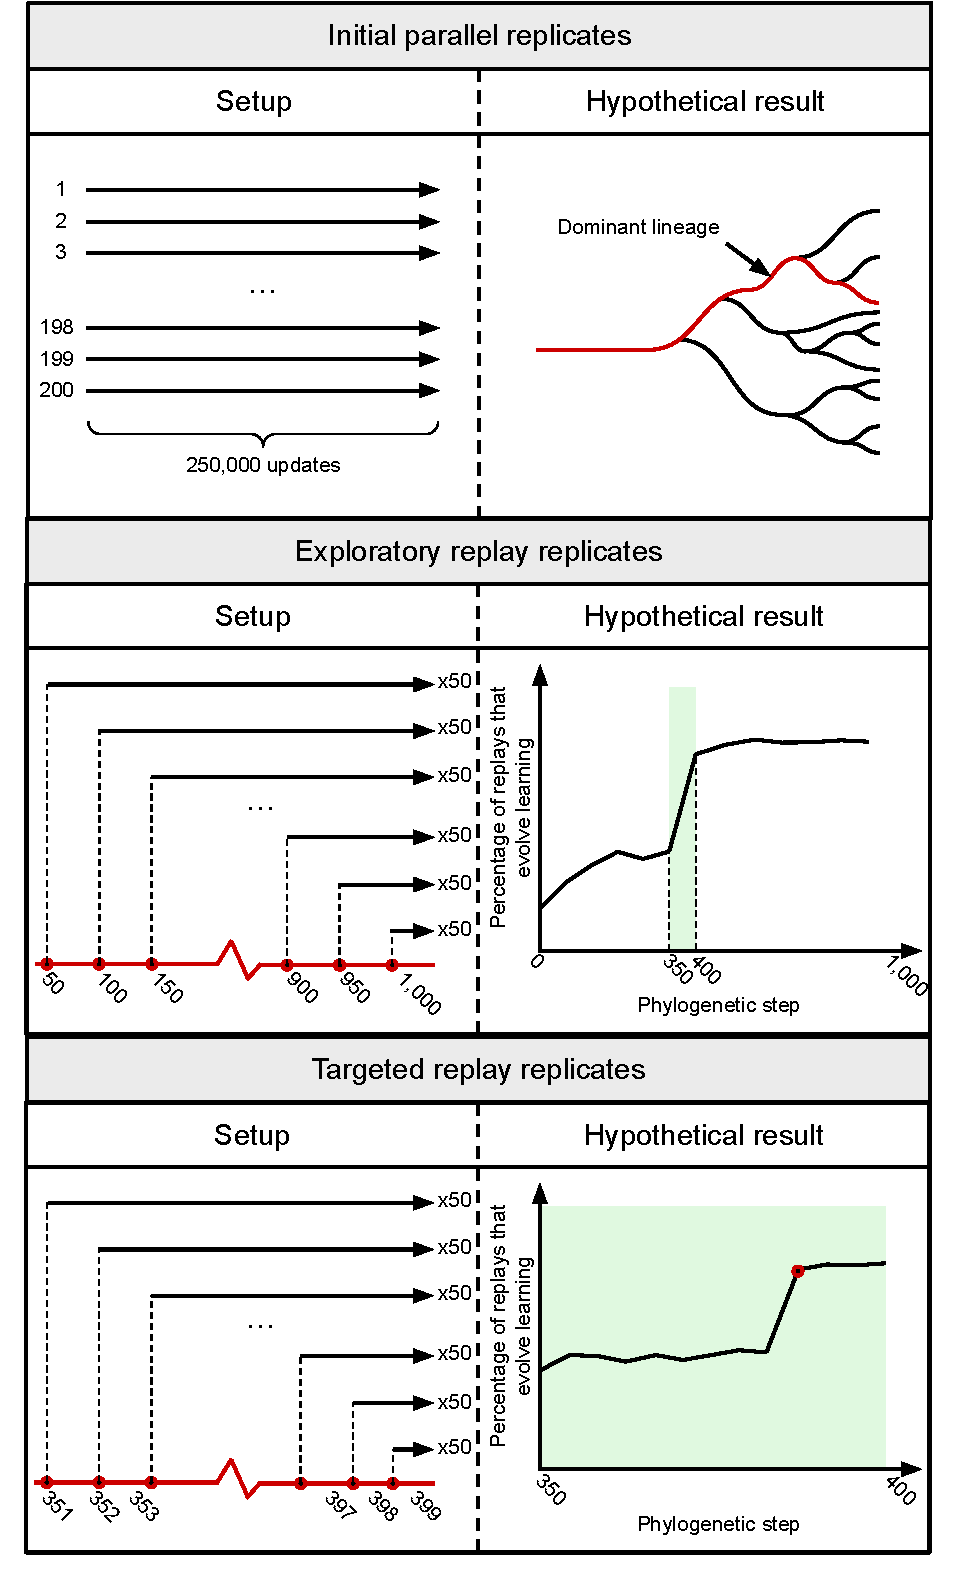
\includegraphics[width=0.65\textwidth]{02_alife_2023_submission/media/conceptual_figure.pdf}
\caption{
    Illustration of the experimental design and hypothetical results.
    The top panes show the 200 initial parallel replicates seeded with the ancestral genotype and evolved for 250,000 updates.
    We extracted the lineage of the most abundant genotype in the evolved population (the dominant lineage), shown in red. 
    %When these replicates finish, we can classify each replicate and extract the dominant lineage (in red) from the phylogeny.
    Next, we conducted exploratory replays (middle panes) by launching replay replicates at regular intervals along focal lineages. 
    These exploratory replays give a coarse-grained view of how potentiation changed over a lineage. 
    We identified the window with the largest potentiation gained, shown as the shaded region.
    Finally, we ran targeted replay replicates for every step in this potentiation window. 
    %Phase 2 takes each dominant lineage from Phase 1 and launches replay experiments every 50 steps along the lineage. 
    %An example potentiation graph is shown, where a substantial increase in potentiation occurs between steps 350 and 400. 
    %We then seed \textit{additional} replay replicates for Phase 3, one for each step in the window identified in Phase 2.
    These fine-grained replay replicates show mutations that resulted in large potentiation increases (shown here with a red dot). 
}
\label{fig-conceptual}
\end{center}
\end{figure}

% Introduce three-phase design and give a brief overview of each part
To identify mutations that substantially increased the likelihood that learning evolved, we split the work into three phases (see Figure \ref{fig-conceptual} for an overview).
%
First, we seeded 200 initial parallel replicates in the associative learning environment with a default ancestor only capable of reproduction. 
Each replicate was given 250,000 updates, where one update is the time it takes for all organisms to execute 30 instructions, on average. 
% These replicates evolved for 250,000 updates, where one update is the
% and evolved them for 250,000 updates.
%For each of the 200 replicates, 
We identified the most abundant genotype in each final population to represent the replicate and classified its behavior. 
%By tracking the phylogeny in each replicate, 
We then extracted the ``dominant lineage'', stretching from the ancestor to the representative genotype. 
%(i.e., the \textit{dominant genotype} of that replicate), classified its behavior, and extracted its lineage from the ancestor. 

To begin analyzing changes in potentiation, we ran exploratory replays replicates on four lineages capable of learning.
%Due to the computational cost of these replay experiments, we performed replays on only four learning replicates.
For each, we seeded independent replicates for every $50^{th}$ step in the lineage, up to step 1,000.
All replay replicates evolved in the same associative learning environment, and replays were given the same number of updates as had %equal to the number of updates that 
occurred after that genotype first appeared (e.g., replays for a genotype that appeared at update 150,000 would be evolved for the remaining 100,000 updates). 
Potentiation was measured as the portion of replay replicates that evolved learning. % divided by the number of replay replicates that finished. 
Because replays were seeded with a single organism, some replay populations went extinct before ever reproducing and thus were not factored in (the minimum number of finished replay replicates from a given lineage step was 38, while three case study lineages had a minimum of 48). 

While the exploratory replays provide an overview of how potentiation changed, we dug deeper by running targeted replays to further explore windows of increasing potentiation.
Specifically, we found the 50- or 100-step ``potentiation window'' that sees the largest increase in potentiation in the exploratory results, and seeded additional replays for every step in that range.
These targeted replays were conducted identically to the exploratory replays, only they did not skip steps.
Though computationally expensive, these replays illuminated the impact every genotypic change had on potentiation. 
Running 50 replay replicates per step still results in considerable noise, but we were able to identify mutations that clearly and substantially increased potentiation using these targeted replays.

We hand-analyzed algorithms in all potentiating mutations, here defined as single lineage steps that result in a potentiation increase of 25 percentage points or more.
%These potentiating mutations and other steps around them in the lineages were hand-analyzed to understand the underlying algorithm encoded in each genotype and how changes to that algorithm may have potentiated the lineage. 
Further, we assessed genotype fitness in context of their lineage to identify if potentiation mutations were beneficial, deleterious, or neutral. 
Finally, %mutation analyses were conducted to 
we characterized the local fitness landscape of each genotype (one- and two-mutations out), measuring the presence and fitness of nearby genotypes that would be capable of learning. 
%All two-step mutations were analyzed for each potentiating step and the step before it, to investigate whether the potentiating step increased the presence of learning in the local landscape, increased the benefit of learning, etc. 

% We then took four lineages that exhibited learning and performed exploratory replays.
% These exploratory replays took the learning lineages and conducted a ``coarse-grained'' sampling of the lineage via analytical replay experiments. 
% We ran replay replicates for every 50 steps along the lineage, out to step 1,000. 
% This provided a window into how the likelihood of evolving learning changed over time.%, and importantly, identified any periods of substantial increases in that likelihood. 
% Finally, in we isolated these period(s) of drastic increases in likelihood and ran additional targeted replay replicates in that window (one for each step along the lineage). 
% This would then show us the impact of individual steps along the lineage, potentially highlighting single steps with massive changes in potentiation. 

% % What did our replay experiments look like?
% %\subsubsection{Analytical replay experiments}
% %After identifying the replicates that evolved learning, we can then begin to analyze their evolutionary history. 
% %We tracked phylogenetic data on all extant organisms and their ancestors, so we can trace a line of descent from the final dominant genotype to the original ancestor. 
% %After identifying the replicates that evolved learning, we then started analytical replay experiments.
% %For each learning replicate, we seeded \textit{additional} evolutionary runs along the dominant genotype's lineage. 
% %Lineages are based on genotypes, so each ``step'' corresponds to a reproduction event where one or more new mutations were introduced in the new offspring. 
% %Starting at step 50, we seeded 50 replay experiments at every $50^{\text{th}}$ step up through step 1,000. 

% %Replay replicates evolved to match the 250,000 updates of the initial replicates.
% %Replays starting from early points in the lineage thus saw more new updates than replays from points farther along the lineage. 
% %As an example, if a replay starts from step 200 and the genotype was first seen at update 100,000, we would run the replicates for step 200 for 150,000 updates. 
% %These evenly-spaced replay replicates were than manually inspected for any large jumps in potentiation. 
% %If evidence of large jumps was detected, we then seeded fine-grained replay replicates for every step between the two multiples of 50.

% % \subsubsection{Initial parallel replicates}

% % % General info, 200 reps for 250k updates starting with a default ancestor
% % We stared by founding 200 parallel replicates (see top panels of Figure \ref{fig-conceptual}). 
% % Each replicate started with one organism: the ancestor organism, which consists of 99 no-operation instructions and 1 \texttt{Repro} instruction. 
% % This organism only reproduces itself, it does not interact with the environment and thus cannot receive any rewards or punishment. 
% % Each replicate was given 250,000 updates, where one update is the time it takes for all organisms to execute 30 instructions, on average. 
% % All replicates ran in the same associative learning environment.

% % % Phylogeny tracking and isolating the final dominant genotype + lineage 
% % % CITE Emily? 
% % We tracked pruned genotypic phylogenies for these initial replicates. 
% % Digital evolution has the advantage of perfectly tracking all reproduction events and storing parent-child relationships. 
% % To reduce the storage overhead, we pruned the phylogenies to only track the extant population and any ancestors of those organisms. 
% % In the end, this gave us the lineage from the ancestral organism to any genotype in the extant population at the end of the 250,000 updates. 
% % As a representative of the final extant population, we extracted the most abundant extant genotype (i.e., the dominant genotype of that replicate) and isolated its lineage.



% \subsubsection{Exploratory replay replicates}

% After the initial parallel replicates concluded, we had a set of replicates that had evolved and maintained associative learning at the end of 250,000 updates. 
% Since we know learning evolved along each of these lineages, we are interested in how the \textit{potentiation} for learning changed along the lineages (i.e., at what points along the lineage was lineage more likely to appear than not, and where did the largest jumps in potentiation occur?).
% To investigate these changes in potentiation, we took a subset of these replicates and conducted a batch of coarse-grained replay experiments to look for large gains in potentiation while conserving computational resources.
% For a given lineage, we seeded 50 replay populations at every $50^{th}$ step along the lineage (see the middle panes of Figure \ref{fig-conceptual}.
% Regardless of the length of the lineage, we stopped at step 1,000, only continuing beyond that point if the potentiation had not approached 100\%.

% To measure potentiation at a point along the lineage, we ran the 50 replay replicates and then calculated the percentage of those replicates that evolved learning (e.g., if 30 replays out of 50 evolved learning, that point would have a potentiation of 60\%). 
% These exploratory replay replicates gave us a summary of how potentiation changed over the course of the lineage. 
% More specifically, we could look for windows containing large potentiation increases. 
% If single mutations conferred large jumps in potentiation, we would expect them to occur in windows of substantial potentiation gain.
% Since all lineages started from the same ancestor, the results from the initial parallel replicates were used for step 0 of every lineage to save computational power.

% \subsubsection{Targeted replay replicates}

% Once the exploratory replays were conducted, we had a summary of how the potentiation changed over the course of the lineage. 
% We used this exploratory replays to identify periods of drastic potentiation gain. 
% The exploratory replays occurred at every 50 steps along the lineage, so we identified the 50-step window that resulted in the greatest increase in potentiation (and for the first two lineages we took a 100-step window as to maximize our chances of finding mutations that confer large jumps in potentiation. 

% Once the target window was identified, we repeated the process of running replay experiments. 
% This time we seeded replays from every step along the lineage inside the target window. 
% While computationally expensive, this illuminates the impact every change in genotype had on potentiation. 
% While 50 replay replicates per lineage step still results in considerable variation, we were able to identify mutations that clearly and substantially increased potentiation using these targeted replays. 

% Once a potentiating step was identified, we analyzed various aspects of the genotype and the evolutionary characteristics surrounding it. 
% These potentiating steps and other steps around them in the lineages were hand-analyzed to understand the underlying algorithm encoded in each genotype and how changes to that algorithm may have potentiated the lineage. 
% Further, the genotypes were assessed in context of the lineage to identify if these potentiation events were beneficial, deleterious, or neutral in terms of fitness. 
% Finally, mutation analyses were conducted to characterize the local fitness landscape and its relationship to learning. 
% All two-step mutations were analyzed for each potentiating step and the step before it, to investigate whether the potentiating step increased the presence of learning in the local landscape, increased the benefit of learning, etc. 

% % How did we conduct our mutational analysis?
% %\subsubsection{Mutational landscape analysis}

% Not sure if we'll have real statistics, but we'll definitely have data to upload
\subsection{Data and software availability}

Both the data and the software used to conduct this work are available in the supplemental material \citep{anonymousalifer_2023_7731472}.
Analyses were conducted in the R statistical computing language \citep{r_core_team_r_v4} using the \textit{dplyr} package to summarize data \citep{wickhamDplyrGrammarData2022}.
Data was visualized using the \textit{ggplot2} package \citep{R-ggplot2}.

\section{Results}

Here we discuss the generation and analysis of the initial replicate runs, followed by the more detailed results from each of the four case study lineages.

\begin{figure}[!h]
\begin{center}
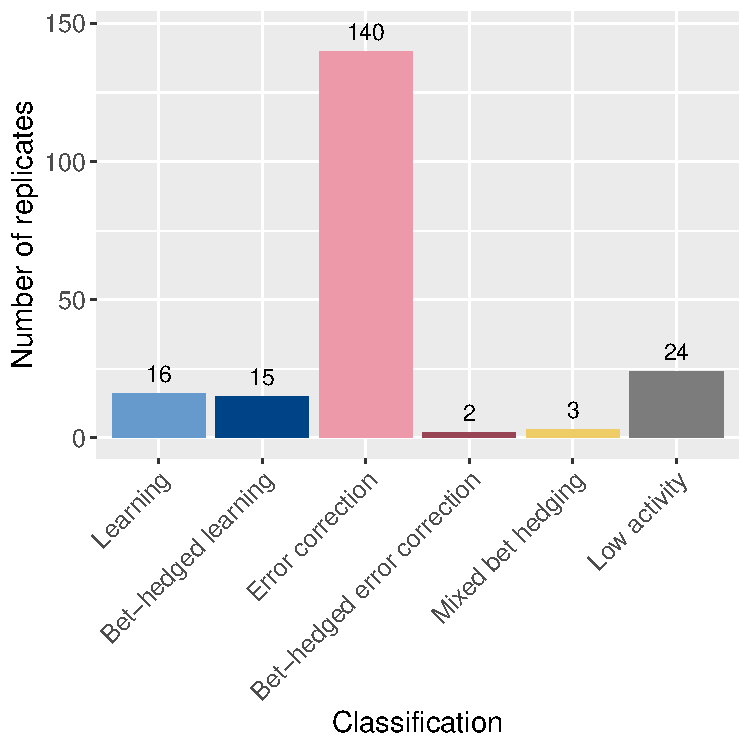
\includegraphics[width=0.45\textwidth]{02_alife_2023_submission/media/final_dom_classification.pdf}
\caption{Behavior classification of the final dominant genotypes from the 200 initial parallel replicates.}
\label{fig-final-dom-classification}
\end{center}
\end{figure}

% \begin{figure}[t]
% \begin{center}
% 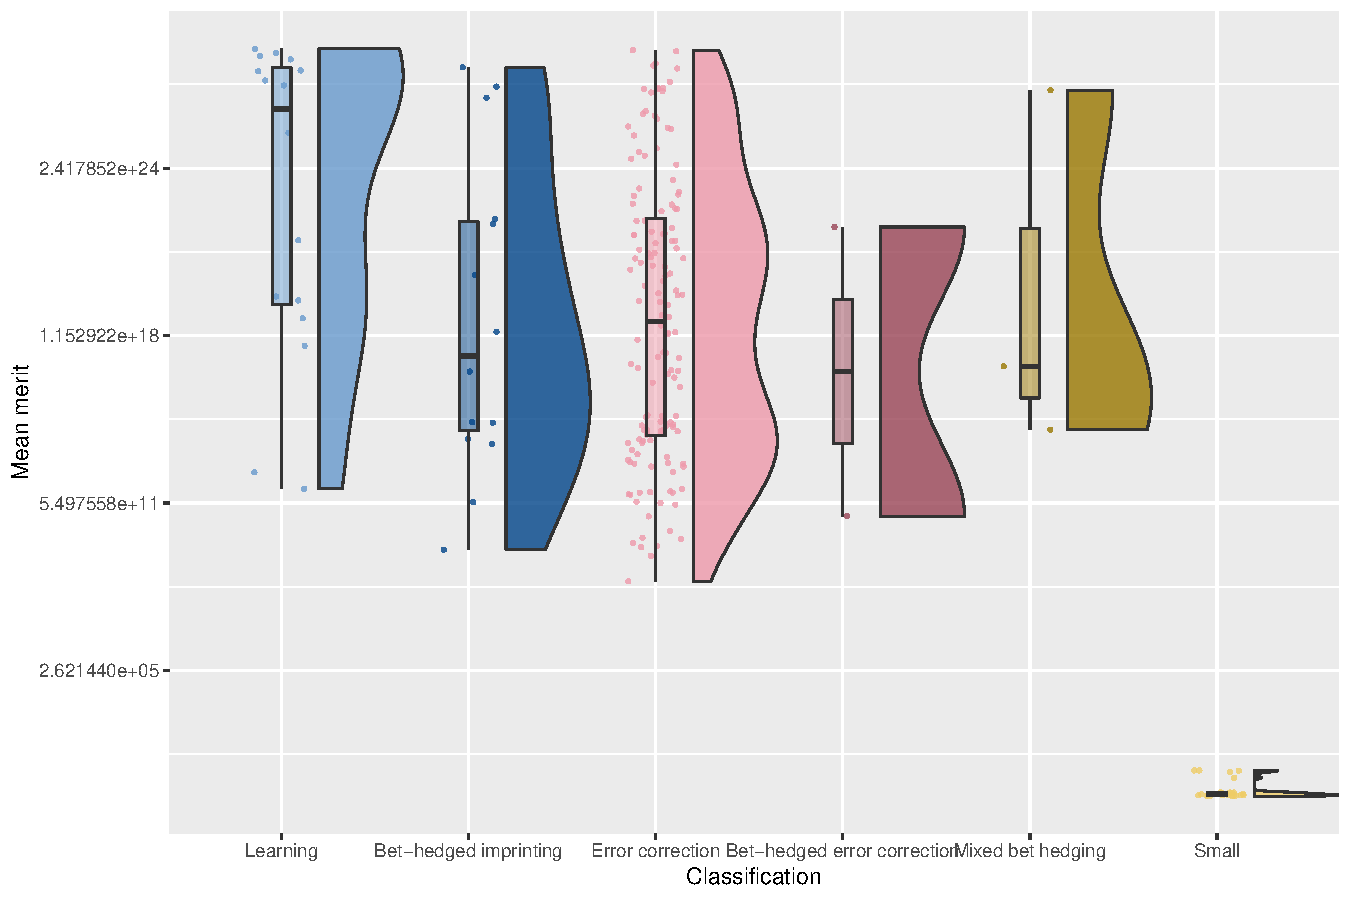
\includegraphics[width=0.45\textwidth]{media/raincloud_rep_merit.pdf}
% \caption{TODO}
% \label{fig-final-dom-rep-merit}
% \end{center}
% \end{figure}

\subsection{Evolution of learning in the initial replicates}
In the first phase of this study, we evolved 200 independent replicates for 250,000 updates (about 3600 generations) in the associative learning domain, each starting with a default ancestor.% capable only of self-replication.
%This setup allowed populations to experience approximately 3600 generations; 
The distribution of evolved behaviors is shown in Figure \ref{fig-final-dom-classification}.
Only 16 of 200 replicates exhibited associative learning.
An additional 15 replicates evolved forms of bet-hedged learning, with two of those replicates gaining and then losing associative learning along their lineage.
The majority of replicates relied on some form of error correction, either as a sole strategy (140), a bet-hedged variant (2), or as a fallback due to limited learning (3). 
%Both bet-hedged error correction replicates have a subset of environments that caused them to fall into cycles of repeatedly choosing the wrong action.%choosing the wrong action, backing up, and then choosing the same wrong action. 
%This prevented them from gaining any additional fitness. 
%Of the three mixed bet-hedging replicates, one exhibited learning in one environment and error correction in the other three
%The other two replicates exhibited the same behavior in all environments: a pseudo-learning strategy that failed on certain sequences of cues and fell back on error correction too often to hit the 90\% accuracy required to be classified as learning.
Finally, 24 replicates failed to navigate enough states to categorize them, leading us to label them as ``low activity''. 

We analyzed all 16 replicates that evolved and maintained learning, identifying the length of their lineages from onset of evolution until learning stabilized, no longer showing further improvement.
Given the substantial computational power required for each time point studied, we performed replay experiments only on the shortest three such lineages (lineages A-C), plus the shortest lineage that exhibited error correction at some point in its evolutionary history (lineage D).
%Of the 16 replicates that evolved and maintained learning, we performed replay experiments on four of them.
%The first three replicates were selected for having the shortest number of steps along a lineage before fitness stopped increasing. 
%The fourth was selected for the same reason, but was selected from among the four replicates that contained error correction in their lineages. 
%These replicates were selected to save computational resources.
%The number of updates experienced by a replay replicate was calculated as the number of updates between the genotype's first appearance in the population and the 250,000 update limit for the initial replicates. 
%Thus longer lineages A) have the potential to require more exploratory replays before saturating to $>90$\% potentiation and B) typically require more updates per replay for early steps in the lineage. 
Selecting these particular replicates to replay has the potential to bias the results, as discussed below.

% \begin{table}[!t]
% \centering
%     {\rowcolors{2}{white}{lightgray!20}
%     \begin{tabular}{ |c|c|c|c|c| }
%         \hline
% %        \makecell{Lineage} & \makecell{Initial \\ seed} & \makecell{Potentiating \\ mutation depth} & \makecell{Potentiation \\ increase} & \makecell{Fitness \\ effect} &  \makecell{Steps before \\ learning} & \makecell{Percentage of \\ updates persisted} \\
%         % \makecell{Lineage} & \makecell{Initial \\ seed} & \makecell{Potentiating \\ mutation depth} & \makecell{Potentiation \\ increase} & \makecell{Fitness \\ effect} &  \makecell{Steps before \\ learning} & \makecell{Potentiating \\ mutation persistence} \\
%         % \hline
%         % A & 86 & 484 & 58pp & Neutral & 53 & 89\% \\ 
%         % B & 4 & 104 & 36pp & Beneficial & 91 & 100\% \\ %1096 (all) \\ 
%         % C & 15 & 279 & 64pp & Deleterious & 26 & 100\% \\ %1978 (all) \\ 
%         % D & 6 & 548 & 50pp & Neutral & 8 & 100\% \\ %589 (all) \\ 
%         \makecell{Lineage} & \makecell{ mutation \\ depth} & \makecell{Potent. \\ increase} & \makecell{Fitness \\ effect} &  \makecell{Steps to \\ learning} \\
%         \hline
%         A & 484 & 58pp & Neutral & 53 \\ 
%         B & 104 & 36pp & $+$ & 91 \\ %1096 (all) \\ 
%         C & 279 & 64pp & $-$ & 26 \\ %1978 (all) \\ 
%         D & 548 & 50pp & Neutral & 8 \\ %589 (all) \\ 

%         \hline
%     \end{tabular}
%     \caption{
%     Summary of targeted replay traits.
%     }
%     \label{tab:replay-summary}
%     }
% \end{table}

\subsection{Case studies of individual lineages}

\begin{figure*}[!th]
    \begin{center}
    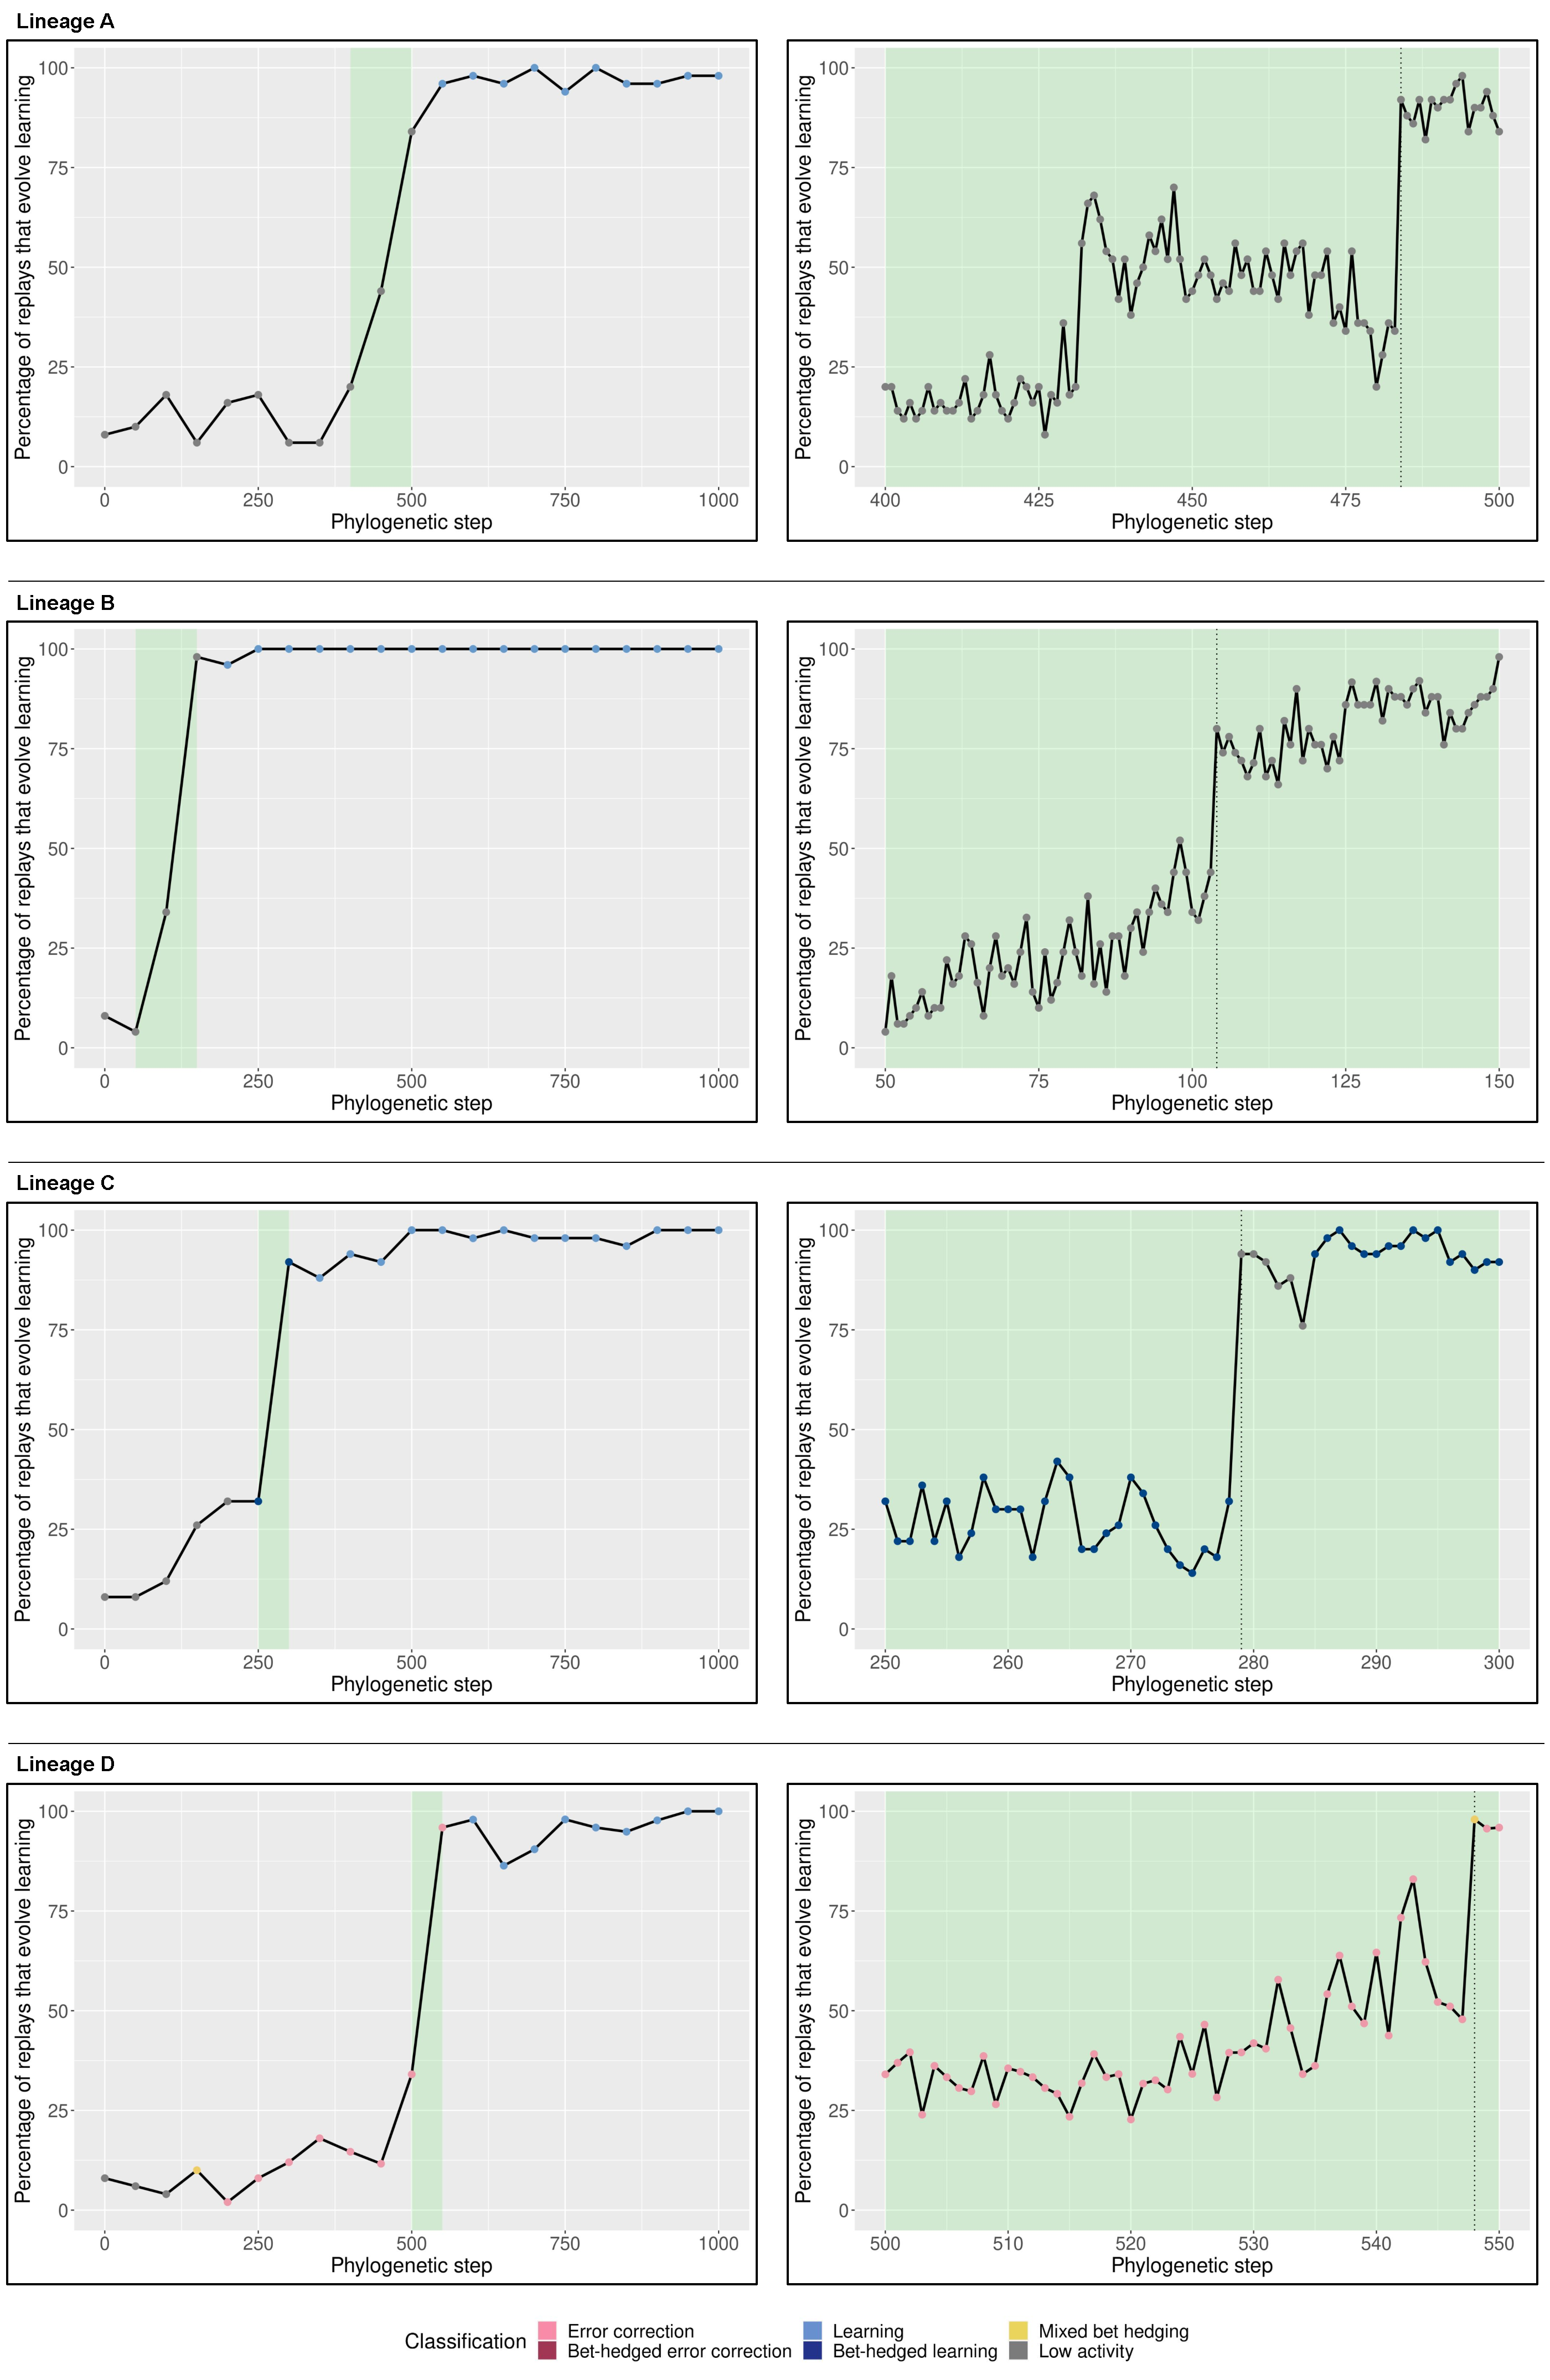
\includegraphics[width=0.72\textwidth]{02_alife_2023_submission/media/combined_replay_plots.pdf}
    \caption{
        Potentiation of associative learning for all case studies, shown as the percentage of replicates that evolve associative learning when evolution is replayed starting at that point.%, as it changes over the lineage for the four case studies. 
        For each case study, the left plot shows the results of the exploratory replays. 
        We identified a window of increased potentiation in each lineage, indicated by the shaded region. 
        Within that window, we conducted targeted replays for every step along the lineage. 
        The results of those targeted replays are shown in the plots on the right.
        The color of the points corresponds to the behavior exhibited at that step of the lineage. 
        A dotted line in the targeted replays indicates the mutation that confers the most potentiation.
    }
    \label{fig-potentiation-all-case-studies}
    \end{center}
\end{figure*}

Below we present the results of the replay experiments performed on the four focal lineages and provide a step-by-step analysis of how key mutations altered both immediate fitness and evolutionary potential (potentiation).
Where possible, we explained how these mutations altered the underlying algorithms.
For each lineage, potentiation across both exploratory and targeted replays can be found in Figure \ref{fig-potentiation-all-case-studies}.
%Additionally, details about the most-potentiating mutation from each lineage can be found in Table \ref{tab:replay-summary}.

\subsubsection{Lineage A}

% \begin{figure}[!h]
%     \begin{center}
%     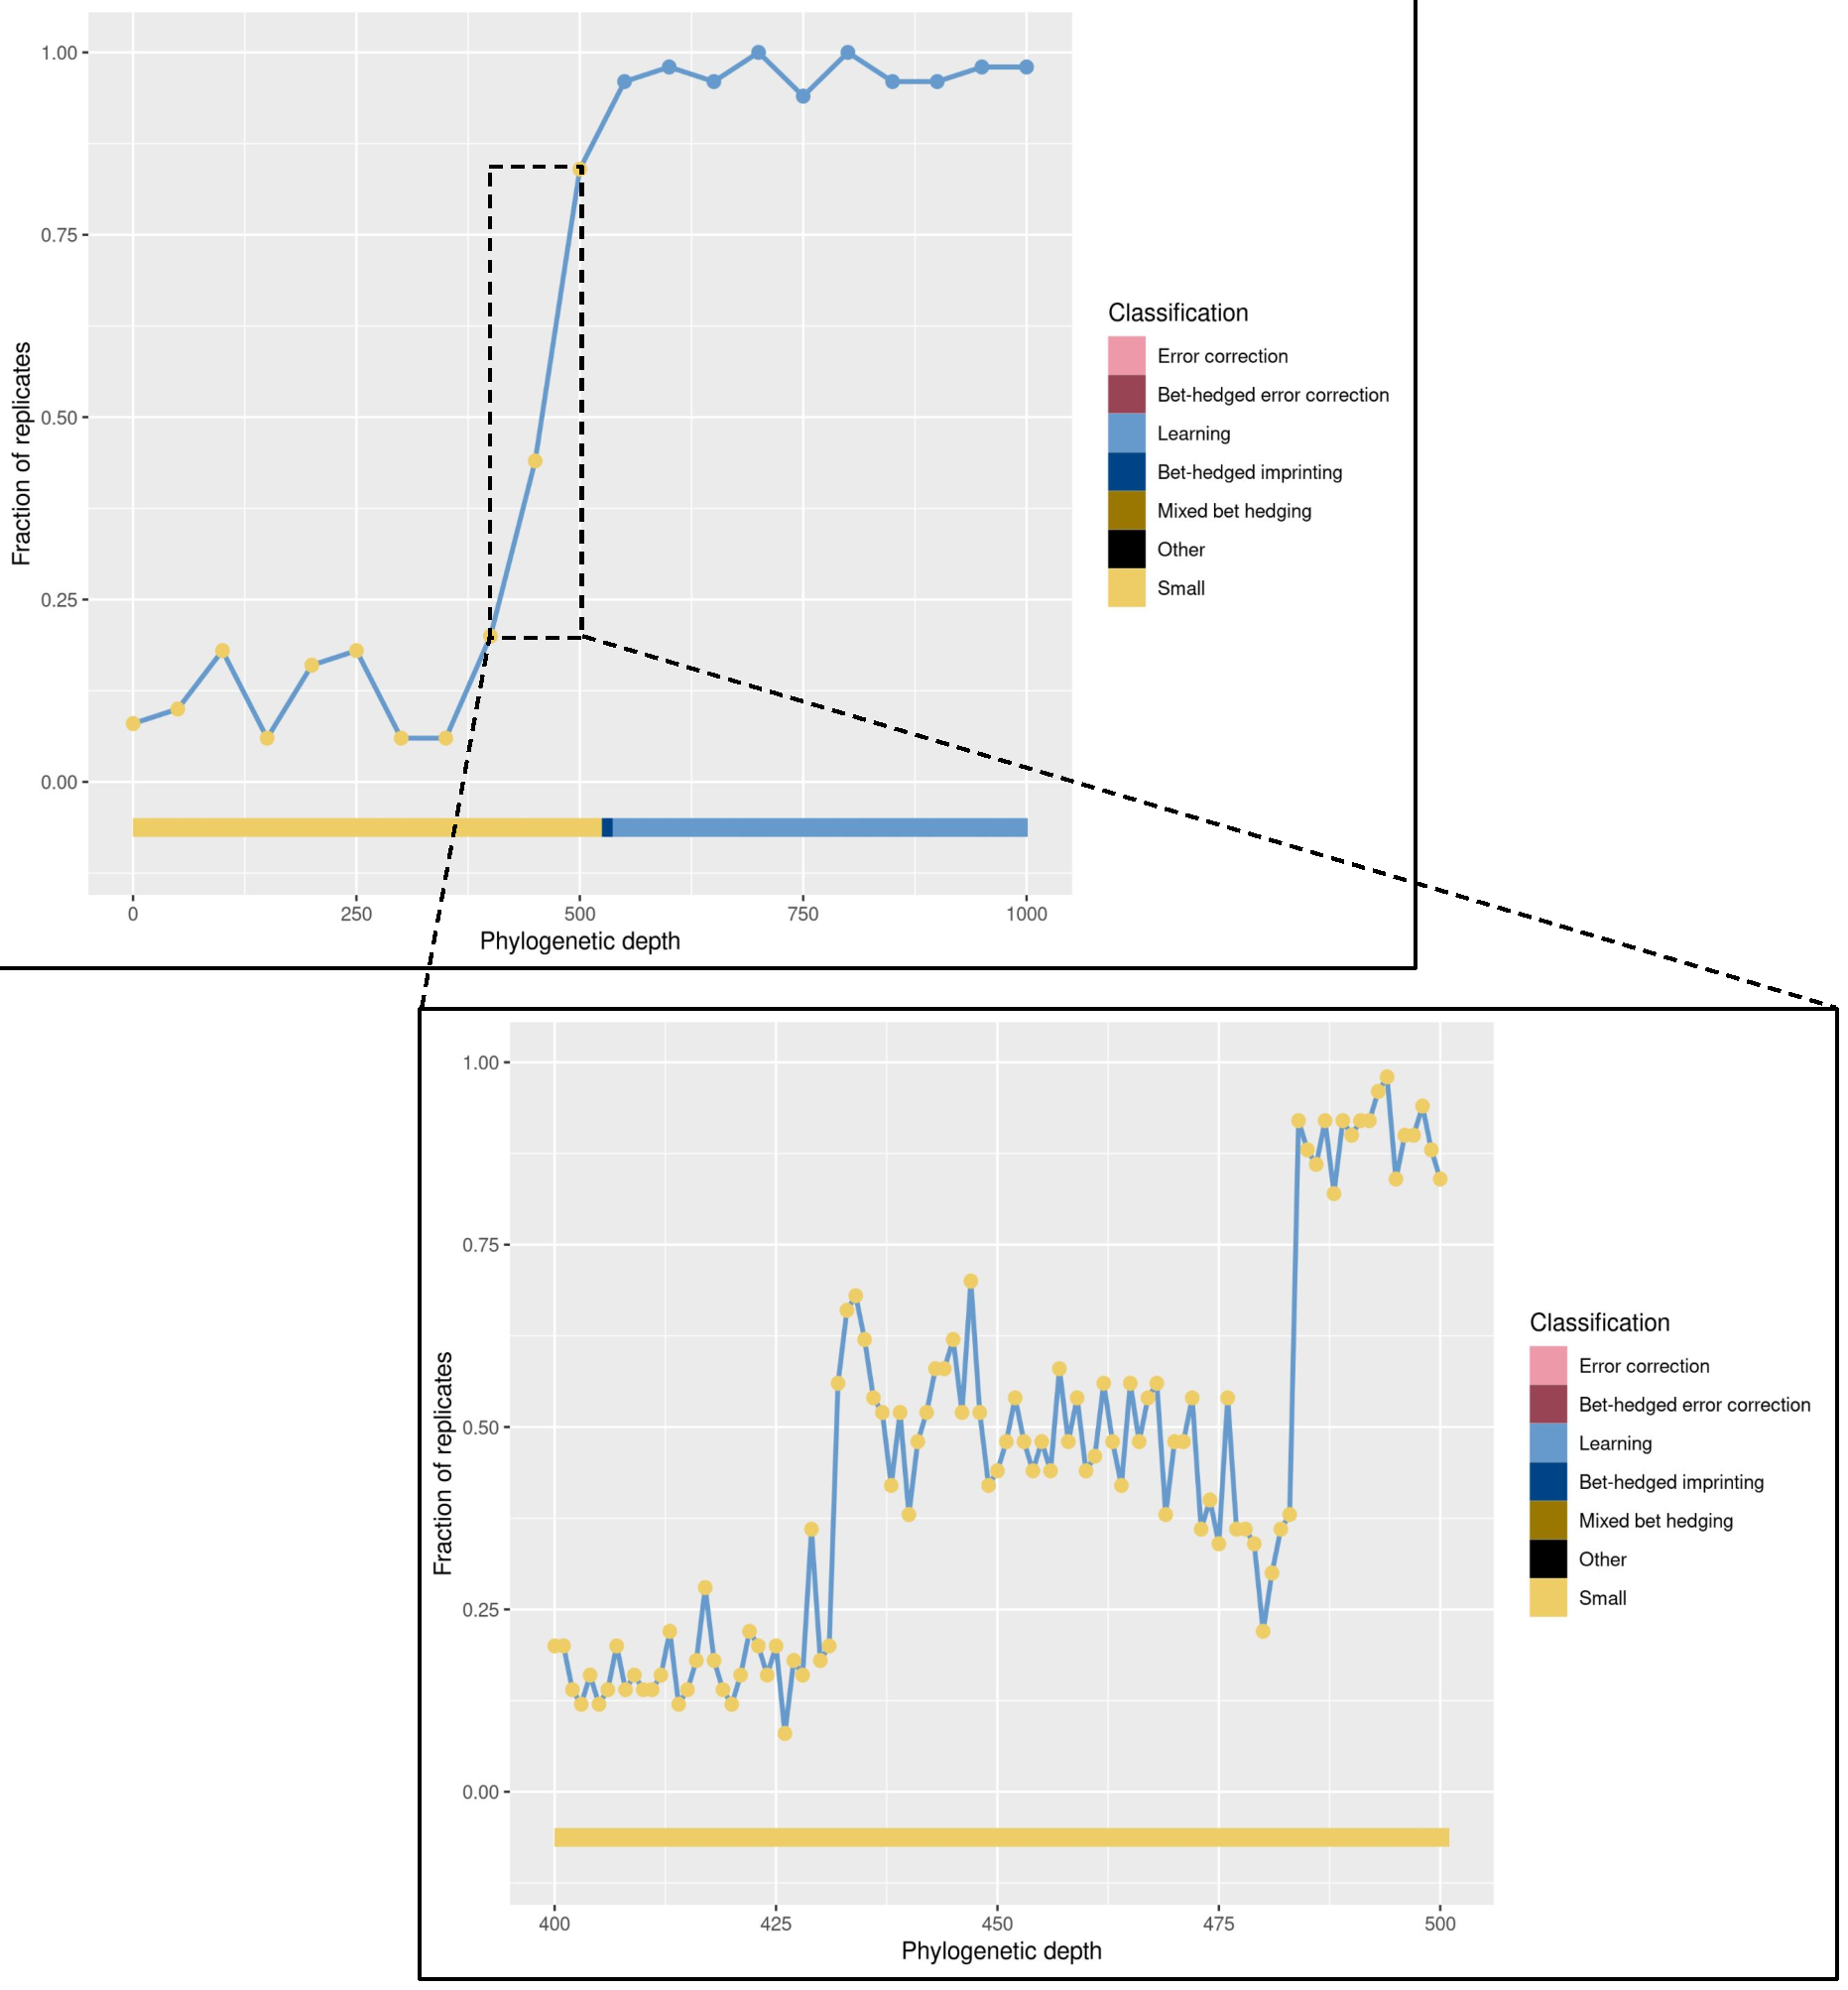
\includegraphics[width=0.45\textwidth]{media/test_pop_out_seed_86.pdf}
%     \caption{
%         \textbf{Case Study A}.
%         Potentiation of associative learning, shown as the fraction of replicates that evolve associative learning when replays are started at that point, as it changes over the lineage for Case Study A. 
%         The top figure plot shows the results of the exploratory replays. 
%         Two windows of increased potentiation were identified, indicated by the dashed rectangle. 
%         Results of the targeted replays are shown in the bottom, pop-out plot.
%         Both lines and points show potentiation at various steps along the lineage. 
%         The color of the points corresponds to the behavior exhibited at that step of the lineage.
%         The rectangle at the bottom of the plot also shows the behavior at the lineage, but with more detail than the evenly spaced points of the exploratory replay.
%     }
%     \label{fig-potentiation-case-study-a}
%     \end{center}
% \end{figure}

Our first case study is one of the shortest lineages and it contains a quick jump to learning (at step 537) from low activity, with only a brief time spent in bet-hedged learning. 
%The exploratory and targeted replays for Case Study A are both shown in Figure \ref{fig-potentiation-case-study-a}.
Exploratory replays for this lineage revealed a stark jump in potentiation between 400 and 500 steps from the ancestor, which we call the potentiation window.
From step 400 to step 450, potentiation increased from 20\% of replicates to 44\%, and increased again to 84\% of replicates by step 500. 
Before this window, potentiation fluctuated around the original 8\% found starting from the default ancestor.
%Before this jump, the potentiation fluctuates between 6\% of replicates and 20\% of replicates evolving learning. 
After the selected window, potentiation increased once more and then fluctuated between 94\% and 100\%. 

With this in mind, we seeded 50 replays for each genotype in the potentiation window. 
%Since we run 50 replicates at each step, there is considerable noise in the data. 
%Regardless, two mutations confer drastic increases in potentiation: steps 432 and 484. 
Even with the noise due to a small sample size, %that comes from having only 50 replays at each step,
we identified two mutations that conferred sizable increases in potentiation: steps 432 and 484.
The mutation at step 432 brought potentiation above 50\% for the first observed time in the lineage. 
Surprisingly, potentiation then decreased (on average) back to a local minimum of 20\% of replicates at step 480. 
Finally, the mutation at step 484 substantially increased potentiation to 92\%, where it stayed for all subsequent replays. 
%Looking at performance averaged over 100 trials, both mutations are neutral in fitness.

Even though the largest jump in potentiation occurred at step 484, learning did not appear in the lineage until step 537. 
That said, only steps 516 and 525 caused any change in behavior; all other interim mutations occurred in unexecuted regions of the genome. 
The potentiating mutation at step 484 made a key instruction in the main loop of the genome redundant.
It had no immediate effect on fitness, but later (in intermediate step 516) allowed the redundant instruction to be replaced by
%, mutating the redundant instruction into 
a right turn that granted a small fitness increase as organisms could now navigate until they reached the second left turn. 
Step 525 further improved navigation, but used a comparison that made an unfounded assumption on whether the left or right random cue is larger. 
When the assumption was correct organisms were capable of learning the cues, however the assumption is only correct 50\% of the time, so this genotype is categorized as bet-hedged learning. 
Finally, step 537 swapped that comparison with one that makes no assumptions about cue values, enabling the genotype to learn in all environments.%and now the genotype can always learn. 

Looking at the local mutational neighborhood, the potentiating mutation at step 484 increased the number of two-step mutations that conferred learning from 2 to 9 (of approximately 56 million). 
Additionally, the fitness of the learning mutations in the local neighborhood increased by three or four orders of magnitude.
%Specifically, the mutation at step 484 adds a \texttt{Decrement} instruction at the very first position in the genome. 
%This makes another \texttt{Decrement} instruction in the midst of the main section of the genome obsolete, as it was only called once and now is never called because of the new mutation. 
%With that locus now free to mutate, step 516 sees a mutation at that exact locus, swapping it to a \texttt{Right} movement instruction.
%This allows organisms to move right for the first time, which they do successfully a few times before being stumped by a \textit{left} immediately followed by a \textit{right}.
%Finally, the mutation to learning at step 537 adds more flow control before the new \texttt{Right} instruction, alleviating the issue and allowing organisms to cleanly handle any sequence of states. 
%These three mutations saw a shift from less than 7 correct states, on average, at step 484, to less than 10 at step 516, to over 115 at step 537, resulting in a drastic fitness increase.
%While was purely neutral in fitness when it occurred, the mutation at step 484 shifted the genetic material to allow changes to the vital machinery and paving the way for learning. 

What about the earlier potentiation that was gained and then lost?
The mutation that substantially increased potentiation at step 432  introduced a comparison that had no immediate fitness effect. 
This comparison remained unimportant until step 525 when it became integral in introducing bet-hedged learning.%interacted with that new comparison to improve the algorithm. 
%Looking at two-step mutations, neither step 432 nor the step before had any learning in their local landscapes. 
Neither step 432 nor its predecessor had access to learning within a two-step mutational range.
Thus, it is likely that the potentiation comes from that comparison given that we observed it being utilized for learning later on.

%The earlier potentiation at step 432 swapped a \texttt{Push} instruction for an \texttt{IfLess} instruction. 
%At the time, this did nothing. 
%In fact, this instruction only comes into play at step 537, where it becomes part of the logic of ``if B does not equal C AND C is greater than or equal to 3, then take a right turn''. 
%Thus, while it took a while to get there, the mutation was directly useful in the learning algorithm. 

%[MOVE TO DISCUSSION???]
Why then, did potentiation decrease between steps 432 and 484?
At step 432 (and indeed before it), the algorithm had a section where if register B was non-zero, then B stored the cue associated with a left turn. 
While this information was likely to make the evolution of learning easier, it was unused at that time. 
As such, the mutations between steps 432 and 484 dismantled that machinery, requiring a replacement to be built before learning could evolve.

%increasing the number of mutations needed for learning to evolve. 
%Indeed, this machinery was rebuilt before learning evolved, but in a different way. 

\subsubsection{Lineage B}

% \begin{figure}[!h]
% \begin{center}
% 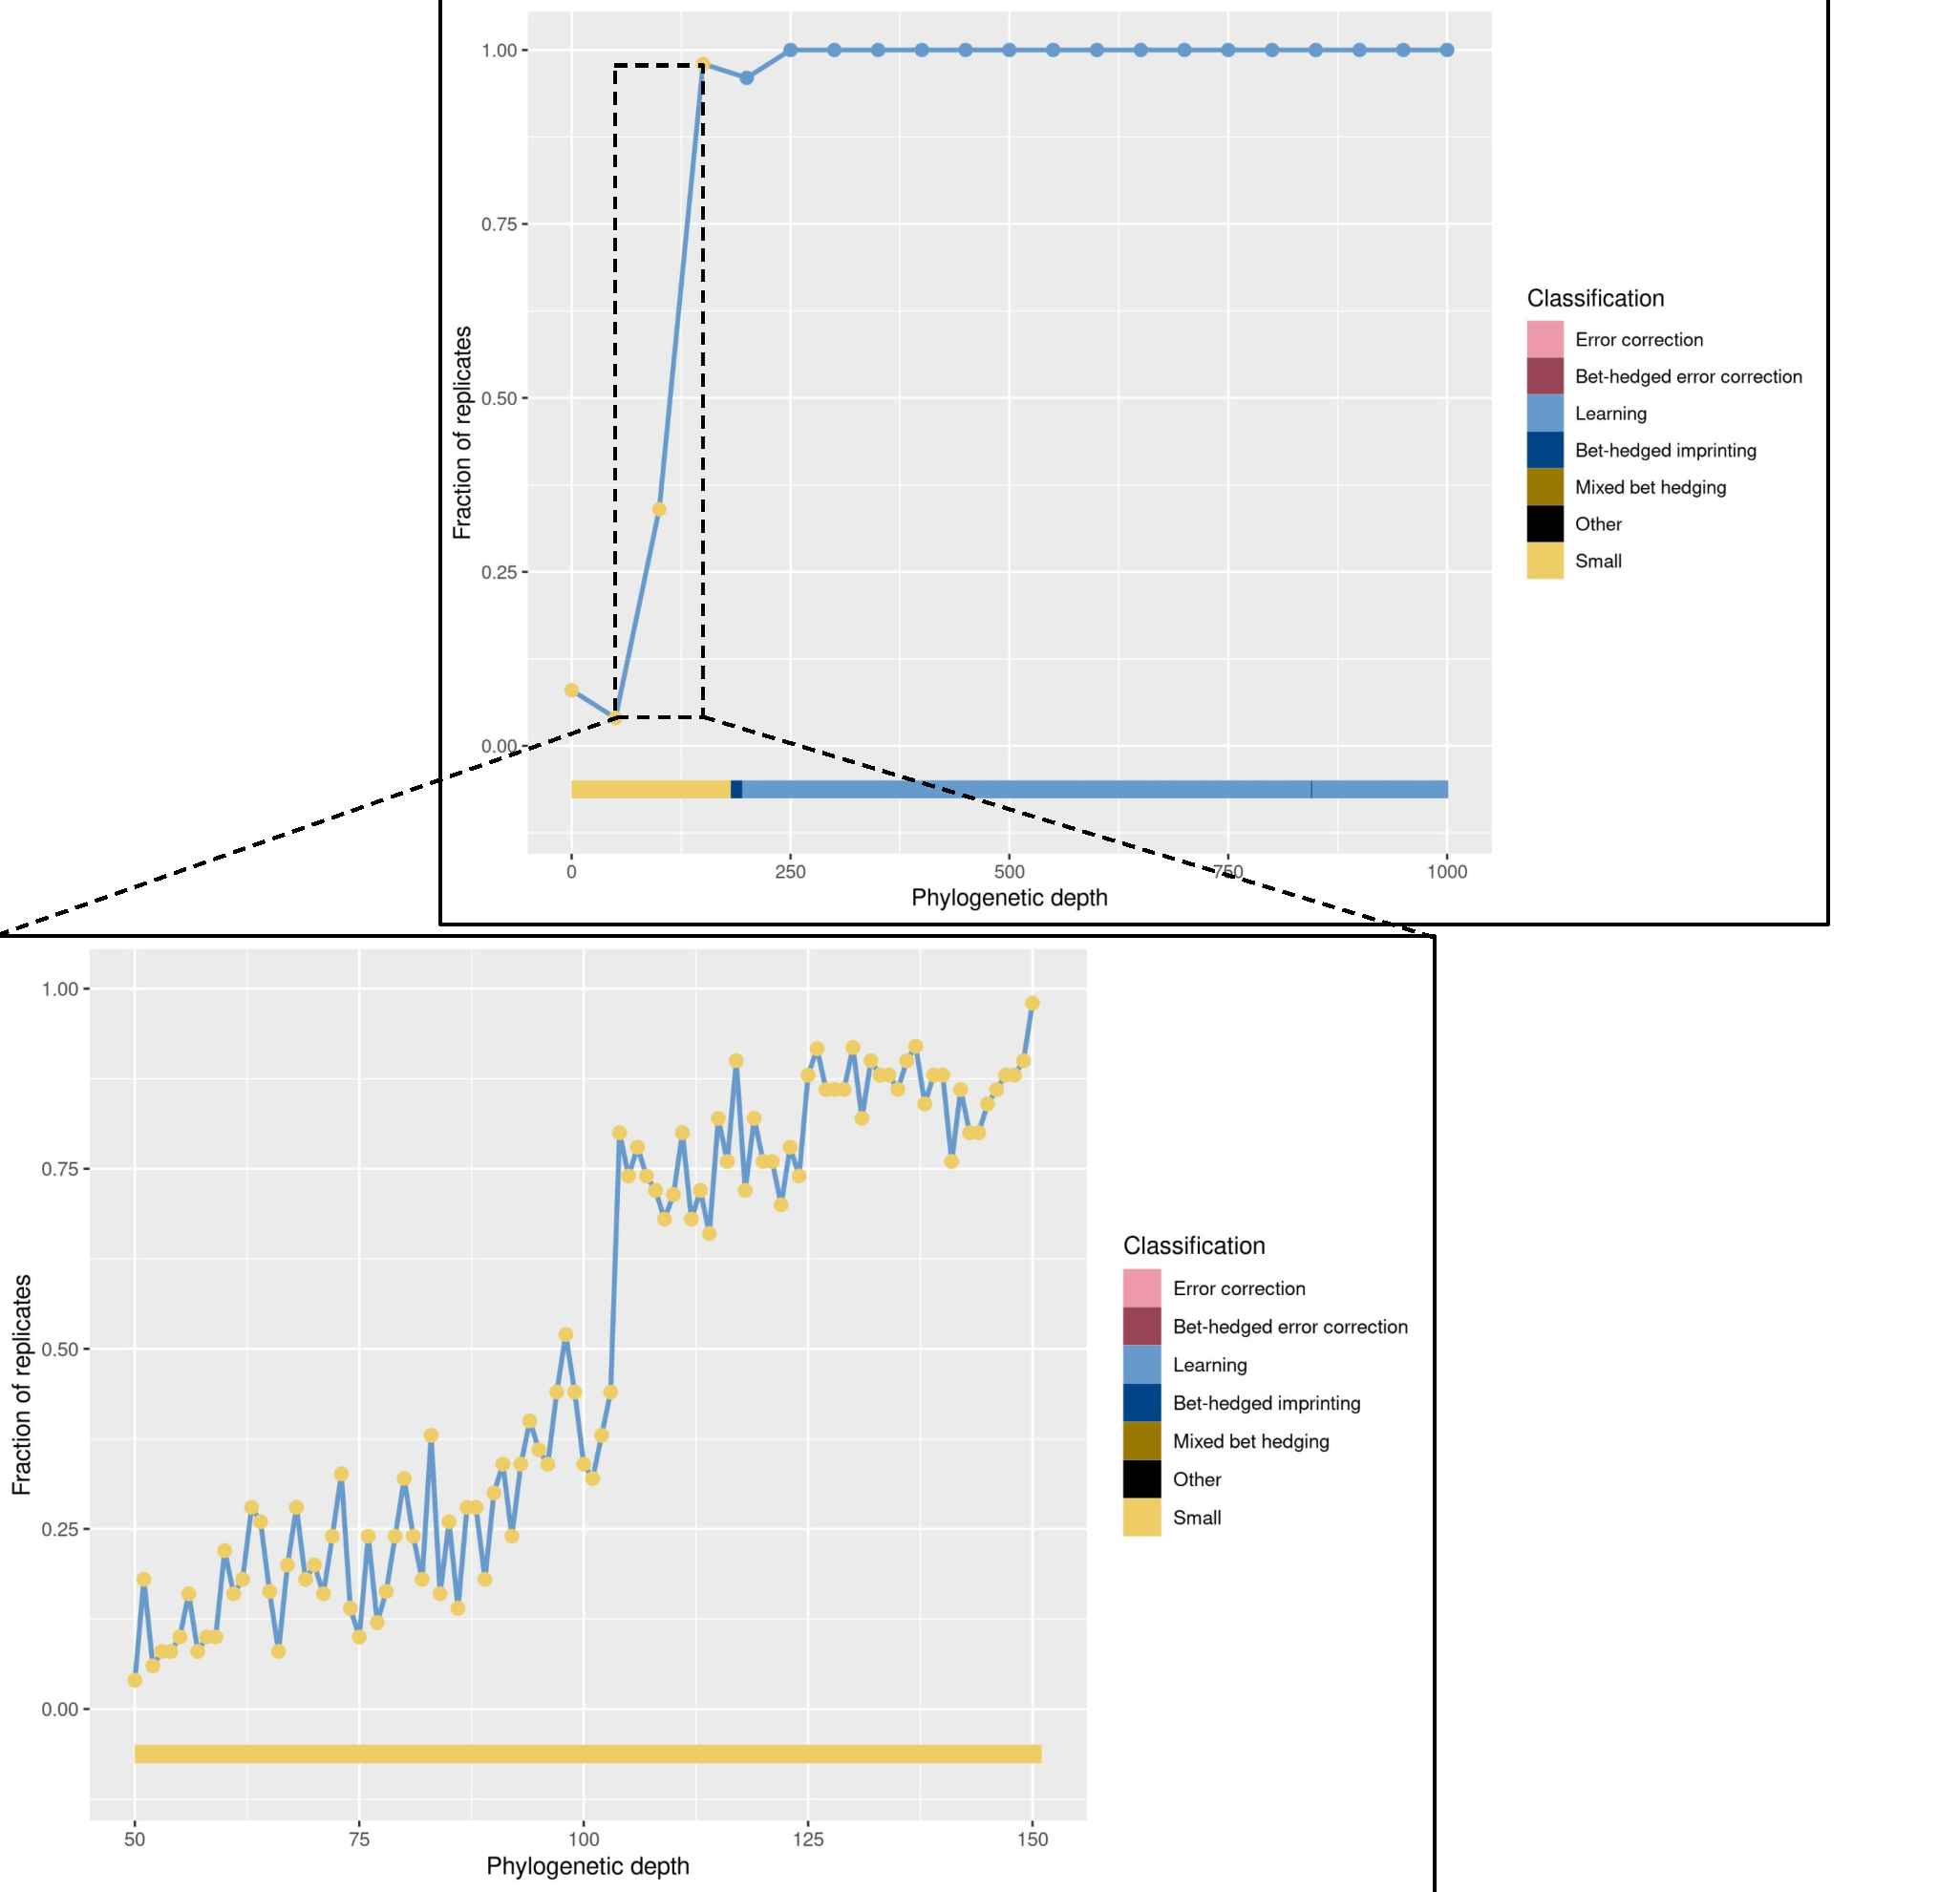
\includegraphics[width=0.45\textwidth]{media/test_pop_out_seed_4.pdf}
% \caption{
% \textbf{Case Study B}.
% Potentiation of associative learning as it changes over the lineage for Case Study B. 
% The top figure plot shows the results of the exploratory replays. 
% Two windows of increased potentiation were identified, indicated by the dashed rectangle. 
% Results of the targeted replays are shown in the bottom, pop-out plot.
% Both lines and points show potentiation at various steps along the lineage. 
% The color of the points corresponds to the behavior exhibited at that step of the lineage.
% The rectangle at the bottom of the plot also shows the behavior at the lineage, but with more detail than the evenly spaced points of the exploratory replay.}
% \label{fig-potentiation-case-study-b}
% \end{center}
% \end{figure}

Similar to Lineage A, this lineage transitioned from low activity to learning through a brief period of bet-hedged learning. 
Exploratory replays on this lineage reveal that learning was potentiated almost immediately; by step 150 potentiation had climbed above 95\%, where it stayed for the rest of the lineage. 
%From this exploration we identified 
As such, the potentiation window included steps 50 through 150.%, and therefore targeted that windows for additional replays. 

Unlike Lineage A, the targeted replays reveal a general trend of increasing potentiation, with step 104 as a notable outlier. 
%However, one mutation stands out as an outlier: step 104. 
Mutations from steps 50 through 103 slowly increased potentiation from 4\% to 44\%, but the mutation at step 104 jumped it to 80\%. 
From there, another slow increase continued to raise potentiation to a peak of 98\% at step 150.

Learning did not appear until step 195, over 90 steps beyond the largest potentiating mutation. 
Given that 34 interacting mutations altered the encoded algorithm, the mechanistic pathway to achieve learning is more complicated than can be broken down in this work.
%breaking down the exact details of the changes to reach learning is beyond the scope of this work. 
However, the potentiating mutation at step 104 modified the execution flow of the genome, which appears to have been later used essential for the later evolution of learning.% in the long term. 

While two mutations occurred at step 104, only one caused a functional change: an instruction to swap data between registers was mutated to a left turn. 
Prior to this mutation, the genome encoded a left turn later on, after which the execution became trapped in an endless loop. 
The potentiating mutation was immediately beneficial; it allowed organisms to take the left turn earlier, which, in turn, allowed them to avoid the loop. 
%As such, this mutation was immediately beneficial when it occurred. 
In avoiding the infinite loop, a large portion of the genome was now skipped and remained so when learning evolved 91 steps later. 
Looking at the local fitness landscape, learning was neither present in the potentiating step's landscape nor in the step before.
We hypothesize that the potentiation came from the change in structure of the genome, that skipping the execution of those instructions avoided a pitfall and freed up execution time that may have been useful in evolving learning.

%While two mutations occurred at step 104, only one provides a functional change. 
%That mutation is a point mutation swapping a \texttt{Swap} instruction for a \texttt{Left} movement instruction. 
%Another \texttt{Left} instruction already existed a little further along the genome, but removing the \texttt{Swap} instruction allowed execution to jump back to the main portion of the genome, while still executing the needed left turn before doing so. 
%This increased fitness immediately, as it prevented the organism from getting stuck in an infinite loop at toward the end of the genome, instead correctly handling a few more states. 
%Secondly, this caused a large portion of the genome to not be executed, most of which is still skipped when learning evolved at step 195. 
%The mutation at step 104 did prove important, as it persisted throughout evolution, being present in the final genome at step 1544.


\subsubsection{Lineage C}

Lineage C has the biggest single-mutation potentiation increase (64 percentage points), and that mutation was deleterious when it occurred at step 279 along the lineage.  Learning later appeared at step 305. 

The potentiating step mutated a no-operation instruction into a conditional flow control instruction. 
%On the existing genetic background, this mutation was terrible for fitness.
At step 278 the genotype was capable of bet-hedged learning, but the mutation at 279 knocked out all instances of learning, reclassifying the lineage as ``low activity.'' %down below the classification threshold. 
The next step restored some fitness, and then step 285 interacted with the mutation at 279 to not only restore fitness, but to dramatically improve it. 
Ultimately, the potentiating mutation allowed the algorithm to more precisely discriminate between the left and right cues. 
Prior to the mutation, it used a less-than comparison, which only functioned correctly in tests where the ``turn left'' cue was less than the ``turn right'' cue. %left the algorithm at the mercy of the random cue values. 
The potentiating mutation switched it to an equality comparison, which alleviated the assumption that one cue will be larger than the other.

Interestingly, the potentiating mutation both lowered the number of learning mutations available in the local fitness landscape and decreased the average fitness of the learning mutants that do exist. 


% When learning appears at step 305, it comes in the form of a \texttt{Decrement} instruction being swapped for a \texttt{Subtract}.
% These genotypes cannot fix their mistakes, they rely on never making errors. 
% Steps 285 through 304 cannot handle two \textit{left} states in a row, but step 305 can. 
% By using subtraction instead of decrement, the algorithm is able to always zero out the register, which combines with the flow control and ensures the algorithm can handle multiple left turns in a row.



% \begin{figure}[!h]
% \begin{center}
% 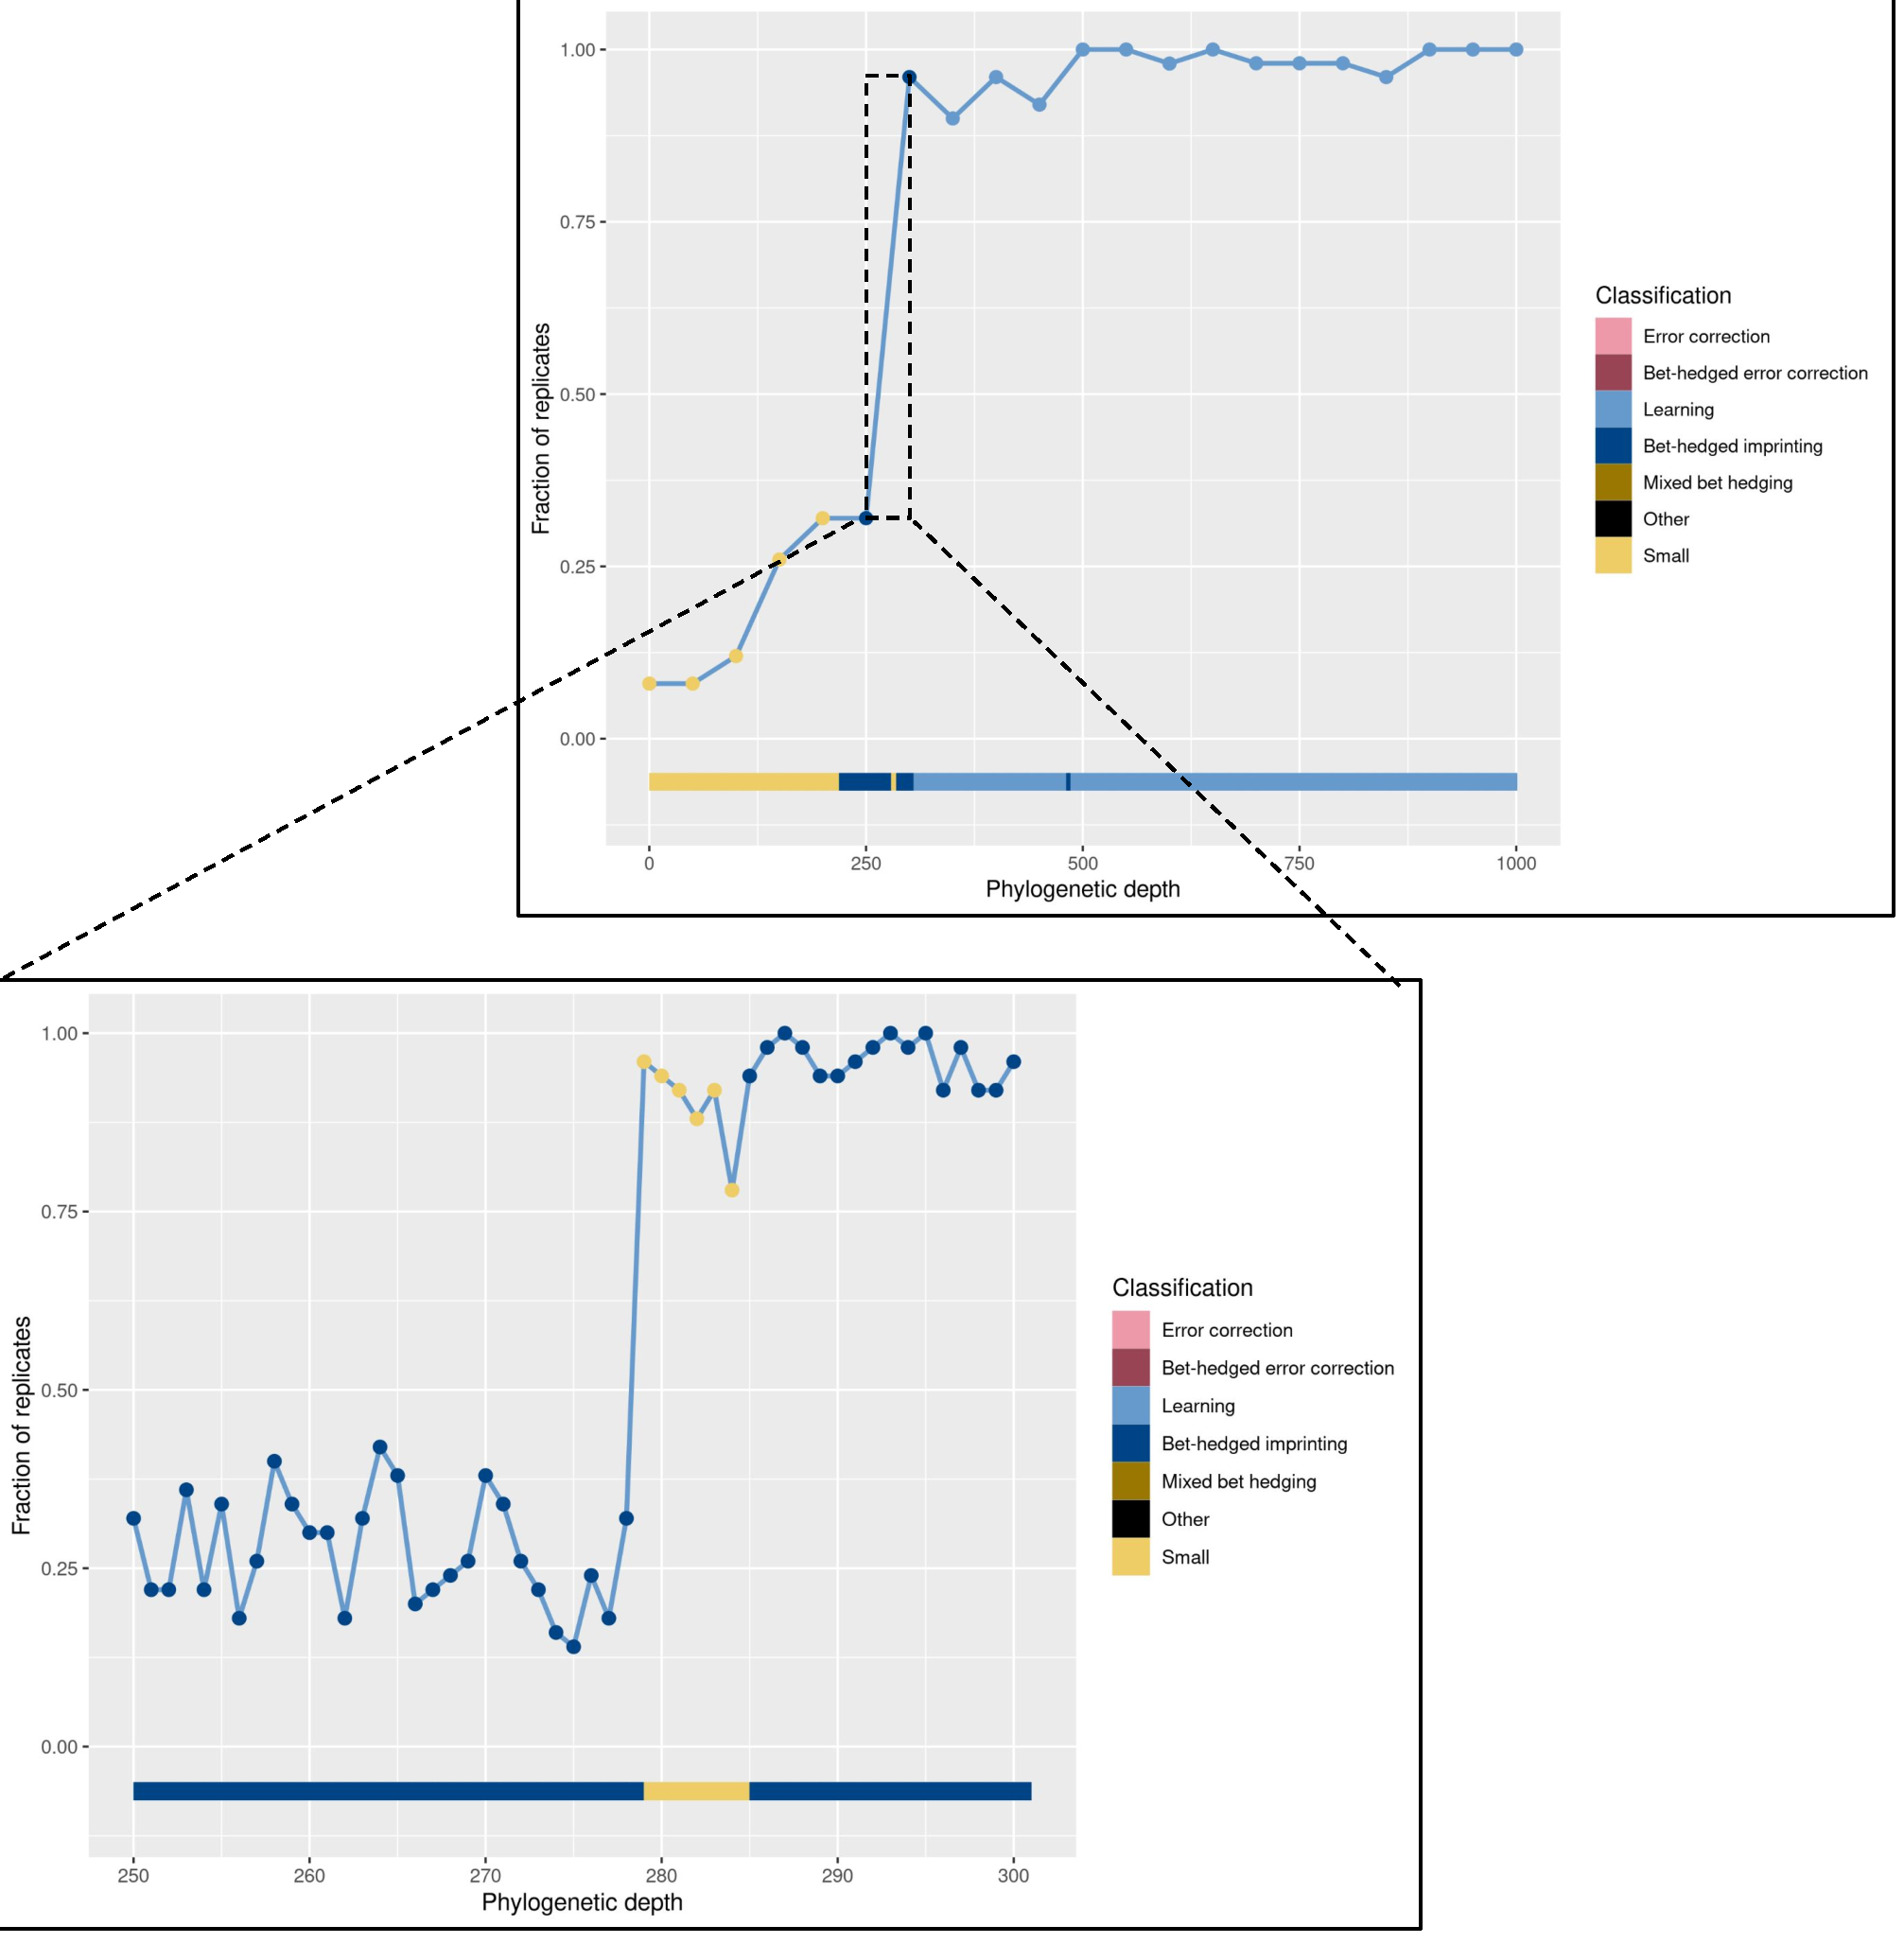
\includegraphics[width=0.45\textwidth]{media/test_pop_out_seed_15.pdf}
% \caption{
% \textbf{Case Study C}.
% Potentiation of associative learning as it changes over the lineage for Case Study C. 
% The top figure plot shows the results of the exploratory replays. 
% Two windows of increased potentiation were identified, indicated by the dashed rectangle. 
% Results of the targeted replays are shown in the bottom, pop-out plot.
% Both lines and points show potentiation at various steps along the lineage. 
% The color of the points corresponds to the behavior exhibited at that step of the lineage.
% The rectangle at the bottom of the plot also shows the behavior at the lineage, but with more detail than the evenly spaced points of the exploratory replay.}
% \label{fig-potentiation-case-study-d}
% \end{center}
% \end{figure}




\subsubsection{Lineage D}

% \begin{figure}[!h]
% \begin{center}
% 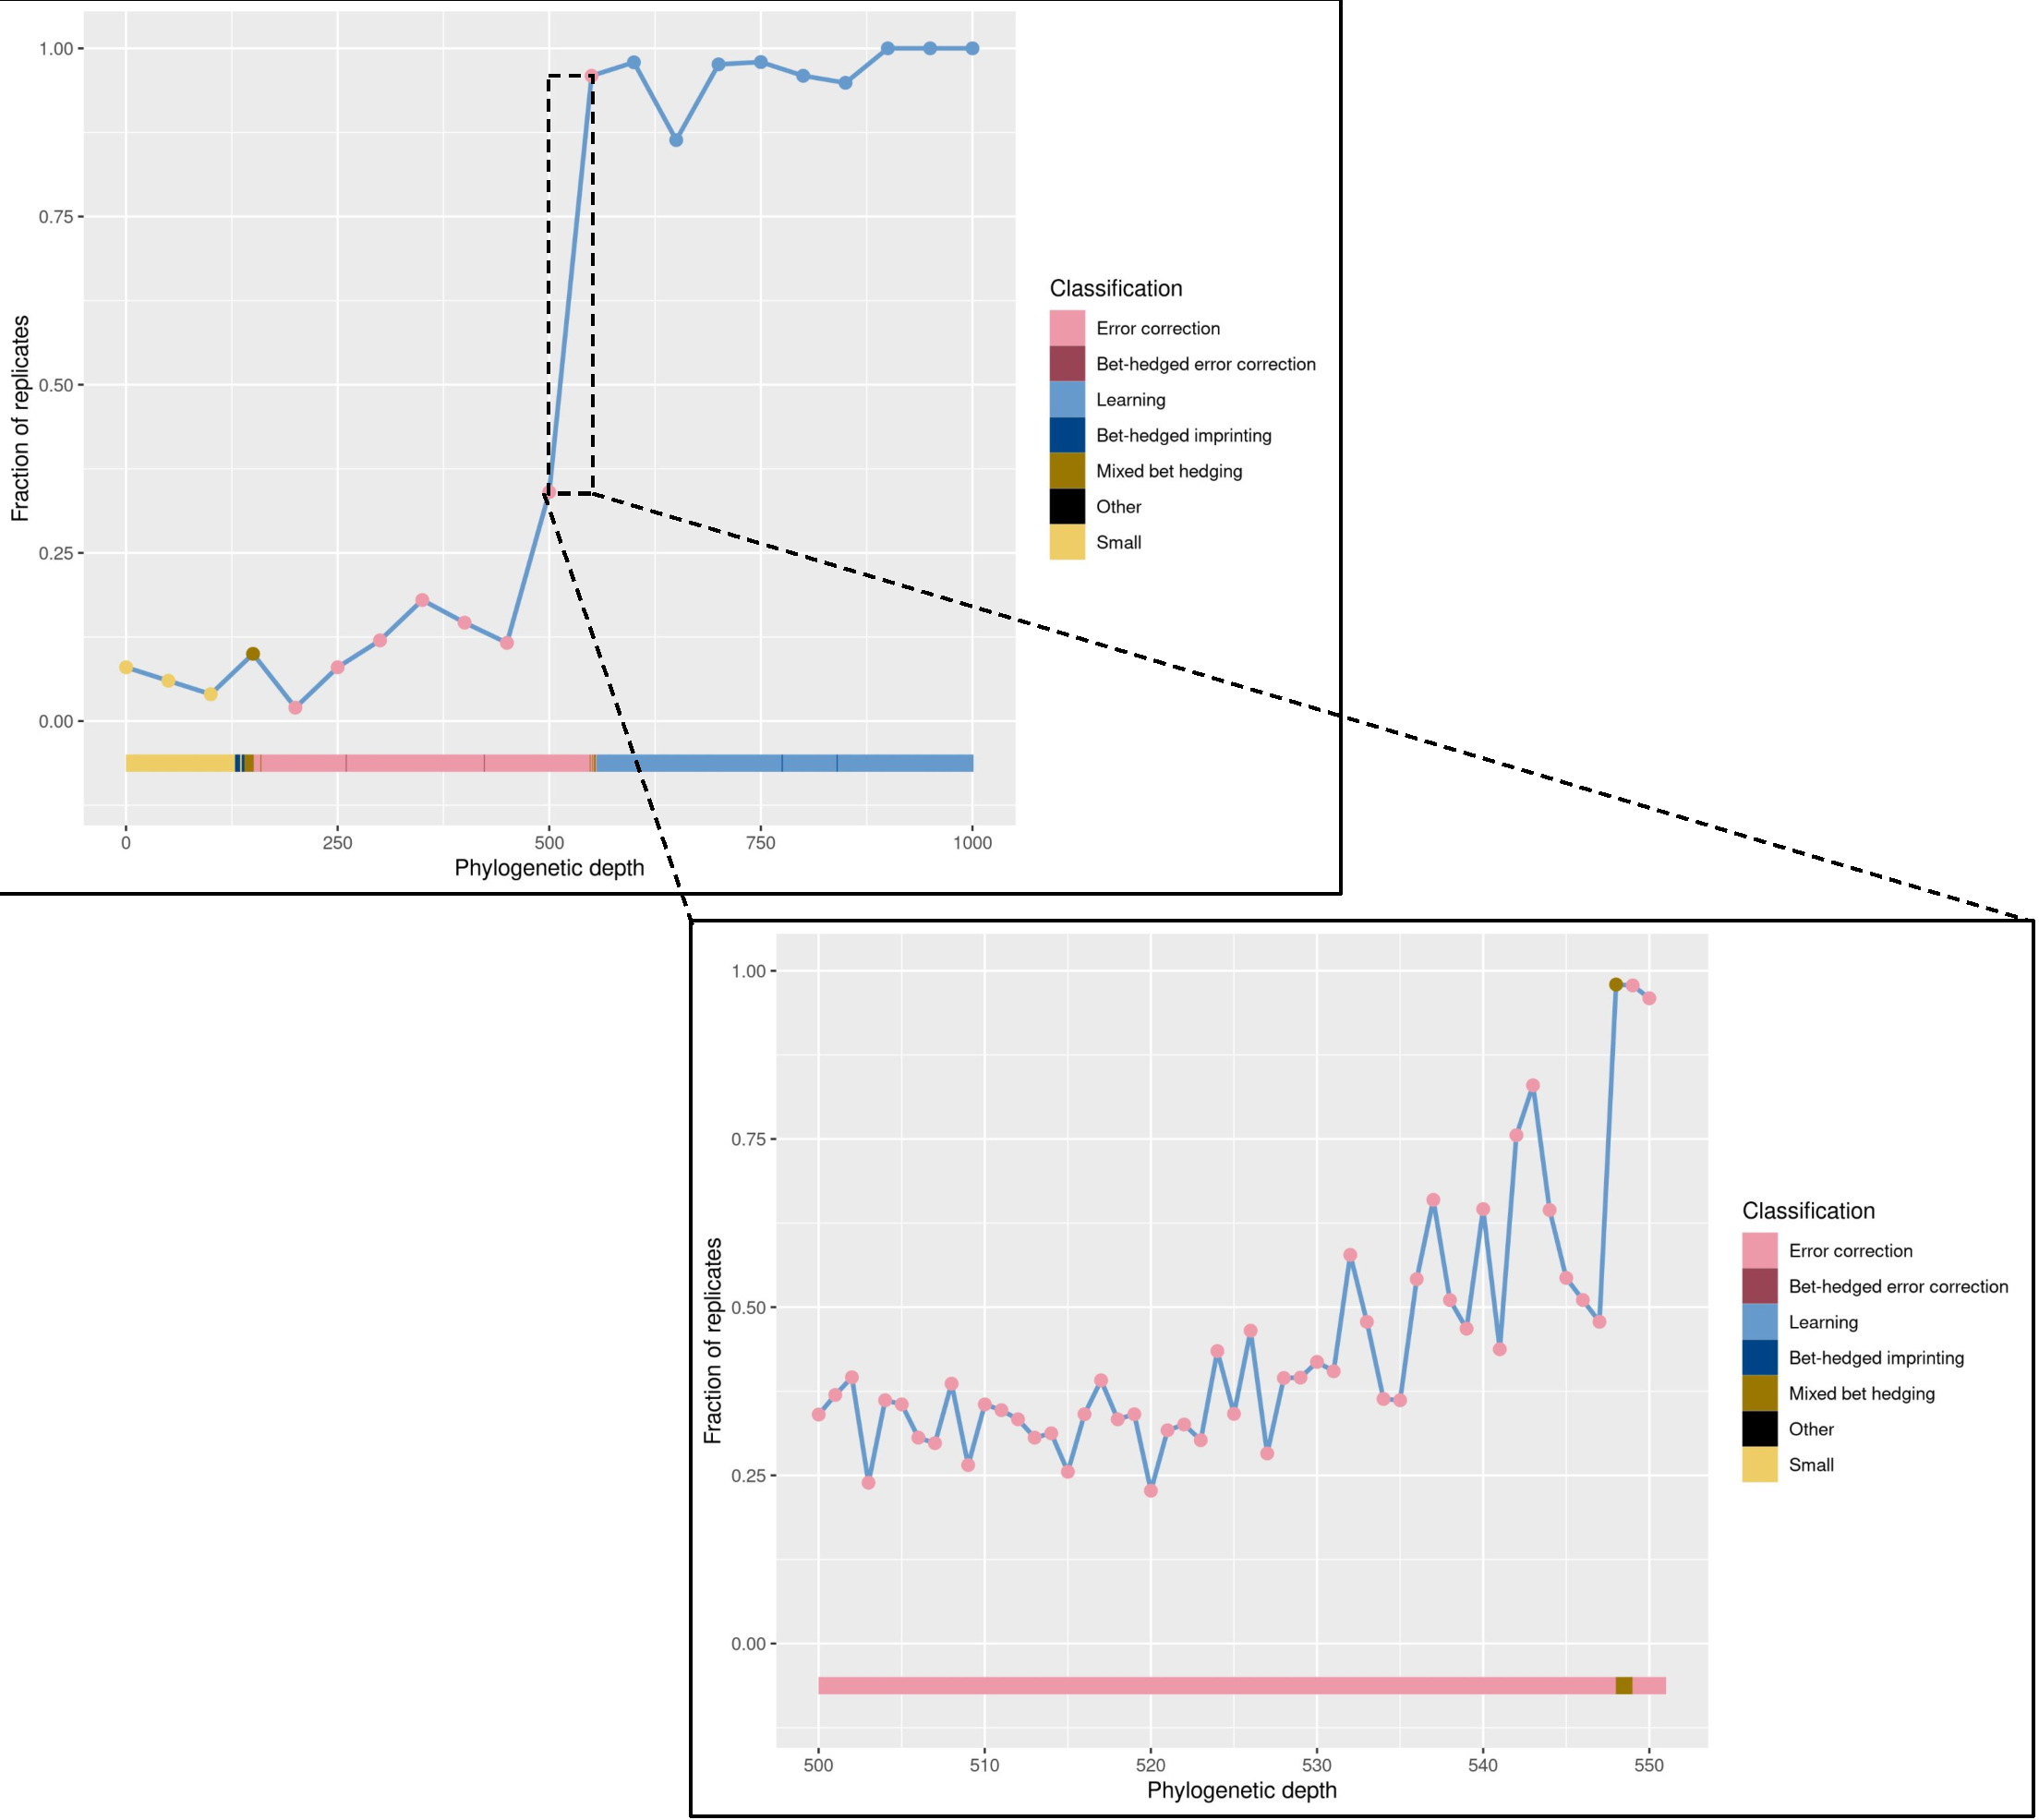
\includegraphics[width=0.45\textwidth]{media/test_pop_out_seed_6.pdf}
% \caption{
% \textbf{Case Study D}.
% Potentiation of associative learning as it changes over the lineage for Case Study D. 
% The top figure plot shows the results of the exploratory replays. 
% Two windows of increased potentiation were identified, indicated by the dashed rectangle. 
% Results of the targeted replays are shown in the bottom, pop-out plot.
% Both lines and points show potentiation at various steps along the lineage. 
% The color of the points corresponds to the behavior exhibited at that step of the lineage.
% The rectangle at the bottom of the plot also shows the behavior at the lineage, but with more detail than the evenly spaced points of the exploratory replay.}
% \label{fig-potentiation-case-study-d}
% \end{center}
% \end{figure}

Of the four replicates we analyzed, Lineage D is the only one that evolved error correction before learning.
Like the earlier lineages, the exploratory replays show that almost all potentiation comes from a single window. 
%Here, however, we only study the back half of the window, where 
In this case, potentiation grew from 34\% of replicates to 96\% between steps 500 and 550.
%Zooming in via targeted replays, potentiation in this window tells an interesting story. 
%It is hard to be certain given the noise of using 50 replay populations, but it appears that potentiation generally increases in the second half of the window. 
Targeted replays are especially noisy for this lineage, but generally show an increase in potentiation, especially in the latter half of the window.
%Of particular note are the last \~10 steps in this window. 
The largest jump in potentiation occurred at step 548, near the end of the window.
%Looking backward, however, other 
Prior mutations also showed notably increased potentiation, but in each case later mutations appeared to lower potentiation again. % before later mutations lowered it again. 
Specifically, steps 542 and 543 appear to have higher potentiation than the points around them, with potentiation dipping back below 50\% again before the largest jump at 548.

Out of all four lineages, D has the fewest steps between the largest potentiating step (548) and the first appearance of learning (556).
At the time, the potentiating mutations at 548 caused no discernible change in fitness even though they increased potentiation by 50 percentage points. 
Two mutations occurred at step 548: a point mutation swapped a flow control instruction for a math instruction and an insertion mutation added a comparative conditional instruction into the main execution loop. 
At step 548 the genotype encoded a naive error correction algorithm: after setup, organisms could always handle \textit{turn right} states, but always failed \textit{turn left} states, recovered, and then continued. 
%This changed when learning evolved 
At step 556, the algorithm started sensing the environment, albeit \textit{too} often. 
A mutation swapped a sensing instruction with a math instruction, and this combined with the prior comparison instruction from step 548 to allow the organism to move left when needed. 
The organism still blundered when it encountered a state sequence of \textit{left}, \textit{forward}, \textit{left}, but it quickly recovered. 
Since it can associate the cues with greater than 90\% accuracy, we classify it as learning. 
The local fitness landscape supports the idea that the comparison instruction was useful to the evolution of learning, as the potentiating mutation increased the number of learning genotypes in the two-step mutational neighborhood from under 800 to over 100,000.

% What's going on at 542/543?
Looking back at the apparent false start at steps 542 and 543, it is not clear what algorithmic changes these mutations conferred.
%, the potentiation mutations at steps 542 and 543 also altered 
These steps did, however, alter the set of learning behaviors that fell within the local mutational neighborhood. 
At step 541, there were only 324 two-step mutations that conferred learning, and only three of those resulted in a substantial fitness increase (a merit $> 10^{15}$). %; the merit of the best-performing mutant is ~$1.6e21$.
After steps 542 and 543, that number rose such that over 900 two-step mutations could confer learning, with over 500 resulting in a substantial fitness increase (including over 200 that reached a merit $> 10^{25}$.
We may be unsure of the exact effects of these mutations on the mechanics of the algorithm, but the changes in the local fitness landscape are profound. %to include learning algorithms with much higher fitness.


\section{Discussion and Conclusion}

%\subsection{Some mutations are potentiating.}
\subsection{Potentiation can rise suddenly}

% What evidence do we have?
We have documented several cases where wherein single mutations dramatically increased the probability of associative learning later evolving.%arising in the longer term.
Of the four lineages analyzed, each had a single step in the lineage that resulted in a substantial increase in potentiation (ranging from 36 to 64 percentage points). 
Indeed, two of the lineages had an additional potentiating mutation that resulted in an increase of over 30 percentage points.
Limiting ourselves to exploratory replays, each lineage has a 50-step window that resulted in a potentiation increase of at least 40 percentage points.

% What does this mean?
% What does the literature say about potentiation?
While four lineages are insufficient to make any strong claims, these results demonstrate that it is \textit{possible} for single mutations to drastically increase potentiation, and provide compelling evidence that they may, in fact, be common. 
In Lineages B and D, however, we do also observe regions with smaller, incremental increases in potentiation.
Further studies are clearly necessary to more fully understand the general patterns and processes by which potentiation rises across different representations and environments.
%We do not claim that all potentiation comes from one or a few mutations, simply that future work cannot disregard the possibility that a large chunk of potentiation comes from a single mutation.


%\subsection{Some mutations are anti-potentiating.}
\subsection{Potentiation can decrease along a successful lineage}

In two of the lineages we analyzed (A and D), we see evidence of potentiation decreasing over spans of the lineage. 
%We also see mutations that decrease the probability of associative learning appearing.  
%Specifically, Lineages A and D both see jumps in potentiation that are then lost over the next section of the lineage. 
With only 50 replay populations per lineage step, our results are noisy and it is difficult to isolate what is occurring during these periods of potentiation decline.
While we were unable to identify any ``anti-potentiating'' mutations with effects as large as the positive potentiation mutations, it is possible for a single step in a lineage to greatly decrease potentiation. 

%Future work should investigate this concept of decreasing potentiation. 
Since we limited our analyses to runs where associative learning arose in the original replicate, we did not expect a preponderance of anti-potentiating mutations, but were intrigued to see evidence of them, even if at low effect.  
%However, these mutations could exist. 
These same analytic replay experiments could be applied to lineages that failed to evolve the target behavior, to see if potentiation on that behavior experiences sudden drops. 
Similarly, our replays targeted windows with substantial increases in potentiation; other windows would be more likely to include decreases. 
Finally, failed replays from starting points with otherwise high potentiation must have failed for a reason; they too could be used as a likely source (albeit more artificial) of anti-potentiating mutations.
%Windows that see a large decrease in potentiation are more likely to contain anti-potentiating mutations, while windows of little or no potentiation change early in a lineage have the potential of an increase and subsequent decrease of potentiation within that window.
%One hypothesis is that potentiation-decreasing mutations are beneficial when they occur, and that the instant gain in fitness comes at the detriment of long-term success of evolving the complex behavior. 

%That said, in run BLAH we do see a period of steady decline in the probability of associate learning arising, though no individual mutations has a dramatic negative effect.  
%If we were to focus our replay experiments more broadly, we expect that many of the runs that never produce associative learning may exhibit more signs of anti-potentiating mutations and we plan to investigate this further in the future.

%\subsection{Potentiating mutations vary substantially from one evolutionary lineage to another}
%[Step through the different runs and talk about how different the patterns are.  Can even look at some of the runs that got associative learning, but we didn't zoom in on yet.]



\subsection{Potentiating mutations can appear innocuous when they first occur}

%[Step through these mutations and discuss how they have different immediate effects and nothing immediately identifies them as potentiating.  End with the question of "so, how are these mutations any different from other mutations?"  To have any chance of identifying potentiating mutations ahead of time, we must first further understand the underlying mechanisms that make them potentiating.]
We analyzed the mutational step in each of the four lineages that conferred the greatest increase in potentiation.
Of those four mutational events, two were neutral, one was deleterious, and one was beneficial. 
Even among these few replicates, there is no obvious pattern in the properties of potentiating mutations. 
Of the two neutral mutations, one made an instruction redundant while the other added a conditional instruction that had no effect when it was initially introduced. 
The deleterious and beneficial mutations both caused the execution flow to loop back earlier than it did before.
Additionally, the number of mutations between the potentiating mutation and the appearance of learning varied wildly between lineages, ranging from 8 steps up to 91.
The potentiating mutations in these four lineages are unique, and at the current time there is no pattern emerging among them.
So, how are these mutations any different from other mutations?
Untangling this mystery could be critical for predicting evolutionary outcomes or accelerating adaptive evolution.


% \subsection{What makes a mutation potentiating?}
\subsection{We can identify \textit{how} a mutation is potentiating}

There are many mechanisms by which a mutation could facilitate the evolution of associative learning.
For example, the mutation could provide a building block that is helpful to perform the task.  
But for a mutation to be potentiating it must notably increase the probability of associative learning appearing in the future.
Any change, no matter how helpful, that was already likely to occur would not be considered potentiating.
Indeed, it is the earlier mutations that made that change so likely that would be potentiating.
Of course, those mutations are also more challenging to identify.
%Here we define a potentiating mutation as one that increases the probability of associative learning eventually appearing by at least 0.25. (or 25 percentage points).

We have three of hypotheses for how a mutation could be potentiating:
% \begin{enumerate}
%     \item The mutation grants access to associative learning in the local fitness landscape (one or two mutations away)
%     \item Associative learning was available in the local landscape, but not beneficial; the mutation makes it valuable and drives evolution toward it.
%     \item The mutation is a ``gateway'' to another region of the fitness landscape.  It does not provide immediate access to associative learning, but it does grant access to a pathway to get there.
% \end{enumerate}
(1) It moves through genetic space in a useful direction, providing access to associative learning in the local fitness landscape. % (one or two mutations away)
(2) It improves the eventual value of associative learning, increasing the likelihood of the trait being selected if it does appear. % was available in the local landscape, but not beneficial; the mutation makes it valuable and drives evolution toward it.
(3) It is a ``gateway'' mutation to another region of the fitness landscape that does not grant immediate access to associative learning, but does unlock a pathway to get there.

Across the potentiating mutations we analyzed, we have found evidence for each of these hypotheses.
The largest potentiating mutation in Lineage D supports Hypothesis 1, as it is the first time in the lineage that learning is only one mutation away. 
The main potentiating mutation in Lineage A and the earlier potentiation mutations in Lineage D support Hypothesis 2 as both cause drastic increases in the fitness benefit of learning mutations in the two-step neighborhood. 
It is worth noting that the mutation in Lineage A still only has a few two-step mutations with learning, while the mutation in Lineage D has many. 
Finally, Lineages B, C and the early potentiating mutation from Lineage A all provide support for Hypothesis 3. 
The mutations from Lineages A and B both have \textit{zero} learning mutations in their two-step neighborhoods. 
Interestingly, Lineage C sees a \textit{decrease} in the number of learning mutations in the local neighborhood and in the fitness of those learning mutations. 

Hypothesis 3 has many possible mechanisms by which it may work.  For example, new traits may produce a single, clear, beneficial pathway of improments to follow.  
Alternatively, a new building block may open a larger region with many different ways of evolving associative learning.
Finally, the mutation may actually damage existing functionality or remove existing interactions that were impeding further evolution.
While all three hypotheses have some support, future work can begin to uncover if a certain hypothesis is seen more often, or what conditions might result in each scenario. 

% Seed 86 - Hyp 2 - Increases number of two-step learning muts from 2 to 9, as well as a increase in fitness of 3 or 4 orders of magnitude
    % Seed 86 (earlier mutation) - Hyp 3 - No learning in local landscape
% Seed 4 - Hyp 3 - No learning in local landscape
% Seed 6 - Hyp 1 - Increase in the number of learning genotypes in the local neighborhood
    % Seed 6 (earlier mutations) - Hyp 2 - greatly increases the fitness benefit of learning (and maybe slightly increases the number of two-step mutations that have it)
% Seed 15 - Hyp 3 - Reduces number of learning genotypes, so not Hyp 1 or 2

\subsection{Outlook}
This work is only an early step, focused on developing techniques and expectations for performing fine-grained analyses of replay experiments. 
Next, we must expand beyond four lineages, to collect broader, more systematic replay data, automating as much of the process as possible.
%Naturally, looking at only four lineages has serious limitations, and conducting a study with enough data to aggregate the characteristics of potentiating mutations would be incredibly informative. 
We conducted this study on associative learning in Avida, but the underlying techniques must be examined broadly in other environments and substrates to ensure that our results are not unique to Avida or the evolution of associative learning. %to the specific task, so experiments that collect evidence more broadly are critical. 
Within the current study system, there are many questions that remain unanswered: 
We focused on large \textit{increases} in potentiation, but are there more obvious signals associated with \textit{decreases}?
How much of the noise that we see in our data is due to limiting ourselves to 50 replicates, and how much of it is do to actual shifts in potentiation with each mutation? % Are there signals we are missing due to noise?
What does potentiation look like in replicates that fail to evolve learning? %, or what does the potentiation of other behaviors look like in learning lineages?
%Additionally, we did not collect phylogenetic data on the replay experiments to save computational resources. 
Finally, it would be valuable to compare the specific evolutionary pathways the different replays take. Do they follow the same trend or do they differ?  This would allow us to understand if, for example, a potentiating mutation funnels evolution in a fixed direction.

Ultimately, these analytic replay techniques provide us with a tool for examining evolution in a prospective fashion, not just the retrospective approach that we are traditionally limited to.
They will allow for the development of new evolutionary theory and predictive capacity that will be invaluable, both for understanding how meaningful complexity is produced in the natural world and for improving evolutionary applications. 
        % Do this analysis, but at a scale that we can get aggregate data
        % Different substrates
        % Different tasks
        % Why only look at large _increases_ in potentiation? What's going on with the _decreases_?
        % What's going on with the lineages that _don't_ evolve learning?
        % Is sampling 50 replicates enough? 
            % Are we missing interesting trends?
            % Are we reading too much into noise?
        % We could also track phylogenies on the replays
            % How closely do replay lineages match to the original lineage?

%\section{Conclusion}

% Combined with Discussion. This file is not used

% \begin{figure}[t]
% \begin{center}
% \includegraphics[width=2.1in,angle=-90]{fig1.eps}
% \caption{``Energies'' (inferiorities) of strings in a first-order
%   phase transition with latent heat $\Delta\epsilon$.}
% \label{fig1}
% \end{center}
% \end{figure}

% \section{Acknowledgements}
% Removed for double blind review

%We thank Anselmo Pontes, Cliff Bohm, and the members of the MSU Digital Evolution  and ECODE labs for their contributions. This work was supported by U.S. National Science Foundation grant [blah] and the BEACON Center for the Study of Evolution in Action.
%Computational resources were provided by the MSU Institute for Cyber-Enabled Research.

%\footnotesize
%\bibliographystyle{apalike}
%\bibliography{bibliographies/ferguson} % replace by the name of your .bib file


%\end{document}


\chapter{In-progress - A deeper exploration of potentiation in associative learning}
\label{chap:replaying_associative_learning}

\noindent
Authors: Austin Ferguson and Charles Ofria

\noindent
Status: This is a direct extension of Chapter \ref{chap:alife_submission}.
It is marked in-progress as all software has been implemented and additional explorations beyond Chapter \ref{chap:alife_submission} have been conducted to identify useful changes to parameters and the environment. 
The actual data collection, however, has yet to begin. 
Note that this chapter may make Chapter \ref{chap:alife_submission} redundant in the final dissertation.
Both are included here, however, as Chapter \ref{chap:alife_submission} serves as preliminary results for this chapter. 

\section{Introduction and Background}

% Set the background -- what could be built upon previous work and chapter 2? More replicates needed
Previous experimental evolution studies in microbial systems (as summarized in \cite{blountContingencyDeterminismEvolution2018}) have demonstrated that analytic replay experiments can show how potentiation for a particular trait changes over the course of a lineage \citep{blountHistoricalContingencyEvolution2008, meyerRepeatabilityContingencyEvolution2012, jochumsenEvolutionAntimicrobialPeptide2016a, woodsSecondorderSelectionEvolvability2011}.
These experiments typically focus on, at most, a few lineages. 
This limitation is shared by Chapter \ref{chap:alife_submission} of this dissertation proposal, which focuses on the potentiation of associative learning in four case study lineages.
While these four lineages provided me with examples of what is possible in terms of potentiation, the small sample size leaves me unable to extract generalizations.

% How do we fix it? Run more data
Here I propose to expand these techniques to look at potentiation more systematically  \textit{across many additional replicates}. % to look for general patterns. 
By leveraging the associative learning environment and replay experiment pipeline introduced in Chapter \ref{chap:alife_submission}, I plan to scale up this study by replaying genotypes from at least fifty associative learning lineages.
This larger scale will provide me with enough data to identify patterns in how learning becomes potentiated in this system, and allow me to propose hypotheses about underlying evolutionary processes. 

% What's the hang up? Why not just do this for Chapter 2?
The biggest challenge that I faced in Chapter \ref{chap:alife_submission} was one of CPU limitations; each replay run required substantial computational effort.
Specifically, each lineage studied required 20 starting points for the initial scan and at least 49 additional starting points once the potentiation window was identified.  
For each of these 69 starting points, I performed 50 replicate runs, for a total of 3450 Avida runs per lineage analysis.
The limited number of replay experiments was satisfactory for an initial exploration, but now that I have identified the required data and worked out which analyses will be the most informative, a larger scale study is clearly warranted.

In the preliminary data, I saw some lineage regions where potentiation jumped sharply with a single mutation, while potentiation grew more gradually in other regions.
Indeed, some regions actually show a decline in potentiation.
While I continue to believe that the large jumps in potentiation will be the most interesting to study (and to tease apart the underlying source of the potentiation change), investigations in these other regions may also prove fruitful.
To that end I plan to conduct a small number of additional analyses on ten replicates that did not achieve associative learning.
In these replicates I will examine overall potentiation patterns, with an emphasis on both jumps and drops.

The Avida genotype-phenotype map is known to be complex \citep{fortunaGenotypephenotypeMapEvolving2017}, with many different types of epistasis coexisting.
Many different factors could come into play that promote or restrain the evolutionary potential toward a complex task.
My hypothesis is that large jumps in potentiation will be due to these epistatic interactions.
In the same way, epistasis could trap lineages in a region of genotype space where learning is effectively unreachable.
As such, I also hypothesize that in lineages that fail to evolve learning, we will often see drops in potentiation that mirror the jumps evident in my prior work.


%Is the pattern of potentiation unique to each individual lineage, or are there common themes across different replicates? 
% Does every lineage have a unique history of potentiation, or are there general patterns across different replicates?
% This is the question I propose to explore in this chapter. 
% Previous work in Chapter \ref{02_alife_submission} has provided evidence that some aspects of potentiation, such as large jumps in potentiation due to a single mutation, may be common across multiple lineages. 
% However, other aspects, such as the slow accumulation of potentiation outside the main potentiating mutations, seem to differ between lineages. 
% This work simply aims to generate more data so we can begin to ask these analyze these patterns in earnest. 

%Using analytic replay experiments to study potentiation is a relatively new idea, and while we cannot enumerate every study that employs them, we can analyze what is certainly the majority. 
%Of these studies, N run replays on a single lineage \citep{blountHistoricalContingencyEvolution2008, vignognaExploringLocalGenetic2021}, while X, Y, and Z did other stuff. 
%While several studies have now used analytic replay experiments to study potentiation, 

\section{Proposed work}

Since this work builds directly off of Chapter \ref{chap:alife_submission}, I will use the same study system with minor refinements to the protocol.
Here I elaborate on the aims of the work, discuss the protocol modifications used, and identify additional analyses and statistics to be performed. 

%\subsection{Aims, analyses, and expectations}

%While proposals are often stronger when they contain concrete, testable hypotheses, the exploratory nature of this proposal does not lend itself to that format. 
%Instead, here I focus on the measures to be collected and some expectations of their values. 
The overarching goals of this work are threefold.
First, I plan to further demonstrate the power and flexibility of this experimental design for making lineage-based replay experiments tractable.
Second, I will collect more extensive quantitative baseline data for future studies to compare against (Chapters \ref{chap:simplified_model} and \ref{chap:varying_environments}).
Third, I will explore these data from a more qualitative perspective to refine my ideas for theoretical and conceptual models that I propose to build in Chapter \ref{chap:simplified_model}. 

\subsection{Changes to replay experiments}

As in Chapter \ref{chap:alife_submission}, here I will conduct analytic replay experiments on lineages that evolved associative learning. 
The difference is that this work will take place at a greater scale, which will, ideally, allow me to identify trends and collect statistics on the potentiation measures. 
To do this, I will expand from an analysis of four lineages to an analysis of fifty lineages. 

% TODO: break up this massive paragraph

I will employ the same two replay phases, with slight modifications.
%Rather than the first phase requiring a uniform exploratory sweep over the entirety of the early lineage, I will initially limit it to a likely period of time before associative learning first evolved.
For the exploratory phase, I will no longer sweep the entire early portion of the lineage. 
Instead, I will initially limit the exploration to the section of the lineage just before associative learning evolved.
In the four study lineages from the previous chapter, I observed that the largest single-step increase in potentiation was always within 100 phylogenetic steps of the first discovery of associative learning.
As such, I will refine the protocol to start the exploratory phase only 200 steps before associative learning appeared, rather than at the start of the lineage. %(with restarts 200 back, 150 back, 100 back, and 50 back). %the entire lineage.
This will require only four exploratory replays (50, 100, 150, and 200 steps before learning appeared). 
If the potentiation at the earliest replay is already above 20\%, I will extend the  exploratory phase for another 200 steps back (continuing to extend in the unlikely event this is needed).

The targeted replays will be selected and progress as before, replaying every genotype in the window with the largest increase in potentiation.
I will also formalize the instances where two neighboring windows are both used in the targeted replays by including windows with a potentiation change within 10 percentage points of the maximal window.
These changes should still identify the same potentiation windows as before, while saving substantial computational resources and thus allowing us to include more experimental replicates.
Not only am I running fewer replay replicates per lineage, but the replays I do conduct start later along the lineage, requiring fewer updates to reach the 250,000 total updates. 
The tradeoff here, however, is that the larger number of replicates will make it infeasible for every lineage to be hand-analyzed to qualitatively describe the influence of potentiating mutations.
As such, my analyses will be mostly quantitative and I will only hand-inspect potentiating mutations in exceptional cases. 

% TODO: describe replays of "unsuccessful" lineages here?
In addition to the replays of fifty lineages that evolved associative learning, I will also replay ten lineages that did \textit{not} evolve associative learning. 
Specifically, I will replay five lineages that evolved error correction and five that evolved bet-hedged learning. 
This set of replays will be too small for full comparisons, but any insight they provide will be invaluable for future work (Chapter \ref{chap:simplified_model}). 
While learning did not evolve, it is possible that the potentiation for learning did increase. 
Is this potentiation different than potentiation in a successful lineage? 
It should be noted that there is no learning in these lineages, and as such exploratory replays cannot be based on that point. 
Instead, I will revert back to the methodology of Chapter \ref{chap:alife_submission} for these explorations, performing a uniform sweep across the lineage. 
The targeted replays will focus on windows of potentiation \textit{loss} instead of potentiation gain, but will otherwise function identically. 

\subsection{Changes to associative learning task}

Chapter \ref{chap:alife_submission} guaranteed that organisms would see a left turn before a right turn. 
This was accomplished using the ``one-fixed turn'' maps from \citep{pontesEvolutionaryOriginAssociative2020}. 
In the time since, exploratory runs have seen associative learning evolve on purely random paths, with no guarantee of turn order or, indeed, no set path starts at all. 
This is the first time this has been demonstrated in Avida, as associative learning never arose in ``random start'' paths previously \citep{pontesEvolutionaryOriginAssociative2020}. 
I propose to switch to these truly random paths, which much more cleanly demonstrate associative learning. 
This change \textit{requires} trial and error for a genotype to successfully learn arbitrary paths, while other strategies were possible for experiments with set paths. 

While this change to random paths strengthens the type of associative learning that evolves, it comes at a cost. 
Chapter \ref{chap:alife_submission} saw 8\% of replicates evolve associative learning. 
The exploratory runs that saw associative learning evolve on random paths saw it evolve in only 1 to 2\% of replicates. 
This decrease in frequency means that more initial replicates are needed to collect a suitable number of learning lineages, however there is no difference in the replays conducted once those lineages have been identified. 
As such, this will require more computational resources up front, but since the majority of resources go into the replays themselves, I argue this is a reasonable tradeoff. 

% Mention (briefly) that I'm switching to 2^x from 1.25^x
While the organism score calculations will not change from Chapter \ref{chap:alife_submission}, how the score is used will change slightly. 
Chapter\ref{chap:alife_submission} calculated the fitness of an organism as $1.25^{\text{score}}$, but here I will switch to $2^{\text{score}}$, meaning every additional correct movement always doubles fitness. 
This is the standard rate in Avida, and exploratory runs have shown that this change increases the percentage of replicates that evolve associative learning in the random path environment described above. 

\subsection{Potentiation measures}
\label{sub:potentiation_measures}

This work aims to collect a suite of quantitative characteristics about the potentiation of each lineage. 
Here I describe each measurement to be recorded and discuss my expectations of what I might observe.

I will collect two measures of potentiation gain for each lineage. 
First, I will record the \textit{maximum observed single-step potentiation gain} of the lineage. 
Based on the surprising result of all four lineages in Chapter \ref{chap:alife_submission} seeing large potentiating mutations, I expect to see consistently large values for this measurement. 
To quantify the number of potentiating events, I will also record the \textit{number of potentiation gain windows} in each lineage. 
I define these windows as subsequent replays in the exploratory phase that see at least 10 percentage points of potentiation gain. 
Based on the results of the previous chapter, I expect some lineages will experience only a single window of potentiation gain while other lineages experience several. 

Next, once I identify potentiating steps in a lineage, I will record three additional characteristics of each step. 
The \textit{fitness effect} is a categorical measure that asks if the step was beneficial, neutral, or deleterious relative to the previous genotype in the lineage.  
I originally hypothesized that most potentiating mutations were neutral or deleterious, but one lineage in Chapter \ref{chap:alife_submission} experienced a beneficial potentiating mutation.
As such, I expect most mutations to be neutral or deleterious, with a non-negligible fraction being beneficial. 
The \textit{behavioral phenotype} of the focal step will be analyzed, asking what behavior (see Figure \ref{fig-final-dom-classification}) was exhibited before and after the mutations occurred. 
I expect most potentiating mutations to not affect the behavior directly, but to potentiate subsequent mutations that change the behavior. 
Additionally, we can then perform cross-behavior analyses to statistically compare potentiation measures across behavioral backgrounds. 
Lastly, the \textit{distance to learning} will measure the number of genotypes between the potentiating mutation and the first appearance of learning in the lineage. 
Further, I will differentiate overall distance from the \textit{meaningful distance to learning}, ignoring mutations to non-executed regions of the genome. 
Results from Chapter \ref{chap:alife_submission} lead me to expect considerable variation in this measure. 

Finally, I will also collect the same measurements on anti-potentiating mutations and windows (those that confer at least a 10 percentage point \textit{loss} in potentiation).
I do not expect to observe many examples of these mutations or windows in lineages that evolved associative learning. 
However, any instances we do find are likely to be very informative, as they show time periods that shifted the lineage away from learning, but werer ultimately recovered from. 
The main reason for collecting these measures is for the replayed lineages that did \textit{not} evolve associative learning. 
The expectations for these values are typically the inverse of their potentiation gain counterparts. 
For example, I expect anti-potentiating phylogenetic steps to most often be beneficial, as they are moving the lineage toward a non-learning local optima. 


% Potentiation gain measures for whole lineage:
% - max single-step gain
% - number of gain windows

% Measures of largest single step: 
% - Fitness effect
% - Behavioral phenotype
% - Distance to learning (meaningful and not)

% We can also turn _all_ of these around and look at anti-potentiating mutations / windows

% The specific quantitative data that we will collect includes:
% * Largest single-step gain in potentiation
% * Number of individual windows that show a potentiation increase greater than 10 percentage points.
% * Were larger (>10\% point change) potentiating mutations beneficial, neutral, or deleterious?
% * Phenotypes of individuals with and without each potentiating mutation.
% * Distance between potentiating mutation and learning (raw and meaningful)

% In order to full characterize potentiation dynamics, we will also track data that we do not expect to be meaningful, but also do not want to miss in case it is:
% * Largest single-step loss in potentiation
% * Largest net loss in potentiation over any observed time period.

\subsection{Analyses}

Most data, such as the maximum single-step potentiation of each lineage, will be analyzed as a distribution. 
Qualitative observations of these distributions will be made, but since these are the first data of their kind we do not have a baseline to compare them against. 
I will, however, compare across our categorical variables. 
I will compare the potentiation increases of deleterious, neutral, and beneficial mutations to see if significant differences exist between fitness effects. 
Similarly, I will compare across behavior backgrounds to determine if the pre-learning strategy exhibited by a lineage affects the chateristics of potentaition. 
For example, do potentiating mutations that occur in an error correcting phenotype confer more potentiation than those in a bet-hedged learning phenotype? 

% THIS SHOULD BE A PARAGRAPH OR MORE
% We will conduct a set of additional analyses on these data.
% * Local landscape analysis measure fitness and learning abilities of each genotype up to two mutations out from each step along a lineage.  Each time learning is found two mutations out, we will identify if it comes with a fitness advantage and whether a direct beneficial pathway exists to get there.
% * For each highly potentiating mutation, we will measure ongoing contributions by conducting reversion experiments of that mutation further along a lineage, up to and including when learning appears.

Beyond examining the collected potentiation characteristics, I will perform two additional analyses. 
First, I will analyze the local mutational neighborhood of genotypes along a lineage (up to two steps away). 
I will measure how often learning was found, the fitness of those genotypes, and if the intermediate genotypes are beneficial. 
Analyzing the local neighborhoods in conjunction with the potentiating mutations can provide us with insight into how those mutations caused their change in  potentiation. 
This was shown on a smaller scale in Chapter \ref{chap:alife_submission}, where some potentiating mutations introduced associative learning to the local landscape for the first time, others increased the number of learning genotypes, and some increased the fitness benefit of learning in the local landscape. 
This analysis can identify epistatic interactions, as introducing learning to the local landscape for the first time demonstrates an interaction that was not possible before. 
It should be noted, however, that the two-step limit on the neighborhood is an arbitrary limit imposed by the infeasibility of fully enumerating beyond that distance. 
As such, I must be careful what claims I make about the relationship between the local neighborhood and the theoretical underpinnings of potentiation. 
However, an expansion of the local neighborhood analysis is possible in the simplified model of Chapter \ref{chap:simplified_model}.

The second additional analysis is a reversion assay of genotypes between the main potentiating step and the first appearance of learning. 
For each step along that region of the lineage, I will revert the mutations found in the potentiating step. 
This will help identify when that mutation actually became relevant to fitness and behavior, including the possibility that potentiating mutations are not always active in the first learning behavior but instead were stepping stones along the way.
Based on explorations during Chapter \ref{chap:alife_submission}, I expect that most potentiating mutations persist until the evolution of learning and continue to play a vital role in that behavior. 
This analysis will indicate if any potentiating mutations are transient, serving only as a bridge to a more promising region of the fitness landscape. 
% This needs a little more, not fully explaining the why here yet

 \subsection{Broader impacts}

In this chapter I have proposed to extend Chapter \ref{chap:alife_submission}, diving deeper into potentiating mutations in the evolution of associative learning in Avida. 
I proposed to conduct similar analyses but at a much larger scale, collecting enough data for us to identify possible trends in potentiation and to allow for future comparative studies. 

Every combination of evolutionary substrate and environment has its quirks, and this particular combination of associative learning and Avida will impact the form that potentiation takes. 
However, quantitative cross-lineage comparisons have, to my knowledge, never been performed and likely will not be feasible in living systems for quite some time. 
As such, this work will provide an initial baseline for how potentiation changes along lineages. 
This data will be invaluable for conceptualizing theory behind how potentiation change (Chapter \ref{chap:simplified_model}) and for direct comparisons with other environments (Chapter \ref{chap:varying_environments}). 
The value of this data is not limited to the confines of the other chapters in this dissertation proposal, however. 
It will also provide a solid baseline for comparisons in other areas of evolutionary biology. 
I will ensure the data is hosted on a well-established scientific data repository (e.g., Open Science Framework, Dryad) so other researchers can use it for their own comparisons. 
As an example, researchers in microbial systems will, for the first time, have data on how potentiation changes in one model. 
While the differences in systems will undoubtedly create differences in potentiation, we must start somewhere, and that is exactly what I propose to do with this work. 

In addition to shedding light on how potentiation changes, this work may also change how we view evolving associative learning or Avida itself. 
If, for instance, I find that potentiating mutations are often doing something trivial but is difficult to do in Avida (e.g., adding a new instruction into an existing loop), that can inform how we shape future digital evolution systems. 
On the flip side, if I see that potentiation drastically increases with memory availability, that tells us that selecting not just for performance on the task, but also for memory itself \citep{ollionLittleHelpSelection2012, schossauInformationTheoreticNeuroCorrelatesBoost2016}, may increase the rate at which learning evolves. 
% Predictability / Evolvability?

% \newcommand*{\theadaltb}[1]{\multicolumn{1}{c}{\bfseries #1}}

% \setlength{\tabcolsep}{16pt}
% \renewcommand{\arraystretch}{1.5}
% \begin{table}[ht]
%     \centering

%     %\rowcolors{2}{gray!25}{white}
%     \begin{tabularx}{\linewidth}{lXX} % p{10cm}
%         \rowcolor{gray!50}
%         \hline
%         \theadaltb{Measure} & \theadaltb{Description}  & \theadaltb{Expectation}  \\
%         \hline
%         \rowcolor{gray!25}
%         Maximum single-step potentiation gain & foo & bar \\
%         \rowcolor{white}
%         Number of windows with >10pp potentiation gain & a & b \\
%         \hline
%     \end{tabularx}

%     \caption{\textbf{Metric descriptions.}}
%     \label{tab:metrics-definitions}
% \end{table}
%\chapter{Proposed - Potentiation in a simplified model}
%\chapter{Proposed - Bitstrings and potentiation landscapes: Insights from a simplified model}
%\chapter{Proposed - Potentiation landscapes and epistasis: Insights from a simplified model}
\chapter{Proposed - Epistasis and potentiation landscapes: Insights from a simplified model}
\label{chap:simplified_model}
\noindent
Authors: Austin Ferguson and Charles Ofria

\noindent
Status: Proposal. A small sample of preliminary data has been collected to help estimate time requirements and to verify that we do see meaningful levels of potentiation in NK landscapes. 

% \noindent
% Note: This chapter is proposed as an \textit{alternative} to Chapter \ref{06_potentiation_across_representations}; I do not currently plan on doing both.
% Chapter \ref{06_potentiation_across_representations} is a significant undertaking, so this project serves as a lower-cost alternative that gets at the same underlying idea of investigating potentiation outside Avida. 
% While I lean toward doing Chapter \ref{06_potentiation_across_representations}, I hope to graduate in a year and understand if my committee favors this safer option. 

\section{Introduction}

% General intro
% Previous work had interesting results and I think epistasis is the key
Chapter \ref{chap:alife_submission} found evidence of individual mutations that conferred huge gains in potentiation. %, with such mutations observed multiple times in different lineages. 
Because all four lineages exhibited these potentiating mutations, I expect them to be found in most lineages that evolve associative learning in that system. 
%This is what Chapter \ref{chap:replaying_associative_learning} investigates. 
Epistatic interactions must play a key role in these mutations, but are they enough to create the full potentiation dynamics that I have shown? %the driving factor? 
Further, does the level of epistasis in a system affect how potentiation changes?

% Let's use an NK model is about the simplest thing we could use to study potentiation. 
% If results match, great! It'll be an interesting comparison. 
% If not, we know that something else is needed and we can move in that direction. 
Here I propose investigating potentiation in a much simpler model by evolving bitstrings in an NK landscape. 
While this model will remove much of the complexity found in Avida, NK landscapes allow me to tune the level of epistasis by varying the $K$ parameter. 
If similar potentiation dynamics appear in this simple system, they will provide strong evidence that epistasis alone is sufficient as a causative agent for the potentiation results in previous chapters.
%epistatic interactions are key to these large potentiating mutations. 
If, instead, the potentiation results are drastically different, I will have narrowed down the set of possible factors, giving us additional information to develop further hypotheses and for building the next system to study potentiation. %know that additional factors are important, and we can expand the model to try and find those key factors. 

% Explain benefit of bitstring models?
  % - Fast
  % - Feasible to analyze and maybe even enumerate a landscape
  % - The simplicity often means there are fewer possibilities to consider when something occurs
%Why NK landscapes?
As in previous chapters, I measure potentiation of a genotype by seeding multiple evolutionary replicates with that genotype and then calculating the percentage of those replicates that evolve the target trait \citep{blountGenomicAnalysisKey2012}.
Normally we focus on a particular phenotype as our target trait.  Given the simplicity of NK landscapes, however, I define the target trait as the globally optimal genotype.
If this simple target is insufficient to produce potentiation results due to the global optimum being too small of a target, I will explore other mechanisms for defining the target trait, but preliminary results (discussed below) indicate that this is not likely to be an issue.

Indeed, preliminary results in these NK landscapes have shown that potentiation varies across genotype space. 
With this confirmation, NK landscapes offer several benefits in the study of potentiation. 
First, as with most bitstring models, they are substantially faster than more complex systems like Avida. 
This speed improvement drastically reduces the time required to gather data, which has been the largest hurdle in previous studies of potentiation. 
Second, by reducing the complexity of the system, we can perform deeper analyses (e.g., larger mutational neighborhood studies, including exhaustive landscape analyses in some cases). 
%A substantial body of literature exists for analyzing these simpler fitness landscapes \citep{malanSurveyTechniquesCharacterising2013, devisserEmpiricalFitnessLandscapes2014, hornGeneticAlgorithmDifficulty1995, ostmanPredictingEvolutionVisualizing2014}.
%analyses of the fitness landscape become easier and many studies have investigated various aspects of these landscapes. 
%Additionally, the genotype space itself is much more manageable.
While work in Avida can examine only a portion of genotypes along each lineage, full enumeration of the potentiation landscape is possible when using short bitstrings. 
Combined with the ability to tune the amount of epistasis in NK landscapes, these attributes make it tractable for me to systematically examine potentiation. %more thoroughly and in less time compared to Avida. 

% What exactly are we testing here?
I have three main aims in this chapter: 
1) to compare potentiation in NK landscapes to that found in the associative learning Avida domain,
2) to investigate the effect that epistasis has on potentiation, 
%and 3) to build our intuition of potentiation and benchmark our measurements and approximations for potentiation. 
and 3) to continue building our intuition of potentiation and expanding our repertoire of measurements and analytical tools. %approximations. % of potentiation. 
The first two aims can be accomplished by calculating potentiation in NK landscapes and conducting comparison analyses. %of various $K$ values and comparing those potentiation measurements across $K$ values and with the associative learning results from Chapter \ref{chap:replaying_associative_learning}. 
The third aim, however, requires more discussion.

% What am I trying to test? i.e., explain the possibilities of potentiating mutations and how those can be tested here (or in proposed work instead?)
Through the lens of adaptation, chance, and history, potentiating mutations decrease the influence of chance and increase the influence of adaptation in reaching the target trait. 
I hypothesize that these mutations can take many different forms, at least in how they are commonly observed.
However, I propose that, while our limited observations of these potentiating mutations may vary considerably, at a fundamental level they are all moving toward pathways where adaptation can drive the population toward the target trait. 
This disconnection between the underlying mechanics and the observed values arises from the epistasis of the system and our inability to analyze across large genetic differences.
In a complex system, for any mutational neighborhood analysis of a given distance, even if a target trait is observed, it is not necessarily most easily reached by a direct path, nor is it even guaranteed that there is not an easier target to reach at a further distance.
%there is always the possibility that the potentiating mutation is $n+1$ steps away from the genotype that has a traversable path to the target trait.
In a small enough NK landscape, however, we can fully test these dynamics, identifying how useful local landscape information is for overall prediction of evolutionary outcomes.
Therefore, I will conduct mutational neighborhood analyses of various distances to determine if this technique is useful for characterizing potentiating mutations, and if so, which distances perform the best across epistatic strengths. 
%However, I propose that under the hood they always increase the likelihood that chance and adaptation favor pathways that lead to the target trait. %increase the selective pressures of pathways that lead to the target trait over those that lead astray. 
%Let us first consider potentiating mutations that shift us to a genotype closer to the target trait. 

% Talk about other analyses? (basins of attraction, path likelihood)
Beyond mutational neighborhoods, I will utilize the simplicity of the NK landscape to benchmark several other analyses. 
I will draw from the substantial body of literature that exists for analyzing these simpler fitness landscapes \citep{malanSurveyTechniquesCharacterising2013, hornGeneticAlgorithmDifficulty1995}.
Specifically, I will calculate the basin of attraction \citep{ostmanPredictingEvolutionVisualizing2014} for each optima to determine how the specific basins a genotype is in relates to its potentiation. 
I will also analyze the relationship between potentiation and fitness of each genotype to test my hypothesis that potentiating mutations are often neutral or deleterious. 
Additionally, I will employ analytical search techniques to find the most likely path between a genotype and the target trait. %compare potentiation of a given genotype to the maximum likelihood that a path is taken from that genotype to the target trait. 
By comparing the probability of this path to the potentiation of the genotype, I will build intuition on the explanatory power of the most likely path versus the many viable paths to the target that may exist. 
This will help inform how multiple paths combine to create the potentiation that we actually measure. 
%Since multiple viable paths to the target may exist, this will build our intuition on how various paths contribute to create potentiation in an NK landscape. 

Taken together, these comparisons and analyses will improve our understanding by inspecting the generalizability of potentiation trends and testing the metrics we use to characterize potentiation. 
This work will also provide additional data for future studies, starting the process of expanding our study systems beyond Avida. 
%provide evidence for or against general trends in potentiation, improve our understanding of potentiation, and provide a large dataset of potentiation for future comparison that is outside of Avida. 
Finally, I expect this study to either demonstrate the explanatory power of using NK landscapes to understand potentiation dynamics, or it will identify the existence of more complex dynamics that underlie potentiation and thus broaden the features of landscapes that need to be considered to conduct potentiation analyses.

%In this chapter, I propose to study the generalizability of trends in potentiation by %studying the evolution of bitstrings in NK landscapes. 
%This will provide evidence if the dynamics seen in earlier work, such as large potentiation gains from single mutations, are common or unique to the previous system. 
%Additionally, I will conduct analyses to help expand our intuition into potentiation, and I will evaluate our measurements in a system that can be fully enumerated. 
%Overall, this will provide a conceptual foundation for future works in potentiation. 



%My hypothesis is that potentiating mutations increase the likelihood of evolving the target trait by improving the possible pathways through genotype space to that trait, improving the probability that one of these pathways is taken. 
%These pathways can improve in value or in number, and I expect that the improvements can take several forms. 
%This, however, can take several forms, as the pathways can improve in value or in number.
% First, the potentiating mutation can be a shift toward the target trait. 
% In a pure hill-climbing environment I would not expect this to increase potentiation, as evolution will always reach the target trait regardless of where it started. 
% I would, however, expect an increase in potentiation if that movement was from a genotype with multiple adaptive paths, some of which led to local optima, to a genotype with a higher proportion of adaptive paths leading to the target trait. 
% Alternatively, a neutral or deleterious mutation could increase potentiation, as it locks in a chance event, reducing the amount of additional chance needed to reach the target trait. 
% Second, potentiating mutations can be orthogonal or even opposed to the target trait if they create future epistatic interactions. 
% While moving away from the target trait may sound detrimental, this shift could be to a genotype that has clear, adaptive fitness gradients to the target behavior. 
% In fact, these epistatic interactions are not required to occur immediately, as they could be several mutations away from the clear fitness gradient, but each step in that direction decreases our reliance on chance and thus should increase potentiation. 

%Due to computational limitations, my previous analyses were restricted to the two-step mutational neighborhood, which limited the depth of the epistatic interactions we could observer. 
%Thanks to the speed and limited genotypic space of NK landscapes, I can now conduct these analyses at a much deeper scale. 
%By continuing this work, I will quantify the potentiation changes of individual mutations in a second environment, allowing for comparisons with potentiation in the associative learning Avida environment of Chapter \ref{chap:replaying_associative_learning}. 
%This second environment will allow me to test my hypotheses on the types of mutations that can increase potentiation. 
%This will provide evidence of the generality of potentiation changes, as well as the impact that epistasis has on potentiation. 

% Need a concluding paragraph... How to tie it all together?
% Should also talk about how NK landscapes have been useful for studying various dynamics

% After identifying an evolutionary dynamic in a digital evolution system, 
% When a phenomenon is first observed in a digital evolution system, a logical next step is to ask if that phenomenon is a general trend or unique to that particular system. 
% Chapter \ref{chap:alife_submission} found evidence of huge gains in potentiation from a single mutation, and this was observed multiple times in different lineages. 
% Because all four lineages saw these potentiating mutations, we expect them to be found in most lineages that evolve associative learning in that system. 
% This is what Chapter \ref{chap:replaying_associative_learning} digs into. 
% Here, I ask two additional questions: 1) are these potentiating mutations found in other systems, and 2) what are the minimum traits that a system needs in order to experience these mutations? 
% I propose to study potentiation in an NK landscape to begin answering these questions. 

% Much of the explanatory power of digital evolution comes from two sources: repeatability and simplified models that limit the possibilities of causal factors by boiling the situation down to its purest factors.
% Repeatability is simple as it also exists in nature. 
% If the same evolutionary dynamics are observed in multiple species, that provides evidence the dynamic is a general phenomenon and not specific to a species. 
% This same concept applies to digital evolution; observing similar trends in multiple representations and environments will increase our confidence it is not an artifact of the specific system. 
% On the other hand, simplified models are 

% Digital evolution research focused on a general trend has the potential to be useful beyond computational systems and into evolutionary biology proper.
% How do we determine if what we are studying is a wider phenomenon and not an idiosyncrasy of our study system? 
% One possibility is to expand the research to span multiple study systems. 
% In living systems, an evolutionary dynamic observed in multiple species has the potential to be broadly applicable. 
% The same holds true for digital evolution; observing a dynamic in multiple study systems increases the likelihood that our understanding will hold for systems that have not yet been tested. 
% This is what I propose to do in this chapter by creating a simplified model to study the potentiation of a target trait. 

% Specifically, I will use a NK landscape-based bitstring model to analyze general trends in potentiation that were identified in Chapter \ref{chap:replaying_associative_learning}. 
% The purpose is two-fold: 1) if we can observe the same dynamics in this simpler system, it is more likely our generalizations are true and 2) using a simplified model allows greater control and understanding compared to a system as complicated as Avida.
% Additionally, the bitstring model will be much faster to execute, allowing for the full enumeration of the potentiation landscape. 
% Bitstring models are ubiquitous in digital evolution and evolutionary computation research [CITE].
% Originally used in genetic algorithms, bitstrings have since been used to study X, Y, Z [CITE]. 
% %Here, we leverage bitstrings for their speed and simplicity. 
% While some digital evolution work aims to study \textit{what may have happened in the real world}, here we aim to study \textit{evolutionary dynamics in the abstract}. 

%In studying evolution, one of the largest advantages of digital evolution is its speed. 
%Observing hundreds, if not thousands, of generations per minute provides power not seen \textit{in vivo}.
%However, significant variation exists between computational models. 
%All finished or in-progress chapters in this proposal have used the Avida Digital Evolution %Platform \citep{ofriaAvidaSoftwarePlatform2004a}. 
%While Avida has been used to evolve a wide array of behaviors, it has its idiosyncrasies and is relatively slow in terms of digital systems. 
%Here, we aim to expand the study of potentiation beyond Avida by evolving populations on bitstrings in an NK landscape. 
%Indeed, if we observe a certain dynamic in a model as simple as a bitstring, that provides additional evidence of that dynamic, encouraging us to then look for that dynamic in more complicated systems. 
%Finding evidence of a certain dynamic in a model as simple as a bitstring can encourage investigations of that dynamic in more complex systems, and the simplistic nature of the bitstring model often allows for more comprehensive analyses not possible in more complicated environments. 

% Here, the dynamic we are investigating is the potentiation of a particular trait. 
% Previous work has shown that potentiation can occur in living organisms \citep{blountHistoricalContingencyEvolution2008} [CITE], and we have began to demonstrate potentiation in digital systems (Chapter \ref{chap:alife_submission}). 
% This studies are costly, however, both in time and man-hours (\textit{in vitro}) or computational resources (\textit{in silico}).
% As such, we have so far been unable to quantify potentiation for every step of a lineage. 
% By switching to a simpler bitstring model, we are able to A) quantify potentiation across the entire genotype space and B) calculate tighter bounds on potentiation. 
% This will provide additional examples of the types of mutations that can increase potentiation; do potentiating mutations move toward the target behavior, set up future epistatic interactions, or something else?


% Performing a sweep of potentiation across all of genotypic space allows us to compare the potentiation landscape with the fitness landscape, determining the interplay of the two measures. 
% Additionally, we can overlay any evolved lineage on the potentiation landscape at no additional experimental cost, allowing us to see how potentiation changed in successful and unsuccessful replicates. 
% This provides a look at how potentiation changes over time at a scale that has never been shown. 
% NK landscapes provide A) an easy way to control how much epistasis exists in the system and B) a rugged landscape where not populations will evolve to the global optimum. 

% Overall, studying potentiation in this simplified will allow us to begin testing refining the theoretical aspects of potentiation. 
% This work will create a foundation in which future studies, be they digital or living, simple or complex, can build upon and refine. 

\section{Proposed work}

Here, I explain the system to be implemented and the experiments to be conducted.

\subsection{Potentiation in an NK landscape}

%Earlier work looking at potentiation provides evidence that potentiating mutations can be highly epistatic [CITE?]. 
%Even though we are using a simple bitstring genotype, we need an environment that allows for epistatic interactions between the bits. 
Since I expect that epistatic interactions play a key role in potentiating mutations, the simple bitstring model must contain some level of epistasis. 
Fortunately, this is an inherent property of NK landscapes \citep{kauffmanGeneralTheoryAdaptive1987}, where $N$ is the length of the bitstring and $K$ is the number of additional bits that epistatically interact to determine the fitness of each position in the bitstring. 
As such, not only are NK landscapes epistatic, but the degree of epistasis is a parameter I can vary, allowing for clean comparisons of dynamics at different levels of epistasis. 

Quantifying potentiation requires a target trait, as we must designate whether lineages are ``successful''. 
All genotypes in the NK landscape, as I consider it, map to a scalar value. 
I will construct the landscapes such that, for each bit position, each unique combination of $K + 1$ bits grants a score between 0 and 1 that is random but set for the duration of the landscape. 
The total score of a genotype is then the sum of scores for all positions in the bitstring. 
Since I use floating-point numbers, the randomness of the bit position scores allows me to assume that a unique global optimum exists in each landscape. 
I therefore define the successful trait as having exactly this optimal bitstring. 
Conveniently, the distance to the target trait is just the Hamming distance between the optimal bitstring and the genotype in question. 

% \begin{figure}[h!]
%     \centering
%     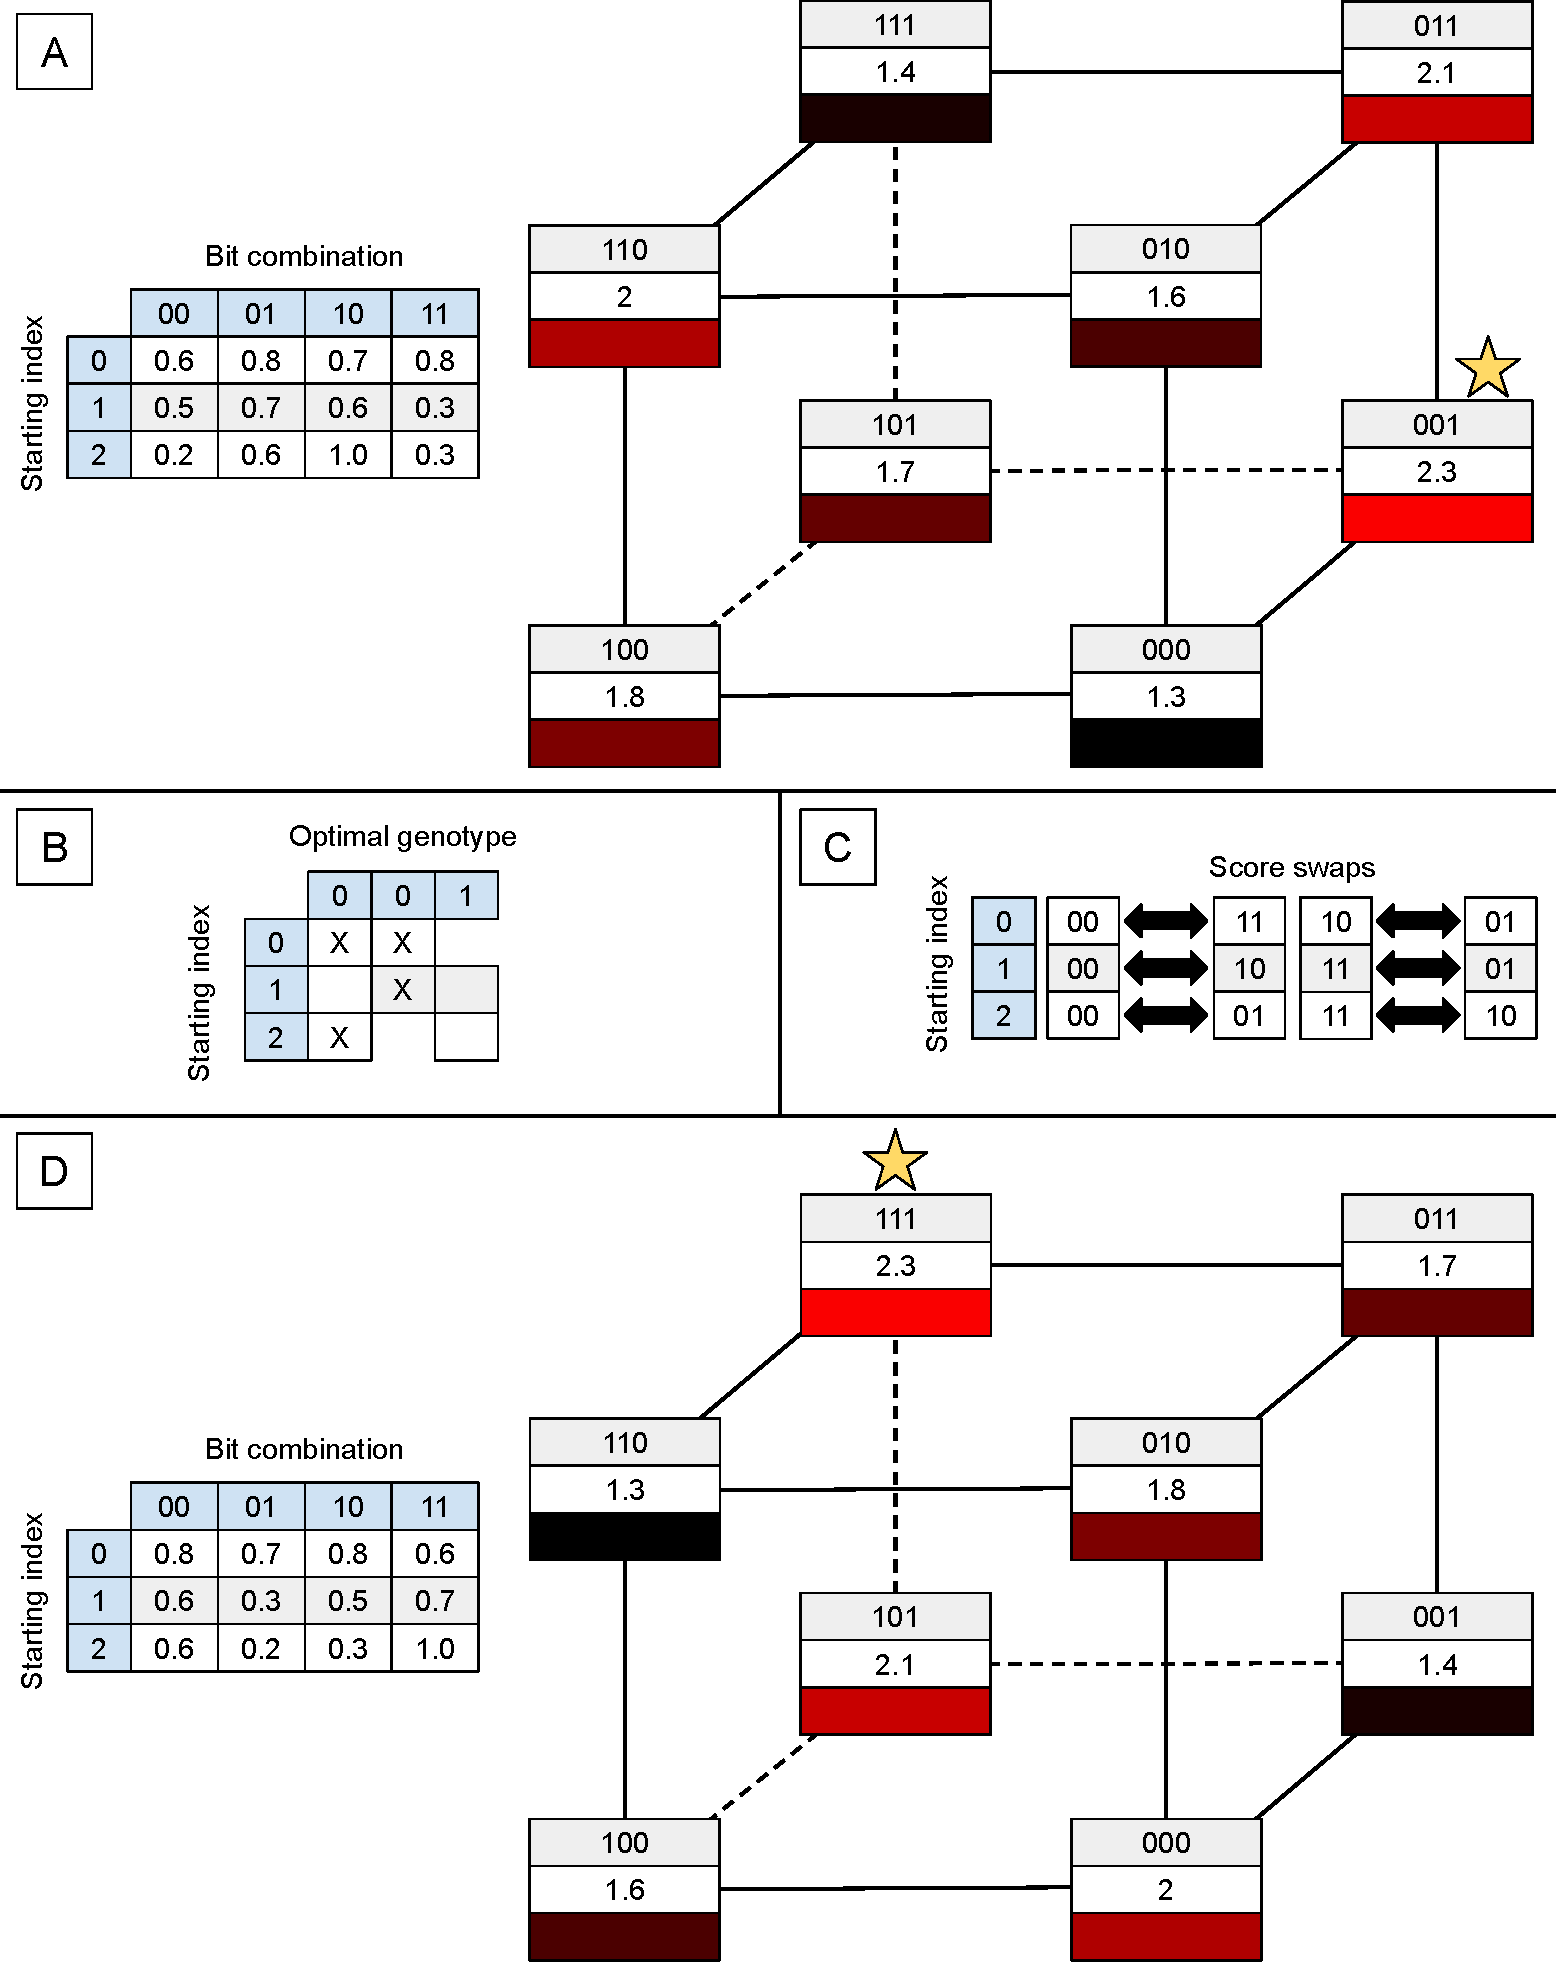
\includegraphics[width=0.9\textwidth]{04_simplified_model/media/rotating_landscape.pdf}
%     \caption{
%         An example of rotating an NK landscape where $N=3$ and $K=1$. 
%         Panel A shows the original landscape, including the score table and the visualized landscape. 
%         The yellow star shows the genotype with optimal fitness, 001. 
%         Panel B shows the mask of which bits need flipped, in this case the first two. 
%         These flips are demonstrated in Panel C.
%         At the first starting index both bits are flipped, while only one bit is flipped in the other indices. 
%         Finally, Panel D shows the resulting score table and landscape, which is isomorphic to the first but now 111 has maximal fitness.
%     }
%     \label{fig:simplified_model:rotating_landscape}
% \end{figure}

% We make one change to the NK landscape to make our analysis easier. 
% Traditionally in bitstring models, the distance between two bitstrings is calculated as their Hamming distance.
% To make comparisons with the global optimum easier, we propose to ``rotate'' the NK landscape. 
% Once the global optimum is known (in this case, found via brute force enumeration), the scoring rules of the landscape can be changed such that the global optimum occurs at the bitstring of all ones. 
% To accomplish this, for every zero in the original global optimal bitstring, we must swap the scores anywhere this bit is used. 
% This does not change the topology of the landscape, it merely re-labels the genotypes within.
% Figure \ref{fig:simplified_model:rotating_landscape} shows an example 
% Note that this is equivalent to XOR-ing a bitstring with the complement of the global optimum bitstring before evaluating its score.
% Once this transformation is complete, the distance to the optimal, successful, genotype is simply the number of zeros in a genome. 

I will conduct evolution like a traditional synchronous-generation genetic algorithm. 
I will seed the initial population of bitstrings with the genotype being tested, and evaluate each bitstring on the landscape. 
After this evaluation, I will select parents via a mix of elite selection (to ensure the optimal genotype persists if it is discovered) and tournament selection. 
Finally, all parents will be copied and possibly mutated, creating the next generation to be evaluated. 
I will then repeat this process until a stopping criterion is met. 

Quantifying the potentiation of a genotype is done by seeding some number of evolutionary replicates with that genotype and measuring the percentage of those replicates that evolve the target trait (as originally introduced in \citet{blountHistoricalContingencyEvolution2008}). %the percentage of replicates that evolve the target behavior when starting at that genotype. 
Typically, this is only measurable via multiple replay experiments that restart evolution at specific points along a lineage. 
Because I am using bitstrings, I am able to enumerate potentiation for \textit{all} possible genotypes in a landscape, creating a ``potentiation landscape''. 
This requires nontrivial effort, as there are $2^{N}$ possible genotypes in an $N$-length bitstring, and analyzing each genotype requires multiple evolutionary replicates started from it (here I use 50). 
%Once the 50 replicates for a given genotype are finished, I calculate potentiation as the percentage of those replicates evolved the target trait. 
%For the first time, we will be able to observe how potentiation changes with every step, both along a lineage and in the neighboring steps that could have been taken. 
This approach limits the size of landscapes that I can enumerate. 
As such, I propose to start by analyzing landscapes where $N \in \{10,12,14,16\}$ bits.
For each of these $N$ values, I will also vary $K \in [0, N - 1]$.
To ensure we observe the diversity landscapes can have at a particular combination of $N$ and $K$, I will enumerate the potentiation landscape for 30 landscapes at each pair of values. 

% First, we define the patterns of potentiation that we hope to observe in the system. 
% These are refined from the exploratory work of Chapter \ref{chap:replaying_associative_learning}, and are subject to change as we finish Chapters \ref{chap:replaying_associative_learning} and \ref{chap:varying_environments}.
% The three types of potentiation are: 
% \begin{enumerate}
%     \item Mutating toward the behavior, reducing the number of mutations to get there in the future
%     \item Shifting toward another genotype with the behavior that has a larger fitness advantage
%     \item Moving to another point in the genotype space such that the path toward the behavior becomes easier to traverse
% \end{enumerate}
% The three types of potentiation are visualized in Figure \ref{fig:06:conceptual_figure}

% We have constructed a bitstring model that allows for all three types of potentiation. 


% \begin{figure}
%     \centering
%     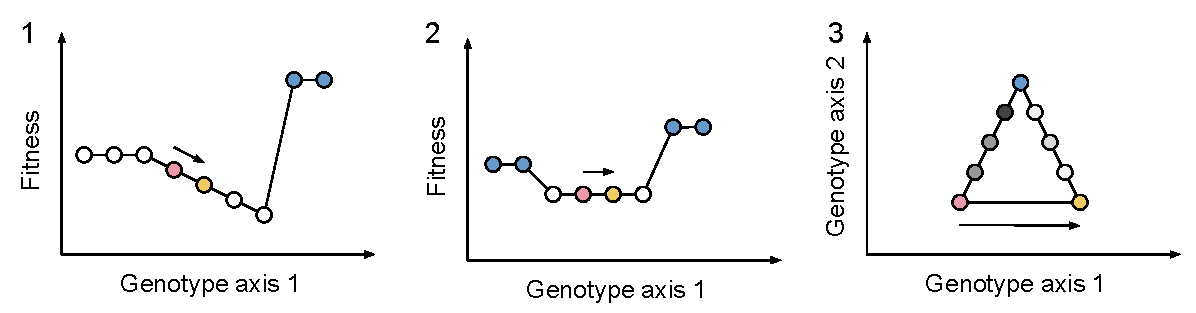
\includegraphics[width=0.9\textwidth]{04_simplified_model/media/potentiation_types_conceptual_figure.pdf}
%     \caption{
%     A conceptual figure demonstrating the three types of potentiating mutations.
%     The first two subplots show fitness on the y-axis, while the final subplot requires two genotype-space axes. 
%     All plots show the starting genotype in red, the potentiated mutant in yellow, and one or more genotypes with the focal trait in blue.
%     Arrows also show the mutation. 
%     The final subplot shows fitness of intermediate points on a grayscale axis with lighter colors being more fit.}
%     \label{fig:06:conceptual_figure}
% \end{figure}

\subsection{Proposed comparative analyses}

I plan to conduct two comparisons of potentiation: one between the NK landscape and the associative learning Avida domain, and the other across different $N$ and $K$ values within the NK landscape. 
However, the measurements taken in the associative learning domain were looking at potentiation along a lineage, not over the entire landscape (see \ref{sub:potentiation_measures} for the list of measurements). 
I will calculate the lineage metrics in the NK landscape by rerunning replicates at particular genotypes, tracking the evolving phylogenies. 
Specifically, I will target genotypes with low potentiation values, below 10\%, in order to create a fair comparison with the low initial potentiation seen in the associative learning results. 
Here, however, we do not need to perform replay replicates along these lineages, as we already know the potentiation of every possible genotype.
We merely need to map genotypes along the lineage with their potentiation values. 
Once potentiation has been assigned to every genotype along the lineage, we can calculate the potentiation measurements as normal. 

After these measurements have been collected, I will compare the distributions of each with those found in the associative learning environment of Chapter \ref{chap:replaying_associative_learning}.
As an example, I will test if there is a significant difference in the largest single-step potentiation gain between the two systems. 
Not all measurements translate to this system, but largest single-step potentiation gain/loss, the distance to the target trait from the potentiating mutations, and distributions of fitness effect apply equally to both systems. 
This will provide the first comparison of potentiation across environments and representations. 
If the distributions are similar, that would be strong evidence that there are general trends in potentiation. 
If, instead, significant differences exist, that will also provide information on what our simplified model might be missing. 

Next, I plan to perform a similar analysis across $K$ values in the NK landscape. 
Since $K$ controls the level of epistasis in the landscape, these tests will highlight the effect that epistasis has on our potentiation measurements. 
I will perform this analysis for each of the $N$ values tested. 
I will compare the relevant potentiation measurements across the set of $K$ values, seeing which ones statistically differ. 
%For example, does the fitness effect of potentiating mutations change as we increase the level of epistasis in the system? 
For example, I expect increased epistasis to make the landscapes more deceptive and thus increase the effect size of potentiating mutations.
Likewise, I will examine the consistency of the effect of $K$ on potentiation, by comparing fixed $K$ values across each $N$.

For both of these comparisons, I will conduct a Kruskal-Wallis test across all groups to see if any significant difference is found \citep{kruskal_use_1952}. 
If a difference is present, I will then conduct pairwise Mann-Whitney-Wilcoxon tests to determine which pairs of groups differ \citep{10.2307/3001968}.
Finally, I will apply Holm-Bonferroni corrections for multiple comparisons where needed \citep{holmSimpleSequentiallyRejective1979}.

% I propose a set of analyses that expand upon the work proposed in Chapter \ref{chap:replaying_associative_learning}. 
% Overall, I will enumerate multiple landscapes for various values of $N$ and $K$, calculating potentiation for every possible genotype. 
% This will allow us to compare the fitness landscape with the ``potentiation landscape'' for the first time. 
% As such, we can examine the relationships between fitness, potentiation, the distance to the target genotype, $N$, and $K$.
% Additionally, in enumerating genotype space, we will be running multiple evolutionary replicates from each genotype. 
% We can examine the dominant lineage of any of these replicates, allowing us to see how potentiation changed over time. 
% This allows us to compare potentiation in this system to that of Chapter \ref{chap:replaying_associative_learning}, which looked at the potentiation of associative learning in Avida. 

% To map the potentiation landscape, I will quantify potentiation at every possible genotype. 
% In our bitstring model, that can be accomplished by testing every bitstring in $[0, 2^{N} - 1]$.
% For a given genotype, we measure potentiation in the same way as previous work \citep{blountHistoricalContingencyEvolution2008} (Chapter \ref{chap:alife_submission}); we run a large number of evolutionary replicates starting from that genotype and calculate the percetange of those replicates that evolve the target trait. 
% This has traditionally been done along a lineage, but the same test holds for arbitrary genotypes. 
% The one difference is the time allowed in those evolutionary replicates. 
% Along a lineage, time is typically controlled such that the number of generations before that time point is subtracted from a total generation budget, ensuring that genotypes later in the lineage see fewer generations than those earlier. 
% Here we simply give all genotypes the same budget of 5,000 generations, which should be more than enough to traverse stable point. 
% I will perform these enumerations on 50 landscapes per treatment, varying $N \in [10,16]$ and $K \in [0,4]$ for a total of 35 treatments and 1750 landscapes. 
% This requires substantial computation effort, but preliminary experiments show that a 10-bit landscape can be fully enumerated in a matter of hours (a comparable amount of time to one initial replicate in Chapter \ref{chap:alife_submission}).

% Once the landscapes have been enumerated, I will analyze the relationships within and between treatments. 
% Within a treatment (a combination of $N$ and $K$), I will examine the distributions of potentiation of all genotypes.
% A Kruskal-Wallis test will determine if any significant variation exists among these distributions \citep{kruskal_use_1952}. 
% In each treatment, I will also inspect the relationship between fitness and potentiation for a sampling of landscapes. 
% I hypothesize that low potentiation can arise from populations reaching a local optima, preventing them from reaching the global optimum because valley crossing would be required. 
% If this is the case, I expect to see a negative correlation between the fitness and potentiation. 
% However, due to the nature of NK landscapes, I also expect points close to the global optimum to also have high fitness, while also having high potentiation. 
% As an illustrative example, think of all $N$ genotypes that are one step away from the global optimum; these genotypes are likely to have high fitness (though not guaranteed), however, they are guaranteed to have lower fitness than the global optimum and thus a very high potentiation. 
% As such, I expect \textit{many} genotypes to experience a negative correlation between fitness and potentiation, but with exceptions in genotypes that are close to the global optimum and have a path of ever-increasing fitness to that optimum. 
% Because the number of possible direct paths to the optimum increases factorially with distance to the global optimum, I will inspect these data with respect to their distance to the optimum. 
% I expect to see the negative correlation between fitness and potentiation to break down for short distances. 

% In calculating these potentiation values, I will be running evolutionary replays. 
% We can pull the dominant lineage of any of these replays to look at how potentiation changes throughout the lineage. 
% However, unlike previous work, we do not need to calculate the potentiation for the lineage, as we will know the potentiation for every possible genotype. 
% One important difference between this system and Avida is that these NK landscapes have no concept of a ``default ancestor''. 
% This means we do not have a single starting genotype from which we can observe how potentiation changes over different lineages. 
% Instead, we can sample successful lineages of genotypes that evolved the target trait from genotypes that have intermediate potentiation. 
% Genotypes that have 0\% or 100\% potentiation are not of interest, but all other values potentially are. 
% Specifically, I will sample lineages from genotypes with potentiation between 2\% and 15\% so they are comparable to those in Chapters \ref{chap:alife_submission} and \ref{chap:replaying_associative_learning}. 

% Once these lineages have been identified, I will collect the same potentiating measurements described in Section \ref{sub:potentiation_measures}. 
% I will then conduct statistical comparisons between the two systems. 
% As an example, I will test if there is a significant difference in the largest single-step potentiation gain between the two systems. 
% Not all measurements make sense in this system, but largest single-step potentiation gain/loss, the distance to the target trait of potentiating mutations, and distributions of fitness effect apply equally to both systems. 
% This will provide the first comparison of potentiation across environments and representations. 
% If the distributions are similar, that would be strong evidence that there are general trends in potentiation. 
% If, instead, significant differences exist, that will also provide information on what our simplified model might be missing. 

\subsection{More advanced analyses} 

Finally, there are some analyses that are tractable in the NK landscape that were infeasible in Avida.
Indeed, the power of being able to generate a potentiation landscape suddenly makes many additional analyses possible. % allows many additional analyses to suddenly become possible.
Local optima can be counted in the NK model, allowing me to investigate the relationship between potentiation and the number of local optima in the landscape. 
Similarly, the enumeration of both the fitness and potentiation landscapes will allow me to examine correlations between potentiation and fitness for individual genotypes. 
Due to local optima, I expect potentiation to decrease with fitness, but I also expect this distribution to be bimodal as genotypes close to the global optimum should have both high fitness and high potentiation. 
For any optimum, we can determine the set of genotypes that have a path to that optimum that monotonically increases in fitness (i.e., the basin of attraction for that optimum \citep{ostmanPredictingEvolutionVisualizing2014}). 
We can then see if crossing into the set of genotypes that have a path to the global optimum increases potentiation. 
However, the global optimum entering that set may not be enough; we may not see jumps in potentiation until the we reach a genotype where \textit{only} the global optimum is in that set.
%I expect that mutating to a genome that \textit{only} includes the global optimum in that set to maximize potentiation. 

In Chapter \ref{chap:alife_submission}, I inspected the two-step mutational neighborhood in an attempt to identify how potentiating mutations interacted with the target trait. 
The limited scope of that analysis brings its usefulness into question. 
In this NK landscape, however, we can exhaustive examine each genotype in its relationship to the local mutational neighborhood. 
This will allow me to investigate how often changes to the $n$-step mutational neighborhood translate to meaningful differences in potentiation. 
We can calculate the fraction of $n$-step mutants that are both beneficial and closer to the target trait. 
%This is effectively testing the level of epistasis up to $N$ steps out. 
How well does this correlate with potentiation? 
If we see that increasing this fraction for one- and two-step neighbors correlates well with potentiation, then this may be useful in more complex systems. 
If there is no strong signal, then this analysis may not be worth continuing in the future. 
%Analysis of the mutational neighborhood, as in Chapter \ref{chap:replaying_associative_learning}, also becomes much easier in the NK landscape. 
%This allows me to see how potentiating mutations effect the distance to the global optimum. 

%By leveraging search algorithms, 
I will also test if the probability of the most likely path from a given genotype to the target trait is a strong indicator of potentiation. 
By enumerating the fitness landscape, I can compare the fitness between one genotype and all $N$ of its one-step mutants. 
Assuming a mutation occurs, I can use the fitness values of each mutant to create the probability that each mutation would be selected (this varies with several factors, such as the selection scheme in use). 
By doing this for every genotype, I can create a graph of the entire genotype space with genotypes as nodes and their transition probabilities as weighted edges. 
Next, I will perform a negative log transformation on each weight. 
This will transform the probabilities into positive values, with smaller probabilities converting to larger values. 
Due to the nature of logarithms ($log(ab) = log(a) + log(b)$), summing these log-transformed values is the equivalent to multiplying the underlying probabilities. 
As such, this approach allows us to perform a search from a given genotype to the target trait using Dijkstra's algorithm. 
This analysis will return the \textit{most likely} path through genotype space to get from that genotype to the target. 
I will calculate this value for each genotype, and then analyze its relationship with potentiation. 
Since multiple adaptive paths between a genotype and the target can exist, I expect that, in many cases, this measure fails to accurately predict potentiation. 
Future work can then expand on this analysis by finding the $k$ shortest paths to the target trait, and seeing how many paths are required to accurately approximate potentiation \citep{eppsteinFindingShortestPaths1998}. 


\subsection{Broader impacts}

%This work has the potential to provide evidence for or against patterns in potentiation across systems. 
This work will be the first empirical measure of patterns in potentiation across systems.
Compared to Chapter \ref{chap:replaying_associative_learning}, if we see similar patterns in potentiation, then we can start to consider that these patterns may be generally applicable, at least in digital evolution but potentially into natural systems. 
If not, we can dive into the differences in patterns to begin asking if other systems will be more like one system or the other. 
Additionally, this work will provide insight into how we measure potentiation and characterize potentiating mutations, and these landscapes will provide a second data set for future comparative studies. 

% Talk about how we can explore our intuition and approximations of potentiation in this system?

If I find evidence of interesting potentiation dynamics in this system, that will help establish NK landscapes as a useful tool for investigating potentiation. 
An NK landscape where $K = 0$ is just a single hill to climb, and as such I expect all genotypes in that landscape to have 100\% potentiation. 
If I see potentiation vary more across landscapes as $K$ increases, that will provide support for the hypothesis that epistatic interactions are key to potentiation. 
They might not be the only factor though, and future models may need to expand beyond the traditional NK model. 
If, for instance, I do not see large jumps in potentiation, I may need stronger binary ``on/off'' forms of potentiation. 
A simple example would be a bitstring environment where the first half of the bitstring is evaluated on one NK landscape and the second half on another, with the target trait being optimal genotypes in both landscapes. 
If I limit fitness such that the second half of the bitstring only contributes to fitness if the first half is at the global maximum, then I would expect to see a drastic increase in potentiation when the first half reaches that optimal genotype. 
This model would more directly simulate required building blocks in the evolution of the target trait. 
There are many ways that we could extend the traditional NK model, and this work will help shape those future studies, if needed. 

\section{Preliminary results}

To ensure that potentiation in NK landscapes is not entirely trivial, I ran some very early preliminary data. 
I selected $N=10$ and enumerated potentiation in 50 landscapes each of $K \in \{0,1,2,3\}$.
For each landscape, I ran 50 replicates from every genotype (1,024 genotypes per landscape) to quantify potentiation at that point. 
%These data are not fully analyzed and these plots are rough, this was last-minute data to make sure this environment was worth looking into. 

\begin{figure}[h!]
    \centering
    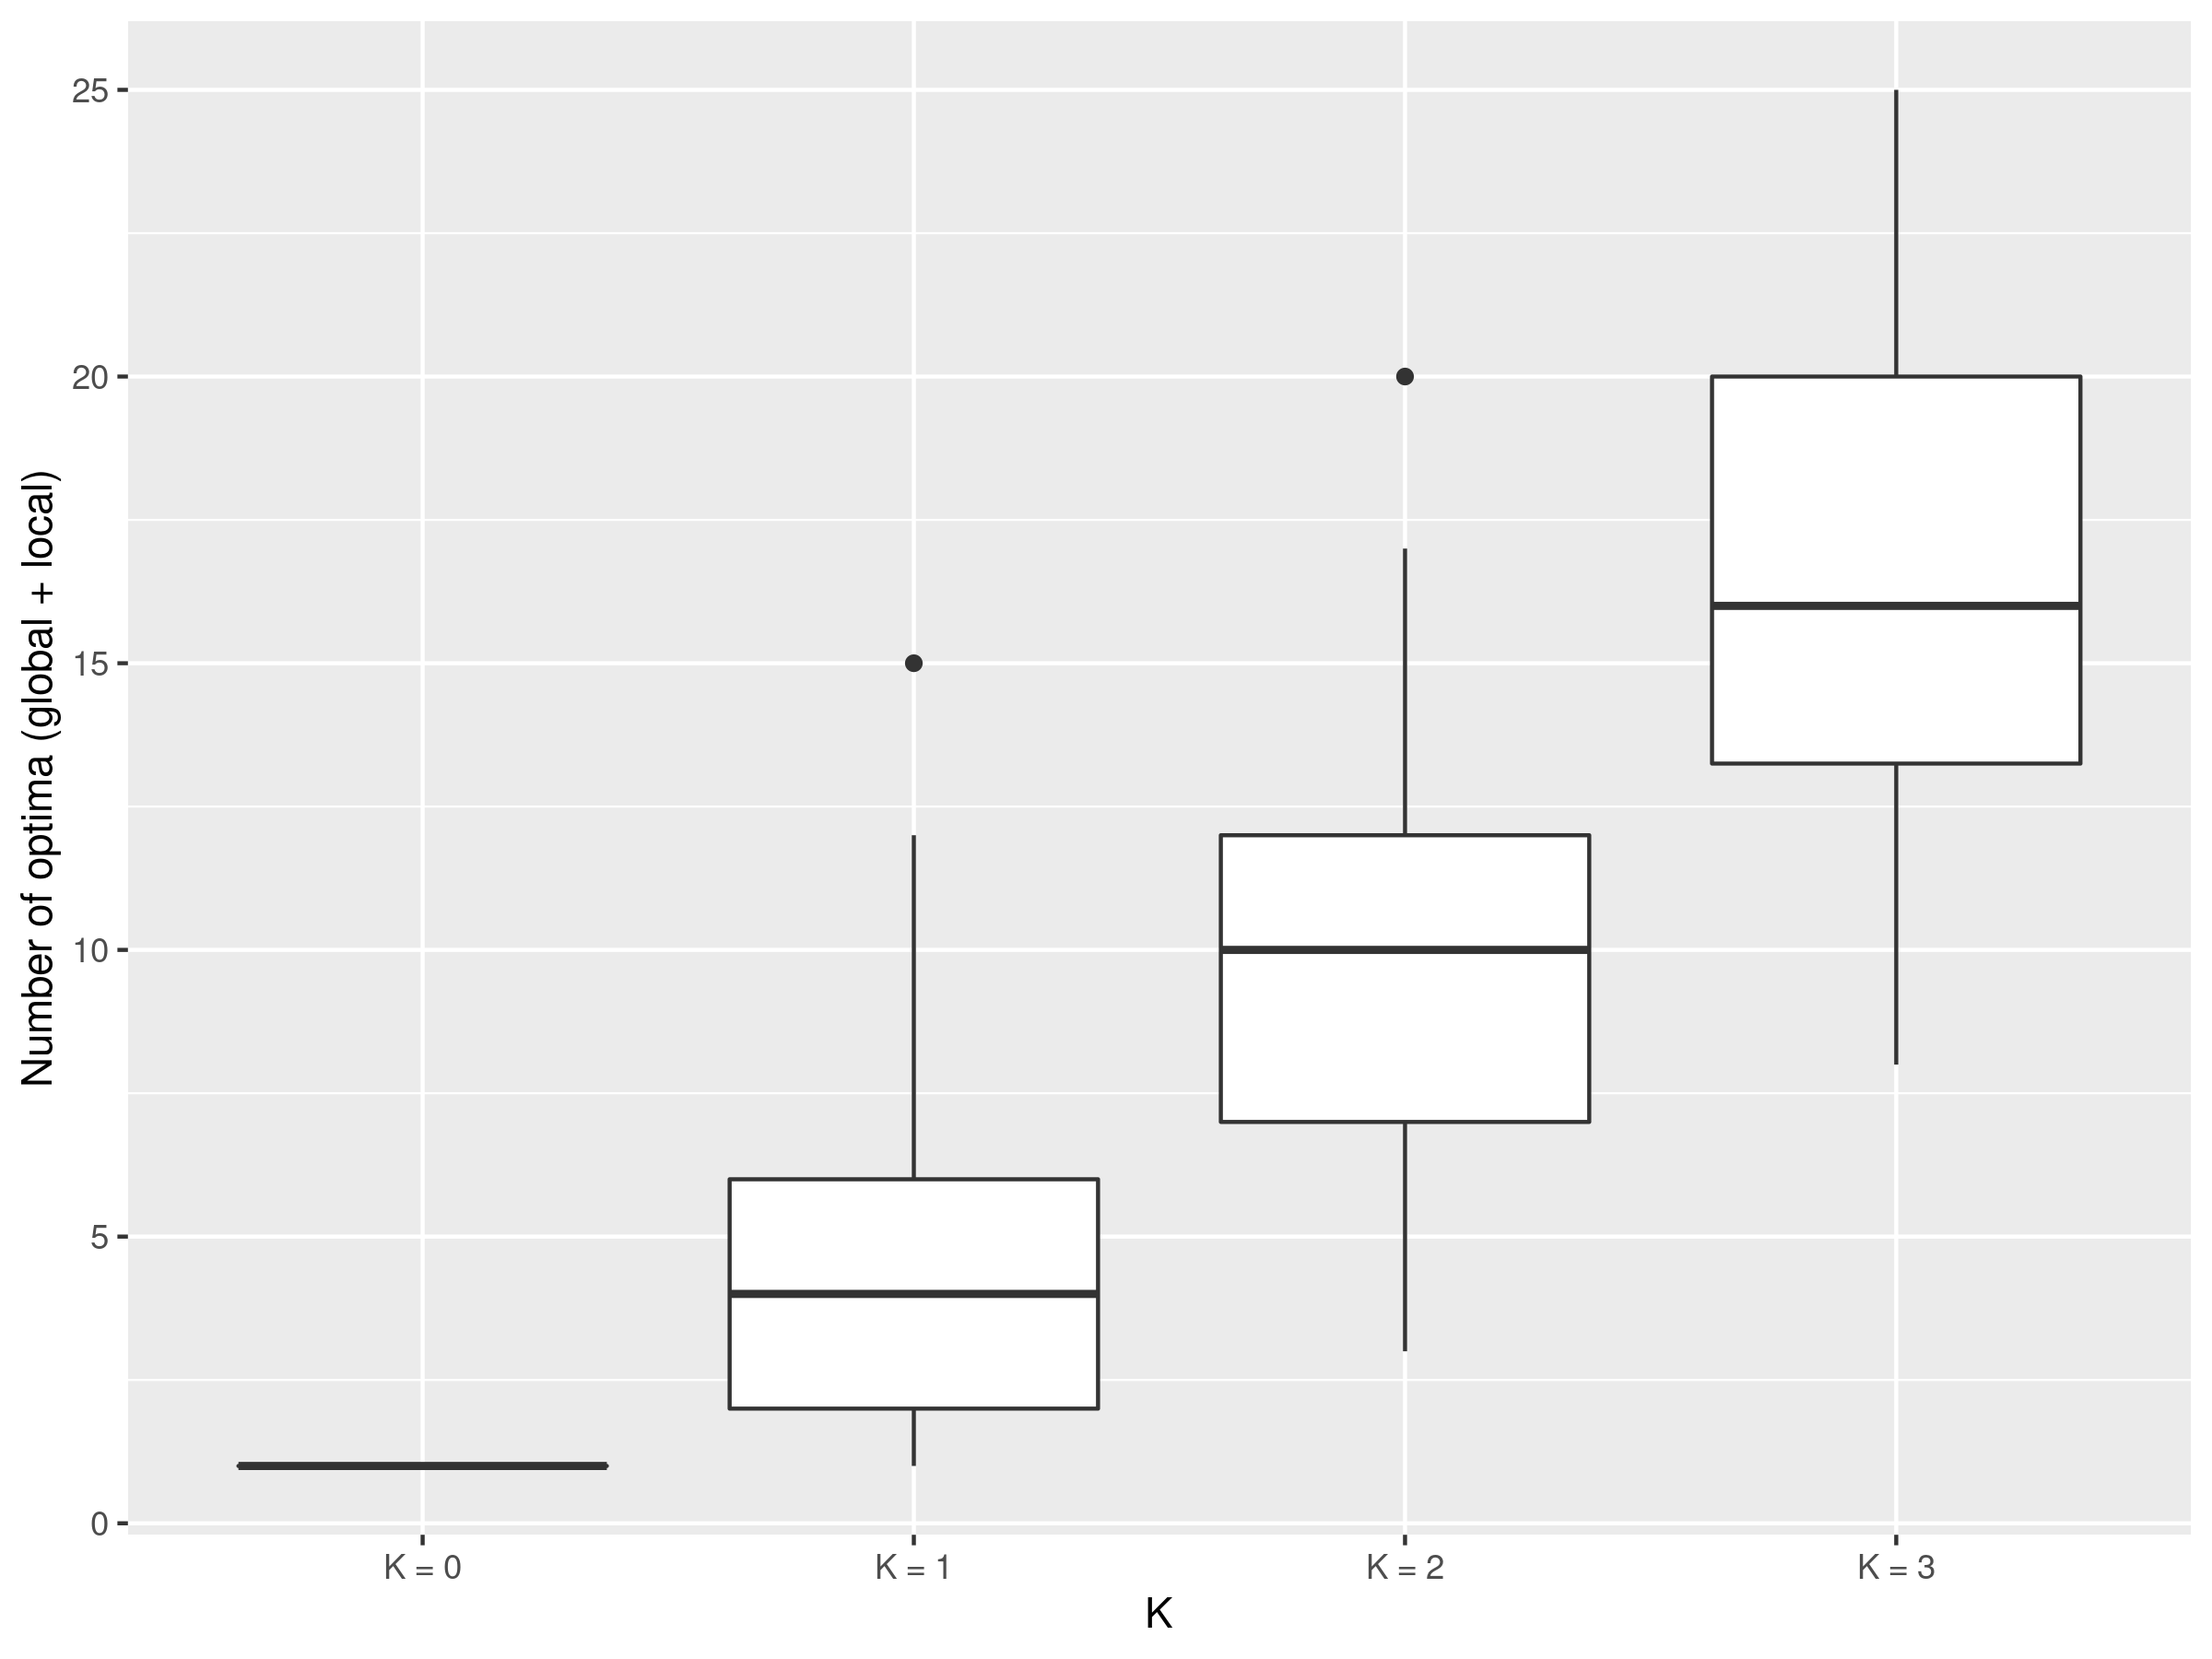
\includegraphics[width=0.95\textwidth]{04_simplified_model/media/num_peaks.png}
    \caption{
        Boxplots showing the number of peaks in all 50 landscapes of a given $K$ value. 
    }
    \label{fig:simplified_model:num_peaks}
\end{figure}

First, Figure \ref{fig:simplified_model:num_peaks} shows the number of peaks at each $K$ value. 
Here we define a peak as a genotype that has higher fitness than the $N$ genotypes around it; this definition includes local optima as well as the global optimum \citep{ostmanPredictingEvolutionVisualizing2014}. 
NK landscapes are often described as ``tunably rugged'', with larger $K$ values creating more rugged landscapes due to increased epistatic interactions. 
We see exactly that here, as the number of peaks increases smoothly as we increase $K$. 

\begin{figure}[h!]
    \centering
    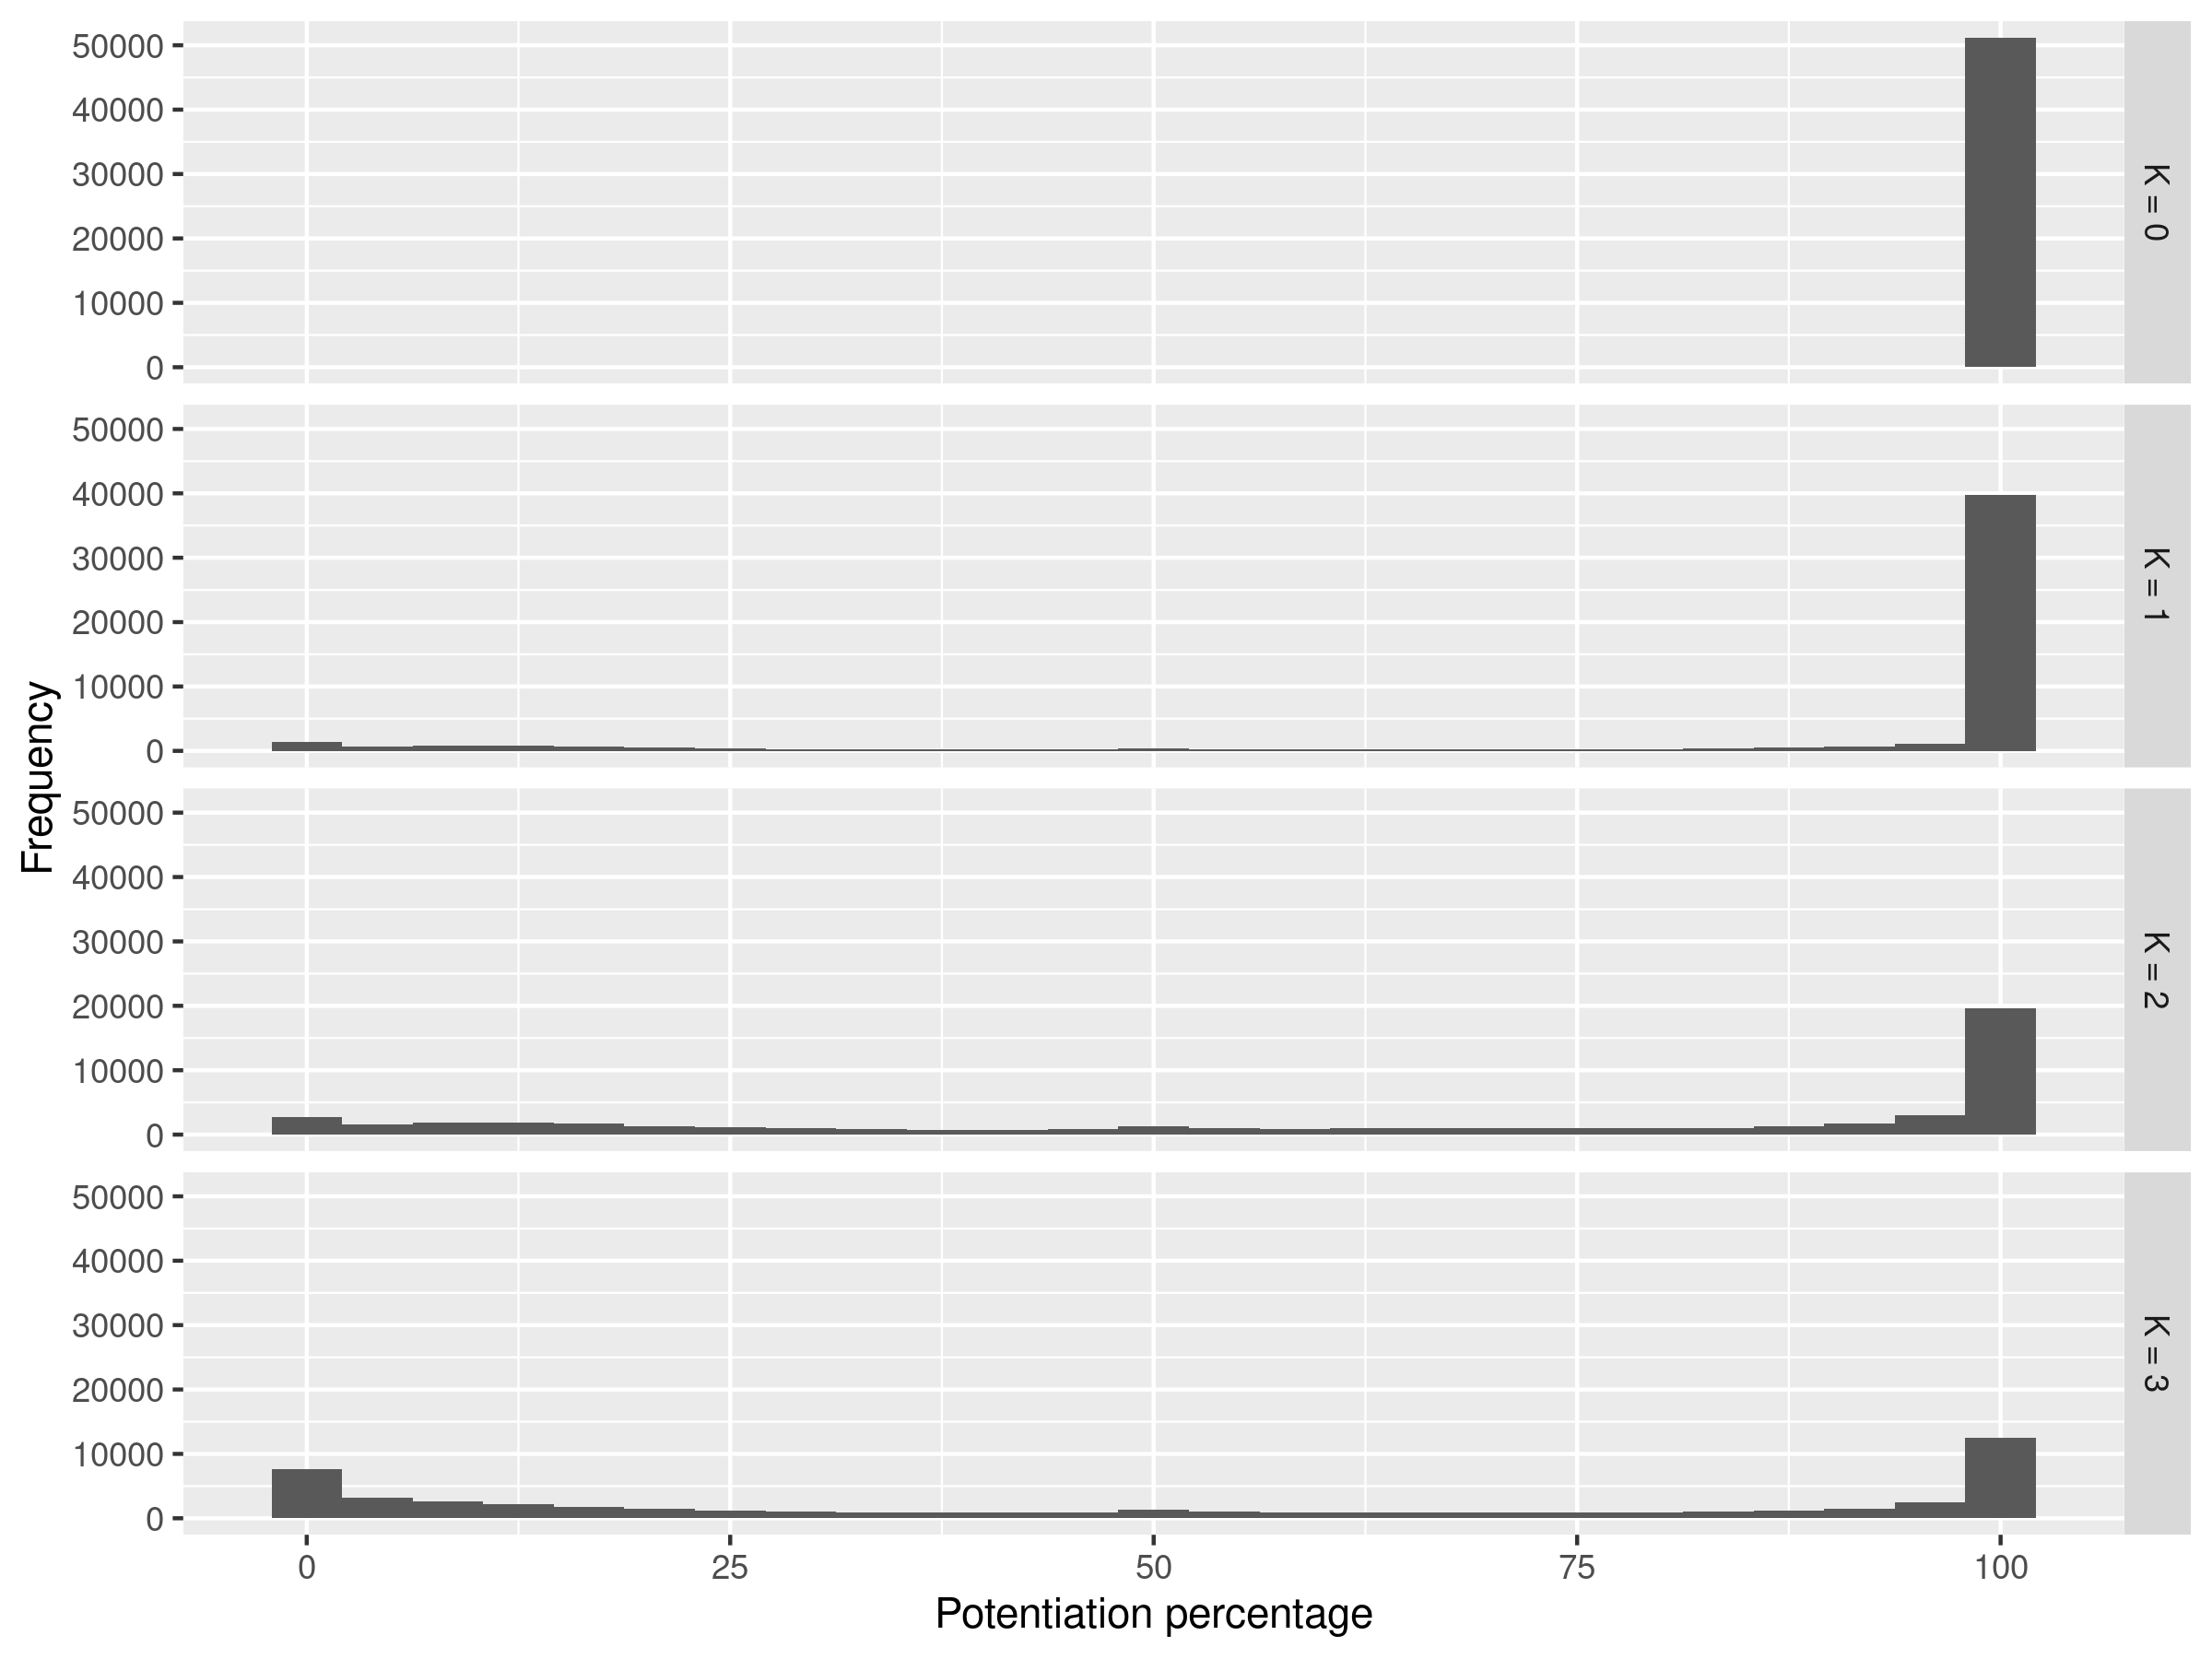
\includegraphics[width=0.95\textwidth]{04_simplified_model/media/success_histogram.png}
    \caption{
        Histograms of potentiation, with one row per $K$ value.
        Each histogram includes the potentiation of all 1,024 genotypes in all 50 landscapes for that $K$ value.
    }
    \label{fig:simplified_model:potentaition_histogram}
\end{figure}

Figure \ref{fig:simplified_model:potentaition_histogram} shows the overall distribution of potentiation across all genotypes in all landscapes at each $K$ value. 
First, $K=0$ shows 100\% potentiation for every genotype in every landscape, which matches expectations as individual bits can be optimized independently (i.e., there is zero epistasis) and thus the landscape is a single hill to climb. 
As $K$ increases, we see some mass of the distribution shift from 100\% potentiation to the lower values, especially the very low values around 0\%. 
This also meets my expectation, as we have shown that increasing $K$ increases the number of local optima and thus creates more opportunities for populations to become ``stuck'' and unable to reach the global optimum. 
When it comes time to compare potentiation in this model to that in Avida, we do see genotypes with potentiation levels similar to those found in Avida, indicating that we can conduct those comparisons fairly. 

\begin{figure}[h!]
    \centering
    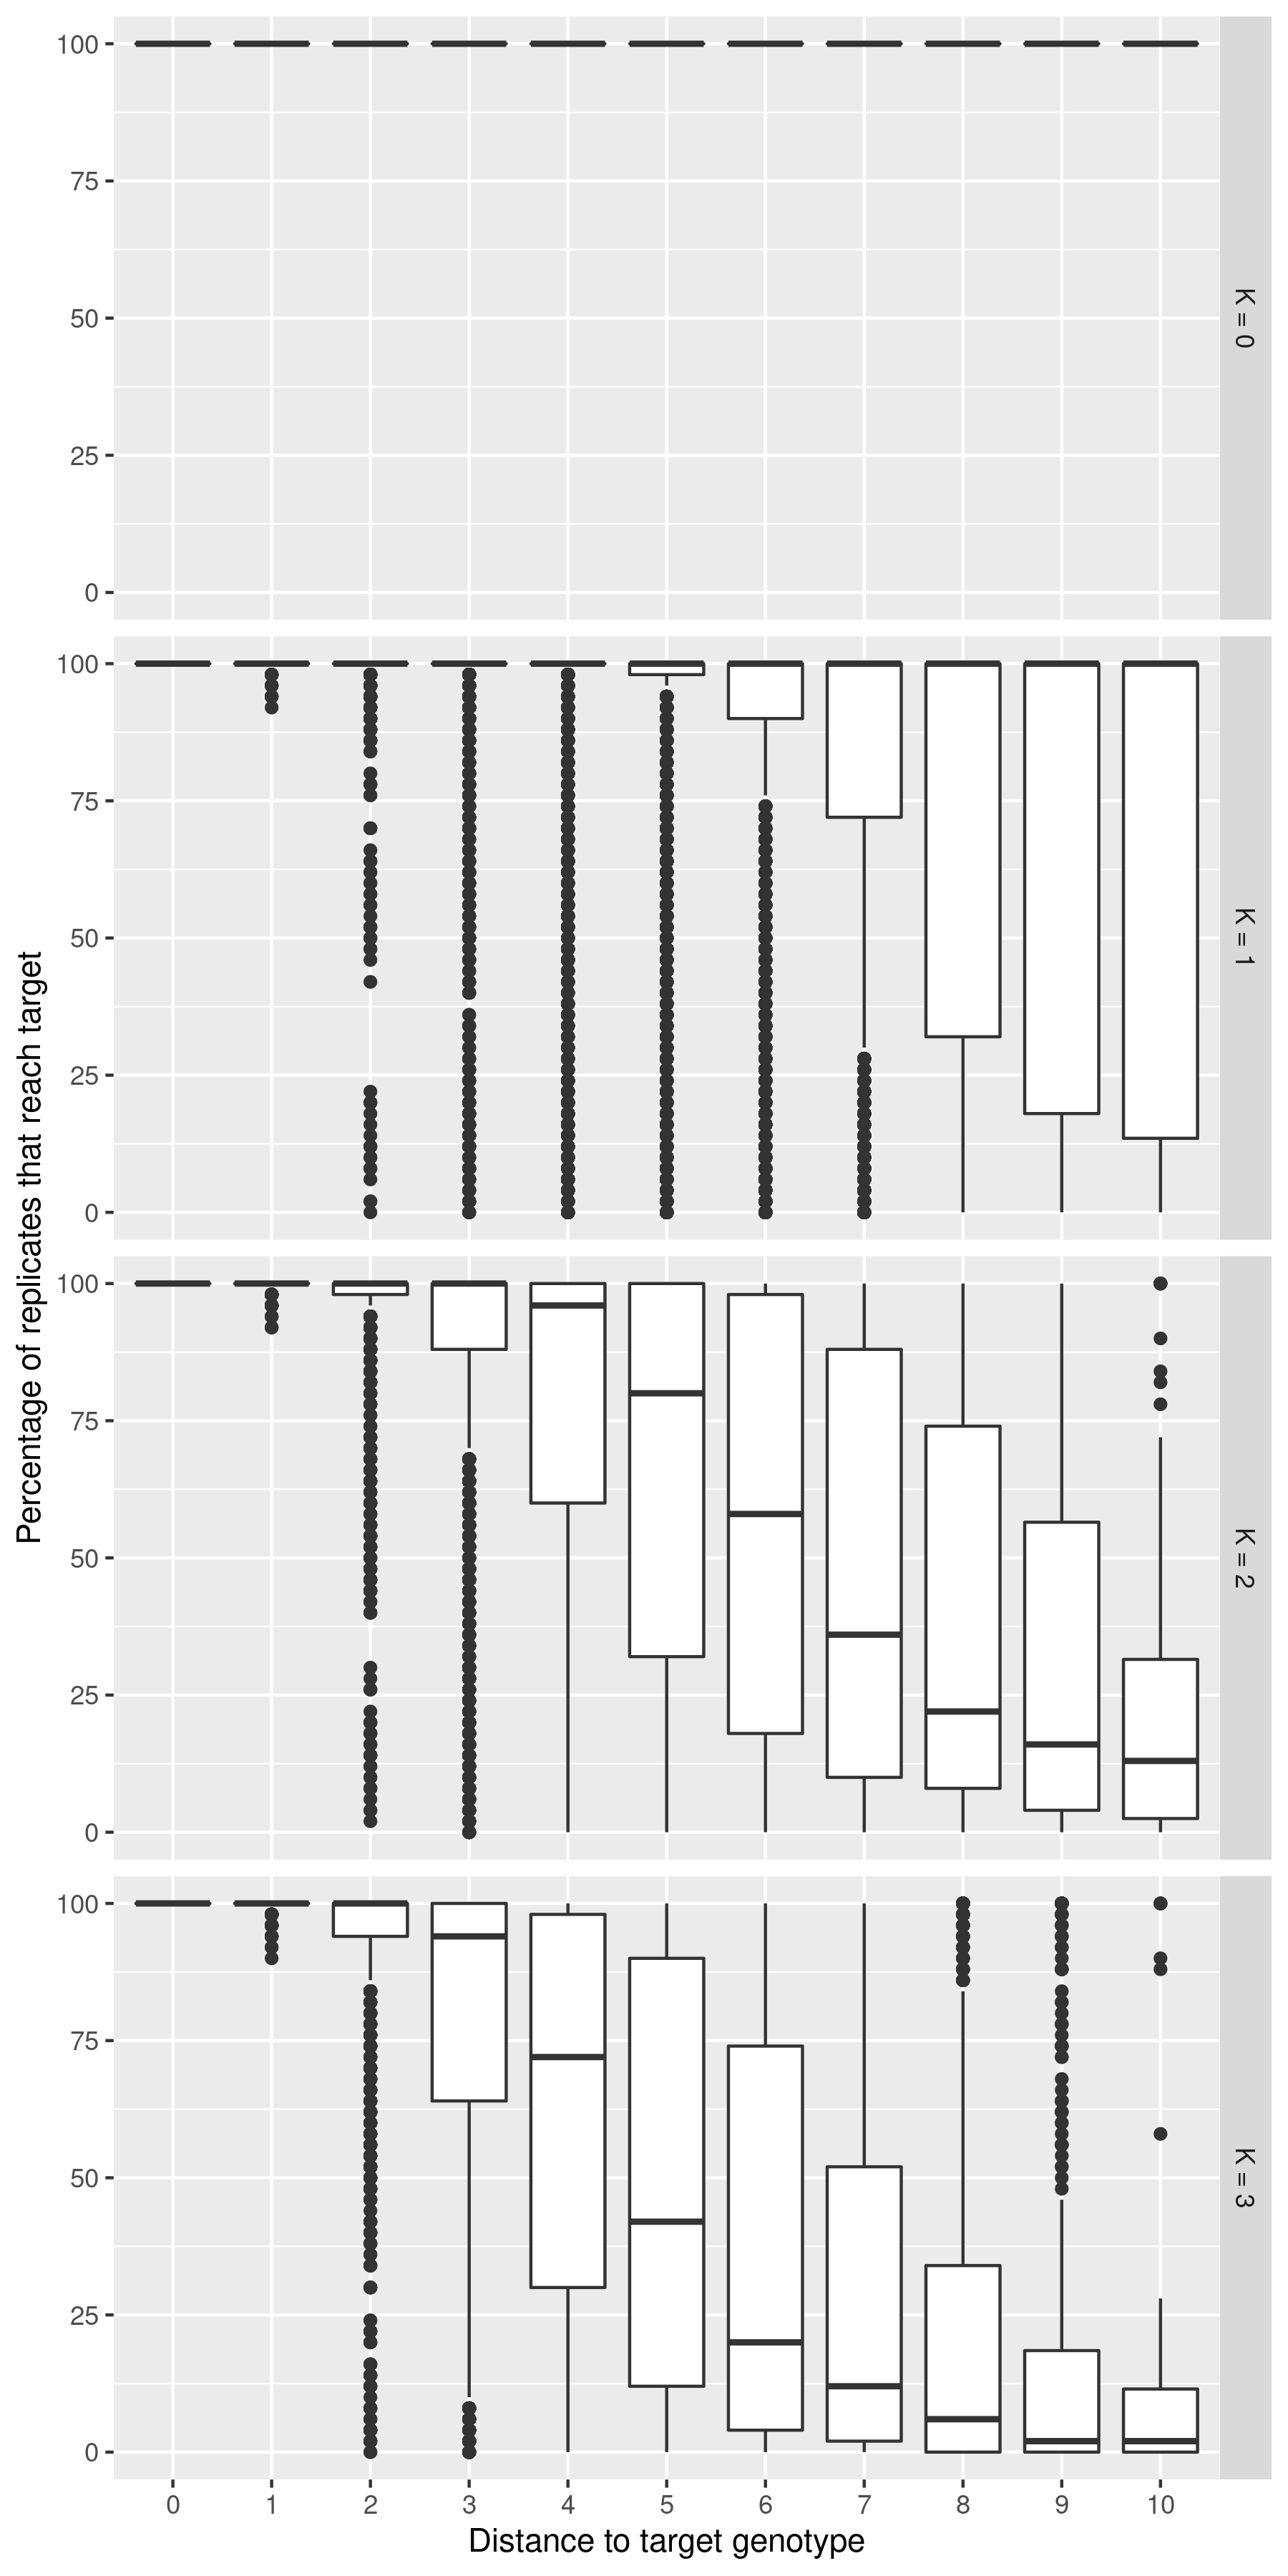
\includegraphics[width=0.6\textwidth]{04_simplified_model/media/potentiation_by_distance_boxplots.png}
    \caption{
        Boxplots showing the potentiation of genotypes at a given distance away from the global optimum. 
        Rows show the various $K$ values, and each boxplot shows all genotypes at that distance for all 50 landscapes for that $K$ value. 
    }
    \label{fig:simplified_model:distance_boxplots}
\end{figure}

Finally, Figure \ref{fig:simplified_model:distance_boxplots} shows how potentiation changes as we vary $K$ and look at the distance from a genotype to the target trait.
As we have already seen, $K = 0$ is a single hill and thus all genotypes are fully potentiated. 
Starting at $K=1$, we see that while the median potentiation stays consistently high, the lowest quartile decreases as distance from the target increases. 
At $K=2$, we see the whole distribution of potentiation shift to lower values as distance increases, with very few points at the maximum distance having high potentiation. 
This trend continues into $K = 3$, becoming more pronounced. 
Overall, Figure \ref{fig:simplified_model:distance_boxplots} meets my expectations. 
In the simpler landscapes, most genotypes have high potentiation, but as the landscapes become more rugged we see potentiation fall faster as we increase the distance to the target. 

While these data are only a shallow glance into potentiation in NK landscapes, they provide reassurance that the system is worthy of examination. % looking into.
When performing the work in earnest, I will be analyzing landscapes with higher values of $N$ and $K$. %, and performing deeper analyses by looking at aspects such as the basins of attraction to the target.
Additionally, I will be looking at the lineages of semi-potentiated genotypes, allowing me to compare the potentiation measures that will be recorded in Chapter \ref{chap:replaying_associative_learning}. 
This brief glimpse reveals promise in the system; hopefully this promise holds true and NK landscapes can help us delve further into potentiation. 
\chapter{Adaptive phenotypic plasticity
stabilizes evolution in fluctuating environments}
\label{chap:consequences_of_plasticity}

\noindent
Authors: Alexander Lalejini, Austin J. Ferguson, Nkrumah A. Grant, and Charles Ofria

\noindent
Note: This chapter is adapted from \citep{lalejiniAdaptivePhenotypicPlasticity2021}. 
The only change is the lead-in paragraph at the beginning. 


%%%%%%%%%%%%%%%%%%%%%%%%%%%%%%%%%%%%
% Utility commands
%%%%%%%%%%%%%%%%%%%%%%%%%%%%%%%%%%%%
%\newcommand{\code}{\texttt}

%%%%%%%%%%%%%%%%%%%%%%%%%%%%%%
% Evolutionary change rate experiment
%%%%%%%%%%%%%%%%%%%%%%%%%%%%%%
% data from experiment - 2021-02-08
\newcommand{\evolutionaryChangeRateReplicates}{100}
\newcommand{\evolutionaryChangeRatePlasticReps}{42}

%%%%%%%%%%%%%%%%%%%%%%%%%%%%%%
% Novel traits experiment
%%%%%%%%%%%%%%%%%%%%%%%%%%%%%%
\newcommand{\novelTraitsReplicates}{100}
\newcommand{\novelTraitsReward}{10\%}
\newcommand{\novelTraitsPlasticReps}{42}

%%%%%%%%%%%%%%%%%%%%%%%%%%%%%%
% Deleterious hitchhiking experiment
%%%%%%%%%%%%%%%%%%%%%%%%%%%%%%
% - 2021-02-05 -
\newcommand{\deleteriousHitchhikingReplicates}{100}
\newcommand{\deleteriousHitchhikingPlasticReps}{43}
\newcommand{\instPoisonMagnitude}{10\%}

%%%%%%%%%%%%%%%%%%%%%%%%%%%%%%
% Metric definitions
%%%%%%%%%%%%%%%%%%%%%%%%%%%%%%
\newcommand{\SweepsMetricName}{
Coalescence event count
}
\newcommand{\SweepsMetricDesc}{
Number of coalescence events that have occurred, which indicates the frequency of selective sweeps in the population.
}

\newcommand{\MutationCountMetricName}{
Mutation count
}
\newcommand{\MutationCountMetricDesc}{
Sum of all mutations that have occurred along a lineage.
}

\newcommand{\PhenotypicVolatilityMetricName}{
Phenotypic volatility
}
\newcommand{\PhenotypicVolatilityMetricDesc}{
Number of instances where parent and offspring phenotypic profiles do not match along a lineage.
}

\newcommand{\MutationalStabilityMetricName}{
Mutational robustness
}
\newcommand{\MutationalStabilityMetricDesc}{
Proportion of mutations (from the set of all possible one-step mutations) that do not change the phenotypic profile of a focal genotype. We also measured \textit{realized mutational robustness}, which is the proportion of mutated offspring along a lineage whose phenotypic profile matches that of their parent.
}

\newcommand{\TaskPerformanceMetricName}{
Final novel function count
}
\newcommand{\TaskPerformanceMetricDesc}{
Count of unique novel functions performed by the representative organism in a final population from experiment \hyperref[sec:methods:exp:novel-task-evolution]{phase 2B}.
This metric can range from 0 to 71 and measures how well the fitness landscape was exploited  at a given point in time.
}

\newcommand{\TaskDiscoveryMetricName}{
Novel function discovery
}
\newcommand{\TaskDiscoveryMetricDesc}{
Number of unique novel functions ever performed along a given lineage in experimental \hyperref[sec:methods:exp:novel-task-evolution]{phase 2B}, even if a function is later lost.
This metric can range from 0 to 71 and measures a given lineage's level of exploration of the fitness landscape.
}

\newcommand{\TaskLossMetricName}{
Novel function loss
}
\newcommand{\TaskLossMetricDesc}{
Number of instances along a given lineage from experimental \hyperref[sec:methods:exp:novel-task-evolution]{phase 2B} where a novel function is performed by a parent but not its offspring.
This metric measures how often a given lineage fails to retain evolved traits over time.
}

\newcommand{\FinalPoisonMetricName}{
Final deleterious function count
}
\newcommand{\FinalPoisonMetricDesc}{
Number of times the deleterious function is performed by the representative organism from a final population from experiment \hyperref[sec:methods:exp:deleterious-instruction-accumulation]{phase 2C}.
}

\newcommand{\LineagePoisonMetricName}{
Deleterious function acquisition count
}
\newcommand{\LineagePoisonMetricDesc}{
Number of instances along a given lineage where a mutation causes an offspring to perform the deleterious function more times than its parent.
}


\begin{raggedbottom} 

%%%%%%%%%%%%%%%%%%%%%%%%%%%%%%%%%%%%%%%%%%%%%%%%%%%%%%%%%%%%%%%%%%%%%%%%%%%%%%%%%%%%%%%%%%
% INTRODUCTION
% The introduction should be succinct, with no subheadings.
%%%%%%%%%%%%%%%%%%%%%%%%%%%%%%%%%%%%%%%%%%%%%%%%%%%%%%%%%%%%%%%%%%%%%%%%%%%%%%%%%%%%%%%%%%

\section{Introduction}

%%%%%%%%%%%%%%%%%%%%%%
% COMPS-SPECIFIC LEAD IN
% Why does this fit in my dissertation? 
% Because it looks at the effect that early behaviors may have on future evolution
% In this case, if we want to understand cognitive behaviors (e.g., associative learning), we should think about what effects the potential building blocks may have. 
%%%%%%%%%%%%%%%%%%%%%%
When considering the role of history in evolution, we must consider what effects ``stepping stone'' behaviors may have on future evolutionary dynamics. 
In cognitive behaviors, these earlier milestones may take the form of reactive strategies that respond to environmental stimuli but do not store or integrate information. 
Here we investigate the evolution of one such reactive behavior: adaptively plastic metabolism regulation in a cyclic environment. 
In replicates that evolve the desired behavior, we use them to seed new replicates in a different environment, analyzing how the plastic behavior affects attributes such as novel function gain and the accumulation of deleterious traits. 
This work examines how the evolution of particular behavior can influence future dynamics, which could sway what other behaviors can later evolve. 

%%%%%%%%%%%%%%%%%%%%%%
% -- Different mechanisms evolve to cope with fluctuating environments, and those mechanisms
%    affect evolution. --
%%%%%%%%%%%%%%%%%%%%%%
Natural organisms employ a wide range of evolved strategies for coping with environmental change, such as
periodic migration \citep{winger_long_2019},
bet-hedging \citep{beaumont_experimental_2009},
adaptive tracking \citep{barrett_adaptation_2008},
and phenotypic plasticity \citep{ghalambor_adaptive_2007}.
The particular mechanisms that evolve in response to fluctuating environments will also shift the course of subsequent evolution \citep{wennersten_population-level_2012,schaum_plasticity_2014}.
As such, if we are to understand or predict evolutionary outcomes, we must be able to identify which mechanisms are most likely to evolve and what constraints and opportunities they impart on subsequent evolution.

%%%%%%%%%%%%%%%%%%%%%%
% -- We focus on how plasticity affects subsequent evolution. --
%%%%%%%%%%%%%%%%%%%%%%
In this work, we focus on phenotypic plasticity, which can be defined as the capacity for a single genotype to alter phenotypic expression in response to a change in its environment \citep{west-eberhard_developmental_2003}.
Phenotypic plasticity is controlled by genes whose expression is coupled to one or more environmental signals, which may be either biotic or abiotic.
For example, the sex ratio of the crustacean \textit{Gammarus duebeni} is modulated by changes in photoperiod and temperature \citep{dunn_two_2005}, and the reproductive output of some invertebrate species is heightened when infected with parasites to compensate for offspring loss \citep{chadwick_parasite-mediated_2005}.
% -- @AML: move next two lines to later as suggested by editor --
% In this study, we conducted digital evolution experiments to investigate how the evolution of adaptive phenotypic plasticity shifts the course of evolution in a cyclically changing environment.
% Specifically, we examined the effects of adaptive plasticity on subsequent genomic and phenotypic change, the capacity to evolve and then maintain novel traits, and the accumulation of deleterious alleles.


%%%%%%%%%%%%%%
% Effects of phenotypic plasticity on subsequent evolution disputed.
%   - baseline expections on rate of evolutionary response given adaptive vs. non-adaptive plasticity
%%%%%%%%%%%%%%
Evolutionary biologists have long been interested in how evolutionary change is influenced by phenotypic plasticity because of its role in generating phenotypic variance \citep{gibert_phenotypic_2019}.
The effects of phenotypic plasticity on adaptive evolution have been disputed, as few studies have been able to observe both the initial patterns of plasticity and the subsequent divergence of traits in natural populations \citep{ghalambor_adaptive_2007,wund_assessing_2012,forsman_rethinking_2015,ghalambor_non-adaptive_2015,hendry_key_2016}.
In changing environments, adaptive phenotypic plasticity provides a mechanism for organisms to regulate trait expression within their lifetime, which can stabilize populations through those changes \citep{gibert_phenotypic_2019}.
In this context, the stabilizing effect of adaptive plasticity has been hypothesized to constrain the rate of adaptive evolution \citep{gupta_study_1982,ancel_undermining_2000,huey_behavioral_2003,price_role_2003,paenke_influence_2007}.
That is, directional selection may be weak if environmentally-induced phenotypes are close to the optimum; as such, adaptively plastic populations may evolve slowly (relative to non-plastic populations) unless there is a substantial fitness cost to plasticity.

\begin{figure}[ht!]
\centering
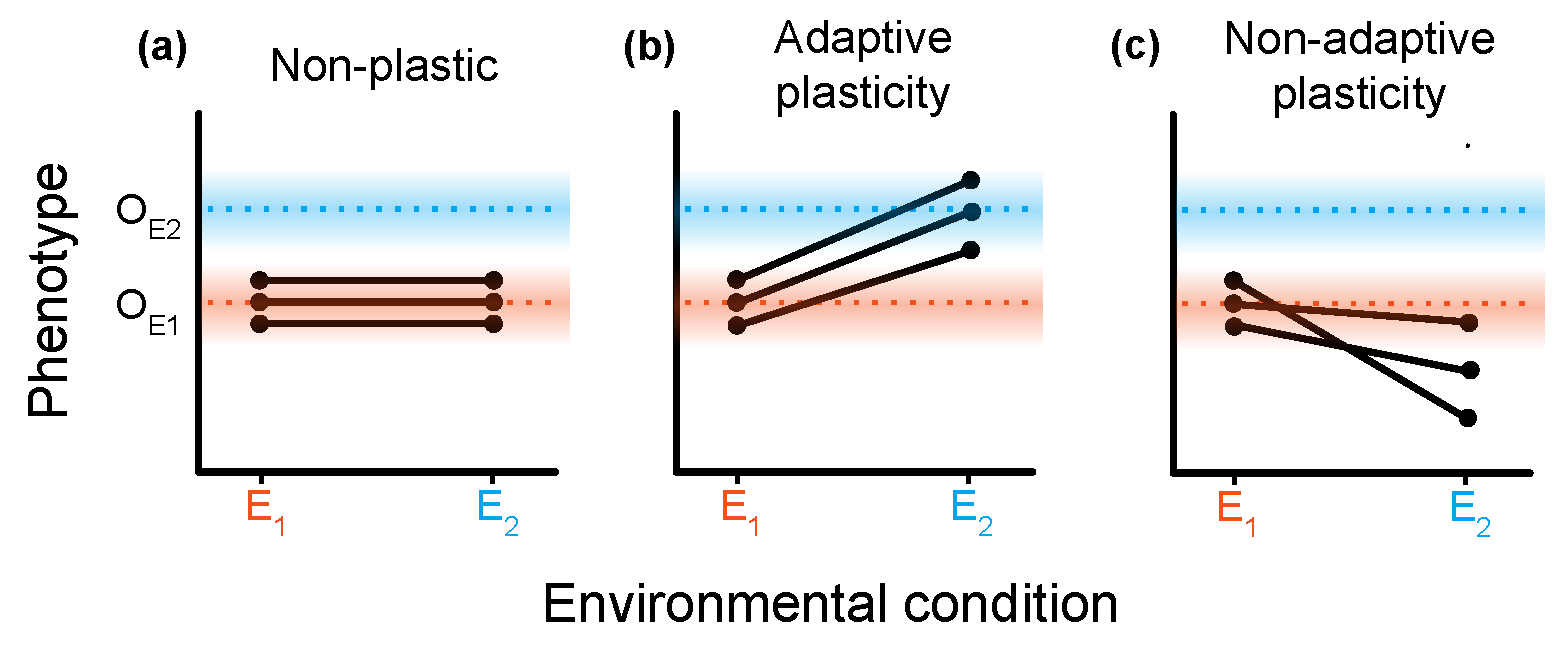
\includegraphics[width=0.85\textwidth]{05_consequences_of_plasticity/media/media-reaction-norms.pdf}
\caption{\small
\textbf{Hypothetical reaction norms for populations comprising genotypes placed in different environments.}
A reaction norm describes phenotypic change (or lack thereof) induced by environmental variation~\citep{west-eberhard_phenotypic_2008}. 
In all panels, two environmental conditions (denoted E$_1$ and E$_2$) are shown on the x-axis.
The y-axis indicates the phenotype expressed in each environment with O$_{\text{E}1}$ and O$_{\text{E}2}$ designating the optimal phenotype for E$_1$ and E$_2$, respectively.
Each pair of points connected by a solid black line denotes a genotype, with the points themselves representing its hypothetical phenotypes in each environment.
We present three scenarios for how populations could respond to a change from E$_1$ to E$_2$.
(a) A non-plastic population where phenotypes do not change with environmental shifts.  
% In such cases, we would expect strong directional selection toward O$_{\text{E}2}$ after the environment changes.
(b) An adaptively plastic population where phenotypes dynamically adjust to the new optimum. 
% As such, we would expect this population to remain relatively stable after the environment changes.
% (c) A population exhibiting non-adaptive plasticity with substantial variation in how individuals respond to the environmental change. In this case, we expect the change in environment to result in a rapid evolutionary sweep by genotypes closest to the new optimal phenotype.
% (d) A population exhibiting maladaptive plasticity. 
(c) A population exhibiting non-adaptive plasticity where environmental change induces phenotypes further away from the optimum. 
% relative to the given environmental change. 
% When the environment changes, there is little variation for selection to act on, and without beneficial mutations, this population could be at risk of extinction.
}
\label{fig:reaction-norms}
\end{figure}

% -- Plasticity as a source of cryptic variation --
Phenotypic plasticity allows for the accumulation of genetic variation in genomic regions that are unexpressed under current environmental conditions.
Such cryptic (``hidden'') genetic variation can serve as a source of diversity in the population, upon which selection can act when the environment changes \citep{schlichting_hidden_2008,levis_evaluating_2016}.
It remains unclear to what extent and under what circumstances this cryptic variation caches adaptive potential or merely accumulates deleterious alleles \citep{gibson_uncovering_2004,paaby_cryptic_2014,zheng_cryptic_2019}.

% -- Genes as followers --
The ``genes as followers'' hypothesis (also known as the ``plasticity first'' hypothesis) predicts that phenotypic plasticity may facilitate adaptive evolutionary change by producing variants with enhanced fitness under stressful or novel conditions \citep{west-eberhard_developmental_2003,schwander_genes_2011,levis_evaluating_2016}.
Environmentally-induced trait changes can be refined through selection over time (\textit{i.e.}, genetic accommodation).
Further, selection may drive plastic phenotypes to lose their environmental dependence over time in a process known as genetic assimilation \citep{west-eberhard_developmental_2005,pigliucci_phenotypic_2006,crispo_baldwin_2007,schlichting_phenotypic_2014,levis_evaluating_2016}.
In this way, environmentally-induced phenotypic changes can precede an evolutionary response.

% -- Plastic rescue + wrap up on plasticity background? --
Phenotypic plasticity may also ``rescue'' populations from extinction under changing environmental conditions by buffering populations against novel stressors.
This buffer promotes stability and persistence and grants populations time to further adapt to rapidly changing environmental conditions \citep{west-eberhard_developmental_2003,chevin_when_2010}.

Disparate predictions about how phenotypic plasticity may shift the course of subsequent evolution are not necessarily mutually exclusive.
Genetic and environmental contexts determine if, and to what extent, phenotypic plasticity promotes or constrains subsequent evolution.
Figure~\ref{fig:reaction-norms} overviews how we might expect different forms of phenotypic plasticity to result in different evolutionary responses after an environmental change.
In Figure~\ref{fig:reaction-norms}a, we would expect non-plastic populations to experience strong directional selection toward the new optimum (O$_{\text{E}2}$) after the environment changes.
We would expect an adaptively plastic population (Figure~\ref{fig:reaction-norms}b) to remain relatively stable after the environment changes, as plasticity shifts organisms' phenotypes to the new optimum.
In Figure~\ref{fig:reaction-norms}c, we would expect the non-adaptively plastic population to experience strong directional selection on their response to the new environmental conditions; indeed, such maladaptive plasticity may even put the population at risk of extinction in the absence of beneficial mutations.

%%%%%%%%%%%%%%%%%%%%%%
% -- Digital evolution --
%%%%%%%%%%%%%%%%%%%%%%
Experimental studies investigating the relationship between phenotypic plasticity and evolutionary outcomes can be challenging to conduct in natural systems.
Such experiments would require the ability to irreversibly toggle plasticity followed by long periods of evolution during which detailed phenotypic data would need to be collected.
Digital evolution experiments have emerged as a powerful research framework from which evolution can be studied.
In digital evolution, self-replicating computer programs (digital organisms) compete for resources, mutate, and evolve following Darwinian dynamics  \citep{wilke_biology_2002}.
Digital evolution studies balance the speed and transparency of mathematical and computational simulations with the open-ended realism of laboratory experiments.
Modern computers allow us to observe many generations of digital evolution at tractable time scales; thousands of generations can take mere minutes as opposed to months, years, or millennia.
Digital evolution systems also allow for perfect, non-invasive data tracking.
Such transparency permits the tracking of complete evolutionary histories within an experiment, which circumvents the historical problem of drawing evolutionary inferences using incomplete records (from frozen samples or fossils) and extant genetic sequences.
Additionally, digital evolution systems allow for experimental manipulations and analyses that go beyond what is possible in wet-lab experiments.
Such analyses have included exhaustive knockouts of every site in a genome to identify the functionality of each \citep{lenski_evolutionary_2003},
comprehensive characterization of local mutational landscapes \citep{lenski_genome_1999,canino-koning_fluctuating_2019},
and the real-time reversion of all deleterious mutations as they occur to isolate their long-term effects on evolutionary outcomes \citep{covert_experiments_2013}.
Furthermore, digital evolution studies allow us to directly toggle the possibility for adaptive plastic responses to evolve, which enables us to empirically test hypotheses that were previously relegated to theoretical analyses.

%%%%%%%%%%%%%%%%%%%%%%
% -- Overview of what we're testing / doing --
%%%%%%%%%%%%%%%%%%%%%%

In this study, we conduct digital evolution experiments to investigate how the evolution of adaptive phenotypic plasticity shifts the course of evolution in a cyclically changing environment.
We use the Avida Digital Evolution Platform \citep{ofria_avida:_2009}.
Avida is an open-source system that has been used to conduct a wide range of well-regarded studies on evolutionary dynamics, including
the origins of complex features \citep{lenski_evolutionary_2003},
the survival of the flattest effect \citep{wilke_evolution_2001},
and the origins of reproductive division of labor \citep{goldsby_evolutionary_2014}.
Our experiments build directly on previous studies in Avida that characterized the \textit{de novo} evolution of adaptive phenotypic plasticity \citep{clune_investigating_2007,lalejini_evolutionary_2016} as well as previous work investigating the evolutionary consequences of fluctuating environments for populations of non-plastic digital organisms \citep{li_digital_2004,canino-koning_fluctuating_2019}.
Of particular relevance, \cite{clune_investigating_2007} and \cite{lalejini_evolutionary_2016} experimentally demonstrated that adaptive phenotypic plasticity can evolve given the following four conditions (as described by \citealt{ghalambor_behavior_2010}):
(1) populations experience temporal environmental variation,
(2) these environments are differentiable by reliable cues,
(3) each environment favors different phenotypic traits,
and (4) no single phenotype exhibits high fitness across all environments.
We build on this previous work, but we shift our focus from the evolutionary causes of adaptive phenotypic plasticity to investigate its evolutionary consequences in a fluctuating environment.
Specifically, we examine the effects of adaptive plasticity on subsequent genomic and phenotypic change, the capacity to evolve and then maintain novel traits, and the accumulation of deleterious alleles.

% - what we did -
Each of our experiments are divided into two phases: in phase one, we precondition sets of founder organisms with differing plastic or non-plastic adaptations;
in phase two, we examine the subsequent evolution of populations founded with organisms from phase one under specific environmental conditions (Figure \ref{fig:experimental-design}).
First, we examine the evolutionary histories of phase two populations to test whether adaptive plasticity constrained subsequent genomic and phenotypic changes.
Next, we evaluate how adaptive plasticity influences how well populations produced by each type of founder can evolve and retain novel adaptive traits.
Finally, we examine lineages to determine whether adaptive plasticity facilitated the accumulation of cryptic genetic variation that would prove deleterious when the environment changed.

%%%%%%%%%%%%%%%%%%%%%%
% - Overview of findings -
%%%%%%%%%%%%%%%%%%%%%%
We found that the evolution of adaptive plasticity reduced subsequent rates of evolutionary change in a cyclic environment.
The non-plastic populations underwent more frequent selective sweeps and accumulated many more genetic changes over time, as non-plastic populations relied on genetic variation from \textit{de novo} mutations to continuously readapt to environmental changes.
The evolution of adaptive phenotypic plasticity buffered populations against environmental fluctuations, whereas repeated selective sweeps in non-plastic populations drove the accumulation of deleterious mutations and the loss of secondary beneficial traits. % via deleterious hitchhiking.
As such, adaptively plastic populations were better able to retain novel traits than their non-plastic counterparts.
In general, the evolution of adaptive phenotypic plasticity shifted evolutionary dynamics to be more similar to that of populations evolving in a static environment than to non-plastic populations evolving in an identical fluctuating environment.

\section{Materials and Methods}
\label{sec:methods}

\subsection{The Avida Digital Evolution Platform}
\label{sec:methods:avida}

% -- Define digital organisms --
Avida is a study system wherein self-replicating computer programs (digital organisms) compete for space on a finite toroidal grid \citep{ofria_avida:_2009}.
Each digital organism is defined by a linear sequence of program instructions (its genome) and a set of virtual hardware components used to interpret and express those instructions.
Genomes are expressed sequentially except when the execution of one instruction (\textit{e.g.}, a ``jump'' instruction) deterministically changes which instruction should be executed next.
Genomes are built using an instruction set that is both robust (\textit{i.e.}, any ordering of instructions is syntactically valid, though not necessarily meaningful) and Turing Complete (\textit{i.e.}, able to represent any computable function, though not necessarily in an efficient manner).
The instruction set includes operations for basic computations, flow control (\textit{e.g.}, conditional logic and looping), input, output, and self-replication.
% The virtual hardware set includes components such as a central processing unit (CPU) for executing instructions, registers to store values, buffers for inputs and outputs, and memory stacks \citep{ofria_avida:_2009}.

% -- Define reproduction & mutation --
Organisms in Avida reproduce asexually by copying their genome instruction-by-instruction and then dividing.
However, copy operations are imperfect and can result in single-instruction substitution mutations in an offspring's genome.
For this work, we configured copy operations to err at a rate of one expected mutation for every 400 instructions copied (\textit{i.e.}, a per-instruction error rate of 0.0025).
We held individual genomes at a fixed length of 100 instructions (the default genome size in Avida); that is, we did not include insertion and deletion mutations.
We used fixed-length genomes to control for treatment-specific conditions resulting in the evolution of substantially different genome sizes \citep{supplemental_material}\footnote{
We repeated our experiments without genome size restrictions and observed qualitatively similar results (see supplemental material, \citealt{supplemental_material}).
}, which could, on its own, drive differences in evolutionary outcomes among experimental treatments.
When an organism divides in Avida, its offspring is placed in a random location on the toroidal grid, replacing any previous occupant.
For this work, we used the default 60 by 60 grid size, which limits the maximum population size to 3600 organisms.
As such, improvements to the speed of self-replication are advantageous in the competition for space.

% -- Define fitness/metabolic rate/improving replication speed --
During evolution, organism replication rates improve in two ways: by improving genome efficiency (\textit{e.g.}, using a more compact encoding) or by accelerating the rate at which the genome is expressed (their ``metabolic rate'').
An organism's metabolic rate determines the speed at which it executes instructions in its genome.
Initially, an organism's metabolic rate is proportional to the length of its genome, but that rate is adjusted as it completes designated functions, such as performing Boolean logic functions \citep{ofria_avida:_2009}.
In this way, we can reward or punish particular phenotypic traits (\textit{i.e.}, Boolean logic functions).

\subsubsection{Phenotypic plasticity in Avida}
\label{sec:methods:avida:plasticity}

% -- Phenotypes & Phenotypic plasticity --
%   - What is a phenotype in Avida?
In this work, we measure a digital organism's phenotype as the set of Boolean logic functions that it performs (\textit{i.e.} expresses) in a given environment.
Sensory instructions in the Avida instruction set allow organisms to detect how performing a particular function would affect their metabolic rate (see supplemental material for more details, \citealt{supplemental_material}).
We define a phenotypically plastic organism as one that uses sensory information to alter which functions it performs based on the environment.

% -- Adaptive plasticity & non-adaptive plasticity --
Phenotypic plasticity in Avida can be adaptive or non-adaptive for a given set of environments.
Adaptive plasticity shifts net function expression closer to the optimum for the given environments.
Non-adaptive plasticity changes function expression in either a neutral or deleterious way.
In this work, optimal plasticity toggles functions to always perfectly match the set of rewarded functions for the given set of environments.

\subsection{Experimental design}
\label{sec:methods:experiment}

\begin{figure}[h!]
  \centering
  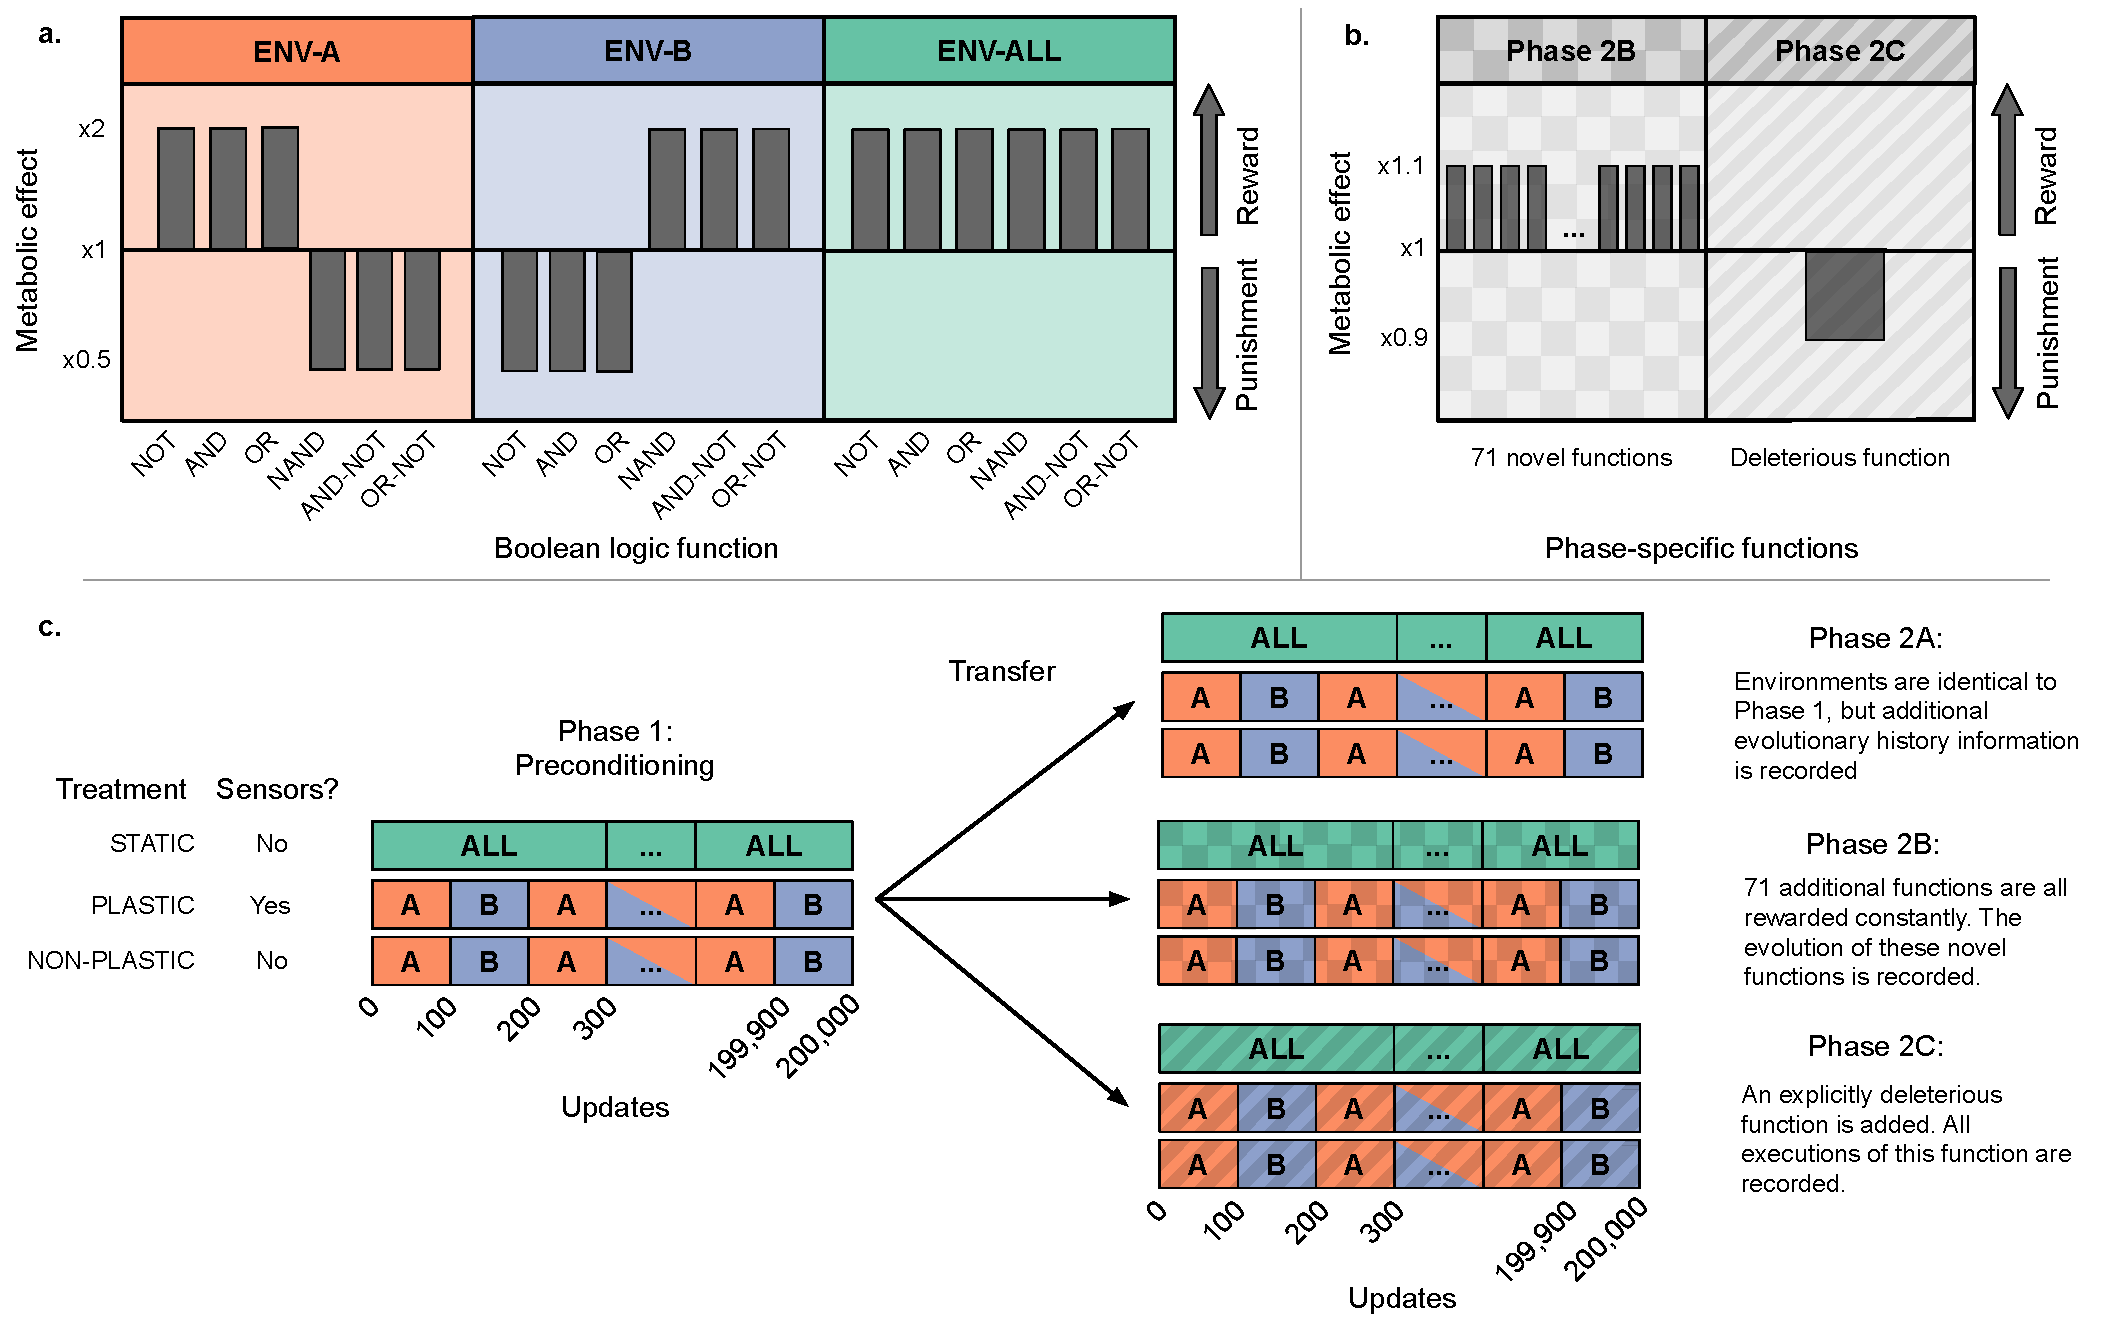
\includegraphics[width=1\textwidth]{05_consequences_of_plasticity/media/media-experimental-design.pdf}
  \caption{\small
  \textbf{Overview of experimental design.}
  The three plots in panel (a) show the environmental conditions used in every experiment and whether they reward or punish each base function.
  The two plots in (b) show the additional functions added in phases 2B and 2C. %Optional: phase 2A is not shown as it adds no additional functions
  %All novel tasks in phase 2B confer a 10\% metabolic reward, while executing the poisonous task in phase 2C causes a 10\% metabolic punishment (bars not drawn to scale).
  Panel (c) shows treatment differences and experimental phases.
  Treatments are listed on the left, with each treatment specifying its environmental configuration and whether sensors are functional.
  We conducted three independent two-phase experiments, each described on the right.
  Phases 2B and 2C are textured to match their function definitions in panel (b).
  Phase one is repeated for \textit{each} experiment with 100 replicate populations per treatment per experiment.
  For each replicate at the end of phase one, we used an organism of the most abundant genotype to found the second phase population.
  All STATIC and NON-PLASTIC populations move on to phase two, but PLASTIC populations only continue to the second phase if their most abundant genotype exhibits optimal plasticity.
  Metrics are recorded only in phase two.
  }
  \label{fig:experimental-design}
\end{figure}

%%%%%%%%%%%%%%%%%%%%%%%%%%%%%%%%%%%%%%%%%%%%%%%%%
% OUTLINE
%%%%%%%%%%%%%%%%%%%%%%%%%%%%%%%%%%%%%%%%%%%%%%%%%
% Overview of experimental design - with diagram (not a subsubsection?)
% - Focused around diagram
% Environment implementations
% Specifications for Phase 1
% specifications for Phase 2A
% specifications for Phase 2B
% specifications for Phase 2C
%%%%%%%%%%%%%%%%%%%%%%%%%%%%%%%%%%%%%%%%%%%%%%%%%

% -- Treatments --
We conducted three independent experiments using Avida to investigate how the evolution of adaptive plasticity influences evolutionary outcomes in fluctuating environments.
For each experiment, we compared the evolutionary outcomes of populations evolved under three treatments (Figure \ref{fig:experimental-design}):
(1) a \textbf{PLASTIC} treatment where the environment fluctuates, and digital organisms can use sensory instructions to differentiate between environmental states;
(2) a \textbf{NON-PLASTIC} treatment with identical environment fluctuations, but where sensory instructions are disabled;
and (3) a \textbf{STATIC} control where organisms evolve in a constant environment.

% -- Experiment phases --
Each experiment was divided into two phases that each lasted for 200,000 updates\footnote{
    One update in Avida is the amount of time required for the average organism to execute 30 instructions.
    See \citep{ofria_avida:_2009} for more details.
} of evolution (Figure~\ref{fig:experimental-design}), which is equivalent to approximately 30,000 to 40,000 generations.
% Phase one of each experiment was an acclimation phase.
In phase one of each experiment, we evolved plastic, non-plastic, and control organisms for use in phase two.
In phase two, we founded new populations with these evolved organisms and examined their subsequent evolution under given combinations of treatment and experimental conditions.
During phase two, we tracked and saved each population's evolutionary history as well as saving the full final population.
Phase one was for preconditioning only; all comparisons between treatments were performed on phase two data.

\subsubsection{Environments}
\label{sec:methods:experiment:environments}

% ----- ENVIRONMENTS -----
% traits_set_a <- c("not", "and", "or")
% traits_set_b <- c("nand", "ornot", "andnot")

% -- Environment definitions --
% In all of our experiments, populations evolve in either static or fluctuating environments.

We constructed three experimental environmental conditions, abbreviated hereafter as ``ENV-A'', ``ENV-B'', and ``ENV-ALL''.
In ENV-A, organisms are rewarded for expressing the NOT, AND, and OR Boolean logic functions, and organisms are punished for expressing the NAND, AND-NOT, and OR-NOT functions. 
ENV-B is the reverse of ENV-A; that is, in ENV-B, organisms are rewarded for expressing the NAND, AND-NOT, and OR-NOT functions and are punished for expressing the NOT, AND, and OR functions.
In ENV-ALL, organisms are rewarded for expressing each of the NOT, AND, OR, NAND, AND-NOT, and OR-NOT functions.
In all environmental conditions (ENV-A, ENV-B, and ENV-ALL), a rewarded function expressed by an organism doubles their metabolic rate, allowing them to execute twice as many instructions in the same amount of time.
A punished function halves an organism's metabolic rate.
Each Boolean logic function is a non-trivial trait to evolve, as they each require the coordination of multiple genetic instructions to express~\citep{lenski_evolutionary_2003}.

% Figure \ref{fig:experimental-design} describes these environments based on whether each of six Boolean logic tasks (NOT, NAND, AND, OR-NOT, OR, and AND-NOT) is rewarded or punished.

% -- Treatment-specific environment details --
In both the PLASTIC and NON-PLASTIC treatments, the environment cycles between equal-length periods of ENV-A and ENV-B.
Each of these periods persist for 100 updates (approximately 15 to 20 generations).
Thus, populations experience a total of 1,000 full periods of ENV-A interlaced with 1,000 full periods of ENV-B during each experimental phase.
Previous work has shown that this rate of change reliably allows for thot Alternative for Visual Comparison of Distributions. These provide a side-by-side display that contains the density curve, the origie evolution of adaptive phenotypic plasticity in Avida~\citep{clune_investigating_2007,lalejini_evolutionary_2016}.

% -- Sensory instructions + control flow and controlling the capacity for plasticity --
Organisms in the PLASTIC treatments differentiate between ENV-A and ENV-B by executing one of six sensory instructions, each associated with a particular Boolean logic function; these sensory instructions detect whether their associated function is currently rewarded or punished.
By using sensory information in combination with execution flow-control instructions, organisms can conditionally perform different functions depending on the current environmental conditions.

\subsubsection{Experiment Phase 1 -- Environment preconditioning}
\label{sec:methods:experiment:phase-one}

For each treatment, we founded 100 independent populations from a common ancestral strain capable only of self-replication.
At the end of phase one, we identified the most abundant (\textit{i.e.}, dominant) genotype and sampled an organism with that genotype from each replicate population to found a new population for phase two.

For the PLASTIC treatment, we needed to ensure that our observations during the second phase of each experiment reflected the evolutionary consequences of adaptive plasticity. 
To do so, measured the plasticity of each PLASTIC-treatment population's dominant genotype by independently testing that genotype in each of ENV-A and ENV-B and recording the phenotype expressed in each environment.
We discarded PLASTIC-treatment phase one populations if the dominant genotype did not exhibit optimal plasticity (as defined in Section~\ref{sec:methods:avida:plasticity}), which ensured that PLASTIC-treatment phase two populations were founded with an optimally plastic organism.

% For the PLASTIC treatment, we measure the plasticity of each population's dominant genotype by independently testing the given genotype in each of ENV-A and ENV-B and recording the phenotype expressed in each environment.
% We discard PLASTIC-treatment phase one populations if the dominant genotype does not exhibit optimal plasticity (as defined in Section \ref{sec:methods:avida:plasticity}).
% This approach ensures that measurements taken on PLASTIC-treatment populations during the second phase of each experiment reflect the evolutionary consequences of adaptive plasticity.

\subsubsection{Experiment Phase 2A -- Evolutionary change rate}
\label{sec:methods:exp:evolutionary-change-rate}

We conducted experiment phase 2A to test for differences in evolutionary change---the accumulation of genetic and phenotypic changes---among populations evolving under each of our three treatment conditions (PLASTIC, NON-PLASTIC, and STATIC). 
Phase 2A continued exactly as phase one, except we tracked the rates of evolutionary change in each of the PLASTIC-, NON-PLASTIC-, and STATIC-treatment populations.
Specifically, we quantified evolutionary change using four metrics (each described in Table~\ref{tab:metrics-definitions}):
(1) coalescence event count,
(2) mutation count,
(3) phenotypic volatility,
and (4) mutational robustness.

While environmental conditions during phases one and 2A are identical, these phases are distinct in how populations are founded: each phase one population is founded with a common ancestor capable only of self-replication, whereas each phase two population is founded with an organism that was evolved in its treatment-specific conditions.
Thus, during phase two, phylogenies are rooted with an ancestor that is well-adapted to its treatment conditions, which, in turn, ensures that our observations can exclude dynamics associated with initial adaptation.

\subsubsection{Experiment Phase 2B -- Novel function evolution}
\label{sec:methods:exp:novel-task-evolution}

We conducted experiment phase 2B to quantify the extent to which organisms evolved under PLASTIC-, NON-PLASTIC-, and STATIC-treatment conditions were able to acquire and retain novel functions. 
Phase 2B extended the conditions of phase one by adding 71 novel Boolean logic functions~\citep{ofria_avida:_2009}, which were always rewarded in all treatments.
The original six phase one functions (NOT, NAND, AND, OR-NOT, OR, and AND-NOT; hereafter called ``base'' functions) continued to be rewarded or punished according to the particular treatment conditions.
% @CAO: line below can be restored (and reworded) if readers need help with the intuition.
%As such, in fluctuating environments, the six base tasks continued to fluctuate, but the additional 71 tasks were always rewarded; in static environments, performing any of the 77 logic tasks was always beneficial.
An organism's metabolic rate was increased by \novelTraitsReward\ for each novel function that it expressed (limited to one reward per function).
This reward provided a selective pressure to evolve these functions, but their benefits did not overwhelm the 100\% metabolic rate increase conferred by rewarded base functions.
As such, populations in the PLASTIC and NON-PLASTIC treatments could not easily escape environmental fluctuations by abandoning the fluctuating base functions.

During this experiment, we used three metrics to quantify novel function acquisition and retention in evolving populations (each described in Table~\ref{tab:metrics-definitions}):
% During this experiment, we tracked the extent to which populations evolving under each treatment were capable of acquiring and retaining novel tasks.
% Specifically, we used three metrics (each described in Table~\ref{tab:metrics-definitions}):
(1) final novel function count,
(2) novel function discovery,
and (3) novel function loss.

\subsubsection{Experiment Phase 2C -- Deleterious instruction accumulation}
\label{sec:methods:exp:deleterious-instruction-accumulation}

We conducted experiment phase 2C to quantify the extent to which organisms evolved under PLASTIC-, NON-PLASTIC-, and STATIC-treatment conditions acquired deleterious instructions via mutation.
Phase 2C extended the instruction set of phase one with a \code{deleterious} instruction.
When an organism executes a \code{deleterious} instruction, it performs a ``deleterious'' function, which reduces the organism's metabolic rate (and thus reproductive success) but does not otherwise alter the organism's behavior.
We imposed a 10\% penalty each time an organism performed the deleterious function, making the \code{deleterious} instruction explicitly harmful to execute.
We did not limit the number of times that an organism could perform the deleterious function, and as such, organisms could perform the deleterious function as many times as they executed the \code{deleterious} instruction.

We tracked the number of times each organism along the dominant lineage performed the deleterious function.
Specifically, we used two metrics (each described in Table~\ref{tab:metrics-definitions}):
(1) final deleterious function count and (2) deleterious function acquisition count.

\subsection{Experimental analyses}

%\newcommand*{\theadalt}[1]{\multicolumn{1}{c}{\bfseries #1}}

\setlength{\tabcolsep}{16pt}
\renewcommand{\arraystretch}{1.5}
\begin{table}[ht]
    \centering

    %\rowcolors{2}{gray!25}{white}
    \begin{tabularx}{\linewidth}{lX} % p{10cm}
        \rowcolor{gray!50}
        \hline
        \theadalt{Metric} & \theadalt{Description}   \\
        \hline
        \rowcolor{gray!25}
        \SweepsMetricName & \SweepsMetricDesc \\
        \rowcolor{white}
        \MutationCountMetricName & \MutationCountMetricDesc \\
        \rowcolor{gray!25}
        \PhenotypicVolatilityMetricName & \PhenotypicVolatilityMetricDesc \\
        \rowcolor{white}
        \MutationalStabilityMetricName & \MutationalStabilityMetricDesc \\
        \rowcolor{gray!25}
        \TaskPerformanceMetricName & \TaskPerformanceMetricDesc \\
        \rowcolor{white}
        \TaskDiscoveryMetricName & \TaskDiscoveryMetricDesc \\
        \rowcolor{gray!25}
        \TaskLossMetricName & \TaskLossMetricDesc \\
        \rowcolor{white}
        \FinalPoisonMetricName & \FinalPoisonMetricDesc \\
        \rowcolor{gray!25}
        \LineagePoisonMetricName & \LineagePoisonMetricDesc \\
        \hline
    \end{tabularx}

    \caption{\textbf{Metric descriptions.}}
    \label{tab:metrics-definitions}
\end{table}


% naive environment = what organism experiencing
% alternative environment = what organism is not currently experiencing

% - How we extracted representative lineages -
For each of our experiments, we tracked and analyzed the phylogenetic histories of evolving populations during phase two and generated a set of summary statistics (Table~\ref{tab:metrics-definitions}).
For each phylogenetic history, we counted the number of times that the most recent common ancestor for the population shifted and used this value as the number of coalescence events.
Next, at the final time point, we identified the most abundant genotype in the evolved population, and chose a \textit{representative organism} from that genotype for further analysis.
% We then isolated the lineage from the founding organism to the representative organism, which we used as the representative lineage for further analysis.
% We used the lineage from the founding organism to the representative organism as the \textit{representative lineage} for further analysis.
We used the lineage from the founding organism to the representative organism to summarize the evolutionary pathway of a population. 
This lineage represents the majority of the evolutionary history from the given population as long as the entire population traces back to the lineage in recent history.
We manually inspected evolved phylogenies and found no evidence that any of our experimental treatments supported long-term coexistence.
As such, analyses of the representative lineages reflect the majority of evolutionary history for a given population.

% To be confident that each representative lineage reflected the majority of the evolutionary history from a given populuation at the end of the ex
% [These lineages represent the majority of the evolutionary history from a given population only if there aren't members of the population that haven't diverged too far in the past / only if single the entire population traces back to that lineage in recent history (i.e., no long-term coexistence)].
% We manually inspected evolved phylogenies and found no evidence that any of our experimental treatments supported long-term coexistence.
% As such, each of the representative lineages reflect the majority of evolutionary history from a given population at the end of our experiment.

% -- PHENOTYPIC PROFILE --
% DEFINE PHENOTYPIC PROFILE - metric definitions will use this.
Some of our metrics (Table \ref{tab:metrics-definitions}) required us to measure genotype-by-environment interactions.
Importantly, in the fluctuating environments, we needed to differentiate phenotypic changes that were caused by mutations from those that were caused by environmental changes.
To accomplish this, we produced organisms with the given focal genotype, measured their phenotype in each environmental condition, and aggregated the resulting phenotypes to create a \textit{phenotypic profile}.
Although organisms with different genotypes may express the same set of functions across environmental conditions, their phenotypic profiles may not necessarily be the same.
For example, an organism that expresses NOT in ENV-A and NAND in ENV-B has a distinct phenotypic profile from one that expresses NAND in ENV-A and NOT in ENV-B.
Because phenotypic profiles encapsulate function expression across all relevant environmental conditions (ENV-A and ENV-B), a change in phenotypic profile from parent to offspring indicates a mutationally-induced phenotypic change.  

% -- GENETIC MANIPULATION / MUTATIONAL NEIGHBORHOOD --
% How do we produce mutants for analyses?
While most analyses employed here are retrospective metrics applied to lineages, digital evolution allows precise manipulations on individual organisms and genomes.
Mutational robustness uses this technique when looking at the possible mutations on a representative genotype.
Genomes in Avida are linear sequences of instructions, and as such, possible mutations can be simulated by substituting other instructions at the desired site.
Indeed, the mutational robustness of a genotype examines all one-step mutations (\textit{i.e.}, each mutation where exactly one instruction is substituted).
This allows us to disentangle whether the frequency of mutationally-induced phenotypic changes observed along a lineage is a consequence of evolved genetic architectures versus the result of population dynamics that actively skewed the distribution of organisms along the lineage; that is, are genomes organized such that mutations are more likely to induce phenotypic changes, or are organisms with phenotypes different from their parents more likely to be successful and thus appear along the representative lineage?

% the results of the lineage metrics are a consequence of evolved genetic architectures versus ongoing population dynamics that are actively skewing the distribution of organisms along each lineage. %or the results of selection.
%otherwise.
%purely the results of selection.


\subsection{Statistical analyses}

Across all of our experiments, we differentiated between sample distributions using non-parametric statistical tests.
For each major analysis, we first performed a Kruskal-Wallis test \citep{kruskal_use_1952} to
determine if there were significant differences in results from the PLASTIC, NON-PLASTIC, and STATIC treatments (significance level $\alpha=0.05$).
If so, we applied a Wilcoxon rank-sum test \citep{kotz_individual_1992} to distinguish between pairs of treatments.
We applied Bonferroni corrections for multiple comparisons \citep{rice_analyzing_1989} where appropriate.

\subsection{Software availability}

We conducted our experiments using a modified version of the Avida software, which is open source and freely available on \href{https://github.com/amlalejini/evolutionary-consequences-of-plasticity}{GitHub}~\citep{supplemental_material}.
Modifications to Avida included an improved phylogeny tracking system that enabled us to track coalescence events and the addition of custom sensory instructions specific to our experiments.
We used Python for data processing, and we conducted all statistical analyses using R version 4~\citep{r_core_team_r_v4}.
We used the tidyverse collection of R packages~\citep{r_tidyverse_2019} to wrangle data, and we used the following R packages for analysis, graphing, and visualization:
ggplot2~\citep{R-ggplot2},
cowplot~\citep{R-cowplot},
Color Brewer~\citep{harrower_colorbrewerorg_2003,R-Brewer_2014},
rstatix~\citep{R-rstatix},
ggsignif~\citep{R-ggsignif},
scales~\citep{R-scales},
Hmisc~\citep{R-Hmisc},
fmsb~\citep{R-fmsb},
and boot~\citep{R-boot}.
We used R markdown~\citep{rmarkdown} and bookdown~\citep{R-bookdown} to generate web-enabled supplemental material.
All of the source code for our experiments and analyses, including configuration files and guides for replication, can be found in our supplemental material, which is hosted on \href{https://github.com/amlalejini/evolutionary-consequences-of-plasticity}{GitHub}~\citep{supplemental_material}.
Additionally, our experimental data is available on the Open Science Framework at \url{https://osf.io/sav2c/} \citep{osf_data}.

%%%%%%%%%%%%%%%%%%%%%%%%%%%%%%%%%%%%%%%%%%%%%%%%%%%%%%%%%%%%
% INSTRUCTIONS:
% This section may be divided by subheadings. Footnotes should not be used and must be transferred to the main text.
%%%%%%%%%%%%%%%%%%%%%%%%%%%%%%%%%%%%%%%%%%%%%%%%%%%%%%%%%%%%

\section{Results}

\subsection{Adaptive phenotypic plasticity slows evolutionary change in fluctuating environments}

\begin{figure}[h!]
  \centering
  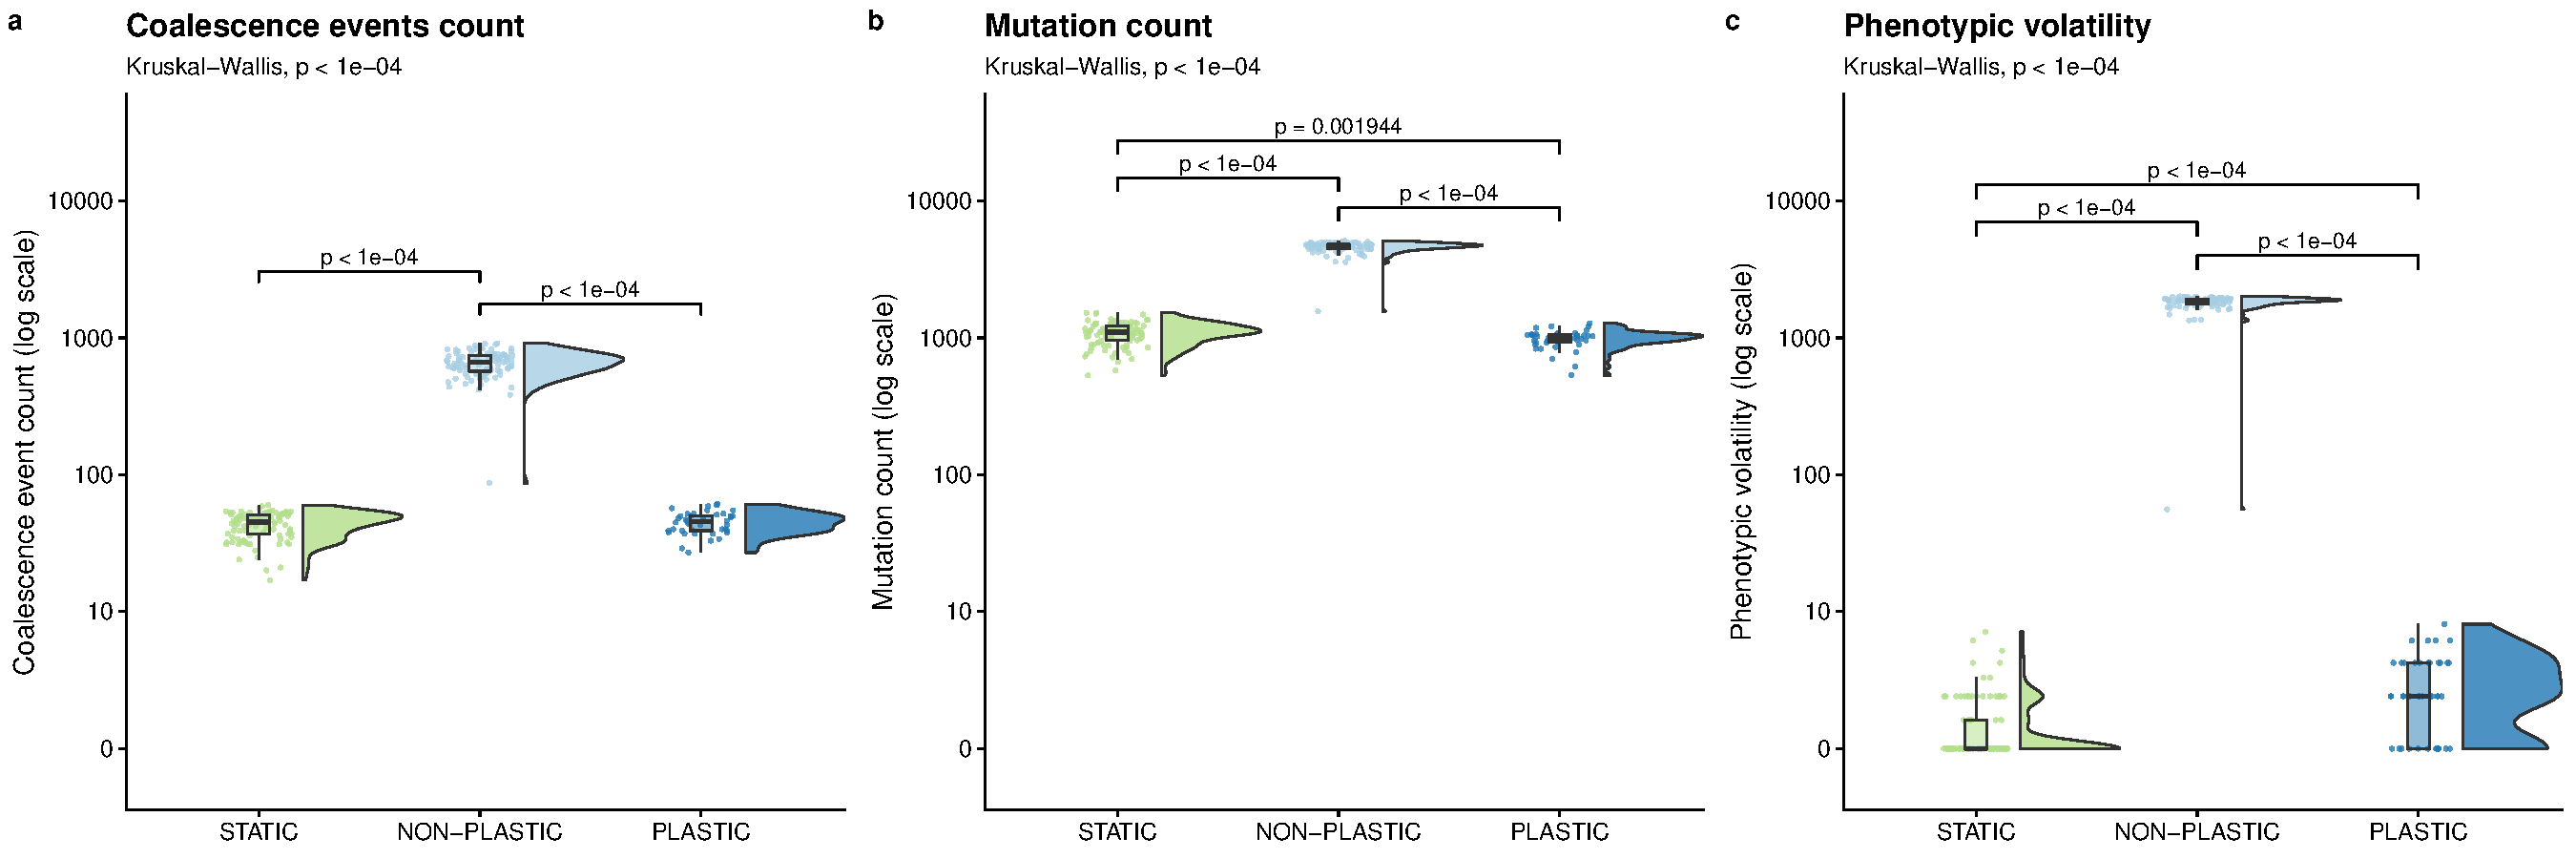
\includegraphics[width=1\textwidth]{05_consequences_of_plasticity/media/media-evolutionary-change-magnitude-panel.pdf}
  \caption{\small
  \textbf{Magnitude of evolutionary change.}
  Raincloud plots~\citep{allen_raincloud_2019} of
  (a) coalescence event count,
  (b) mutation count,
  and (c) phenotypic volatility.
  See Table~\ref{tab:metrics-definitions} for descriptions of each metric.
  Each plot is annotated with statistically significant comparisons (Bonferroni-corrected pairwise Wilcoxon rank-sum tests).
  Note that adaptive phenotypic plasticity evolved in \evolutionaryChangeRatePlasticReps\ of \evolutionaryChangeRateReplicates\ replicates from the PLASTIC treatment during phase one of this experiment; we used this more limited group to found \evolutionaryChangeRatePlasticReps\ phase-two PLASTIC replicates from which we report these PLASTIC data.
  }
  \label{fig:evolutionary-dynamics-magnitude}
\end{figure}


%%%%%%%%%%%%%%%%%%%%%%%%%%%%%%%%%
% Results to report (2021-02-08 experiment)
% ----- GENERATIONS -----
% - average generations elapsed (of a population)
%   - NON-PLASTIC (median: 41768.65) > PLASTIC (median: 31697.65) > STATIC (median: 30839.75)
%   condition     mean    sd
%   <chr>        <dbl> <dbl>
% 1 NON-PLASTIC 41090. 2702.
% 2 PLASTIC     31016. 2615.
% 3 STATIC      30002. 3011.

%
% ----- SWEEPS -----
% - coalescence events (total)
%   - NON-PLASTIC (median: 663.5) > ( PLASTIC (median: 45.5) ~~ STATIC (median: 45) )
% - Average number of generations between coalescence events (gens / sweeps)
%   - ( PLASTIC (median: 685.001780758557) ~~ STATIC (median: 693.676265008576) ) > NON-PLASTIC (median: 62.0184902295191)
%
% ----- PHENOTYPIC VOLATILITY -----
% - phenotypic volatility (total)
%   - i.e., total number of times phenotypes change along lineages
%   - NON-PLASTIC (median: 1868) > PLASTIC (median: 2) > STATIC (median: 0)
% - phenotypic volatility / lineage length
%   - i.e., how often do genomic changes reflect changes in phenotype?
%   - NON-PLASTIC (median: 0.437) > PLASTIC (median: 0.0022) > STATIC (median: 0)
% - phenotypic volatility / generations
%   - i.e., per-offspring rate of phenotypic changes
%   - NON-PLASTIC (median: 0.0447) > PLASTIC (median: 6.33e-05) > STATIC (median: 0)
%
% ----- MUTATION ACCUMULATION -----
% - mutation accumulation (total)
%   - NON-PLASTIC (median: 4657.5) > STATIC (median: 1100) > PLASTIC (median: 998.5)
% - mutation accumulation / lineage length
%   - NON-PLASTIC (median: 1.10048311715591) > STATIC (median: 1.03794597464116) > PLASTIC (median: 1.0328599144651)
% - mutation accumulation / generation
%   - NON-PLASTIC (median: 0.11) > STATIC (median: 0.0368) > PLASTIC (median: 0.0319)
%
% ----- MUTATIONAL EFFECTS -----
% - fraction of mutational steps that alter (aggregate) phenotype
%   - NON-PLASTIC (mean: 0.434007, CI [0.4242,  0.4406]) > PLASTIC (mean: 0.002717008, 0.0020,  0.0035) > STATIC (mean: 0.0006788834, CI [0.0004,  0.0009])
% - fraction of phenotype-altering mutation steps that alter unexpressed phenotype (PLASTIC condition only)
%   - mean: 0.8247126 CI [0.7443,  0.8994]
% - fraction of mutations that affect unexpressed phenotype that are deleterious (PLASTIC only)
%   - mean: 0.5172414 CI [0.4402,  0.5977]
% - fraction of mutations that affect unexpressed phenotype that are beneficial (PLASTIC only)
%   - mean: 0.4827586 CI [0.4046,  0.5598]
%%%%%%%%%%%%%%%%%%%%%%%%%%%%%%%%%

% -- Magnitude of evolutionary change --
%  - Selective sweeps
%  - Mutation accumulation
%  - Phenotypic volatility
In experimental phase 2A,
we tested whether adaptive phenotypic plasticity constrained or promoted subsequent evolutionary change in a fluctuating environment.
First, we compared the total amount of evolutionary change in populations evolved under the PLASTIC, NON-PLASTIC, and STATIC treatments as measured by coalescence event count, mutation count, and phenotypic volatility (Figure~\ref{fig:evolutionary-dynamics-magnitude}).
According to each of these metrics, NON-PLASTIC populations experienced a larger magnitude of evolutionary change than either PLASTIC or STATIC populations.
We observed significantly higher coalescence event counts in NON-PLASTIC populations than in PLASTIC or STATIC populations (Figure~\ref{fig:evolutionary-dynamics-magnitude}\hyperref[fig:evolutionary-dynamics-magnitude]{a}).
NON-PLASTIC lineages had significantly higher mutation counts (Figure~\ref{fig:evolutionary-dynamics-magnitude}b) and phenotypic volatility than PLASTIC or STATIC lineages (Figure~\ref{fig:evolutionary-dynamics-magnitude}c).

% -- Elapsed generations --
Changing environments have been shown to increase generational turnover (\textit{i.e.}, how rapidly generations elapse) in Avida populations~\citep{canino-koning_evolution_2016}, which could explain why we observe a larger magnitude of evolutionary change at the end of 200,000 updates of evolution in NON-PLASTIC populations.
Indeed, we found that significantly more generations of evolution elapsed in NON-PLASTIC populations (mean of $41090\pm2702$ std. dev.) than in PLASTIC (mean of $31016\pm2615$ std. dev.) or STATIC (mean of $30002\pm3011$ std. dev.) populations during phase 2A (corrected Wilcoxon rank-sum tests, p $<10^{-4}$).

% -- Rate of evolutionary change => intuition --
To evaluate whether increased generational turnover explains the greater magnitude of evolutionary change in NON-PLASTIC populations, we examined the average number of generations between coalescence events and the realized mutational robustness of lineages (Table \ref{tab:metrics-definitions}).
A coalescence event indicates a selective sweep, which is a hallmark of adaptive evolutionary change.
Realized mutational robustness measures the frequency that mutations cause phenotypic changes along a lineage.
We expect that static conditions should favor fit lineages with high realized mutational robustness that no longer undergo rapid adaptive change and hence do not trigger frequent coalescence events.
Under fluctuating conditions, however, lineages must be composed of plastic organisms if they are to maintain both high fitness and realized mutational robustness.
Without plasticity, we expect fluctuating conditions to produce lineages with low realized mutational robustness and frequent coalescence events as populations must continually acquire and fix mutations to readapt to the environment.

\begin{figure}[h!]
  \centering
  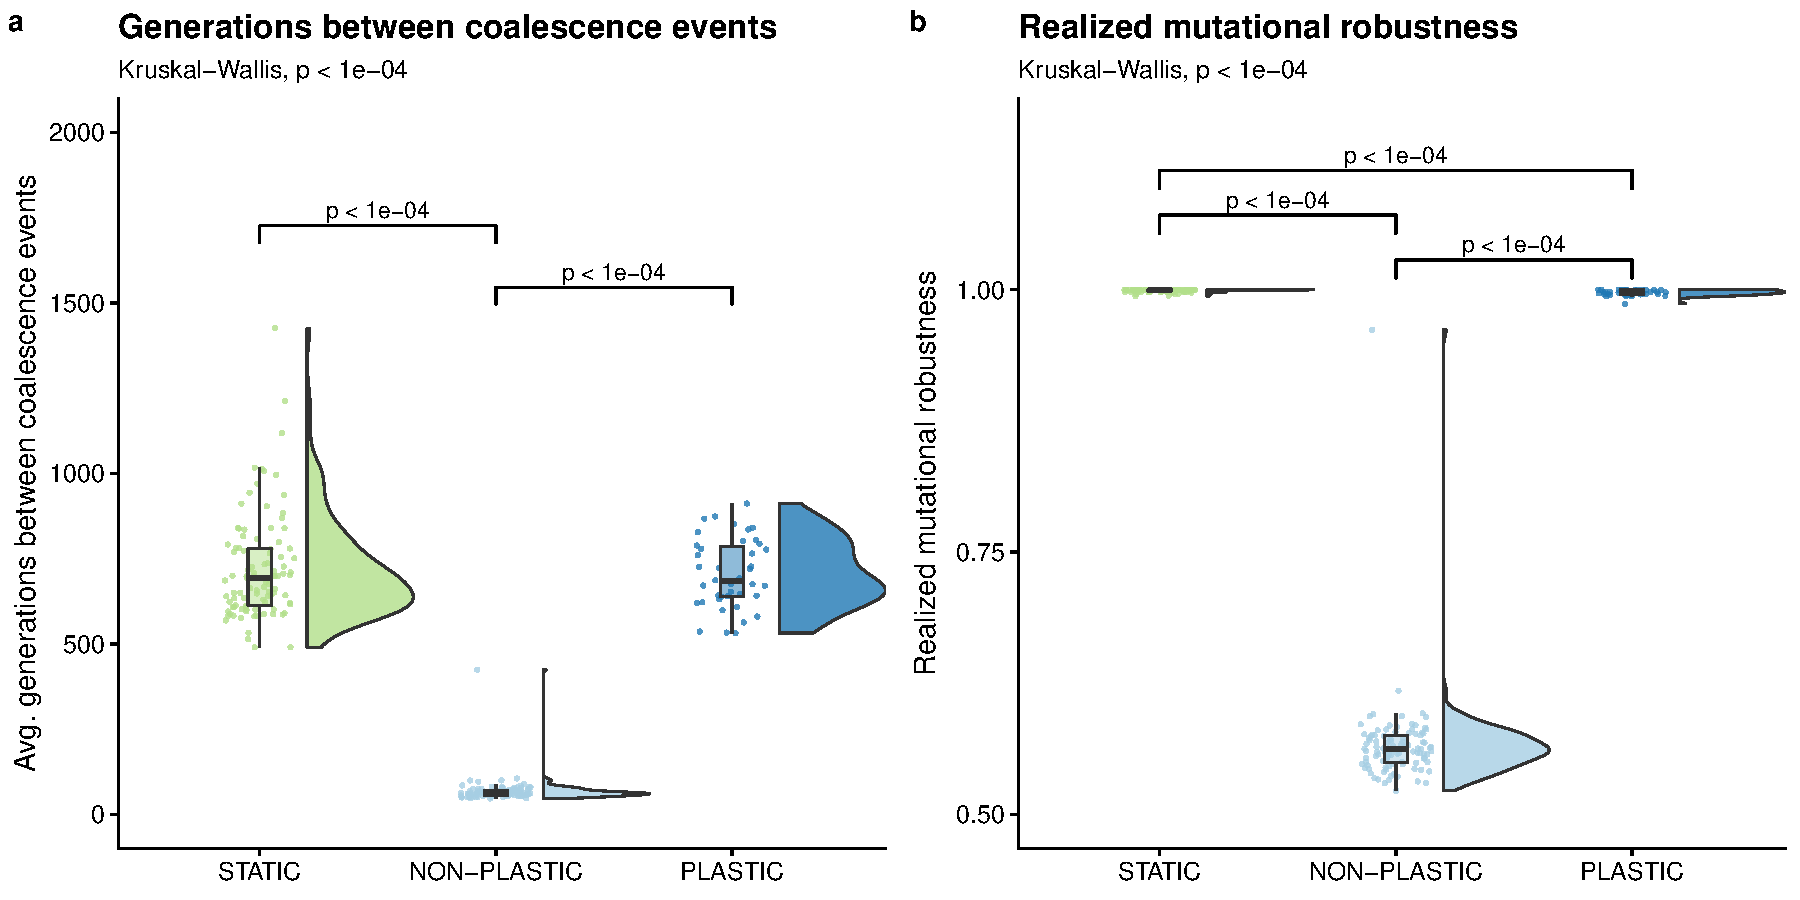
\includegraphics[width=0.66\textwidth]{05_consequences_of_plasticity/media/media-evolutionary-change-pace-panel.pdf}
  \caption{\small
  \textbf{Pace of evolutionary change.}
  Raincloud plots of
  (a) average number of generations between coalescence events,
  and (b) realized mutational robustness (Table \ref{tab:metrics-definitions}).
  Each plot is annotated with statistically significant comparisons (Bonferroni-corrected pairwise Wilcoxon rank-sum tests).
  }
  \label{fig:evolutionary-dynamics-rate}
\end{figure}

% -- Rate of evolutionary change => findings --
On average, significantly fewer generations elapsed between coalescence events in NON-PLASTIC populations than in either PLASTIC or STATIC populations (Figure \ref{fig:evolutionary-dynamics-rate}a).
We also found that both STATIC and PLASTIC lineages exhibited higher realized mutational robustness relative to that of NON-PLASTIC lineages (Figure \ref{fig:evolutionary-dynamics-rate}b); that is, mutations observed along NON-PLASTIC lineages more often caused phenotypic changes in offspring.
Overall, our results indicate that NON-PLASTIC populations underwent more rapid (and thus a greater amount of) evolutionary change than either PLASTIC or STATIC populations.

% -- Mutational stability in static and plastic lineages --
While both STATIC and PLASTIC lineages exhibited high realized mutational robustness, we found that STATIC lineages exhibited higher realized robustness than PLASTIC lineages (Figure \ref{fig:evolutionary-dynamics-rate}b).
Overall, there were rare instances of mutations that caused a change in phenotypic profile across all PLASTIC lineages.
Of these mutations, we found that over 80\% (83 out of 102) of changes to phenotypic profiles were cryptic.
That is, the mutations affected traits that would not have been expressed in the environment that the organism was born into but would have been expressed had the environment changed.

\begin{figure}[ht!]
  \centering
  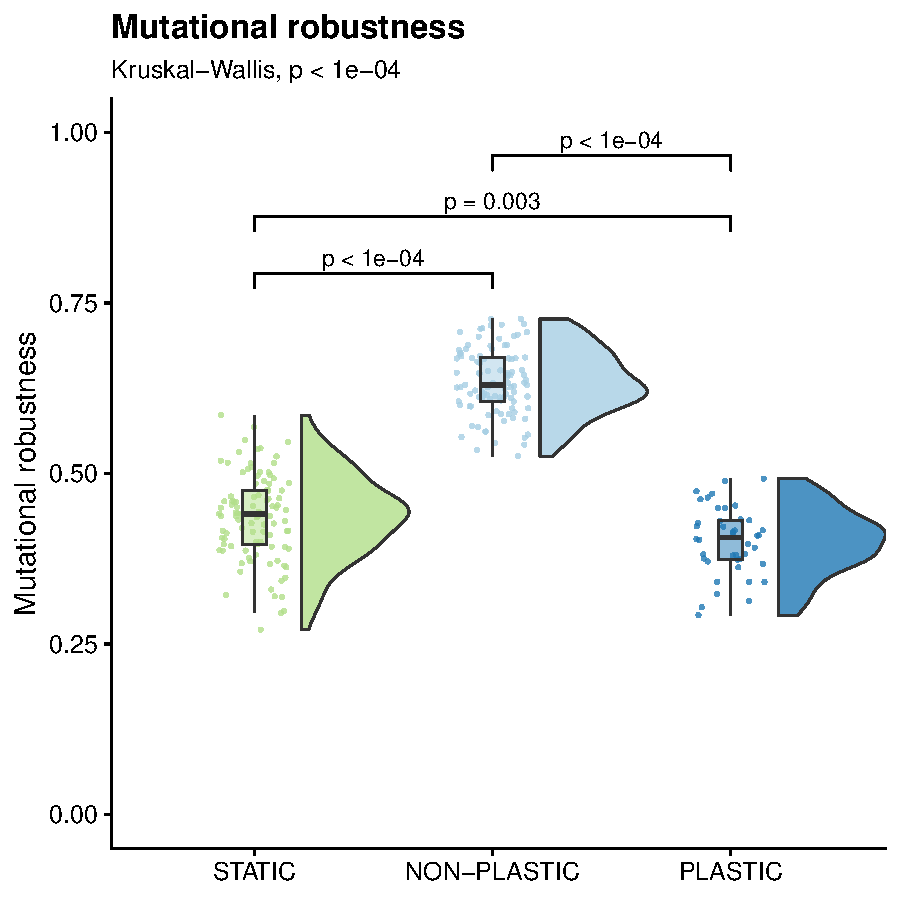
\includegraphics[width=0.33\textwidth]{05_consequences_of_plasticity/media/media-mutational-robustness.pdf}
  \caption{\small
      \textbf{Mutational robustness.}
      Raincloud plot of mutational robustness of each representative genotype (Table \ref{tab:metrics-definitions}).
      The plot is annotated with statistically significant comparisons (Bonferroni-corrected pairwise Wilcoxon rank-sum tests).
  }
  \label{fig:mutational-robustness}
\end{figure}

% -- mutational landscaping --
% Thus far, our analyses have focused on dominant lineage.
% What about mutations off the line of descent?
% Mutational stability result is NOT due to random mutations being more likely to induce phenotypic change.
% KEY: Motivation for looking at mutational neighborhoods needs to made very clear here
%   - Why not look at mutational neighborhoods for the other experiments?
Given that NON-PLASTIC lineages exhibited the lowest realized mutational robustness of our three experimental treatments, we sought to determine if this effect was driven by differences in evolved genetic architectures.
Specifically, did the NON-PLASTIC genetic architectures evolve such that mutations were more likely to result in phenotypic change?
Such a mutational bias would trade off descendant fitness in the same environment in exchange for a chance of increasing descendant fitness in alternate environments.
This strategy would be an example of diversifying bet-hedging (\textit{i.e.}, reducing expected mean fitness to lower variance in fitness) \citep{childs2010evolutionary}.
Alternatively, the lower realized mutational robustness in NON-PLASTIC lineages could be due to survivorship bias, as we measured realized mutational robustness as the fraction of mutations observed along \textit{successful} lineages that caused a phenotypic change.
That is, our measure of realized mutational robustness concentrates only on mutations that appear in the representative lineage (\textit{i.e.}, ``survivors'' of selection), ignoring mutations that did not. 
Thus, lower realized mutational robustness in NON-PLASTIC lineages could simply be due to phenotype-altering mutations being more frequently favored by selection.
%(\textit{i.e.}, the lineages of extant organisms)


We analyzed the mutational robustness of representative genotypes by calculating the fraction of single-instruction mutations that change the phenotypic profile.
We found that mutations to representative genotypes on NON-PLASTIC lineages are \textit{less} likely to result in a phenotypic change than mutations to comparable genotypes on either STATIC or PLASTIC lineages (Figure \ref{fig:mutational-robustness}).
These data provide evidence against NON-PLASTIC lineages engaging in a mutation-driven bet-hedging strategy, and instead, are consistent with the hypothesis that lower realized mutational robustness in the NON-PLASTIC treatment was due to survivorship bias.
% @AML: Maybe one more sentence elaborating on implication of survivorship bias?

% -- in general, PLASTIC and STATIC more similar than NON-PLASTIC --
In general, adaptive plasticity stabilized PLASTIC-treatment populations against environmental fluctuations, and their evolutionary dynamics more closely resembled those of populations evolving in a static environment.
We observed no significant difference in the number and frequency of coalescence events in PLASTIC and STATIC populations.
We did, however, observe small, but statistically significant, differences in each of the following metrics: elapsed generations,  mutation counts, phenotypic volatility, realized mutational robustness, and mutational robustness between PLASTIC and STATIC populations.  
We expect that these differences are a result of plastic organisms needing to simultaneously maintain both function and function-regulation machinery, resulting in more genetic components that can be broken by mutations; moreover, many of these components are under relaxed selection in periods between environmental changes.
Overall, these differences were not substantial enough to play an obvious role in any of the dynamics we analyzed, but could be examined further in the future.

\subsection{Adaptively plastic populations retain more novel functions than non-plastic populations in fluctuating environments}

%%%%%%%%%%%%%%%%%%%%%%%%%%%%%%%%%
% Results to report (2021-01-31)
% - Number of plastic replicates
% - Final dominant genotype # novel traits
%   - non-plastic < (plastic == static)
% - Final population (1% threshold):
%   - non-plastic < plastic < static
% - Final population (1% threshold) discovered:
%   - non-plastic > (plastic ~~ static)
% - Lineage functions discovered
%   - non-plastic > static ~>(nosig) plastic
% - Lineage functions discovered / step
%   - (static ~~ plastic) > non-plastic
% - Lineage functions lost
%   - non-plastic > static > plastic
% - Lineage functions lost / step
%   - non-plastic > static > plastic

% - functions discovered per generation(?)
%   - NON-PLASTIC [0.00014358046266055] ~~ STATIC [0.00015363220504867] > PLASTIC [0.000117695011124939]
% - functions lost per generation(?)
%   - NON-PLASTIC [0.0022026054610079] > STATIC [0.000161396283669756] > PLASTIC [6.25141973661864e-05]
%%%%%%%%%%%%%%%%%%%%%%%%%%%%%%%%%

\begin{figure}[h!]
  \centering
  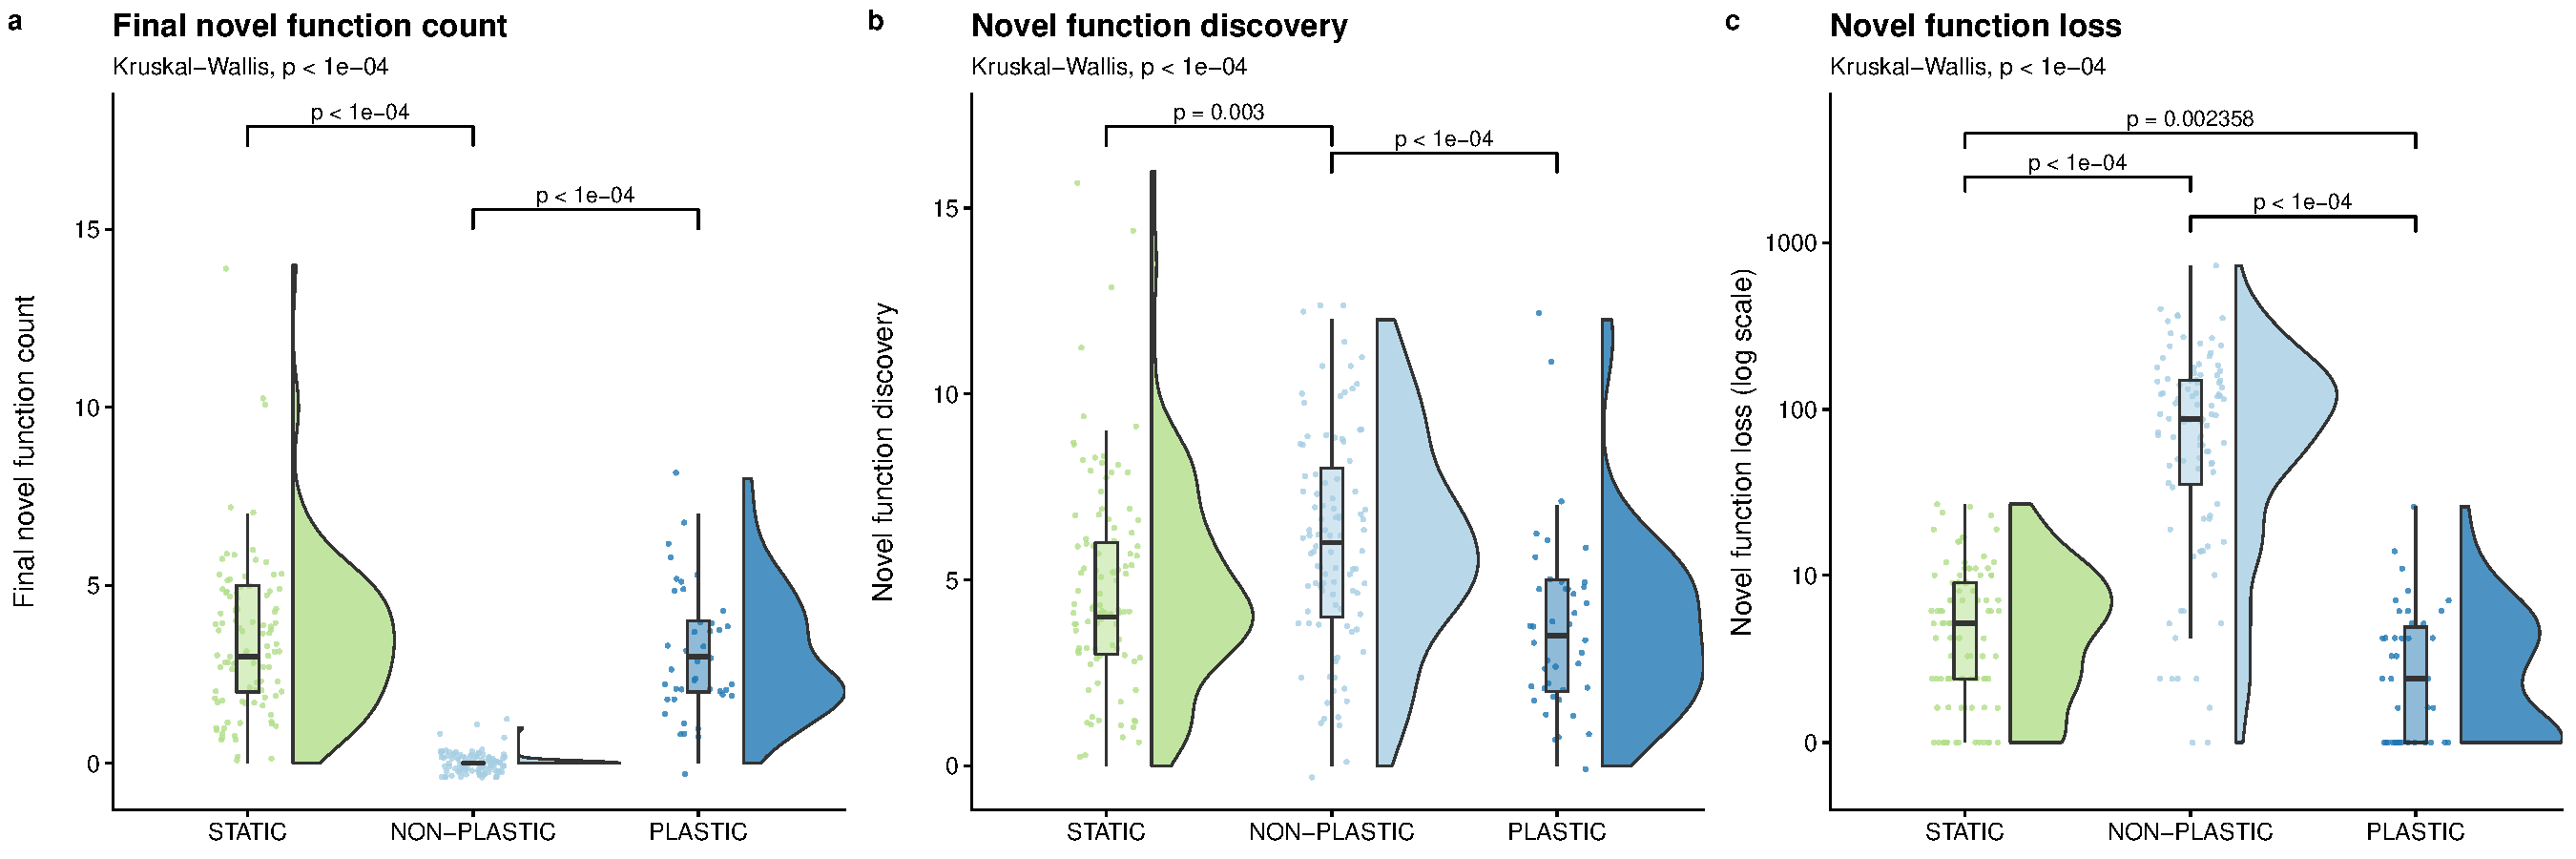
\includegraphics[width=0.9\textwidth]{05_consequences_of_plasticity/media/media-complex-traits-magnitude-panel.pdf}
  \caption{\small
  \textbf{Novel function evolution.}
  Raincloud plots of
  (a) final novel function count,
  (b) novel function discovery,
  and (c) novel function loss.
  See Table \ref{tab:metrics-definitions} for descriptions of each metric.
  Each plot is annotated with statistically significant comparisons (Bonferroni-corrected pairwise Wilcoxon rank-sum tests).
  Note that adaptive phenotypic plasticity evolved in \novelTraitsPlasticReps\ of \novelTraitsReplicates\ replicates from the PLASTIC treatment during phase one of this experiment; we used this more limited group to seed the resulting \novelTraitsPlasticReps\ phase-two PLASTIC replicates.
  }
  \label{fig:complex-traits-magnitude}
\end{figure}

% -- What did we test? --
We have so far shown that adaptive plasticity constrains the rate of evolutionary change in fluctuating environments.
However, it is unclear how this dynamic influences the evolution of novel functions.
Based on their relative rates of evolutionary change, we might expect NON-PLASTIC-treatment populations to evolve more novel functions than PLASTIC-treatment populations.
But, how much of the evolutionary change in NON-PLASTIC populations is useful for exploring novel regions of the fitness landscape versus continually rediscovering the same regions?

% - Magnitude of exploration/exploitation -
To answer this question, we quantified the number of novel functions performed by a representative organism in the final population of each replicate.
We found that both PLASTIC and STATIC populations had significantly higher final function counts than NON-PLASTIC populations at the end of the experiment (Figure~\ref{fig:complex-traits-magnitude}a).
The final novel function count in PLASTIC and STATIC lineages could be higher than that of the NON-PLASTIC lineages for several non-mutually exclusive reasons.
One possibility is that PLASTIC and STATIC lineages could be exploring a larger area of the fitness landscape when compared to NON-PLASTIC lineages.
Another possibility is that the propensity of the NON-PLASTIC lineages to maintain novel traits could be significantly lower than PLASTIC or STATIC lineages.
When we looked at the total sum of novel functions discovered by each of the PLASTIC, STATIC, and NON-PLASTIC lineages, we found that NON-PLASTIC lineages generally explored a larger area of the fitness landscape (Figure~\ref{fig:complex-traits-magnitude}b).
Although the NON-PLASTIC lineages discovered more novel functions, those lineages also exhibited significantly higher novel function loss when compared to PLASTIC and STATIC lineages (Figure~\ref{fig:complex-traits-magnitude}c).

\begin{figure}[h!]
  \centering
  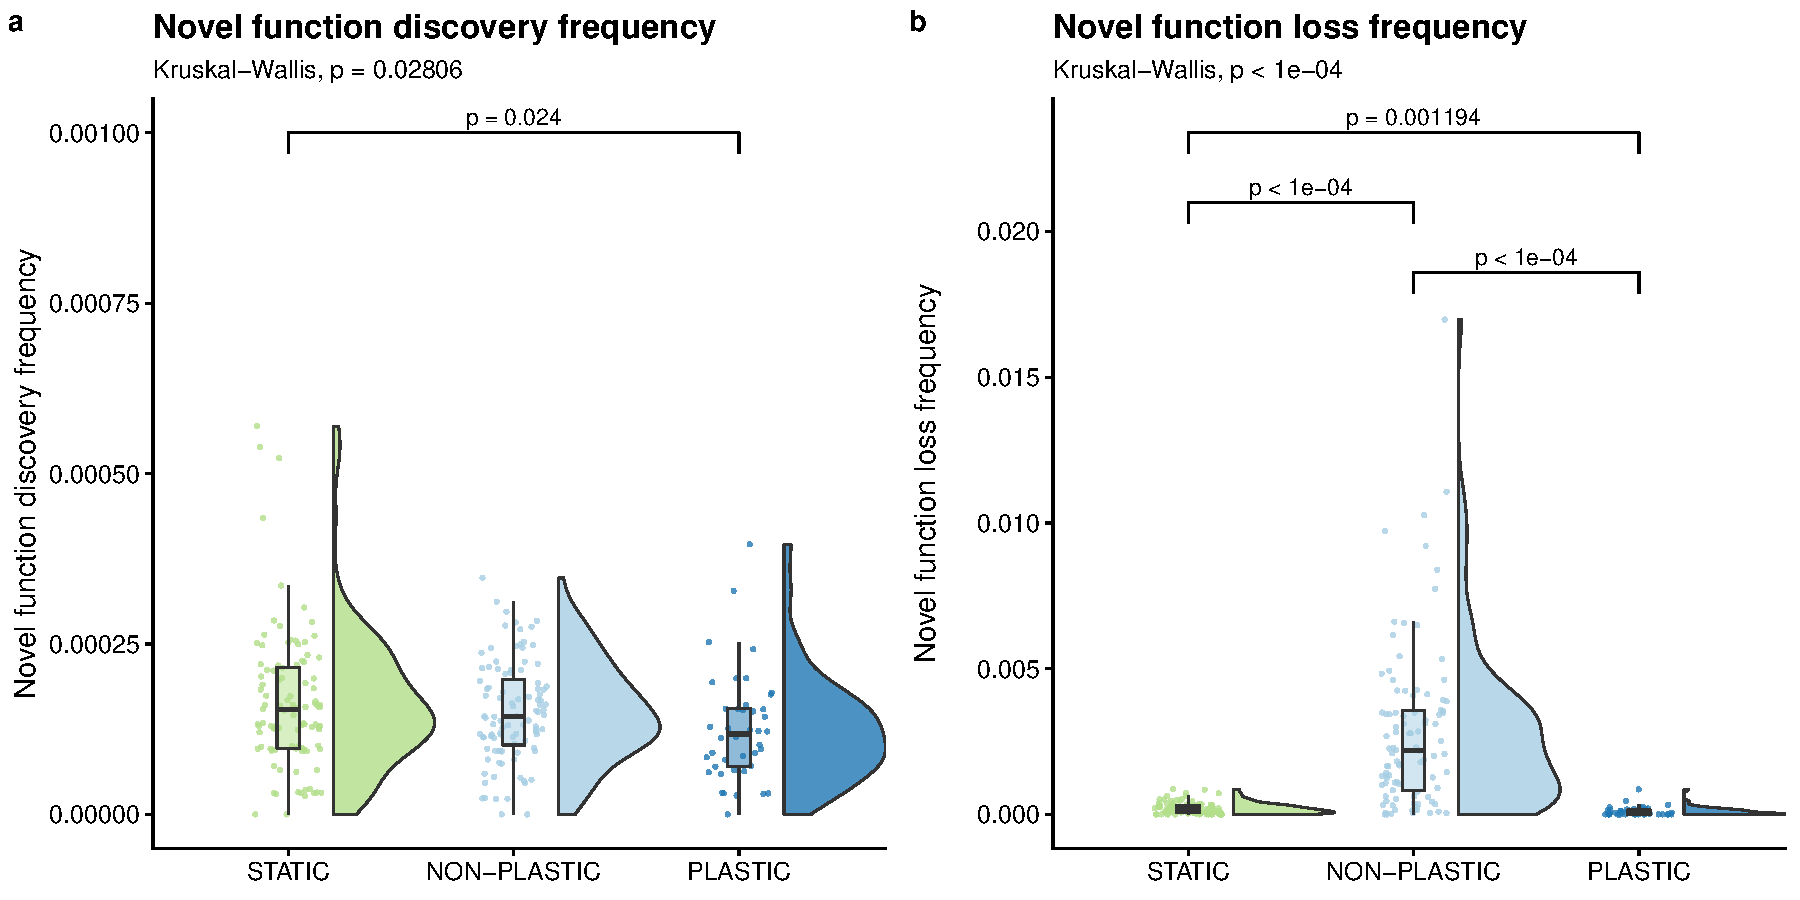
\includegraphics[width=0.66\textwidth]{05_consequences_of_plasticity/media/media-complex-traits-pace-panel.pdf}
  \caption{\small
  \textbf{Rate of novel function evolution.}
  Raincloud plots of
  (a) novel function discovery frequency
  and (b) novel function loss frequency.
  Each plot is annotated with statistically significant comparisons (Bonferroni-corrected pairwise Wilcoxon rank-sum tests).
  }
  \label{fig:complex-traits-rate}
\end{figure}

% - Rates of exploration/exploitation -
A larger number of generations elapsed in NON-PLASTIC populations than in PLASTIC or STATIC populations during our experiment \citep{supplemental_material}.
Are NON-PLASTIC lineages discovering and losing novel functions more frequently than PLASTIC or STATIC lineages, or are our observations a result of differences in generational turnover?
To answer this question, we converted the metrics of novel function discovery and novel function loss to rates by dividing each metric by the number of elapsed generations along the associated representative lineages.
We found no significant difference in the frequency of novel function discovery between NON-PLASTIC and STATIC lineages, and we found that PLASTIC lineages had a lower frequency of novel function discovery than STATIC lineages (Figure~\ref{fig:complex-traits-rate}a).
Therefore, we cannot reject the possibility that the larger magnitude of function discovery in NON-PLASTIC lineages was driven by a larger number of elapsed generations.
NON-PLASTIC lineages had a higher frequency of function loss than either PLASTIC or STATIC lineages, and PLASTIC lineages tended to have a lower frequency of novel function loss than STATIC lineages (Figure~\ref{fig:complex-traits-rate}b).


% - Characterizing trait loss -
Next, we examined the frequency at which novel function loss along lineages co-occurred with the loss or gain of any of the six base functions.
Across all NON-PLASTIC representative lineages, over 97\% (10998 out of 11229) of instances of novel function loss co-occurred with a simultaneous change in base function profile.
In contrast, across all PLASTIC and STATIC dominant lineages, we observed that approximately 20\% (29 out of 142) and 2\% (13 out of 631), respectively, of instances of novel function loss co-occurred with a simultaneous change in base function profile.
As such, the losses of novel functions in NON-PLASTIC lineages appear to be primarily due to hitchhiking or epistatic effects where a mutation that knocks out a maladaptive base function (after the environment changes) also knocks out a beneficial novel function.

\subsection{Lineages without plasticity that evolve in fluctuating environments express more deleterious functions}

%%%%%%
% 2021-02-05 - Results
% - Number of offspring on lineage where hitchhiker instruction execution increases (i.e., instances of hitchhiking)
%   - PLASTIC ~~ STATIC < NON-PLASTIC
% - Hitchhiker instruction increases / offspring on lineage
%   - PLASTIC ~~ STATIC < NON-PLASTIC
% - What fraction of mutations that increase hitchhiker instruction execution co-occur with base trait changes?
%   - NON-PLASTIC > PLASTIC ~~ STATIC
% - What about unexpressed vs expressed trait changes in plastic populations? (plastic only)
%   - Not much hitchhiking. Did not find evidence that hitchiking occurring as cryptic variation in unexpressed phenotype.
%%%%%%

Phenotypic plasticity allows for genetic variation to accumulate in genomic regions that are unexpressed, which could lead to the fixation of deleterious instructions in PLASTIC populations.
However, in NON-PLASTIC lineages, we observe a higher rate of novel function loss, indicating that they may be more susceptible to deleterious mutations (Figure \ref{fig:complex-traits-rate}b).

Therefore, in experiment phase 2C, we tested whether adaptive phenotypic plasticity can increase the incidence of deleterious function performance.
Specifically, we added an instruction that triggered an explicitly deleterious  function and measured the number of times it was executed.
Each execution of the \code{deleterious} instruction reduces an organism's fitness by 10\%.
At the beginning of phase 2C, the \code{deleterious} instruction is not present in the population, as it was not part of the instruction set during phase one of evolution.
Accordingly, if a \code{deleterious} instruction fixes in a population, it must be the result of evolutionary dynamics during phase 2C, including cryptic variation, hitchhiking, or as a result of sign epistasis where a \code{deleterious} instruction knocks out an even more maladaptive trait.
% sign epistasis; two things that are deleterious that are less deleterious in combination than you would expect form individual effects
% sign epistasis 

\begin{figure}[ht!]
  \centering
  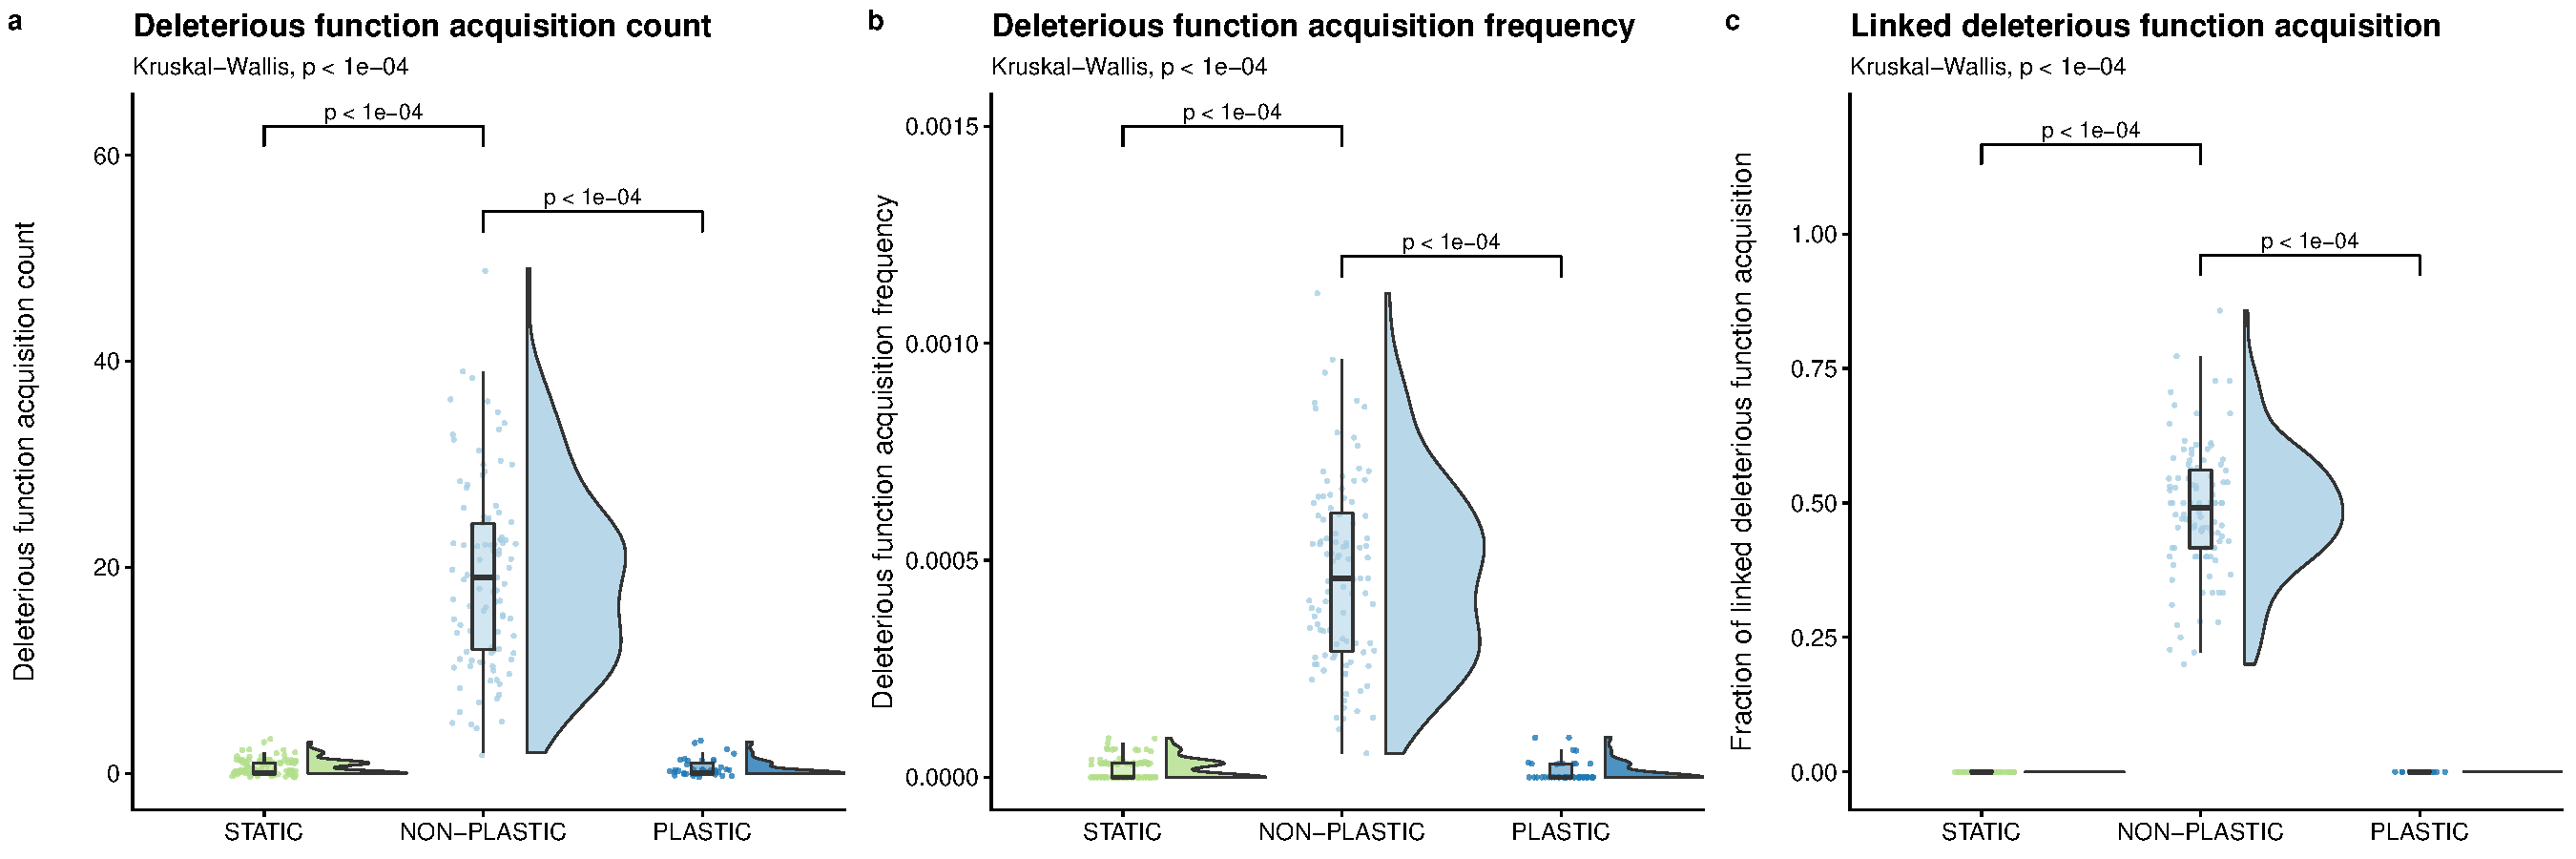
\includegraphics[width=1.0\textwidth]{05_consequences_of_plasticity/media/media-poison-accumulation-panel.pdf}
  \caption{\small
  \textbf{Deleterious instruction accumulation.}
  Raincloud plots of
  (a) deleterious function acquisition,
  (b) deleterious function acquisition frequency,
  and (c) the proportion of mutations that increase deleterious function expression along a lineage that co-occur with a change in phenotypic profile.
  Each plot is annotated with statistically significant comparisons (Bonferroni-corrected pairwise Wilcoxon rank-sum tests).
  Note that adaptive phenotypic plasticity evolved in \deleteriousHitchhikingPlasticReps\ of \deleteriousHitchhikingReplicates\ replicates from the PLASTIC treatment during phase one of this experiment; we used this more limited group to seed the \deleteriousHitchhikingPlasticReps\ phase-two PLASTIC replicates.
  }
  \label{fig:deleterious-hitchhiking}
\end{figure}

% -- Instruction execution by final dominant & along lineage --
At the end of our experiment, no representative organisms from the PLASTIC or STATIC treatments performed the deleterious function under any environmental condition; however, representative organisms in 14\% of replicates of the NON-PLASTIC treatment performed the deleterious function at least once.
NON-PLASTIC lineages contained significantly more mutations that conferred the deleterious function as compared to PLASTIC or STATIC lineages (Figure \ref{fig:deleterious-hitchhiking}a), and these mutations occurred at a significantly higher frequency in NON-PLASTIC lineages (Figure \ref{fig:deleterious-hitchhiking}b).
% Additionally, we did not observe
% This result does not change when we normalize [what?] by the number of generations represented in the given lineage (Figure \ref{fig:deleterious-hitchhiking}b).

% -- When/where does hitchhiking take place? --
Next, we measured how often mutations that increased deleterious function performance co-occurred with changes to the base function profile within representative lineages.
A \code{deleterious} instruction can fix in a population by having a beneficial effect that outweighs its inherent cost (\textit{e.g.}, knocking out a punished function) or through linkage with a secondary beneficial mutation at another site within the genome.
Across all NON-PLASTIC representative lineages, we found that approximately 49\% (956 out of 1916) of mutations that increased deleterious function expression co-occurred with a change in the base function profile (Figure \ref{fig:deleterious-hitchhiking}c).
In all representative lineages from the PLASTIC treatment, only 18 mutations increased deleterious function expression, and none co-occurred with a change in base function profile (Figure \ref{fig:deleterious-hitchhiking}c).
Likewise, only 58 mutations increased deleterious function performance in all representative lineages from the STATIC treatment, and none co-occurred with a change in base function profile (Figure \ref{fig:deleterious-hitchhiking}c).
We did not find compelling evidence that the few mutations that increased deleterious function expression occurred as cryptic variation in PLASTIC lineages.

We repeated this experiment with 3\% and 30\% metabolic rate penalties associated with the deleterious function, which produced results that were consistent with those reported here \citep{supplemental_material}.


% GUIDELINES:
% This section may be divided by subheadings. Discussions should cover the key findings of the study: discuss any prior research related to the subject to place the novelty of the discovery in the appropriate context, discuss the potential shortcomings and limitations on their interpretations, discuss their integration into the current understanding of the problem and how this advances the current views, speculate on the future direction of the research, and freely postulate theories that could be tested in the future.

\section{Discussion}

In this work, we used evolving populations of digital organisms to determine how adaptive phenotypic plasticity alters subsequent evolutionary dynamics and influences evolutionary outcomes in fluctuating environments.
Specifically, we compared lineages of adaptively plastic organisms in fluctuating environments to both non-plastic organisms in those same environments and other non-plastic organisms in static environments.

\subsection{Evolutionary change}

% -- Adaptively plastic populations underwent less evolutionary change than non-plastic populations --
We found strong evidence that adaptive plasticity slows evolutionary change in fluctuating environments.
Adaptively plastic populations experienced fewer coalescence events and fewer total genetic changes relative to non-plastic populations evolving under identical environmental conditions (Figure \ref{fig:evolutionary-dynamics-magnitude}).
Whereas non-plastic populations relied on \textit{de novo} mutations to adapt to each environmental fluctuation, plastic populations leveraged sensory instructions to regulate function performance.
Indeed, in fluctuating environments, selection pressures toggle after each environmental change.
We hypothesize that in non-plastic populations such toggling would repeatedly drive the fixation of mutations that align an organism's phenotypic profile to the new conditions.
This hypothesis is supported by the increased frequency of coalescence events in these populations (Figure \ref{fig:evolutionary-dynamics-rate}a) as well as increased rates of genetic and phenotypic changes observed along the lineages of non-plastic organisms.

% - Mutational neighborhood results
Representative lineages in the non-plastic treatment experienced lower realized mutational robustness than plastic and static lineages (Figure~\ref{fig:evolutionary-dynamics-rate}b).
We reasoned that this lower realized mutational robustness was due to non-plastic populations evolving a bet-hedging strategy where mutations are more likely to modify the phenotypic profile.
However, when we switched from measuring the realized mutational robustness of representative lineages to measuring the mutational robustness of representative genotypes (\textit{i.e.}, what fraction of one-step mutants change the phenotypic profile), we observed that non-plastic genotypes exhibited the highest mutational robustness of all three treatments (Figure~\ref{fig:mutational-robustness}).
This result runs contrary to both our expectations and the results of other fluctuating environment studies in Avida~\citep{canino-koning_fluctuating_2019}.
\cite{canino-koning_fluctuating_2019} found that mutational robustness is negatively correlated with the number of function-encoding sites in the genome.
In our work, most plastic and static genotypes encode all six base functions, while most non-plastic genotypes only encode functions from one environment; this results in fewer function-encoding sites, which may increase mutational robustness in non-plastic genotypes (relative to plastic and static genotypes). %relative to genotypes from other treatments.
Regardless of the cause, this higher mutational robustness in non-plastic organisms indicates that bet-hedging is not driving the low realized mutational robustness observed in non-plastic lineages.
Thus, we expect the lower realized mutational robustness in non-plastic lineages to be driven by survivorship bias.
Because non-plastic lineages must rely on mutations to adapt to environmental changes, phenotype-altering mutations are often highly advantageous, and their selection decreases the realized mutational robustness of successful lineages.


% -- in context of previous digital evolution work --
To our knowledge, this study is the first in-depth empirical investigation into how the \textit{de novo} evolution of adaptive plasticity shifts the course of subsequent evolution in a cyclic environment.
The relative rates of evolutionary change that we observed in non-plastic populations, however, are consistent with results from previous digital evolution studies.
For example, \cite{dolson_interpreting_2020} showed that non-plastic populations that were evolved in cyclically changing environments exhibited higher phenotypic volatility and accumulated more mutations than that of populations evolved under static conditions.
Furthermore, \cite{lalejini_evolutionary_2016} visually inspected the evolutionary histories of non-plastic organisms evolved in fluctuating environments, observing that mutations along successful lineages readily switched the set of traits expressed by offspring.
%\cite{canino-koning_evolution_2016} also observed that genomes evolved in harsh cyclic environments often contained vestigial fragments of genetic material adapted to prior environments.


% -- In context of conventional evolutionary theory: evo response => f(selection, variation) --
Our results are also consistent with conventional evolutionary theory.
A trait's evolutionary response to selection depends on the strength of directional selection and on the amount of genetic variation for selection to act upon \citep{lande_measurement_1983,zimmer_evolution_2013}.
In our experiments, non-plastic populations repeatedly experienced strong directional selection to toggle which functions were expressed after each environmental change.
As such, retrospective analyses of successful lineages revealed rapid evolutionary responses (that is, high rates of genetic and phenotypic changes).
Evolved adaptive plasticity shielded populations from strong directional selection when the environment changed by eliminating the need for a rapid evolutionary response to toggle function expression.
Indeed, both theoretical and empirical studies have shown that adaptive plasticity can constrain evolutionary change by weakening directional selection on evolving populations \citep{price_role_2003,paenke_influence_2007,ghalambor_non-adaptive_2015}.

% TODO, consider: Expectations that could arise if we took into consideration lineages off the line of descent.

\subsection{The evolution and maintenance of novel functions}

% -- Exploration + Exploitation --
In fluctuating environments, non-plastic populations explored a larger area of the fitness landscape than adaptively plastic populations (Figure \ref{fig:complex-traits-magnitude}b).
However, adaptively plastic populations better exploited the fitness landscape, retaining a greater number of novel functions than non-plastic populations evolving under identical environmental conditions (Figure \ref{fig:complex-traits-magnitude}a).
In our experiment, novel functions were less important to survival than the fluctuating base functions.
In non-plastic populations, when a mutation changes a base function to better align with current environmental conditions, its benefit will often outweigh the cost of losing one or more novel functions.
Indeed, we found that along non-plastic representative lineages, 97\% of the mutations associated with novel function loss co-occurred with phenotypic changes that helped offspring adapt to current environmental conditions.

% -- Changing environments promote evolutionary change --
Previous studies have shown that transitory environmental changes can improve overall fitness landscape exploration in evolving populations of non-plastic digital organisms \citep{nahum_improved_2017}.
Similarly, changing environments have been shown to increase the rate of evolutionary adaptation in simulated network models \citep{kashtan2007varying}.
In our system, however, we found that \textit{repeated} fluctuations reduced the ability of non-plastic populations to maintain and exploit functions; that said, we did find that repeated fluctuations may improve overall function discovery by increasing generational turnover.
Consistent with our findings, \cite{canino-koning_fluctuating_2019} found that non-plastic populations of digital organisms evolving in a cyclic environment maintained fewer novel traits than populations evolving in static environments.

% -- Plastic rescue, stabilizing effect of plasticity --
Our results suggest that adaptive phenotypic plasticity can improve the potential for populations to exploit novel resources by stabilizing them against stressful environmental changes.
The stability that we observe may also lend some support to the hypothesis that phenotypic plasticity can rescue populations from extinction under changing environmental conditions \citep{chevin_adaptation_2010}.

% -- relevance to genes as followers hypothesis --.
Our data do not necessarily provide evidence for or against the genes as followers hypothesis.
The genes as followers hypothesis focuses on contexts where plastic populations experience novel or abnormally stressful environmental change.
However, in our system, environmental changes were cyclic (not novel), and no single environmental change was \textit{abnormally} stressful.
Further, the introduction of novel functions during the second phase of the experiment merely added static opportunities for fitness improvement.
This addition did not change the meaning of existing environmental cues, nor did it require those cues to be used in new ways.

\subsection{The accumulation of deleterious alleles}

% -- Overview of results --
%   - More accumulation in non-plastic
%   - no evidence for cryptic variation housing poison
%   - plastic ~~ static
We found that non-plastic lineages that evolved in a fluctuating environment exhibited both greater totals and higher rates of deleterious function acquisition than that of adaptively plastic lineages (Figure \ref{fig:deleterious-hitchhiking}).
There are several, non-mutually exclusive possibilities that could explain the fixation of explicitly deleterious instructions: random genetic drift, deleterious hitchhiking, epistatic effects, and cryptic variation (in plastic organisms).
We find it unlikely that random genetic drift explains our observations.
Each time an organism expresses a \code{deleterious} instruction, the organism incurs a 10\% penalty to their replication rate, which results in strong purifying selection against mutations that cause offspring to execute \code{deleterious} instructions.

In asexual populations without horizontal gene transfer, all co-occurring mutations are linked.
As such, deleterious mutations linked with a stronger beneficial mutation (\textit{i.e.}, a driver) can sometimes ``hitchhike'' to fixation \citep{smith_hitch-hiking_1974,van_den_bergh_experimental_2018,buskirk_hitchhiking_2017}.
Natural selection normally prevents deleterious mutations from reaching high frequencies, as such mutants are outcompeted.
However, when a beneficial mutation sweeps to fixation in a clonal population, it carries along any linked genetic material, including other beneficial, neutral, or deleterious mutations \citep{barton_genetic_2000, smith_hitch-hiking_1974}.
Therefore, deleterious genetic hitchhiking could have contributed to \code{deleterious} instruction accumulation along non-plastic lineages in changing environments.

% Antagonistic pleiotropy occurs when a mutation has beneficial effects for one trait but also causes deleterious effects on other traits~\citep{zimmer_evolution_2013}. 
Epistatic effects (\textit{i.e.}, interactions between genes) could have also contributed to \code{deleterious} instruction accumulation along non-plastic lineages. 
On their own, mutations that increase \code{deleterious} instruction execution are maladaptive; however, if such a mutation were to also knock out an even more harmful function, that mutation may have a net beneficial effect.
As such, mutations that confer increased \code{deleterious} instruction execution could directly drive a selective sweep. 

% Across our experiments, the frequency of selective sweeps in non-plastic populations provided additional opportunities for genetic hitchhiking and antagonistic pleiotropy with each environmental change.
% Indeed, 
Representative lineages from non-plastic populations in the cyclic environment exhibited higher mutation accumulation (Figure~\ref{fig:evolutionary-dynamics-magnitude}b), novel function loss (Figure~\ref{fig:complex-traits-magnitude}c), and deleterious function acquisition (Figure~\ref{fig:deleterious-hitchhiking}a) than their plastic counterparts.
In aggregate, we found that many ($\sim$49\%; 956 / 1916) mutations that increased \code{deleterious} instruction execution in offspring co-occurred with mutations that provided an even stronger benefit by adapting the offspring to an environmental change.
We expect that an even larger fraction of these deleterious mutations were linked to beneficial mutations, but our analysis only counted mutations that co-occurred in the same generation.
Our analyses did not distinguish between epistatic effects and deleterious hitchhiking; however, more fine-grained analyses of secondary effects of mutations that conferred \code{deleterious} instruction execution could be performed in future work to disentangle these two mechanisms.


% -- Elaboration on plastic result --
Theory predicts that under relaxed selection deleterious mutations should accumulate as cryptic variation in unexpressed traits \citep{lahti_relaxed_2009}.
Contrary to this expectation, we did not find evidence of \code{deleterious} instructions accumulating as cryptic variation in adaptively plastic lineages.
One possible explanation is that the period of time between environmental changes was too brief for variants carrying unexpressed \code{deleterious} instructions to drift to high frequencies before the environment changed, after which purifying selection would have removed such variants.
Indeed, we would not expect drift to fix an unexpressed trait since we tuned the frequency of environmental fluctuations to prevent valuable traits from being randomly eliminated during the off environment.
Additionally, plastic organisms in Avida usually adjust their phenotype by toggling the expression of a minimal number of key instructions, leaving little genomic space for cryptic variation to accumulate.

\subsection{Limitations and future directions}

% ------------
% Possible additional future directions:
% - Need to look at mutations off the line of descent
% - Variable length genomes
% - Relaxed selection, mutational decay
% ------------

% -- Adaptive vs non-adaptive plasticity --
Our work lays the groundwork for using digital evolution experiments to investigate the evolutionary consequences of phenotypic plasticity in a range of contexts.
However, the data presented here are limited to the evolution of \textit{adaptively} plastic populations.
Future work might explore the evolutionary consequences of maladaptive and non-adaptive phenotypic plasticity (\textit{e.g.}, \citealt{leroi_temperature_1994}), which are known to bias evolutionary outcomes~\citep{ghalambor_non-adaptive_2015}.

% -- Environmental change --
Additionally in our experiments, sensory instructions perfectly differentiated between ENV-A and ENV-B, and environmental fluctuations never exposed populations to entirely new conditions.
These parameters have been shown to influence evolutionary outcomes~\citep{li_digital_2004,boyer_adaptation_2021}, which if relaxed in the context of further digital evolution experiments, may yield additional insights.
Our experiments also focused on asexually reproducing digital organisms. 
Sexual reproduction has been shown to be advantageous in rapidly changing environments, such as the cyclic environments used in our study~\citep{misevic_experiments_2010}. 
Future work could investigate how sexual reproduction affects the evolutionary consequences of adaptive plasticity. 

% - limitation: focus on lineages -
%   - extend to complete evolutionary histories
We focused our analyses on the lineages of organisms with the most abundant genotype in the final population.
These successful lineages represented the majority of the evolutionary histories of populations at the end of our experiment, as populations did not exhibit long-term coexistence of different clades.
Our analyses, therefore, gave us an accurate picture of what fixed in the population.
We did not, however, examine the lineages of extinct clades.
Future work will extend our analyses to include extinct lineages, giving us a more complete view of evolutionary history, which may allow us to better distinguish adaptively plastic populations from populations evolving in a static environment.

% - Machinery -
As with any wet-lab experiment, our results are in the context of a particular model organism: ``Avidian'' self-replicating computer programs.
Digital organisms in Avida regulate responses to environmental cues using a combination of sensory instructions and conditional logic instructions (\code{if} statements).
The \code{if} instructions conditionally execute a single instruction depending on previous computations and the state of memory.
As such, plastic organisms in Avida typically regulate phenotypes by toggling the expression of a small number of key instructions as opposed to regulating cohorts of instructions under the control of a single regulatory sequence \citep{supplemental_material}.
This bias may limit the accumulation of hidden genetic variation in Avida genomes.
However, as there are many model biological organisms, there are many model digital organisms that have different regulatory mechanisms (\textit{e.g.}, \citealt{lalejini_evolving_2018}) that should be used to test the generality of our results.

% -- Reviewer 1 comment --
% With a population size of 3600 individuals and a genomic mutation rate of 0.25 mutations/genome/generation, potential beneficial mutations are generated quickly and selective sweeps occur quickly
% "One can imagine that a larger population with a decreased mutation rate would not see the observed phenomenon due to differences in the dynamics of selective sweeps."
% "Altering the time spent in each environment may alter this trend of selective sweeps driving deleterious mutation accumulation. "
As with most digital evolution experiments, our mutation rates were high and population sizes were small (3600 individuals) relative to experiments with microbes or conditions common in nature.
As such, beneficial mutations can be generated rapidly and selective sweeps can occur quickly.
Moreover, our analyses were limited to a single rate of environmental change and simple function reward structures, which likely influenced the rates of selective sweeps observed in our experiments. 
Future studies could address these limitations by increasing population sizes, decreasing mutation rates, investigating different function rewards and punishments, and altering the time spent in each environment. %, painting a more complete picture of the range of scenarios where our results apply.


\end{raggedbottom}

\section*{Supplemental Material}

The supplemental material for this article is hosted on GitHub and can be found online at \url{https://github.com/amlalejini/evolutionary-consequences-of-plasticity} \citep{supplemental_material}.

\section*{Data Availability Statement}

The datasets generated and analyzed for this study can be found on the Open Science Framework at \url{https://osf.io/sav2c/} \citep{osf_data}.
%\chapter{Proposed -  The potentiation of memory and other complex features}
\chapter{Proposed -  Patterns in potentiation across multiple environments}
\label{chap:varying_environments}

\noindent
Authors: Austin Ferguson, Anselmo Pontes, and Charles Ofria

\noindent
Status: Proposed. %but all software has been developed as part of previous work.
%One environment comes from work that is currently only published as a chapter in Anselmo Pontes' dissertation \citep{pontesEvolutionaryOriginsCognition2021}. 
%The other environment is a variant of the Logic 9 environment used in Chapter \ref{chap:consequences_of_plasticity} to study plasticity. 
%I propose to study potentiation in two environments, both of which have been ported from Avida2 to MABE2 and are ready to be used. 
While data collection has not started, both environments I propose to explore have been ported from Avida2 to MABE2 and are ready to be used. 
%Part of this extension will focus on potentiation in the patch harvesting environment, looking at lineages that evolved the memory necessary to switch from consuming one patch to finding another. 
%This has all been implemented in Avida in MABE2, as well as the Logic 9 environment we use to replicate the plasticity environment seen in Chapter \ref{chap:varying_environments}.
% As we work to get the work ready to publish, I first re-implemented the system in the new, in-progress version of Avida with MABE2 and begun re-running all the data from the previous work. 
% My intellectual contribution is a deeper dive into the genotypes that heavily exploit a patch and then move on in search for a new patch. 
% While the previous work looked at one lineage, my plan is to look into \textit{all} lineages that exhibit this behavior. 
% Additionally, I plan to conduct analytic replay experiments on these lineages to see how the potentiation of patch-hopping behavior changed over time. 
 

\section{Introduction}

% Lead in - how does this relate to the other chapters
Previous work has shown that the environment can influence the relative contributions of adaptation, chance, and history \cite{smithFitnessEvolvingBacterial2022}. 
I have previously proposed testing how changes to the environment and underlying representation affect potentiation in successful lineages (Chapters \ref{chap:replaying_associative_learning} and \ref{chap:simplified_model}). 
However, I will be unable to concretely identify if differences between those two systems are due to changing the environment or the representation. 
To remedy this issue, here I propose to quantify potentiation along successful lineages in two additional Avida environments.
By keeping the representation constant, potentiation differences must therefore be a result of the change in environment or the targeted trait within. %due to the one factor that has changed, the environment. 

% The results of Chapters \ref{chap:replaying_associative_learning} and \ref{chap:simplified_model} are uncertain, but I expect one of three possibilities: %can have many potential outcomes, but we can boil them down to three categories: 
% 1) we observe similar patterns in potentiation between the associative learning Avida environment and the simplified bitstring model, 
% 2) potentiation looks drastically different between the two setups, with no discernible patterns, or
% 3) a mix, where some traits are shared and others are drastically different. 
% My hypothesis is that the third option is what we will observe. 
% However, regardless of which situation is true, the results of those chapters will lay the initial expectations for how potentiation varies as systems change. 
% Between those chapters I proposed to vary both the environment and the representation of organisms. 
% Here, I propose to lock the representation, analyzing potentiation in two additional environments within Avida. 

%Regardless of which situation is true, the results of those chapters will prompt us to look at the similarities and differences in potentiation between the two systems. 
%If there are differences, can we untangle \textit{why} these differences exist? 
%If the patterns are mostly the same, can we use this information to predict how potentiation will change when looking at other environments and target behaviors?
%These are the questions I propose to investigate in this chapter by looking at two different environments and target behaviors in Avida. 

%Avida has been used to study a wide variety of evolutionary dynamics, ranging from X to Y to Z. 

% Why stick with Avida? Easier comparisons with the same levels of epistasis. 
I hypothesize that in many cases, potentiating mutations are highly epistatic, as epistasis is one key way for a seemingly innocuous mutation to have a drastic effect on later mutations.
As such, studies of potentiation should employ representations capable of epistatic interactions. 
This is an advantage of using Avida; there are multiple possibilities for epistasis between instructions, and in previous work I have confirmed that these interactions are sufficient for complex potentiation dynamics (Chapter \ref{chap:alife_submission}).
By conducting studies of potentiation in multiple Avida environments, I will investigate how environmental differences influence potentiation as the underlying representation, and thus the potential for epistatic interactions, only slightly differ. 

%We have demonstrated in Chapter \ref{chap:alife_submission} that we can quantify how the potentiation of a target behavior changes along a successful lineage in Avida.
%By the time we start on this project, we will have observed potentiation at a larger scale (Chapter \ref{chap:replaying_associative_learning}) and in a simplified model (Chapter \ref{chap:simplified_model}). 
Specifically, I propose to investigate potentiation in a patch harvesting behavior and in phenotypic plasticity. 
In the patch harvesting environment described in \citep{pontesEvolutionaryOriginsCognition2021}, I will target the successful harvesting of multiple patches in an organism's lifetime. %memory usage in the decision to exploit the current patch or explore to find a new patch. 
In the cyclic logic 6 environment (Chapter \ref{chap:consequences_of_plasticity}), I will target optimal plasticity. 
%By changing the environments and the behaviors we consider successful, we will be analyzing very different fitness landscapes and the effects they have on potentiation. 
While both target behaviors are complex, their details differ both with each other and with associative learning from previous work (Chapter \ref{chap:replaying_associative_learning}). 
Ultimately, will these details influence how potentiation changes? 

% Expectations and impact
%Specifically, here we target two different yet related behaviors. 
The patch harvesting behavior I am targeting is a basic cognitive behavior. 
In order to harvest multiple patches, organisms must switch between exploring to find new patches or exploiting the patch they are currently on. % state in order to successfully harvest multiple patches. 
Similar to the associative learning behavior in Chapter \ref{chap:replaying_associative_learning}, this behavior requires several different components in order to function (information storage, memory retrieval and usage, etc.).
As such, I expect the two behaviors to exhibit similar patterns in potentiation. 
%Specifically, I expect that single mutations (especially in the formation and usage of memory) can result in a drastic potentiation increase. 
The other behavior, optimal plasticity in the cyclic logic 6 environment, is a reactive behavior that does not require memory. % has similarities and differences to the other two behaviors.
It does, however, still consist of multiple components (performing tasks and regulating them due to environmental cues) that can be neutral or deleterious in isolation. 
Therefore, I also expect to see similar patterns in potentiation in the evolution of optimal plasticity. % regardless of the difference in the behaviors. 

% Conclusion - this is important because regardless of what the outcome is, the information we gain will be incredibly useful for future studies into potentiation and the role of history in evolution
This work will expand upon the previous chapters, providing additional examples of how potentiation changes as we vary the environment and target behavior. 
All together, these works will shape how we view potentiation, and will provide an expanding dataset for other researchers to compare against in the future. 
% Note that this will be the first time incorporating what we learned from chapter 4?

% As we discussed in the previous chapters, we can quantify how potentiation, the likelihood a focal trait evolves from a given genotype, changes over time. 
% In those chapters, I proposed studying these changes in potentiation in the context of associative learning (Chapters \ref{chap:alife_submission} and \ref{chap:replaying_associative_learning}) and in a simple bitstring NK landscape model (Chapter \ref{chap:simplified_model}). 
% The goal of those chapters is to try and find common trends in how potentiation changes across multiple lineages. 
% Here we continue to expand on these questions by looking at potentiation of different behaviors in two other environments: microbial mat harvesting seen by early bilaterian animals and the classic Logic 9 Avida environment. 

% This chapter asks if the target behavior influences how potentiation changes over time given a fixed substrate (in this case Avida organisms). 
% We will conduct replay experiments on successful lineages from both environments, applying insights learned from the bitstring model of Chapter \ref{chap:simplified_model}, to see if any general patterns emerge. 
% If we do not see general trends in the evolution of different behaviors in Avida, that will be strong evidence that potentiation is very unique to the target behavior we are analyzing. 
% If we \textit{do} see general trends, however, this work (along with the previous chapters) will lay the groundwork for future studies in other environments, computational substrates, or even in living organisms. 
\section{Methods}

Here I describe the two environments and the behaviors that we are targeting within them. 

\subsection{The patch harvesting environment}

% What are we modeling?
The first environment aims to model the patch harvesting behavior of early bilaterians as they traversed microbial mats. 
Fossil records of the paths taken by these animals provide evidence of complex behavioral patterns, potentially resulting from early cognitive behaviors \citep{carboneWhenLifeGot2014}. 
This environment is a re-implementation of the one found in \citep{pontesEvolutionaryOriginsCognition2021}. 
In this environment, organisms are rewarded for consuming nutrients and punished for time spent off the patch. 
Here, we specifically look at environments with multiple patches of nutrients, and our target behavior is the successful consumption of multiple patches. 
This behavior requires switching between at least two tasks (exploring or exploiting), and as such, it is a cognitive behavior comparable to associative learning in Chapter \ref{chap:replaying_associative_learning}.
%This behavior requires memory to solve, and as such it presents a testbed for a cognitive behavior that is comparable to associative learning in previous work. 
%aim to quantify the potentiation of memory usage required to switch between exploiting one patch and exploring to find a new patch. 

% General overview of how the environment is used
Our Avida organisms exist in the typical 60x60 toroidal grid, with parent organisms replicating into a neighboring cell. 
The evaluation of the organisms, however, occurs on a toroidal, two-dimenstional spatial grid that represents microbial mats like those encountered by the early bilaterians. 
These environments consist of various patterns of nutrients that the organisms can consume and empty tiles whose traversal causes the organisms to waste energy. 

% How does the environment actually work?
To facilitate the consumption of nutrients, organisms are granted four new instructions to navigate their environment. 
Movement is accomplished via three instructions: \texttt{Turn Left}, \texttt{Turn Right}, and \texttt{Move Forward}. 
The right and left instructions rotate the organism 45 degrees in the appropriate direction. 
The move instruction always moves the organism a single tile in the direction it is pointing, including diagonally. 
Finally, the organisms are given a \texttt{Sense} instruction to pull information from their environment. 
Specifically, the sense instruction will give the organism a numeric cue depending on what floor tile it is currently on. 
%Nutrient tiles result in a 3 cue, while 
Empty tiles return a negative one, while already-consumed nutrient tiles result in positive one. 
Nutrients are consumed as the organism moves onto that tile without requiring an additional action, and as such organisms will never sense a nutrient tile that has not been consumed.  

% How does scoring work? 
Organisms are scored based on how well they consume nutrients and avoid empty tiles. 
The organism's score is increased by one for each nutrient consumed. 
For every empty tile visited, however, the organism's score is reduced by one to model the organism expending energy to move for no nutrient gain. 
Moving onto a previously-consumed tile has no effect on score, as if some residual nutrients could offset the energy consumption. 
Finally, as is often done in Avida, this score is used in an exponential. 
The performance of the organism is calculated as $2^{\text{score}}$, which means an additional nutrient consumed always doubles performance, regardless of how many nutrients have been consumed in total. 
As is customary in Avida, this score is used to weight which organisms receive the most updates and thus execute their genomes faster. 

\begin{figure}
    \centering
    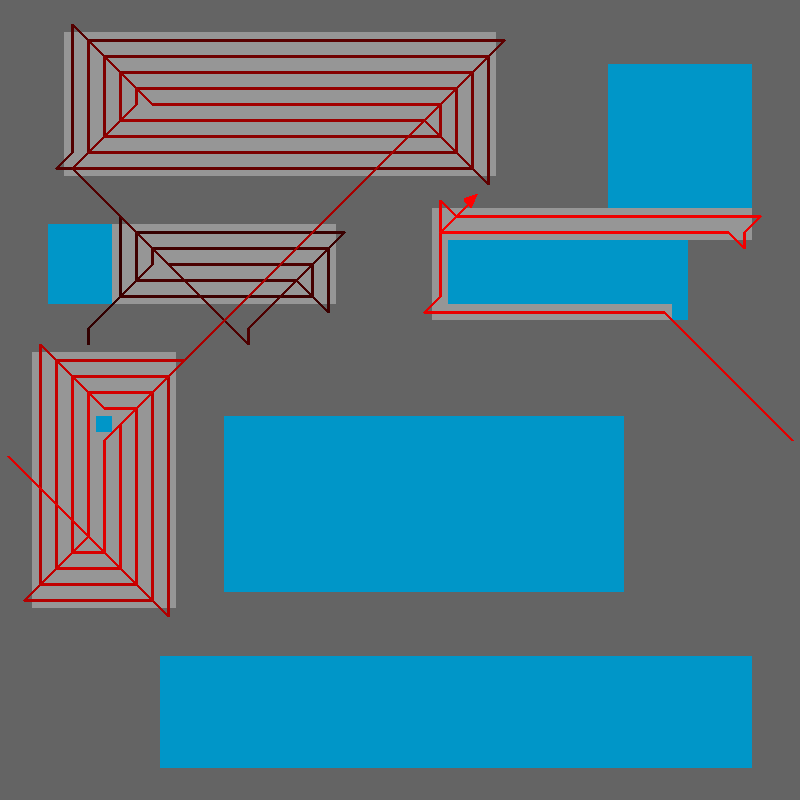
\includegraphics[width=0.9\textwidth]{06_memory_in_patch_harvesting/media/patch_harvest_example.png}
    \caption{
    An example layout of disconnected patches in the patch harvesting environment.
    Blue tiles represent food that has yet to be consumed, light gray tile are food that has been consumed, and dark gray tiles show empty space which is costly to move into. 
    The lines show the trace of an evolved organism (red triangle), with the start of the line in black and a slow fade to red as the trace becomes more recent. 
    This organism has evolved a spiraling behavior and has successfully consumed three patches of food. 
    }
    \label{fig:patch_harvest:example}
\end{figure}

% For more example images, see seeds 27, 31, and 32 for disconnected patches without edges

% Discussion of the target behavior and why it's cool
While previous work has used multiple patch types \citep{pontesEvolutionaryOriginsCognition2021}, here I propose to study only one: multiple disconnected patches.
The smaller patches in this environment require organisms to switch patches once they have exploited their current patch in order to maximize their score. 
These two behaviors (exploration and exploitation) can be thought of as two states the organism can be in.
As such, I expect this behavior to require memory, as a single bit of information is needed to store what state the organism is in. 
% The organism must determine when it has successfully consumed a patch and then move to find a new patch to eat. 
% This requires at least two states of behavior. 
Figure \ref{fig:patch_harvest:example} shows an example of the disconnected patches, as well as an evolved organism's successful trace through the environment. 
To easily categorize organisms that are capable of consuming multiple patches, I will require the organism to have consumed at least half each of two patches to be considered a ''successful'' behavior. 
Exploratory work has shown that this behavior does evolve, but only rarely. 
In 200 initial replicates, it appeared in only nine. % replicates. 
%This rarity works in our favor, as rare behaviors have the most room for potentiation gain. 
Much like associative learning in previous work, this rarity provides substantial room for improvements in potentiation over the course of a lineage. 

\subsection{The cyclic logic 6 environment}

% Intro
There may be inherent similarities between the associative learning task of Chapters \ref{chap:alife_submission} and \ref{chap:replaying_associative_learning} and the cognitive behavior needed in the patch harvesting environment. 
As such, here I propose one final, non-cognitive environment to test potentiation: the cyclic environment from Chapter \ref{chap:consequences_of_plasticity}, which I will refer to here as ``cyclic logic 6''. 

% Overview of environment
The cyclic logic 6 environment in Avida consists of two sets of bitwise logic tasks: one that is rewarded and one that is punished. 
Which set is rewarded, however, switches at regular intervals. 
Each organism receives a set of random input numbers, and then has the opportunity to perform computations and eventually output these values.  %performs whatever computation on them, and potentially outputs one or more values. 
If output values are deemed to be a successful logic operation on one or more inputs, then the organism is rewarded or punished according to the current state of the environment.  
The Avida organisms, however, are only given access to a bitwise \texttt{NAND} instruction, which they must use to build the other logic operations. 
% The simplest two tasks, NOT and NAND, confer a reward of 2, while we increase to a reward of 4 for AND and ORNOT, 8 for ANDNOT and OR, 16 for XOR and NOR, and finally a reward of 32 for EQU. 
% Rewards are multiplicative, so performing NOT and XOR would result in a performance of 32. 
% Organisms are only rewarded once for each logic task they perform. 

% Explanation of cycling
At any given time, three of the six logic tasks will be rewarded while the other three are punished. 
In this cyclic environment, this reward scheme is flipped at regular intervals.
%When this flip occurs, tasks that were rewarded become punished and vice versa. 
%An organism's score is doubled when it performs a rewarded task for the first time and halved when performing a punished task for the first time. 
When performing a logic task for the first time, an organism's score is doubled if that task is rewarded or halved if the task is punished. 
Here I flip the rewards and punishments every 100 updates. 
I will give organisms access to a new instruction, \texttt{Sense}, so they can determine what environment they are in and can potentially regulate task expression accordingly.
This environment is described in detail in Chapter \ref{chap:consequences_of_plasticity}, though here I am only using the PLASTIC environment from Phase 1 (see Figure \ref{fig:experimental-design}, panels A and C). 
I will use the same two sets of tasks used in Chapter \ref{chap:consequences_of_plasticity} (NOT, AND, and OR) and (NAND, AND-NOT, OR-NOT).

% What is optimal plasticity?
Due to the cycling of which tasks are rewarded, organisms must exhibit optimal plasticity to maximize fitness. 
As in the previous chapter, I define optimal plasticity as performing the three rewarded tasks and zero of the punished tasks. 
While organisms are born into a particular environment, I will test for optimal plasticity \textit{post hoc}, evaluating the organism in both variations of the environment. 
Therefore, for an organism to exhibit optimal plasticity, they must be capable of perfectly regulating all six tasks depending on which environment they are in. 

% Optimal plasticity is our target behavior
It is this optimal plasticity that I will target for the potentiation analysis. 
Compared to associative learning and multi-patch harvesting behaviors, optimal plasticity is a much more common behavior to evolve from the ancestor, with Chapter \ref{chap:consequences_of_plasticity} seeing greater than 40\% of replicates evolve the behavior.
While it is may be more common, this behavior is still nontrivial. 
To perform optimal plasticity, organisms must be capable of performing all six logic tasks, sensing the environment, and using the environment data to regulate the execution of the logic tasks. 
This task, however, can be solved reactively; it is unnecessary to store the environment state in memory. 
Still, I expect the complex nature of the environment to translate into interesting patterns in potentiation, not unlike those of associative learning seen in previous work. 



% Logic 9 has been well-studied in Avida. 
% Previous work has looked into how different evolutionary dynamics factor into the evolutionary dynamics of the more complex logic tasks, specifically equals (EQU) [CITE]. 
% As such, EQU provides us with a difficult-to-evolve target behavior that we can use for our potentiation studies. 
% By running analytic replays on lineages that evolve EQU, we can see how their likelihood to evolve the behavior changed over time. 
% This behavior has the potential to be quite different from associative learning from previous chapters or memory usage in the previous environment, as EQU does not require any cognitive processes. 
% Thus, the potentiation of EQU will be a solid basis of comparison as a behavior that does not require memory but is still difficult to evolve. 
\section{Proposed work}

In both environments, I will measure attributes of potentiation by conducting analytic replay experiments as described in Chapter \ref{chap:replaying_associative_learning}. 
I will then compare the measurements to previous data from Chapters \ref{chap:replaying_associative_learning} and \ref{chap:simplified_model} to determine what differences exist between the different environments. 
This work will provide additional examples of potentiation and allow the first cross-environment comparisons while keeping the underlying representation the same. 

Potentiation will be quantified using the exact same methods as Chapter \ref{chap:replaying_associative_learning}. 
Initial evolutionary replicates seeded with the default ancestor will be conducted to find replicates that exhibit the target behavior (multi-patch harvesting or optimal plasticity). 
For each environment, I will run initial replicates until I reach 40 successful lineages. 
To measure the changes in potentiation along the dominant lineage of each replicate, I will conduct two phases of replay experiments. 
The first will seed replicates with the genotypes found 50, 100, 150, and 200 steps before the target behavior first appeared in the lineage. 
I will continue to go backward along the lineage until a step shows less than 10 percentage points of improvement over the success rate from the initial replicates.
Once the exploratory replays have been conducted, I will identify potentiation windows (as in Chapter \ref{chap:replaying_associative_learning}) and seed replay replicates for every genotype in the windows. 
As before, I will run fifty replay replicates for each genotype analyzed. 

After conducting the replay experiments, I will collect the same potentiation measures described in Section \ref{sub:potentiation_measures}.
%These include maximum single-step potentiation gain/loss, the number of potentiation gain/loss windows, the fitness effect and behavioral background of potentiating/anti-potentiating mutations, and the distance between potentiating mutations and the appearance of the target behavior. 
Since these are the same measurements recorded in Chapters \ref{chap:replaying_associative_learning} and \ref{chap:simplified_model}, I can then statistically compare the distributions of each measurement across environments. 
The one exception is the behavioral background, which is unique to each task and thus can only be compared within a given environment. 
The cross-environment comparisons will be conducted first as a Kruskal-Wallis test to determine if significant differences exist across all of the environments \citep{kruskal_use_1952}. 
If a difference is detected, I will then conduct pairwise Mann-Whitney-Wilcoxon tests to look for significant differences between each pair of environments \citep{10.2307/3001968}. 
Finally, I will use a Holm-Bonferroni correction for multiple comparisons \citep{holmSimpleSequentiallyRejective1979}.

These comparisons will provide insight into how these potentiation dynamics vary when the environment changes but the representation stays the same. 
I expect only small differences between the associative learning behavior of Chapter \ref{chap:replaying_associative_learning} and the patch harvesting behavior examined here. 
Both cognitive behaviors require memory and have exist in environments containing non-cognitive alternative behaviors with high performance that might function as local optima. 
For the other environment, cyclic logic 6, I expect to see similar overall dynamics but a difference in the measured values. 
While the environment and behavior are drastically different from the other two, one particularly notable difference is that $>40\%$ of replicates evolved optimal plasticity in the different experiments of Chapter \ref{chap:consequences_of_plasticity}. 
Therefore I do not expect the same levels of potentiation gain as we observed in the evolution of associative learning in Chapter \ref{chap:alife_submission}, simply because the lineages start with a much higher level of potentiation. 
%Alternatively, lineages could still experience these  most of their potentiation in a single mutation, or we could observe more potentiation losses in this environment. 
Alternatively, we must consider that the cyclic logic 6 environment is the only proposed environment that changes with time; these changes to selective pressures may repeatedly break down potential building blocks and thus increase the potentiation gain when they are finally utilized. 
Regardless of the outcome, this work will provide needed data on potentiation and more insight into how evolution is (or is not!) contingent on initially innocuous mutations. 

%\chapter{Proposed - Patterns in potentiation across representations}
\label{chap:varying_representations}

\noindent
Authors: Austin Ferguson and Charles Ofria

\noindent
Status: This chapter is an alternative proposal for Chapter \ref{chap:simplified_model}. 
Both chapters look at potentiation in a representation other than Avida. 
While I lean toward Chapter \ref{chap:simplified_model} over this one, if I were to select this one I would swap the order around, doing this chapter after Chapter \ref{chap:varying_environments} so that I would have a baseline of how the multi-patch harvesting behavior becomes potentiated in Avida to compare with the other representation in this chapter. 
Additionally, all other chapters require minimal software development, while this chapter requires the implementation of Markov brains in MABE2. 

\section{Introduction}

Chapters \ref{chap:replaying_associative_learning} and \ref{chap:varying_environments} investigate the role of historical contingency in Avida. 
However, do the trends seen in Avida translate to other digital systems? 
This is the question we ask in this chapter.  

When writing all but the simplest software, we are plagued by making countless design decisions. 
Designing digital evolution systems is no different. 
How should organisms store data? 
Which instructions or operators do we include?
How large should the initial genome be, and what should it contain?
Is the genome directly encoded?
These are all valid questions when designing an evolving system, and each has multiple justifiable answers. 
However, with each a design decision comes a branching point in how that system operates. 
Depending on the specific decision, the difference between two choices can have a drastic effect on how evolution proceeds. 

Avida is no exception to this predicament; there are countless design decisions in Avida that affect the different dynamics of evolution. 
While some of these aspects have been empirically tested \citep{ofriaDesignEvolvableComputer2002, brysonUnderstandingEvolutionaryPotential2013}, others are nearly impossible to investigate because one small changes sends ripples throughout the other parameter spaces. 
%As an example, as seen when investigating evolved genomes in Chapter \ref{chap:alife_submission}, large portions of the genome can be un-expressed, resulting in a large fraction of mutations being neutral. 
%How does this interact with historical contingency? 
Here I propose we investigate the role in representation in potentiation by subjecting an alternate digital substrates to evolution and analysis on the same task. 
We leverage the patch harvesting task from Chapter \ref{chap:varying_environments}, whose inputs and outputs can easily be encoded to the various data types needed. 
I will evolve Markov brains \citep{hintzeMarkovBrainsTechnical2017} on the same environment, looking at the potentiation of mutli-patch harvesting behavior. 
%I will then analyze replicates from each substrate that successfully evolved memory usage. 
%Did successful lineages follow pathways similar to Avida? 
%How does potentiation change across substrates? 
By comparing these results to those in Chapter \ref{chap:varying_environments}, we can conduct a direct comparison in how potentiation changes as we change representations. 

My hypothesis is that the details of potentiation changes will vary as we change the underlying representation, but the general trends will stay the same. 
Markov brains are also capable of epistatic interactions, and I suspect that mutations that set up a potential interaction for the future will again cause large changes in potentiation. 
As mutations are quite different in the two systems, I expect to see difference in what these mutations are actually doing. 
For example, every mutation in Avida either changes, adds, or deletes a single instruction, while in Markov brains a mutation can change not only the type of a gate, but also how the other genes are interpreted.
Additionally, Markov brains have memory built in; some outputs are actually memory values that are then available as inputs in the next update. 
As such, I do \textit{not} expect Markov brains to potentiate with mutations that prep memory like we might see in Avida. 

% I expect substantial differences across substrates, however, I expect some general trends to hold true regardless the system used. 
% Specifically, I expect single mutations to greatly increase potentiation in each of the substrates. 
% Further, I expect to see the same general potentiation patterns (see discussion of Chapter \ref{chap:alife_submission}) across substrates. 
% By moving beyond Avida, we can begin to see general trends in potentiation and historical contingency in digital systems, and indeed, begin to set expectations for natural systems. 
\section{Methods}
Here I explain Markov brains, the alternate representation I will use in this work, as well as the changes to the patch harvesting environment required to accommodate the new substrate. 

\subsection{Markov brains}

% What are Markov brains?
At their most abstract level, the substrates we evolve on interactive tasks need three things: a way to receive inputs, a way to process data, and a way to output data. 
Avida organisms handle each of these with instructions, including specialized instructions for each environment to facilitate inputs and outputs. %some of which are specifically designed to pull information from the environment or take an action. 
Here we use Markov brains, which process data via binary logic gates connected to input and output buffers \citep{hintzeMarkovBrainsTechnical2017}. 


\begin{figure}[h!]
    \centering
    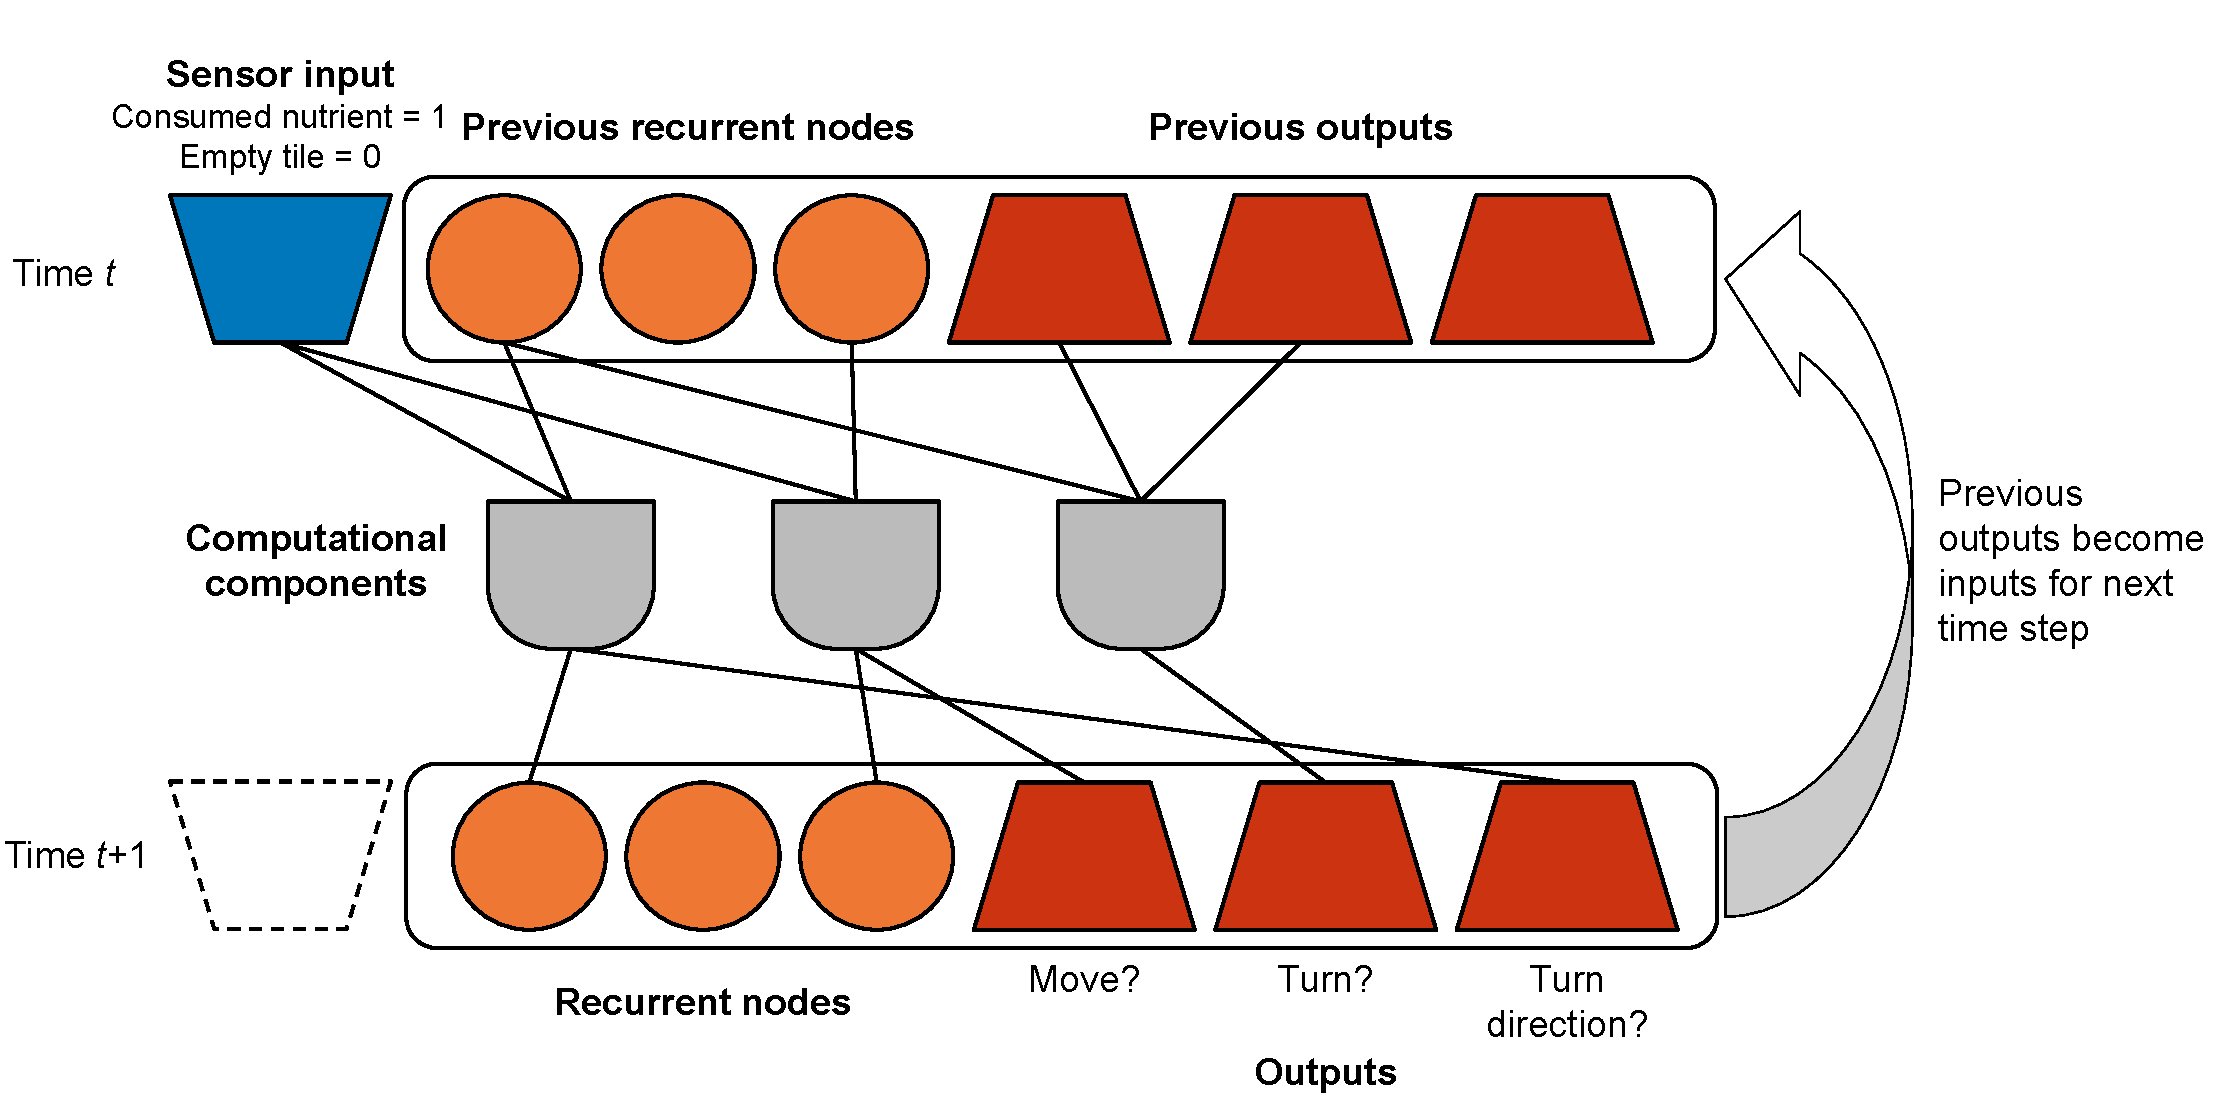
\includegraphics[width=0.95\textwidth]{07_potentiation_across_representations/media/markov_brain_conceptual_figure.pdf}
    \caption{Conceptual diagram of a Markov brain with inputs and outputs for the patch harvesting task, adapted from \citep{hintzeMarkovBrainsTechnical2017}.
    The single input, corresponding to the type of tile the organism is on, is shown as a blue trapezoid. 
    This example has three recurrent nodes (shown as orange circles) and three computational components (shown in gray). 
    The patch harvesting environment has three outputs, shown here as red trapezoids. 
    Note that the recurrent and output nodes (i.e., those in the rounded rectangle) will be passed as input in the next time step.
    The sensor input must come from the environment, as shown by the dashed trapezoid in the \textit{t+1} buffer.}
    \label{fig:varying_representations:markov_brain}
\end{figure}

% Go into more detail on how the brains work? Encoding?
Figure \ref{fig:varying_representations:markov_brain} shows an example Markov brain in the patch harvesting environment. 
At a given timestep \textit{t}, the organism will receive one input, some number of recurrent nodes, and three outputs (inputs and outputs described in the next subsection).
The genome of a particular brain encodes some number of computational components, including which inputs and outputs they are connected to. 
The inputs at timestep \textit{t} are passed into these computational components, and the outputs are written into an output buffer that includes recurrent nodes and output nodes (i.e., actuators). 
The environment will read the outputs and perform the appropriate actions, as described below. 
Finally, the recurrent and output nodes are passed back to the brain as part of the input buffer for time \textit{t+1}. 
This process constitutes one update, and each Markov brain will be executed for a given number of updates in order to perform its actions in the environment. 
A full description of Markov brains is available in \citep{hintzeMarkovBrainsTechnical2017}.

Computational components perform the transformation of inputs to outputs at each timestep. 
Here, I will only use deterministic logic gates for computational components, as they should be sufficient given that memory is already available via recurrent nodes. 
These logic gates take in some number of inputs and produce some number of outputs, with each deterministic logic gate containing its own truth table to map from inputs to outputs. 
For a given Markov brain, its computational components are all encoded in its genome. 
While we will avoid the details of the encoding (see \citep{hintzeMarkovBrainsTechnical2017} for details on computational components, logic gates, and the encoding scheme), it is important to note that Markov brains use a genetic encoding as compared to Avida's direct encoding. 
This allows for more flexibility in what effects mutations can have in a Markov brain. 
In our previous Avida work, a mutation always adds, removes, or swaps a single instruction. 
Mutations in Markov brains can have more minute difference, such as changing the type of computational component, modifying input/output connections, or changing the truth table of a logic gate. 
Combined with the fact that many sites in a Markov brain can be non-coding, these genomes have many possibilities for neutral and nearly-neutral mutations.
Additionally, the different effects that mutations can have create many a different suite of potential epistatic interactions than those found in Avida. 
Since we expect that epistatic interactions play a key role in the potentiation of a genome, these differences will likely influence how potentiation changes in Markov brains. 

\subsection{Changes to the patch harvesting environment and evolution system}

% We can't just throw Markov brains in the environment, we need to make a few changes
In Avida, the patch harvesting environment adds four new instructions: \texttt{Turn Left}, \texttt{Turn Right}, \texttt{Move Forward}, and \texttt{Sense}.
These instructions allow the organisms to pull information from the environment and take actions. 
Since Markov brains do not operate on the basis of instructions, we need to make some modifications to how the environment handles inputs and outputs. 

% How to modify IO
Instead of a \texttt{Sense} instruction that pulls the current tile's information into a register, to support Markov brains we will place the current tile's cue in the input buffer. 
Avida organisms work on 32-bit integers while Markov brains work on binary signals, so we will also need to convert the data itself. 
Because organisms consume food when they move on a tile, they can only encounter two types of tile cues: an empty tile or a tile that previous had food that has since been consumed. 
As such, we will place a one in the organism's input buffer if the tile previously contained food, or a zero if the tile has always been empty. 
Similarly, we need to determine what actions the organism will take based on the output buffer. 
To do this, we will give the organisms three bits of output. 
The first bit corresponds to movement; the organism will move forward if the movement bit is set. 
The last two bits will be used for turning. 
The first turning bit will determine if the organism will turn, while the second turning bit will determine which direction the organism will turn. 
Turning will be overridden by moving. 
Using two different bits to determine if the organism moves and if it turns allows for time steps with no environmental actions taken while still performing computation into the memory bits. 
With these modifications, the Markov brain organisms will have the pieces to sense their environment, do computation using normal Markov brain gates, and perform actions via their outputs. 

% Evolution system now needs to be synchronous 
The scoring of the environment and the classification of behaviors does not need to change from the Avida implementation. 
Organisms will still be rewarded for consuming food and punished for wandering into empty tiles. 
However, the evolution system itself will need to change to accommodate the change in representation. 
Avida operates on the concept of asynchronous generations -- organisms replicate themselves by executing certain instructions. 
This concept does not exist in Markov brains, so they must be externally replicated. 
As such, the Markov brains will evolve in a synchronous generation system. 
All organisms in the population will be evaluated independently to calculate their scores. 
Once the scores have been collected, we will select parents for the next generation by applying roulette (fitness proportional) selection, as it is the most similar to how Avida doles out updates. 
After replicating the parents and applying mutations, we will have our next generation and can restart the process.
We will conduct some preliminary experiments to ensure that Markov brains receive a comparable amount of time in the environment and comparable number of generations to the Avida organisms of Chapter \ref{chap:varying_environments}.


\section{Proposed work}

As in Chapter \ref{chap:varying_environments}, the main goal of this chapter is to replicate the potentiation analyses in Chapter \ref{chap:replaying_associative_learning} so we can then compare across systems. 
Here, this means we will be comparing potentiation along Markov brain lineages in the patch harvesting environment to Chapter 
\ref{chap:varying_environments} results on Avida lineages in the same environment.

Even though this chapter examines potentiation in Markov brains, a totally different substrate, our analyses of potentiation should be just as applicable. 
As such, I propose to conduct the same analyses as in Chapters \ref{chap:replaying_associative_learning} and \ref{chap:varying_environments}. 
Although this system uses synchronous generations, I can still track genotypic phylogenies and thus can conduct the two-phase replay experiments in the same way. 
As before, I will start by identifying the first genotype in the lineage that exhibits the target behavior and then seeding exploratory replay replicates 50, 100, 150, and 200 steps earlier in the lineage, launching additional replicates as needed until we reach the threshold of fewer than 10 percentage points of potentiation above the value found at the ancestor. 
I will then identify potentiation windows as done in previous chapters and run targeted replay replicates for each genotype in the windows. 

Once the replays have finished, the rest of the analysis is effectively identical to Chapter \ref{chap:varying_environments}. 
I will collect the measures of potentiation defined in Section \ref{sub:potentiation_measures}. 
Then I will statistically compare these measurements with the results of potentiation of Avida lineages on the patch harvesting tasks in Chapter \ref{chap:varying_environments}. 
Since each measurement is only comparing between two distributions (Avida versus Markov brains), we can simply conduct Mann-Whitney-Wilcoxon tests to look for statistical differences between the two \citep{10.2307/3001968}. 

This work will be the first direct comparison of how potentiation changes along successful lineages under different representations. 
I hypothesize that see similar trends in potentiation between the two representations. 
However, due to key differences, such as built-in memory in Markov brains or the differences in neutrality of the fitness landscape due to encodings, I expect the actual values of the measurements to differ between representations. 
% I do, however, expect the built-in memory to cause differences in some measurements, such as the number of potentiation windows. 
In Avida, evolving a strategy to successfully consume a single patch can be difficult to evolve (per preliminary work for Chapter \ref{chap:varying_environments}), and then evolving patch-switching behavior beyond that is an additional challenge. 
Thus I expect Avida to have two potentiation windows, on average, one for evolving the initial patch-harvesting behavior and a second for the patch-switching behavior.
My hypothesis is that the built-in memory of Markov brains eases the evolution of patch switching, resulting in one potentiation window in a typical Markov brain window, corresponding to the patch-harvesting behavior. 
In this case, I expect the Markov brain lineages to experience more potentiating gain in that single window, or more slow accumulation of potentiation. 
No matter what the results ultimately show, this work will be a solid step in exploring how potentiation changes; in combination with Chapters \ref{chap:replaying_associative_learning} and \ref{chap:varying_environments}, this work will complete the set of investigating potentiation when we vary the environment or the underlying organismal representation. 
These results will therefore be invaluable in future works in potentiation, whether they be theoretical, digital, or microbial.
\chapter{Concluding thoughts}
\label{chap:timeline}

\section{Outlook}

In this dissertation proposal I have outlined my plans to study how history interacts with adaptation and chance to produce cognitive behaviors. 
Specifically, I first demonstrated the power of analytic replay experiments \textit{in silico}, and I proposed to expand these studies to create the first large, cross-lineage dataset of how potentiation changes along successful lineages. 
Next, I proposed shifting to a simpler bitstring model to further develop our intuition and analysis techniques for potentiation. 
Taking a step back, I examined how the evolution of phenotypic plasticity influences future evolutionary dynamics, finding that plasticity stabilizes evolution. 
Finally, I proposed to study potentiation in two additional environments to test the generalizability of my earlier findings as the study system changes. 
%Specifically, the first two chapters demonstrate the power of analytic replay experiments \textit{in silico} by generating the first large cross-lineage dataset of how potentiation changes along successful lineages. 
%By examining this potentiation of associative learning, I can begin to identify general trends in how potentiation arises and any properties shared by mutations that influence it. 
%Further, these data will provide a point of comparison for future studies of potentiation, whether those be \textit{in silico} or \textit{in vivo}.
%Next I proposed a 

This proposal originally had one more chapter: an alternative proposal to study potentiation in different representations. 
Specifically, I would repeat the potentiation study in the patch harvesting environment using Markov brains, recurrent neural networks, and Cartesian genetic programming. 
By keeping the environment the same, this would demonstrate how potentiation dynamics change with the representation.  
While this chapter has been cut for brevity, it remains an option if a proposed chapter encounters unsalvageable issues or if my committee prefers it to another chapter. 

%Overall, this work asks important questions about the interplay of adaptation, chance, and history in the evolution of particular traits. 
The nature of this work is mostly exploratory; prior work has measured potentiation in specific systems, but not enough work has been conducted to begin drawing general conclusions about potentiation. 
This is the gap I aim to fill. 
While all the work I have proposed is digital, by studying different environments and representations, I will create intuition about potentiation that is likely to extend beyond digital systems.
Doing this work \textit{in silico} is required, however, as the work that I have proposed is currently intractable to conduct \textit{in vivo}.
Regardless, here I expand on the previous work on microbial potentiation to help us understand how adaptation, chance, and history interact to create the diverse complexity we see in the world. 

There are countless ways the work in this proposal could be extended. 
Since this area is so new and so difficult to study in wetlab systems, quantifying potentiation after varying \textit{any} aspect of the system can provide new insights into how potentiation arises and the forms that it takes. 
For example, while the cyclic logic 6 environment of Chapters \ref{chap:consequences_of_plasticity} and \ref{chap:varying_environments} changes over time, a more systematic study of the effects of temporal changes on potentiation would be relevant for many natural systems, where both biotic and abiotic factors are constantly changing. 
I am particularly interested the fundamentals of potentiation, and as such I am curious how potentiation changes in other simple models like the NK landscapes of Chapter \ref{chap:simplified_model}.
Specifically, I am interested in the effect of switching from bitstrings to multi-allele representations. 
When targeting only single trait in a bitstring model, every single-bit mutation must bring you either closer or farther away from that trait. 
By switching to a multi-allele model, we could analyze mutations that are neutral with respect to the genetic distance to the target. 
Finally, the analyses here focus on target traits that are effectively optimal, but this is not required. 
How do potentiation dynamics change as we switch to targeting suboptimal traits, and how does the potentiation of one trait affect the potentiation of other traits?
These ideas only begin to scratch the surface of possibilities in studying potentiation dynamics, and it will be exciting to see how this area of evolutionary biology develops over the coming decades. 

% [I keep wanting to explain why these chapters are repetitive. That's the point! I'll be running the same experiment 3 or 4 times with slightly different setups to give us initial data to compare how potentiation changes. Did this get across? I don't think so]

% In writing this proposal, I have had a few nagging concerns in the back of my mind and want to discuss them briefly here. 

% First and foremost, the four proposed chapters feel repetitive and lacking in literature depth. 
% This issue has bothered me throughout writing this document. 
% At the end of the day, I have come to realize that my main goal in those chapters was to show how 


% In writing this dissertation proposal, I cannot help but think that it feels very different than those that I have read before from friends and colleagues. 
% Last year at my first committee meeting, I mentioned that I was working on what is now \ref{chap:alife_submission}, but that most of my time had been spent implementing the basics of Avida in MABE2. 
% This has greatly shaped the second half of my PhD. 
% While re-implementing Avida, I conducted research, but most of it does not fit this theme and is thus is not included in this dissertation proposal. 
% As such, it feels like I am proposing an insane amount of work, though the proposal chapters themselves feel repetitive. 
% I would like to speak on that briefly here. 

% In writing this dissertation proposal, I the proposed chapters were repetitive and lacking in literature depth. 
% I am a slow writer, which means that I have sat with these thoughts for quite a while, and I have some thoughts. 
% The chapters are repetitive due to the nature of what I have proposed in this document. 
% Proposals should include two things: the work you will be doing and why it matters. 
% In both cases, these do not change much between the potentiation chapters. 
% The only variation in methods is how I will be varying the environment or representation, while the positioning in the literature is constant across chapters. 

% Beyond the literature and methods, all proposed chapters have effectively the same end goal: to generate initial data so we can begin to hypothesize about how potentiation occurs in different system, and if any general rules or patterns exist. 

\section{Proposed timeline}

I have outlined a substantial amount of work of be done in this proposal. %you probably realized while reading through the chapters, I have proposed a substantial amount of work. 
The three proposed chapters require huge amounts of time just to generate the data, which is compounded by analysis and writing. 
I have attempted to trim the fat where possible, reducing the amount of computation needed for each chapter. 
Even still, my current plan is to defend late next spring.
To have any hope of meeting that deadline, I need a plan. 
Therefore, I present my timeline for when I will perform the various tasks for each chapter Figure \ref{fig:timeline}. %, with some extra about the time required for each task. 

% Go into more detail on how the brains work? Encoding?
\begin{figure}[h!]
    \centering
    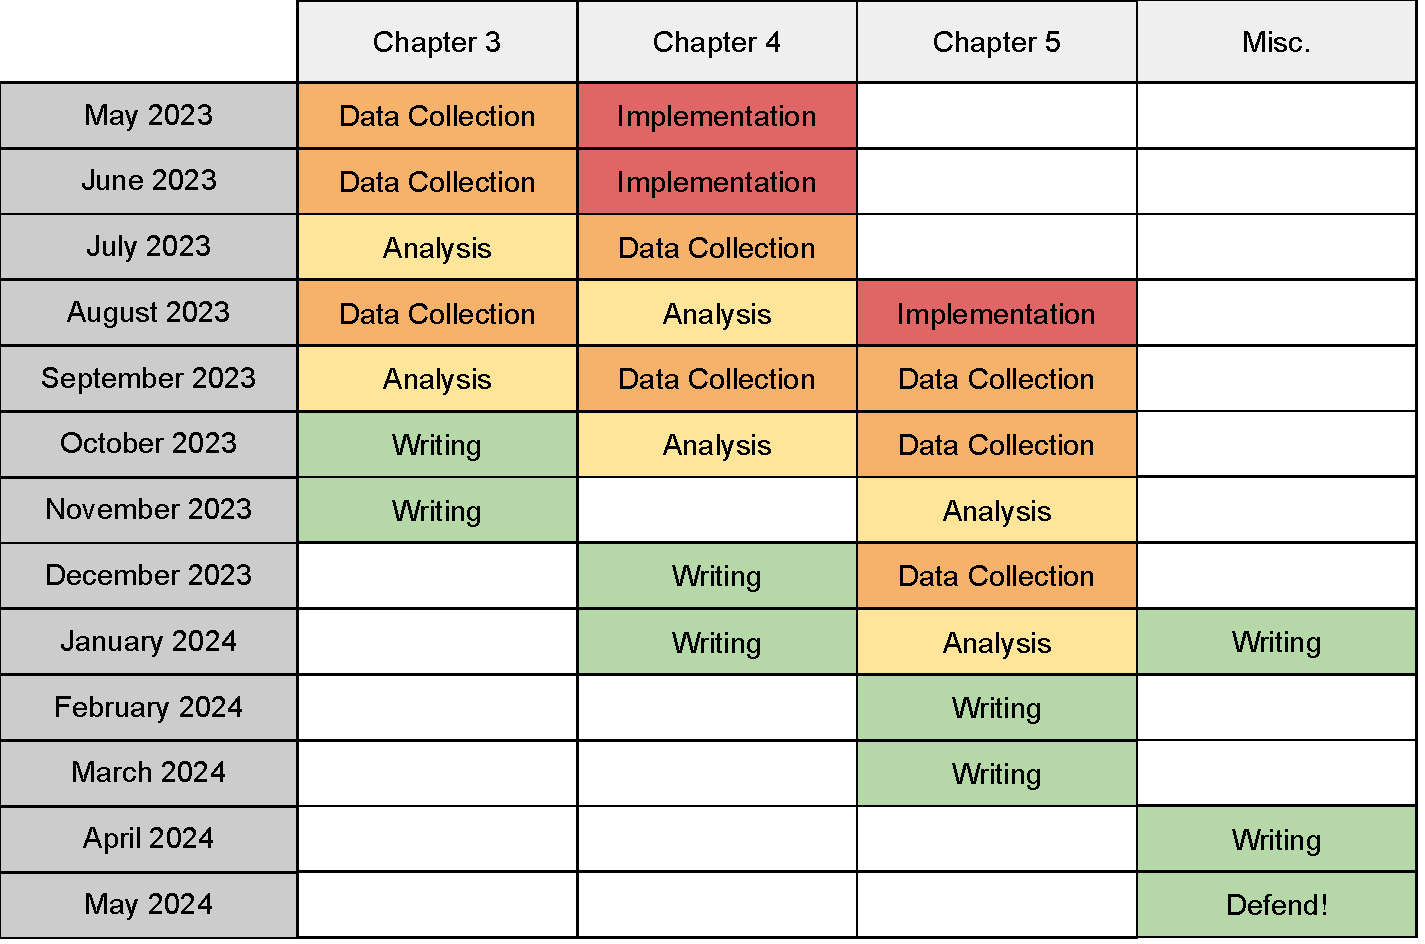
\includegraphics[width=0.95\textwidth]{08_timeline/media/timeline.pdf}
    \caption{My proposed timeline for completing the proposed chapters and my dissertation as a whole. 
    The miscellaneous column includes writing the introduction and conclusion of the dissertation.
    Remainder of explanation in text.}
    \label{fig:timeline}
\end{figure}


As stated above, all three proposed chapters, but especially Chapters \ref{chap:replaying_associative_learning} and \ref{chap:varying_environments}, are very computationally expensive. Thus I have included two initial months of data collection for both, with an extra month allotted for any additional data collection that was identified as needed during analysis. 
The other chapter, Chapter \ref{chap:simplified_model}, will deal with an enormous amount of data, but the bitstring model makes that data much faster to collect. 
As such, it receives only one month of initial data collection and one month for collecting any additional data. 
%It should be noted that once the pipeline for collecting data is in place, collecting data is mostly a hands off process, allowing me to perform other tasks at the same time.
%I have created infrastructure to allow thousands of jobs to queue and run on the HPCC with no human oversight needed. 

Chapter \ref{chap:replaying_associative_learning} is not allotted any dedicated implementation time, as all the pieces are in place thanks to Chapter \ref{chap:alife_submission}.
This chapter is ready to begin data collection once the comprehensive examination has concluded.
Chapter \ref{chap:simplified_model} is allotted a very conservative two months of implementation, as all the pieces (NK landscapes, enumeration and replay pipelines) exist and will only require tweaks and testing. 
Finally, all the environments and Avida changes are already implemented in MABE2, and thus Chapter \ref{chap:varying_environments} is given a single month of dedicated implementation time to connect the pieces together. 

Each project is given two months for analysis, one after the initial data collection and one more after any additional data collection is completed. 
%Note that once the analyses have been created, I will be running many of these analyses as soon as the data is finished and pulled from the HPCC. 
%As such, I will often be performing other tasks, such as writing or implementing, during the months marked as analysis. 

Finally, all of these projects will need to be written up. %, and writing is the hardest for me to judge the time required. 
As things stand, I have allotted two months of writing time for each proposed chapter. 
I have also allotted two months to writing the other pieces of the dissertation (e.g., introduction, conclusion, and any needed appendices). 

Fortunately, data collection is mostly hands-off once it has been started, and most analyses will be reused for the various projects, saving substantial time in the long run. 
%It is not shown, but I will also be drafting the early parts of each chapter (e.g., the introduction and methods) as I collect data and analyze the data. 
Having different projects going simultaneously is my preferred way to work, as I often switch between them when I hit a rut, allowing me to come back later with a fresh mind. 
As such, I have attempted to structure this timeline such that I always have one active task (coding or writing) occurring concurrently with data collection and analysis. 
While I could not easily show it in the figure, I will begin writing the introduction and methods to each chapter during the early data collection and analysis phases. 

While it will be a ton of work, I look forward to it. 
%I have tried to structure this timeline in a way that I am often collecting data for one project while doing writing, coding, or analyzing one or two other chapters, as data collection does not require much active effort in these systems. 


% Mention that I will be TAing in the fall but not the spring?


% \part{Designing Computational Infrastructure to Enable Scalable Digital Multicellularity Experiments} \label{part:infrastructure}
% \include{tex/body/conduit}
% \include{tex/body/distributed-phylogeny}
% \part{Evolving Complexity, Novelty, and Adaptation in Digital Multicells} \label{part:experiments}
% \include{tex/body/case-studies}
% \include{tex/body/measuring-cna}
% \include{tex/body/conclusion}

\clearpage

\begin{singlespace}
\addcontentsline{toc}{chapter}{BIBLIOGRAPHY}
\renewcommand{\bibsection}{\centerline{\textbf{BIBLIOGRAPHY}}}
\bibliographystyle{apalike}% your bst file here
\bibliography{ferguson_comps} %your bib file here
\end{singlespace}

%%%  Appendices, if necessary: I don't have any @jgh9094

\end{doublespace}
\end{document}
